% Customizable fields and text areas start with % >> below.
% Lines starting with the comment character (%) are normally removed before release outside the collaboration, but not those comments ending lines

% svn info. These are modified by svn at checkout time.
% The last version of these macros found before the maketitle will be the one on the front page,
%so only the main file is tracked.
% Do not edit by hand!
\RCS$Revision: 343919 $
\RCS$HeadURL: svn+ssh://svn.cern.ch/reps/tdr2/notes/AN-14-135/trunk/AN-14-135.tex $
\RCS$Id: AN-14-135.tex 343919 2016-05-23 16:05:58Z lfinco $
%%%%%%%%%%%%% local definitions %%%%%%%%%%%%%%%%%%%%%
%\usepackage{rotating}
%\usepackage{float}
%\usepackage[utf8]{inputenc}
% This allows for switching between one column and two column (cms@external) layouts
% The widths should  be modified for your particular figures. You'll need additional copies if you have more than one standard figure size.
\newlength\cmsFigWidth
\ifthenelse{\boolean{cms@external}}{\setlength\cmsFigWidth{0.85\columnwidth}}{\setlength\cmsFigWidth{0.4\textwidth}}
\ifthenelse{\boolean{cms@external}}{\providecommand{\cmsLeft}{top}}{\providecommand{\cmsLeft}{left}}
\ifthenelse{\boolean{cms@external}}{\providecommand{\cmsRight}{bottom}}{\providecommand{\cmsRight}{right}}
%%%%%%%%%%%%%%%  Title page %%%%%%%%%%%%%%%%%%%%%%%%
\cmsNoteHeader{AN-14-135} % This is over-written in the CMS environment: useful as preprint no. for export versions
% >> Title: please make sure that the non-TeX equivalent is in PDFTitle below
\title{Measurement of the differential cross section for $pp\rightarrow ZZ \rightarrow 4 \ell$ produced in association with jets in pp collisions at $\sqrt{s}=13$~TeV}

% >> Authors
%Author is always "The CMS Collaboration" for PAS and papers, so author, etc, below will be ignored in those cases
%For multiple affiliations, create an address entry for the combination
%To mark authors as primary, use the \author* form

\address[unito]{Universi\`a degli Studi di Torino and INFN.}
\address[infnto]{INFN Torino.}
\address[hig]{The Higgs to four leptons team.}
\author[unito]{N. Amapane}
\author[unito]{R. Bellan} 
\author[unito]{R. Covarelli} 
\author[unito]{L. Finco}
\author[unito]{R. Gomez Ambrosio}
\author[infnto]{C. Mariotti}  
\author[unito]{G. Pinna}
\author[hig]{many other people}

% >> Date
% The date is in yyyy/mm/dd format. Today has been
% redefined to match, but if the date needs to be fixed, please write it in this fashion.
% For papers and PAS, \today is taken as the date the head file (this one) was last modified according to svn: see the RCS Id string above.
% For the final version it is best to "touch" the head file to make sure it has the latest date.
\date{\today}

% >> Abstract
% Abstract processing:
% 1. **DO NOT use \include or \input** to include the abstract: our abstract extractor will not search through other files than this one.
% 2. **DO NOT use %**                  to comment out sections of the abstract: the extractor will still grab those lines (and they won't be comments any longer!).
% 3. For PASs: **DO NOT use tex macros**         in the abstract: CDS MathJax processor used on the abstract doesn't understand them _and_ will only look within $$. The abstracts for papers are hand formatted so macros are okay.
\abstract{This note reports the measurement of the differential cross sections of two Z bosons produced in association with jets in pp collisions at a center-of-mass energy of $\sqrt{s}=13~\mathrm{TeV}$. This analysis is based on a data sample collected with the CMS experiment at the LHC, corresponding to an integrated luminosity of $12.9~\mathrm{fb}^{-1}$. Measurements are performed in the leptonic decay modes $\mathrm{ZZ}\to\ell\ell\ell'\ell'$, where $\ell,\ell' = e, \mu$. 
}

% >> PDF Metadata
% Do not comment out the following hypersetup lines (metadata). They will disappear in NODRAFT mode and are needed by CDS.
% Also: make sure that the values of the metadata items are sensible and are in plain text:
% (1) no TeX! -- for \sqrt{s} use sqrt(s) -- this will show with extra quote marks in the draft version but is okay).
% (2) no %.
% (3) No curly braces {}.
\hypersetup{%
pdfauthor={R. Bellan, L. Finco},%
pdftitle={Measurement of the differential cross section for ZZ rightarrow 4 ell produced in association with jets in pp collisions at sqrt s = 13 TeV},%
pdfsubject={CMS},%
pdfkeywords={CMS, physics, software, computing}}

\maketitle %maketitle comes after all the front information has been supplied
% >> Text
%%%%%%%%%%%%%%%%%%%%%%%%%%%%%%%%  Begin text %%%%%%%%%%%%%%%%%%%%%%%%%%%%%
%% **DO NOT REMOVE THE BIBLIOGRAPHY** which is located before the appendix.
%% You can take the text between here and the bibiliography as an example which you should replace with the actual text of your document.
%% If you include other TeX files, be sure to use "\input{filename}" rather than "\input filename".
%% The latter works for you, but our parser looks for the braces and will break when uploading the document.
%%%%%%%%%%%%%%%

\tableofcontents

%%%%%%%%%%%%%%%%%%%%%%%%%%%%%%%%  Begin text %%%%%%%%%%%%%%%%%%%%%%%%%%%%%


%% --------------------------------------------------------- %%
\section{Introduction}
\label{sec:introduction}
In this note we present the measurement of the differential cross section of two Z bosons produced in association with jets in pp collisions at $\sqrt{s}= 13~\mathrm{TeV}$, extending the analysis performed at $\sqrt{s}= 8~\mathrm{TeV}$ in~\cite{CMS-PAS-SMP-15-012}. The dependence of the cross section on jet multiplicity tests the current understanding of the QCD corrections to ZZ production. Moreover, the study of the invariant mass of the two $p_T$-leading jets ($m_{jj}$) establishes the basis for future multi-boson final state searches and for the investigation of phenomena involving interactions with four bosons in a single vertex. Finally, the measurement of the separation in pseudorapidity between the two $p_T$-leading jets ($\Delta\eta_{jj}$) is instrumental for the vector boson scattering analysis in this channel, the key process to probe the nature of the electroweak symmetry breaking mechanism, which becomes potentially accessible at 13 TeV.\\
 The measurement is performed considering the \Z bosons decaying leptonically to either electrons or muons. The analysis is based on a data set that corresponds to an integrated luminosity of $12.9~\mathrm{fb}^{-1}$, collected by the CMS experiment at $\sqrt{s} =$~ 13 TeV.\\

The implant of the analysis is largely the same as~\cite{CMS-PAS-SMP-15-012} and, for what concerns the reconstruction of the two Z bosons, it is explicitly
based on the algorithms and the techniques used for the $H\rightarrow ZZ \rightarrow 4\ell$ analysis~\cite{HiggsLegacyPaper} (as it was done for~\cite{CMS-PAS-SMP-15-012}), with the obvious change in the mass window ($60 < m_{Z_{1,2}} < 120~\mathrm{GeV}$). %used for the lowest quality Z.


This note is organized as follow: section~\ref{sec:samples} summarizes the Monte Carlo and the dataset used for this analysis, section~\ref{sec:selection} describes the event selection, 
while section~\ref{sec:background} deals with the background estimation and the related uncertainties. Section~\ref{sec:systunc} lists the several sources of systematic uncertainty and, finally, in section~\ref{sec:results} we present the result of this analysis,
including the unfolding of the detector resolution for the differential cross-section that we measured.
 

%% --------------------------------------------------------- %%


%% --------------------------------------------------------- %%
\section{The CMS Detector and MC Samples}
\label{sec:samples}
A more detailed description of the CMS detector, together with a definition of the coordinate system used and the relevant kinematic variables, can be found in~\cite{CMS}; the key components for this analysis are summarized here. The CMS experiment is characterized by a superconducting solenoid located in the central region of
the detector, providing an axial magnetic field of 3.8 T parallel to the beam direction. A silicon pixel and strip tracker, a crystal electromagnetic calorimeter (ECAL), and a brass and scintillator hadron calorimeter are located within the solenoid and cover the absolute pseudorapidity range $|\eta| < 3.0$, where pseudorapidity is defined as $\eta = - \mathrm{ln}[\mathrm{tan}(\theta/2)]$. The Forward Hadronic calorimeters (HF) are placed outside the magnet yoke, 11 m far from the interaction point, extending the pseudorapidity coverage up to $|\eta|= 5$. \\

Several Monte Carlo (MC) event generators are used to simulate the signal and background contributions. The MC samples are employed to optimize the event selection, evaluate the signal efficiency and acceptance, estimate the irreducible background yields and extract the unfolding response matrices used to statistically remove experimental effects from data distributions.\\
FIXME
%We use a simulation for signal processes that is largely the same as that adopted in~\cite{CMS-PAS-SMP-15-012}. Differently from the previous published analysis (FIXME MC SAMPLES), 
%the $\cPq\cPaq \to \Z\Z$ and $\cPg\cPg \to \Z\Z\cPq\cPq$ (tree-level only) processes are produced at leading-order (LO) for 0, 1 and 2 jets with \texttt{MadGraph 5.1}~\cite{MadGraph5.1}, and are compared with the inclusive ZZ production generated using \texttt{Powheg 2.0} at next-to-leading order (NLO)~\cite{PowhegMethod, PowhegBox, Melia:2011tj, Nason:2013ydw}. Since the latter does not contain events with 2 jets from the hard process, the \texttt{MadGraph} sample is expected to describe better the variables related to jets. The signal cross section is scaled to match the theoretical ZZ cross section calculated with \texttt{MCFM}~\cite{MCFM} at NLO. The \texttt{MadGraph5\_aMCatNLO} generator, which simulates signal processes at NLO for 0 and 1 jet, is also used for comparison purposes at generator level~\cite{MGatNLO}.  \\
%Furthermore,  the $\cPg\cPg  \to \Z\Z$ (box diagrams) processes are generated at LO with \texttt{MCFM 6.7} instead of \texttt{GG2ZZ}~\cite{gg2zz}. Finally, vector boson scattering processes with two Z bosons produced in association with 2 forward and backward jets, which were not considered in the previous analysis, are simulated using \texttt{Phantom}~\cite{Phantom}.\\
%Other diboson and triboson processes (WZ, Zg, ZZZ, WZZ, WWZ) and the Z + jets samples are generated at LO with \texttt{MadGraph}, like events from \ttbar production. The \texttt{PYTHIA 6.4}~\cite{Sjostrand:2006za} package is used for parton showering, hadronization, and the underlying event simulation for all MC samples but \texttt{MadGraph5\_aMCatNLO}, in which  \texttt{PYTHIA 8.0}~\cite{Sjostrand:2007gs} is employed. The default set of parton distribution functions (PDF) used for LO generators is \texttt{CTEQ6L}~\cite{CTEQ6L}, whereas \texttt{CT10}~\cite{CT10} is used for NLO generators.

%%\begin{table*}[htbH]\footnotesize
%\begin{sidewaystable}\footnotesize
%\begin{center}\scriptsize
%\topcaption{List of signal and background samples used in the analysis.}
%\label{tab:listofsamples}
%\begin{tabular}{lll}
%\hline  Process & Cross Sections [pb] & Sample\\
%\hline  \multicolumn{3}{l}{Signal Samples}\\
%$ZZ\to 4\ell$ (\texttt{MadGraph}) & 0.071 (no $\tau$) & \texttt{ZZJetsTo4L\_TuneZ2star\_8TeV-madgraph-tauola/Summer12\_DR53X-PU\_S10\_START53\_V7A-v1/AODSIM/PAT\_CMG\_V5\_15\_0/} \\ 
%$q\bar{q}\to ZZ\to 4\mu$ (\texttt{Powheg}) & 0.07691 & \texttt{ZZTo4mu\_8TeV-powheg-pythia6/Summer12\_DR53X-PU\_S10\_START53\_V7A-v1}\\
%$q\bar{q}\to ZZ\to 4e$  (\texttt{Powheg}) & 0.07691 & \texttt{ZZTo4e\_8TeV-powheg-pythia6/Summer12\_DR53X-PU\_S10\_START53\_V7A-v1 }\\ 
%$q\bar{q} \to ZZ\to 2e2\mu$  (\texttt{Powheg})& 0.1767 & \texttt{ZZTo2e2mu\_8TeV-powheg-pythia6/Summer12\_DR53X-PU\_S10\_START53\_V7A-v1}\\ 
%$gg\to ZZ\to 4\mu$  (\texttt{MCFM})&0.000592340 &\texttt{GluGluTo4mu\_SMHContinInterf\_M-125p6\_8TeV-MCFM67-pythia6/Summer12\_DR53X-PU\_S10\_START53\_V19-v1 }\\
%$gg\to ZZ\to 4e$  (\texttt{MCFM}) &0.000592000 &\texttt{GluGluTo4e\_SMHContinInterf\_M-125p6\_8TeV-MCFM67-pythia6/Summer12\_DR53X-PU\_S10\_START53\_V19-v1 }\\ 
%$gg\to ZZ\to 2e2\mu$  (\texttt{MCFM})& 0.00118409 & \texttt{GluGluTo2e2mu\_SMHContinInterf\_M-125p6\_8TeV-MCFM67-pythia6/Summer12\_DR53X-PU\_S10\_START53\_V19-v1}\\
%$ZZ\to 4\mu +2jets$  (\texttt{Phantom})&2.49E-04 & \texttt{ZZTo4muJJ\_SMHContinInterf\_M-125p6\_8TeV-phantom-pythia6/Summer12\_DR53X-PU\_S10\_START53\_V19-v1}\\ 
%$ZZ\to 4e +2jets$  (\texttt{Phantom})& 2.48E-04&\texttt{ZZTo4eJJ\_SMHContinInterf\_M-125p6\_8TeV-phantom-pythia6/Summer12\_DR53X-PU\_S10\_START53\_V19-v1}\\
%$ZZ\to 2e2\mu +2jets$  (\texttt{Phantom})&5.43E-04 &\texttt{ZZTo2e2muJJ\_SMHContinInterf\_M-125p6\_8TeV-phantom-pythia6/Summer12\_DR53X-PU\_S10\_START53\_V19-v1 }\\ 
%$WZZ + jets$ (\texttt{MadGraph}) & 0.01968& \texttt{WZZNoGstarJets\_8TeV-madgraph/Summer12\_DR53X-PU\_S10\_START53\_V7A-v1}\\
%$ZZZ + jets$ (\texttt{MadGraph}) &0.005527 &\texttt{ZZZNoGstarJets\_8TeV-madgraph/Summer12\_DR53X-PU\_S10\_START53\_V7A-v1 }\\
%$t\bar{t}+H$ (\texttt{Pythia}) & 0.0001081681 & \texttt{TTbarH\_HToZZTo4L\_M-126\_8TeV-pythia6/Summer12\_DR53X-PU\_S10\_START53\_V7C-v1}\\
%\hline  \multicolumn{3}{l}{Irreducible Background Samples}\\
%\hline$t\bar{t}+Z+Jets$ (\texttt{MadGraph})&0.2057 &\texttt{TTZJets\_8TeV-madgraph\_v2/Summer12\_DR53X-PU\_S10\_START53\_V7A-v1 }\\ 
%$t\bar{t}+WW+Jets$ (\texttt{MadGraph})&0.00208989 & \texttt{TTWWJets\_8TeV-madgraph/Summer12\_DR53X-PU\_S10\_START53\_V7A-v1}\\ 
%$WWZ + jets$ (\texttt{MadGraph}) &0.05795 & \texttt{WWZNoGstarJets\_8TeV-madgraph/Summer12\_DR53X-PU\_S10\_START53\_V7A-v1}\\
%\hline  \multicolumn{3}{l}{Reducible Background Samples}\\
%\hline $Z$ (\texttt{MadGraph})& 3503.71& \texttt{DYJetsToLL\_M-50\_TuneZ2Star\_8TeV-madgraph-tarball/Summer12\_DR53X-PU\_S10\_START53\_V7A-v1 }\\
%$WZ$ (\texttt{MadGraph})&1.057 & \texttt{WZJetsTo3LNu\_TuneZ2\_8TeV-madgraph-tauola/Summer12\_DR53X-PU\_S10\_START53\_V7A-v1}\\
%$WWW$ (\texttt{MadGraph})&0.08058 &\texttt{WWWJets\_8TeV-madgraph/Summer12\_DR53X-PU\_S10\_START53\_V7A-v1}\\
%$t\bar{t}+\gamma+Jets$ (\texttt{MadGraph})&1.93236 & \texttt{TTGJets\_8TeV-madgraph/Summer12\_DR53X-PU\_S10\_START53\_V7A-v1}\\
%$t\bar{t}\to 2\ell 2\nu 2B$ (\texttt{Powheg})&23.64 &\texttt{TTTo2L2Nu2B\_8TeV-powheg-pythia6/Summer12\_DR53X-PU\_S10\_START53\_V7A-v1 }\\
%$t\bar{t}+W+Jets$ (\texttt{MadGraph})&0.232 &\texttt{TTWJets\_8TeV-madgraph/Summer12\_DR53X-PU\_S10\_START53\_V7A-v1 }\\
%\hline
%\end{tabular}
%\end{center}
%\end{sidewaystable}
%%\end{table*}


%The data sets processed in this analysis are summarized in table~\ref{tab:datasamples}, along with the trigger selection operated on them (based on the same selection presented in~\cite{HiggsLegacyPaper, ZZXSPaper}).

%\begin{table*}
%\begin{center}
%\topcaption{List of data samples used in the analysis: 22Jan2013ReReco reprocessing of DoubleMu, DoubleEle, MuEG; total integrated luminosity
%of $19.7~\mathrm{fb}^{-1}$.}
%\label{tab:datasamples}
%\begin{tabular}{l}
%\hline  \textbf{Data Samples} \\
%\hline  DoubleMu/Run2012A-22Jan2013-v1\\
%DoubleMuParked/Run2012B-22Jan2013-v1\\
%DoubleMuParked/Run2012C-22Jan2013-v1\\
%DoubleMuParked/Run2012D-22Jan2013-v1\\
%DoubleElectron/Run2012A-22Jan2013-v1\\
%DoubleElectron/Run2012B-22Jan2013-v1\\
%DoubleElectron/Run2012C-22Jan2013-v1\\
%DoubleElectron/Run2012D-22Jan2013-v1\\
%MuEG/Run2012A-22Jan2013-v1\\
%MuEG/Run2012B-22Jan2013-v1\\
%MuEG/Run2012C-22Jan2013-v1\\
%MuEG/Run2012D-22Jan2013-v1\\
%\hline
%\end{tabular}
%\end{center}
%\end{table*}


%% --------------------------------------------------------- %%


%% --------------------------------------------------------- %%
\section{Event Recontruction and Selection}
\label{sec:selection}

%\fixme{This section needs to be rewritten to point to the relevant AN instead of copying and pasting them}

A complete reconstruction of the individual particles emerging from each collision event is obtained
via a particle-flow (PF) technique~\cite{CMS-PAS-PFT-09-001}, which uses the information from all CMS subdetectors. 
%to identify and reconstruct individual particles in the collision event. 
The identification of the particles produced in the event is the very same as the one described in~\cite{ZZXSPaper}, 
including the final state radiation treatment.
Also the logic to build up the ZZ candidate is the same as the Higgs boson analysis~\cite{HiggsLegacyPaper}.

The CMS standard selection of runs and luminosity sections is applied, which requires high quality data with a 
good functioning of the different sub-detectors. Events are selected online from the presence of a pair of electrons
or muons, or a triplet of electrons. Triggers requiring an electron and a muon are also used. The
minimal transverse momenta ($p_T$) of the first and second lepton are 17 and 8 GeV, respectively,
for the double lepton triggers, while they are 15, 8 and 5 GeV for the triple electron trigger.
More details can be found in~\cite{MuonTrigger}. The trigger efficiency for $ZZ$ events within the acceptance of this
analysis is greater than 98\%. % (to check, \fixme{}).\\

Events with identified and isolated primary electrons or muons are first selected by the offline
selection. We require a $Z$ candidate formed with a pair of leptons of the same flavor and
opposite charge. The FSR photons are kept if $|m_{\ell\ell\gamma} - m_Z | < |m_{\ell\ell} - m_Z | $ and $m_{\ell\ell\gamma} < 100$ GeV and
in the following the presence of the photons in the $\ell\ell$ kinematics is implicit.\\ 
The lepton pair with the invariant mass closest to the nominal $Z$ mass is denoted $Z_1$. A second $\ell^+\ell^-$ pair is required and denoted $Z_2$. If more than one $Z_2$ candidate satisfies all criteria, the pair of leptons with the highest scalar sum of $p_T$ is chosen. Both $Z$ candidates have to satisfy $60 < m_Z < 120$ GeV.
Among the four selected leptons forming the $Z_1$ and the $Z_2$ candidates at least one should have $p_T \ge 20$ GeV and another
one have $p_T \ge 10$ GeV  and any opposite-charge pair of leptons chosen among the four selected
leptons satisfy $m_{\ell\ell} \ge 4$ GeV. 
%Finally the phase space is reduced to the signal region by requiring $m_{4\ell} \ge 100$ GeV.

%\fixme{say here where the jets come from}
Jets are reconstructed using the anti-$k_{T}$ clustering 
algorithm~\cite{antiKT}, with a size parameter of $R = 0.5$, by summing the four-momenta of individual
PF particles according to the \texttt{FASTJET} package of reference~\cite{FASTJET}. Once reconstructed, jets overlapping
 (within $\Delta R = 0.5$) with any of the two leptons coming form the decay of the Z boson are removed from the jet collection. Jets satisfy the selection criteria recommended by Jet-MET group~\cite{JetID}. Jet energy corrections are applied as a function of the jet $p_T$ and $\eta$~\cite{JECandJER}. Moreover, they are required to have $p_T > 30$ GeV, 
 to reduce the pileup contamination as well as large uncertainty on the energy measurement, and $|\eta| < $ 4.7,
to ensure a good quality of the tracking information.
Since the jet energy resolution in data is worse than in simulation, the $p_T$ values of simulated
jets need to be smeared to describe data. Following the prescription of the CMS Jet-MET group~\cite{JETRES},
the corrected $p_T$ of the reconstructed jets are randomly smeared using a Gaussian distribution with a width 
of $\sqrt{c^2 -1}\cdot \sigma_{MC}$, 
where $c$ is the scaling factor (see Table~\ref{tab:c_JER}). This method only allows one to
worsen the resolution ($c > 1$). To determine the jet resolution in simulation, $\sigma_{MC}$, recommended tools have been used~\cite{JETRES}. 
\begin{table*}[htbH]
\begin{center}
\topcaption{Scaling factors applied on MC jets to described the data resolution\label{tab:c_JER}}
\begin{tabular}{cccccccc}
\hline $|\eta|$-region & $0.0-0.5$ & $0.5-1.1$ & $1.1-1.7$ & $1.7-2.3$ & $2.3-2.8$ & $2.8-3.2$ & $3.2-5.0$\\
\hline $c$ & 1.079 & 1.099 & 1.121 & 1.208 & 1.254 & 1.395 & 1.056\\
\hline
\end{tabular}
\end{center}
\end{table*}

Ancillary quantities, like data/MC efficiency scale factor and jet-to-lepton fake rate, are the same as the one measured in~\cite{ZZXSPaper}.

%% --------------------------------------------------------- %%


%% --------------------------------------------------------- %%
\section{Background Estimation}
\label{sec:background}
The lepton identification and isolation requirements significantly suppress
the background contribution, and the remnant portion of it is very small compared to the signal.
We can identify two main background components: an irreducible background from genuine four high-$p_T$ isolated leptons processes, such as $t\bar{t}Z$, $WWZ$ and $t\bar{t}WW$,  and a reducible background from processes with less than four leptons, but with jets that are misidentified as leptons. 

The irreducible background is very small and it is estimated using MC samples (see Fig.~\ref{fig:irr_bkg}).
\begin{figure}[hbtp]
  \begin{center}
   % 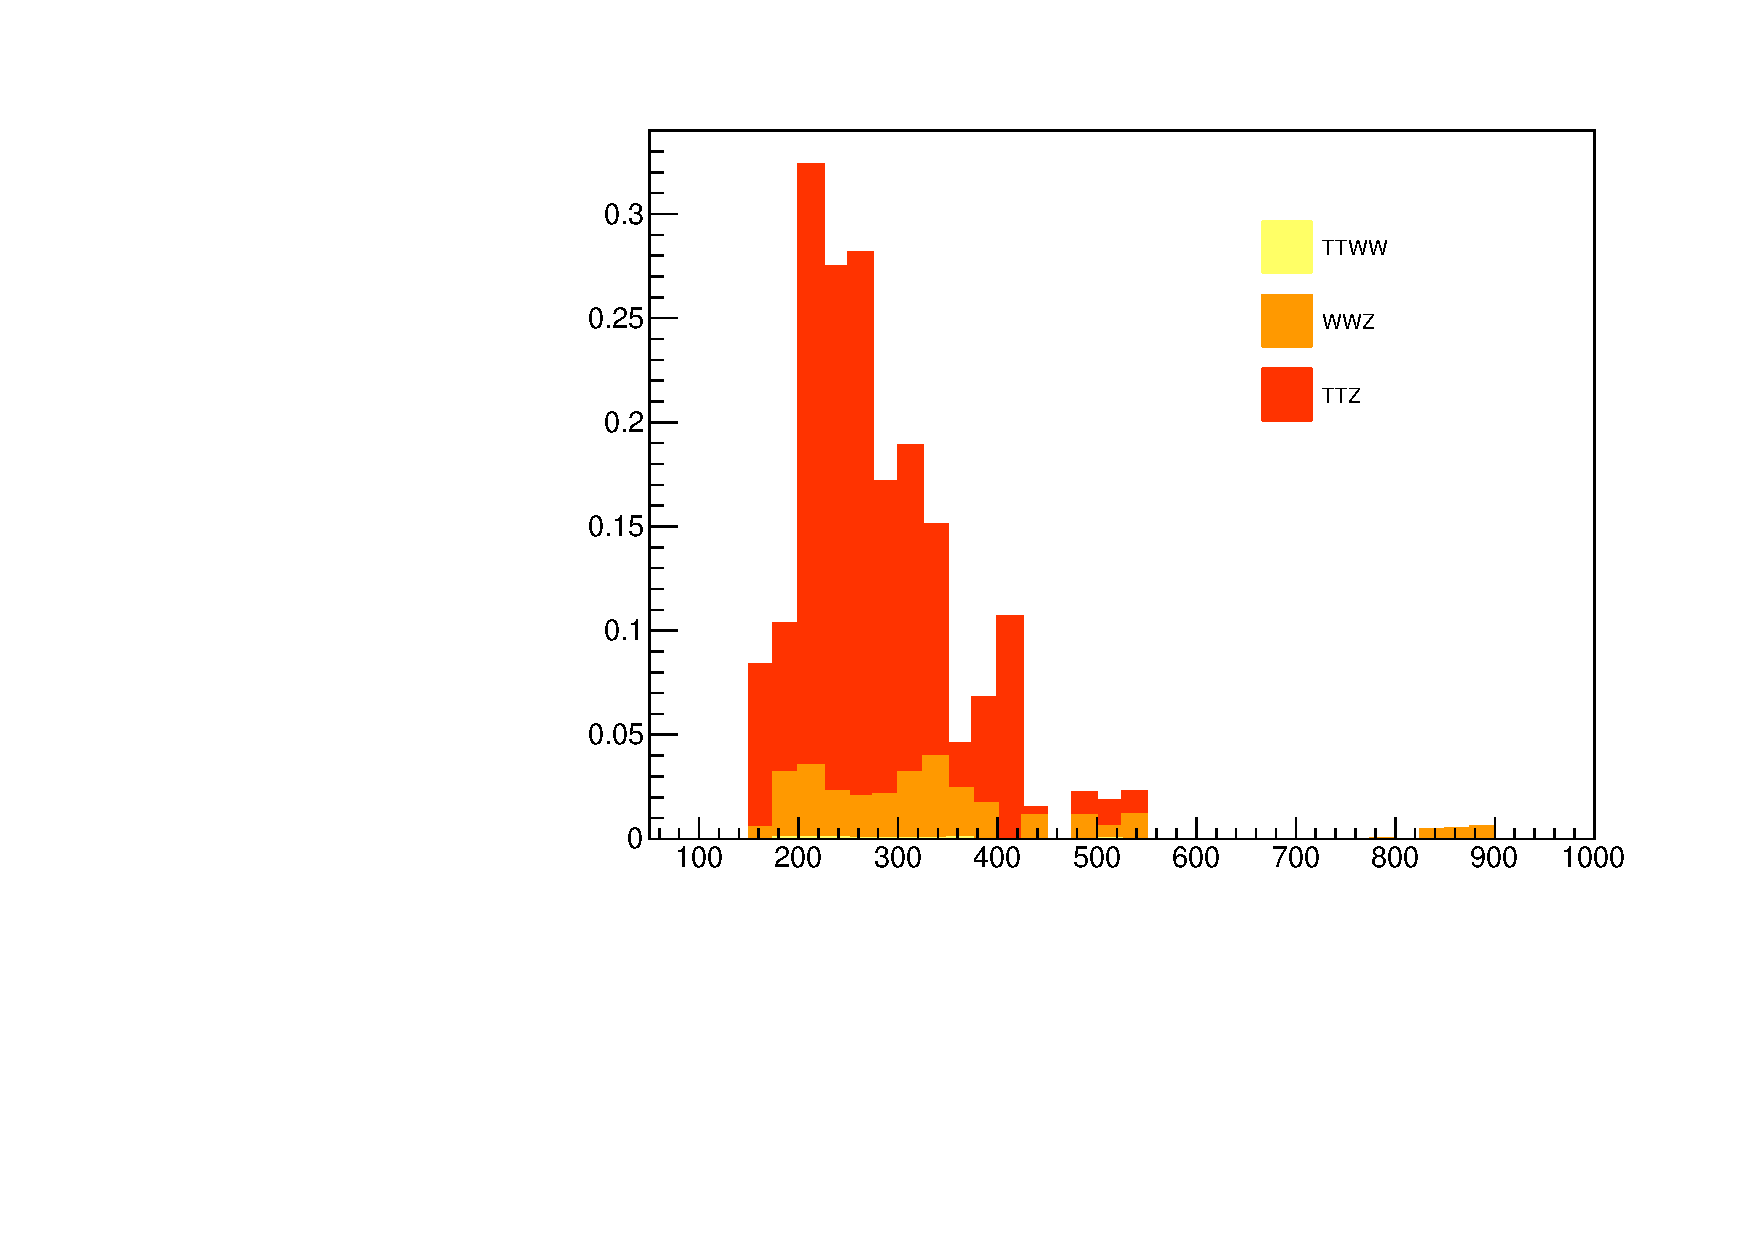
\includegraphics[width=\cmsFigWidth]{Figures/Mass_Irreducible_Bkg_MadGraphSet}
    %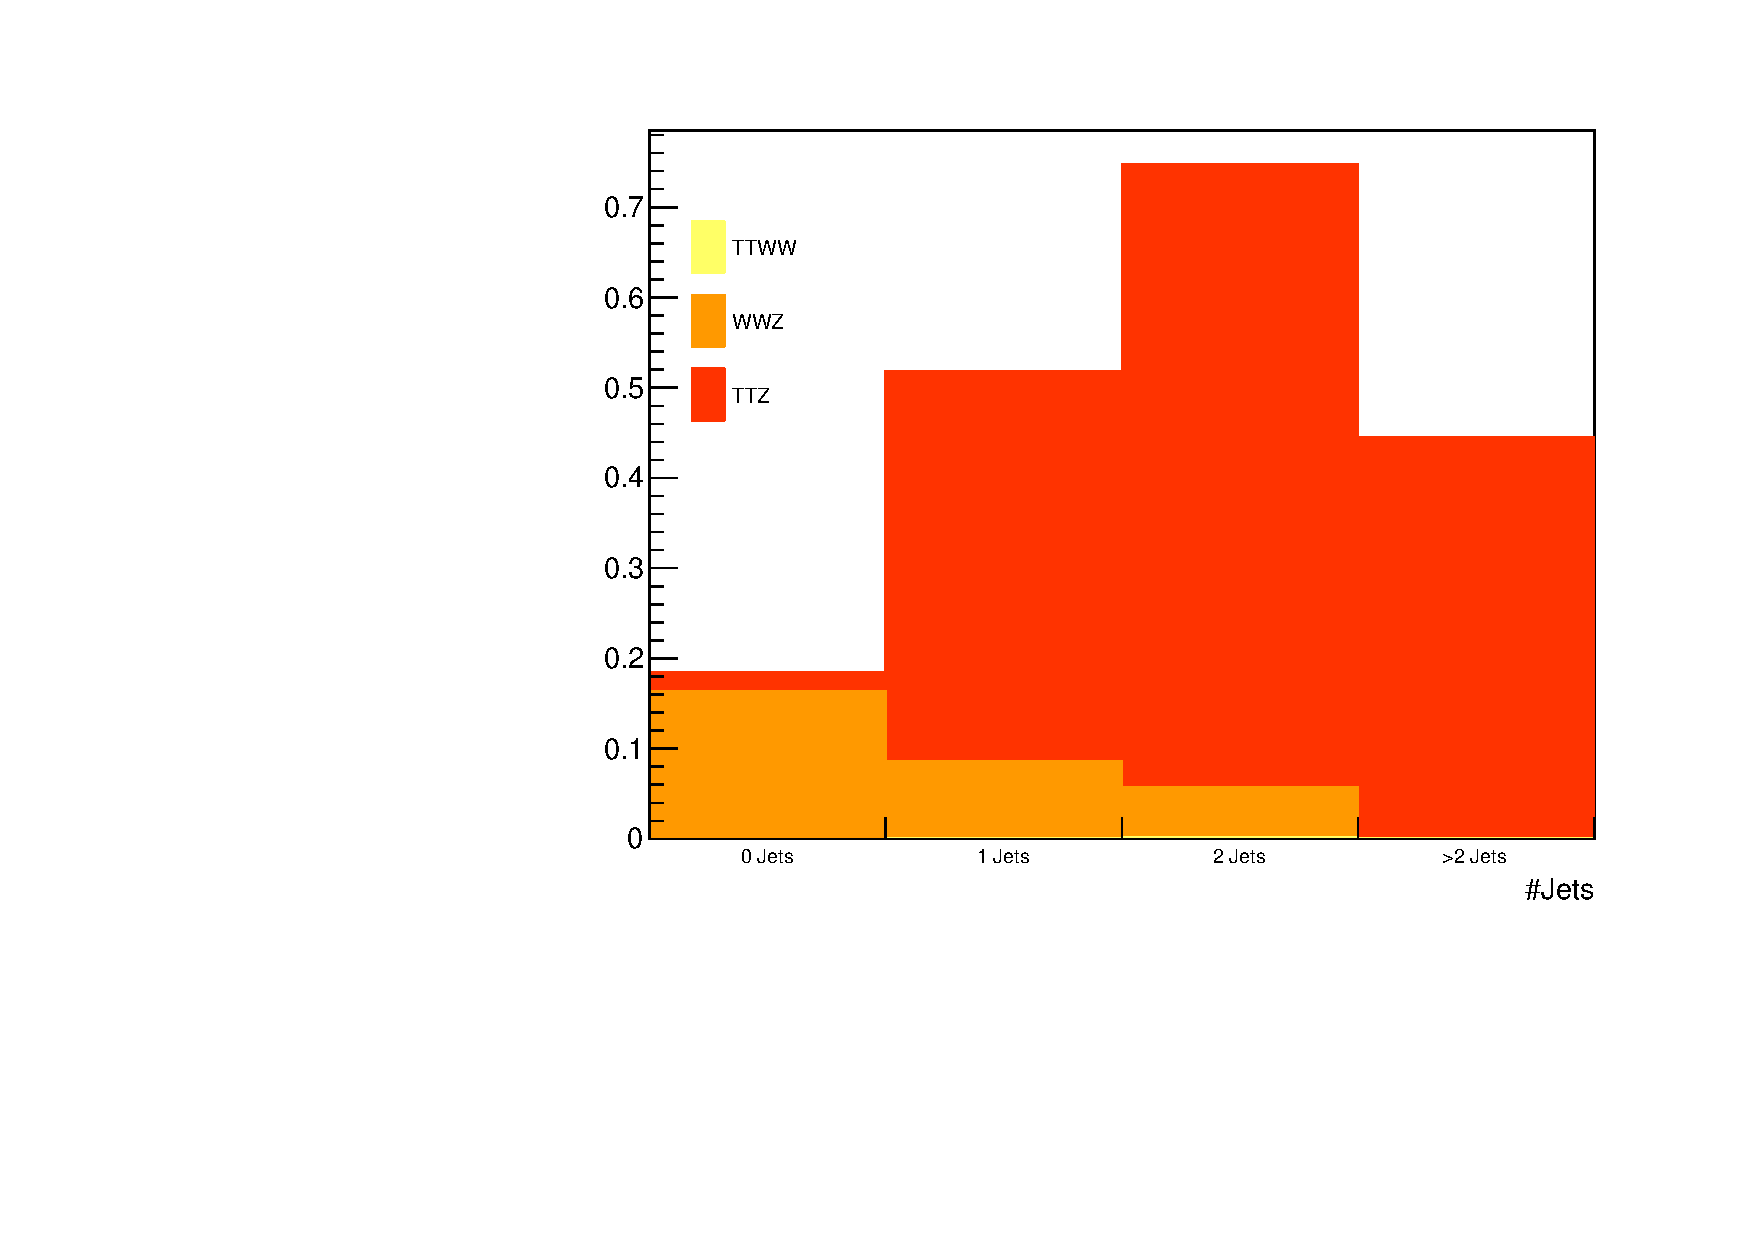
\includegraphics[width=\cmsFigWidth]{Figures/Jets_Irreducible_Bkg_MadGraphSet}
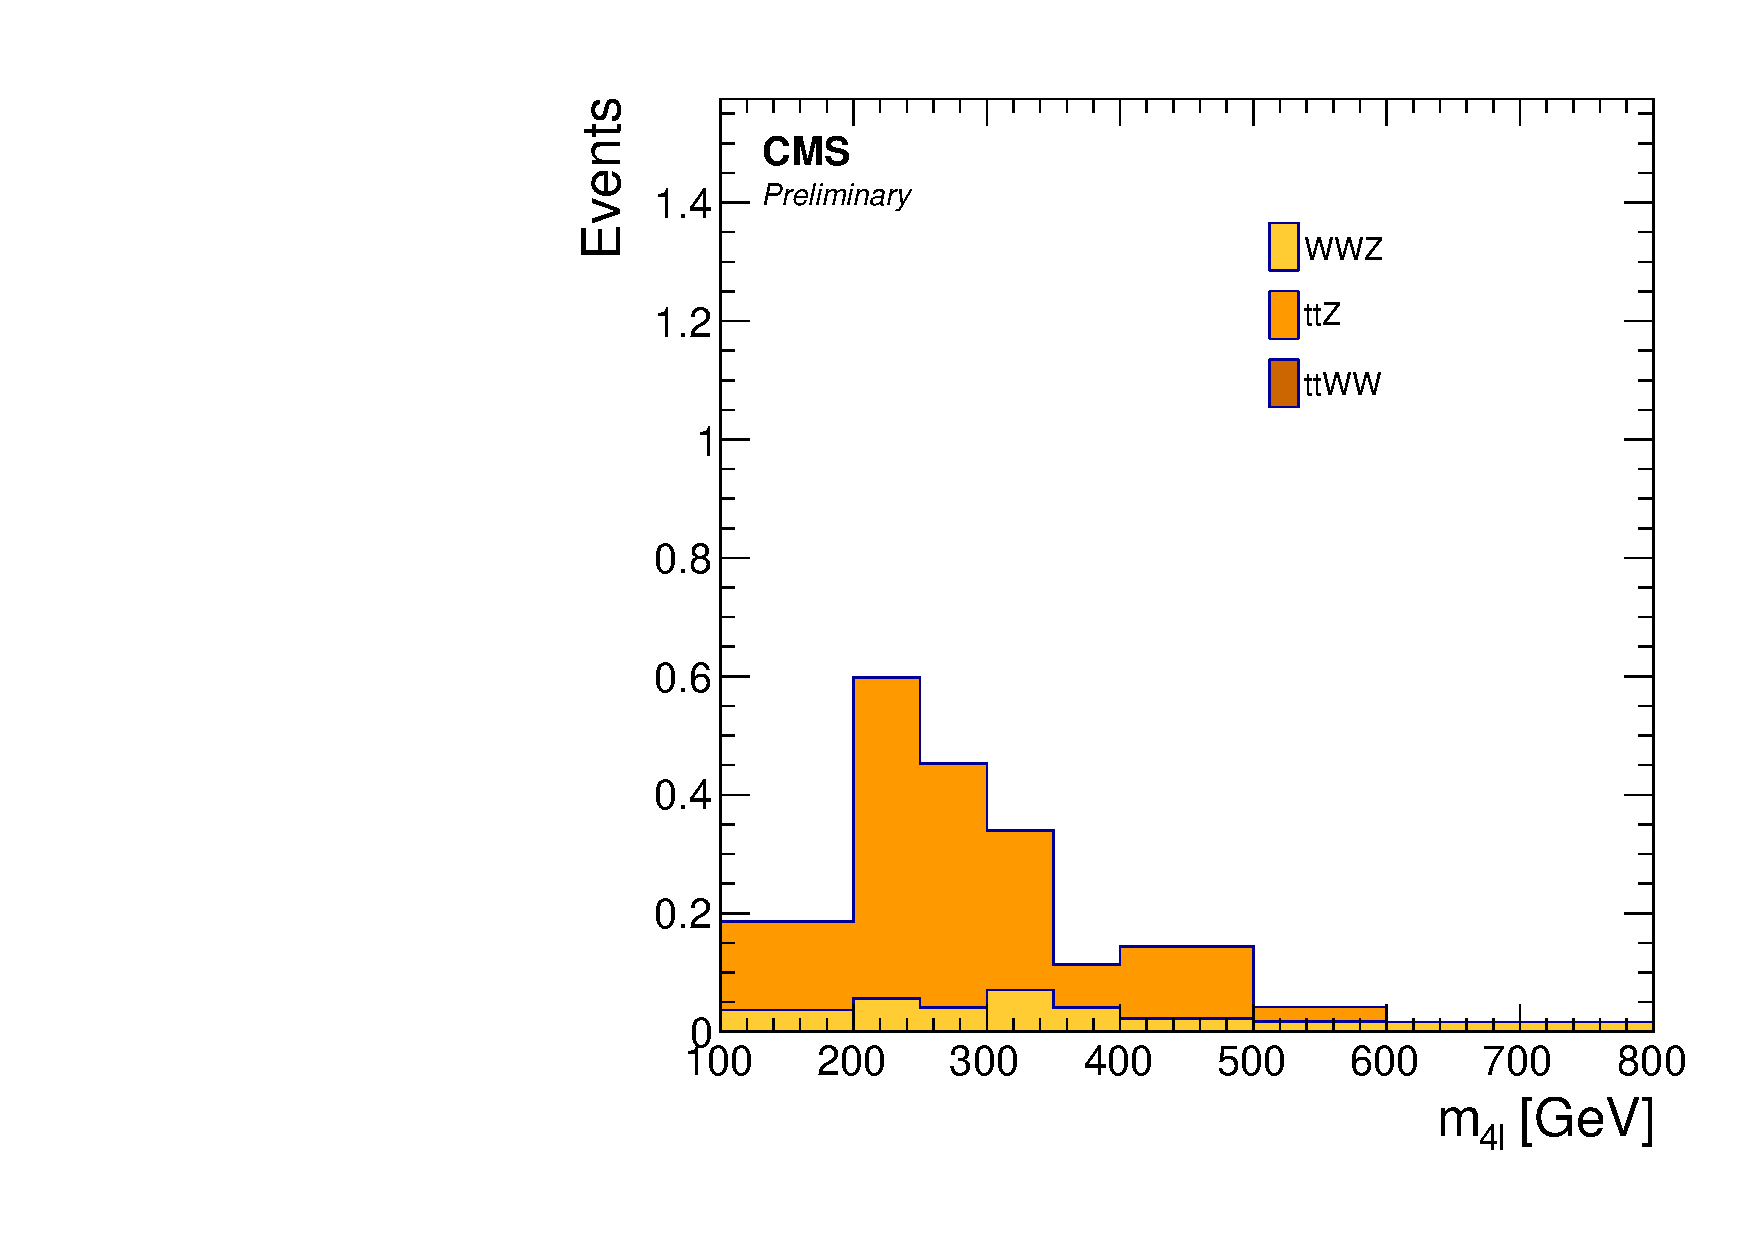
\includegraphics[width=\cmsFigWidth]{Figures/Mass_irr}
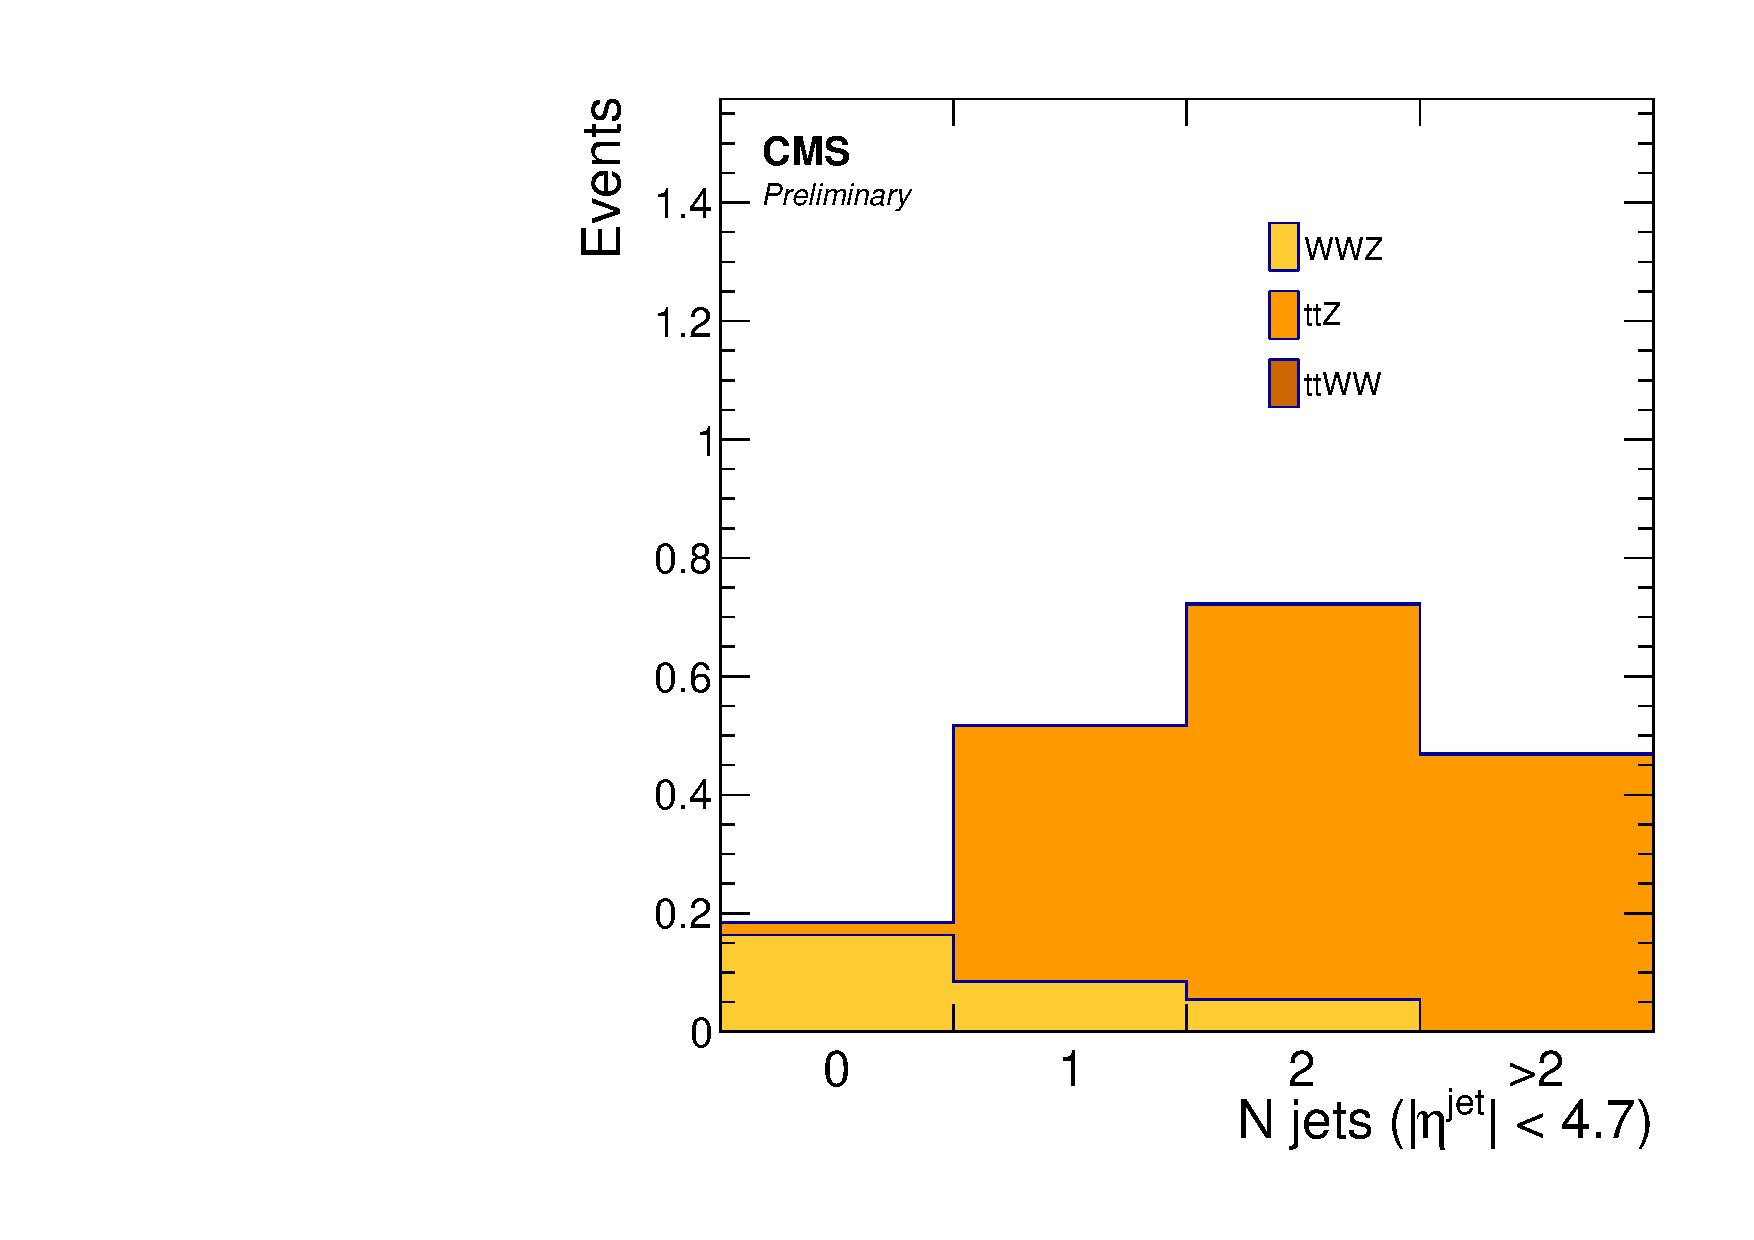
\includegraphics[width=\cmsFigWidth]{Figures/Jets_irr}
     \caption{Number of events of the irreducible background component in the signal region as a function of the invariant mass of the 4 lepton system (\cmsLeft) and the reconstructed number of jets produced in the event (\cmsRight).}
    \label{fig:irr_bkg}
  \end{center}
\end{figure}

The main background contribution that arises mostly from the $Z$ in association with jets, as well as from $t\bar{t}$, $WZ$ and
$WWW$ +jets, is estimated with data analyzed in dedicated control regions.
For this type of background, a jet or a non-prompt lepton (i.e. lepton produced in heavy meson decays) is misidentified as an isolated 
electron or muon. These processes are referred to as reducible background and are estimated using a data driven method, known
as ``method A'' in the $H\to ZZ \to 4\ell$ analysis~\cite{HiggsLegacyPaper}. This method is based on two control samples, obtained 
as subsets of four lepton events, by demanding a Z$_1$ candidate reconstructed with the same requirement as the  Z$_1$ built in the signal region, and two additional leptons, with opposite sign and same flavor ($e^\pm e^\mp$ or $\mu^\pm\mu^\mp$). The ``3P1F'' control sample contains events with only one of the two additional leptons failing identification and isolation 
criteria, the other being a good quality lepton, and it is used to estimate the contribution in the signal region of events with three genuine leptons, such as 
$WZ +$ jets.
In the ``2P2F'' control region, instead, the two additional leptons  are  both required  to  fail the final identification and isolation criteria. This  sample  is  meant  to  be  used  to  estimate  
both the  contribution  in  the  signal region and in the ``3P1F'' region of events with only two genuine leptons, such as Z + jets and $t\bar{t}$.  
The number of reducible background events in the signal region is given by the following formula:
\begin{equation}
\label{eq:redBkg_methA}
N^{red\ bkg}_{exp} = \sum_{i}^{N_{3P1F}} p_{i}- \sum_{i}^{N_{2P2F}} p_{i,1} p_{i,2},  
\end{equation}
where:
\begin{itemize}
\item $N_{3P1F}$ and $N_{2P2F}$ are the number of events in the ``3P1F'' and ``2P2F'' control regions respectively
\item $p_{i} = \frac{f_{i}}{1-f_{i}}$
\item $p_{i,1(2)} = \frac{f_{i,1(2)}}{1-f_{i,1(2)}}$
\item $f_{i}$  and $f_{i,1(2)}$ are the fake rates of the failing lepton in the ``3P1F'' sample and of the first (second) failing lepton in the ``2P2F'' control sample. 
\end{itemize}
The ``fake rate'' is the lepton misidentification probability $f(\pt^{\ell},\eta^{\ell})$
to extrapolate the background yields from the control region to the signal region. 
This probability is defined as the fraction of non-signal leptons passing the lepton selection of the analysis.
The fake rate is estimated in a sample composed by $Z_1 + 1\ell _{loose}$ events, 
where beside to the opposite sign/same flavor pair which forms the $Z_{1}$, 
exactly one additional lepton is reconstructed fulfilling all the selection requirements, 
but for the identification and the isolation cuts.\\
The lepton misidentification probability ranges from 1\% to 15\% and has a mild dependence on the pseudorapidities for the 
electrons.\\
In order to obtain the reducible background contribution as a function of the analyzed variables, the number of events in the ``3P1F'' and  ``2P2F'' 
control regions is estimated in each bin of each distribution separately, it is multiplied by the corresponding fake rate (depending on leptons $p_T$ and $\eta$) and summed, according to~\ref{eq:redBkg_methA}. In order to be consistent with the signal region, reconstructed jets that overlap with the loose leptons in the CRs are removed. In Figure~\ref{fig:red_bkg} the contribution of the reducible background is reported as a function of the 4-lepton invariant mass and the jet multiplicity, and it is estimated both from MC samples and by 
using the ``fake-rate'' method. The lack of statistics makes the data-driven estimate necessary.

\begin{figure}[hbtp]
  \begin{center}
   % 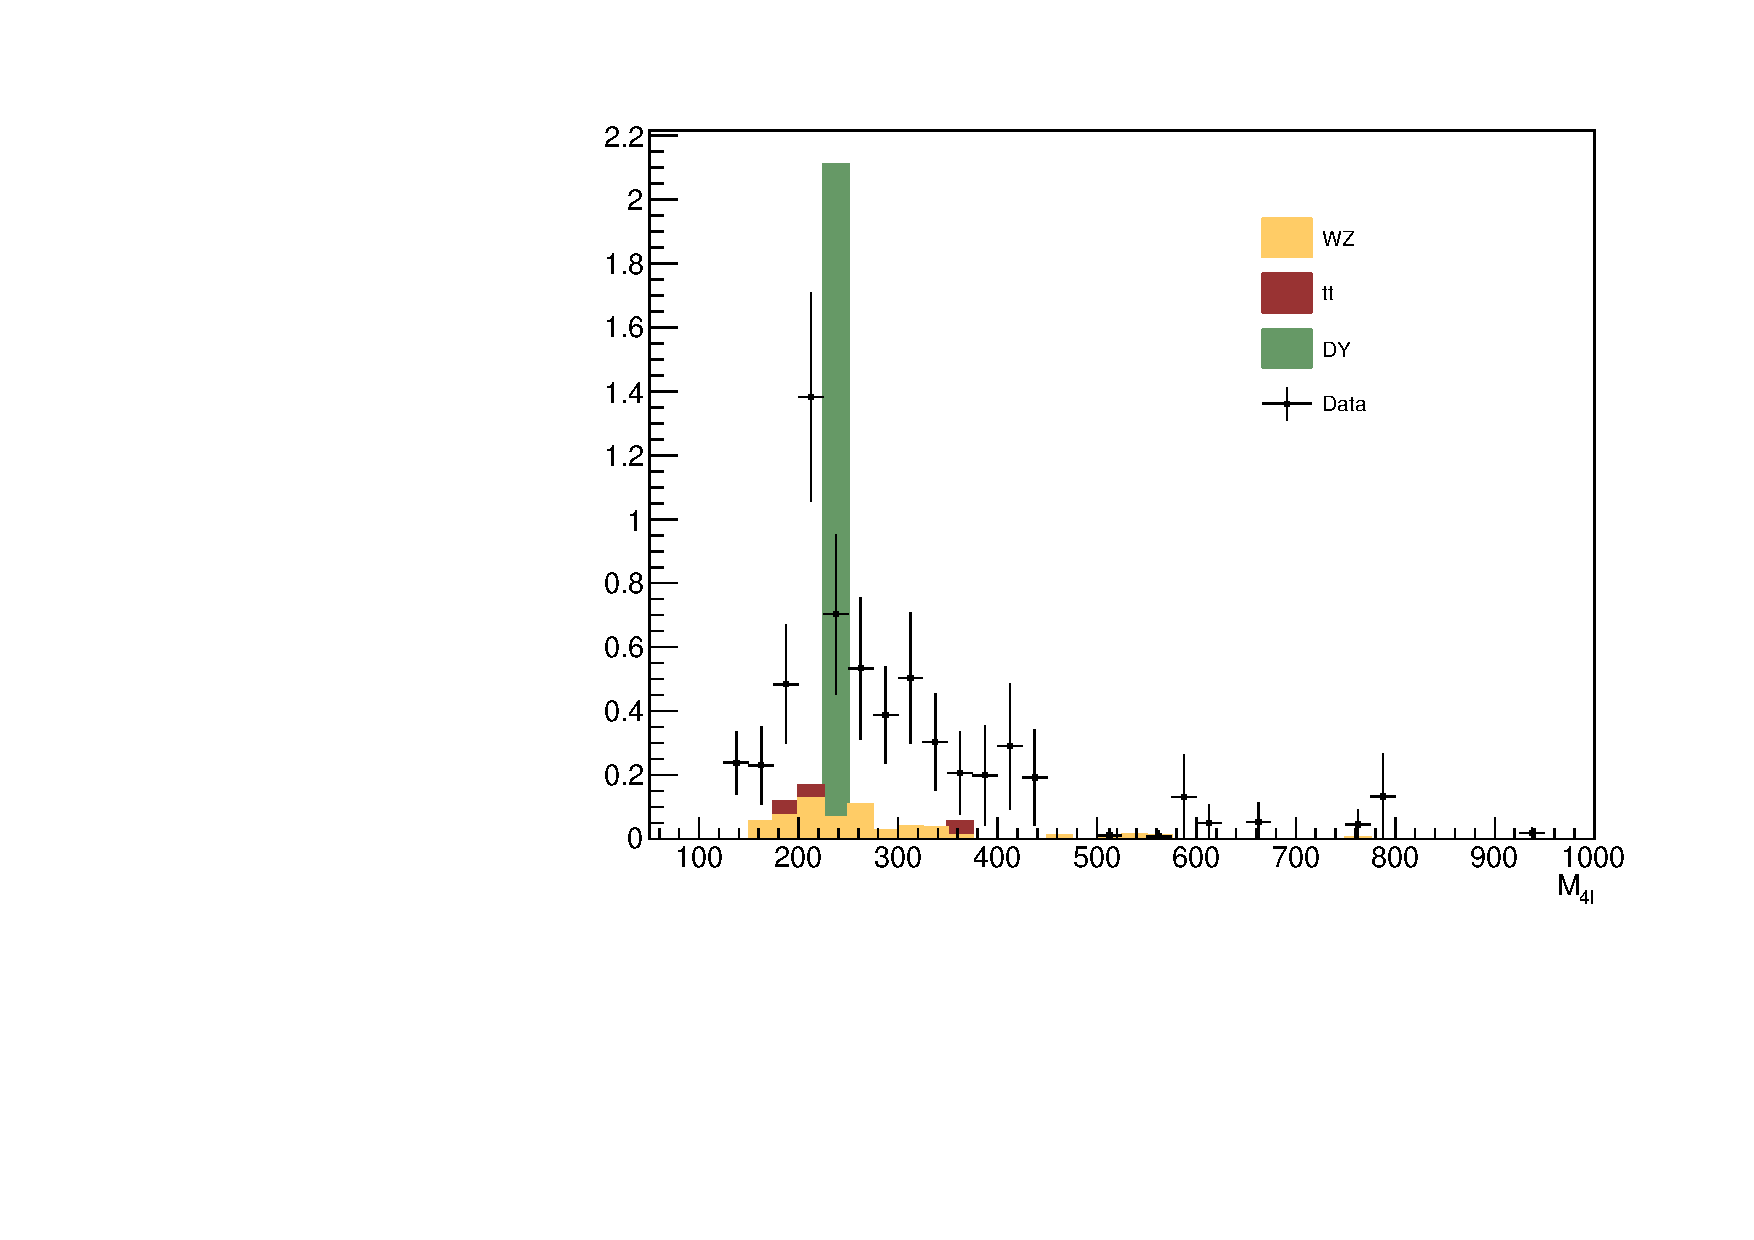
\includegraphics[width=\cmsFigWidth]{Figures/Mass_Reducible_Bkg_MadGraphSet}
    %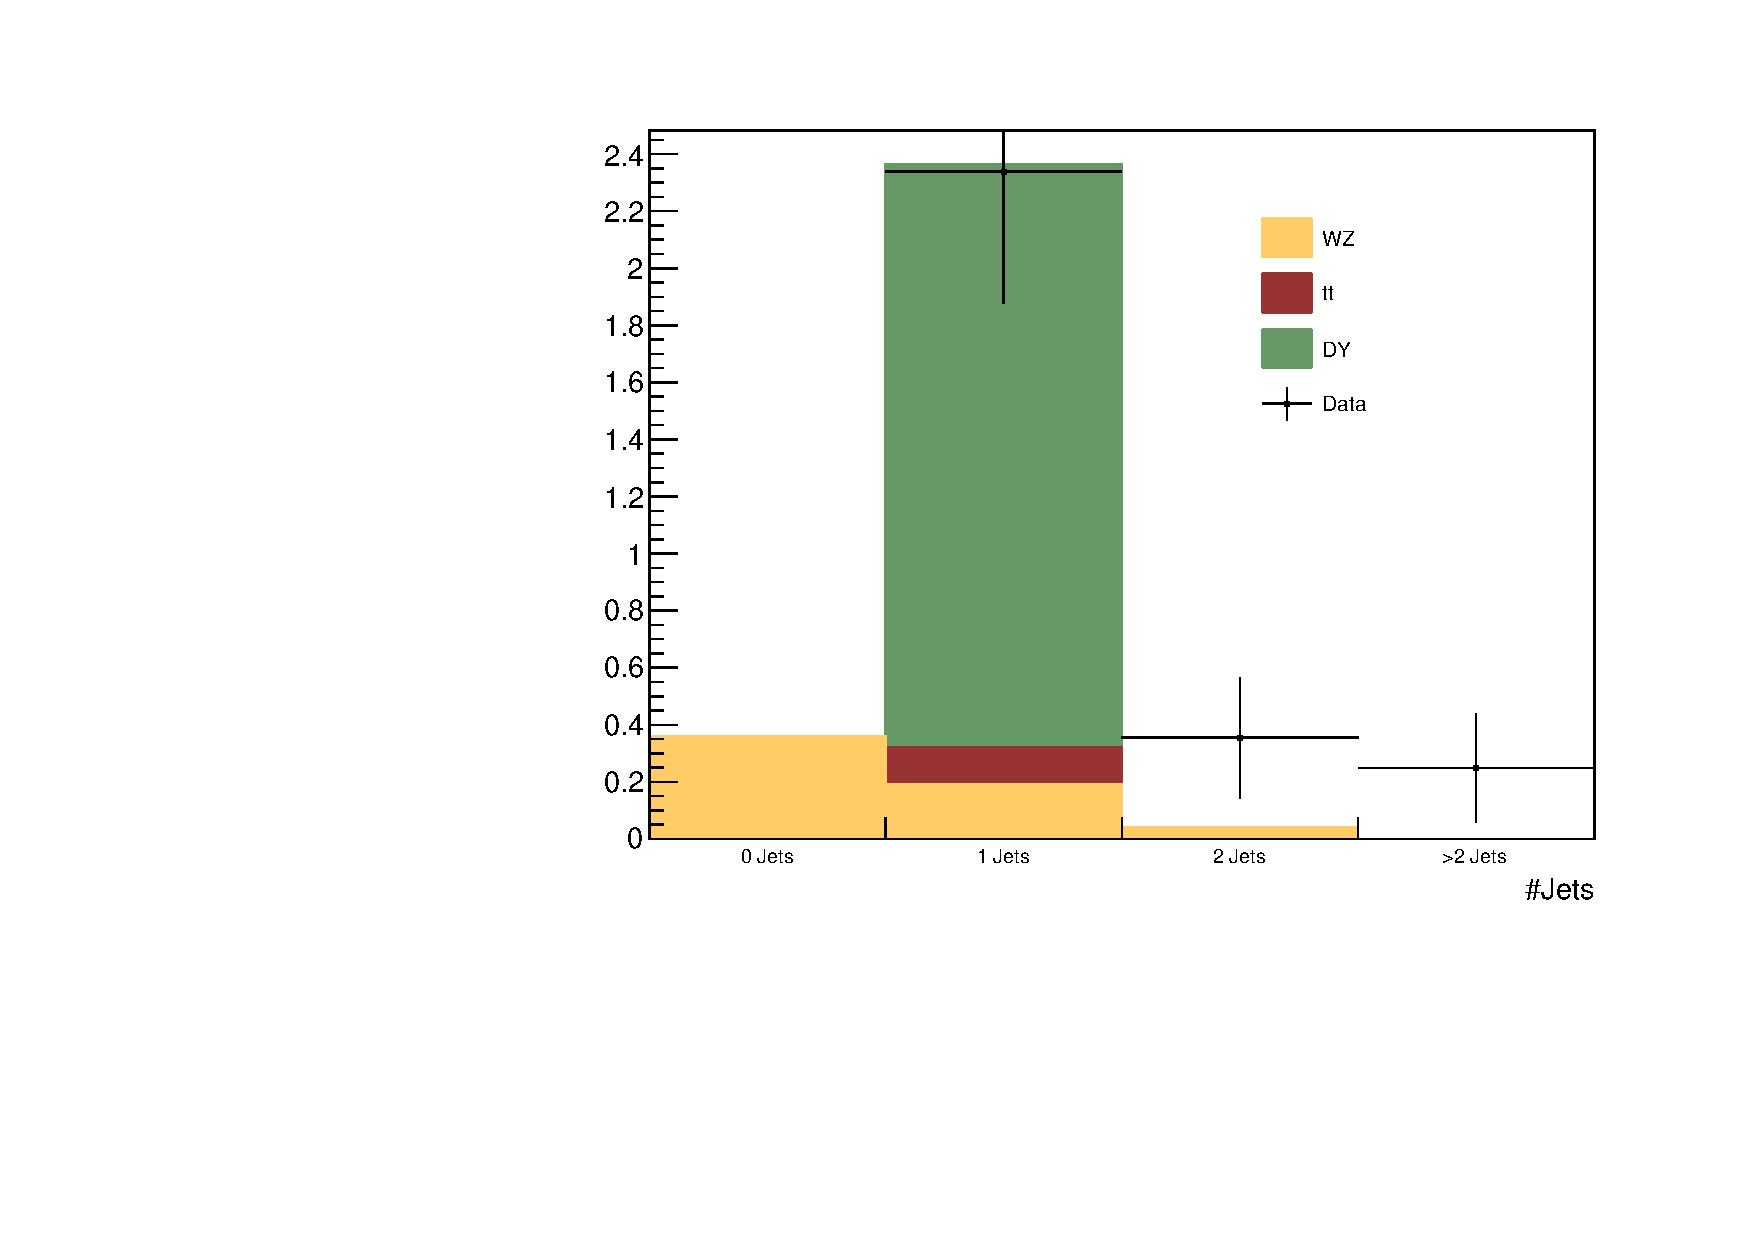
\includegraphics[width=\cmsFigWidth]{Figures/Jets_Reducible_Bkg_MadGraphSet}%FIXME 
    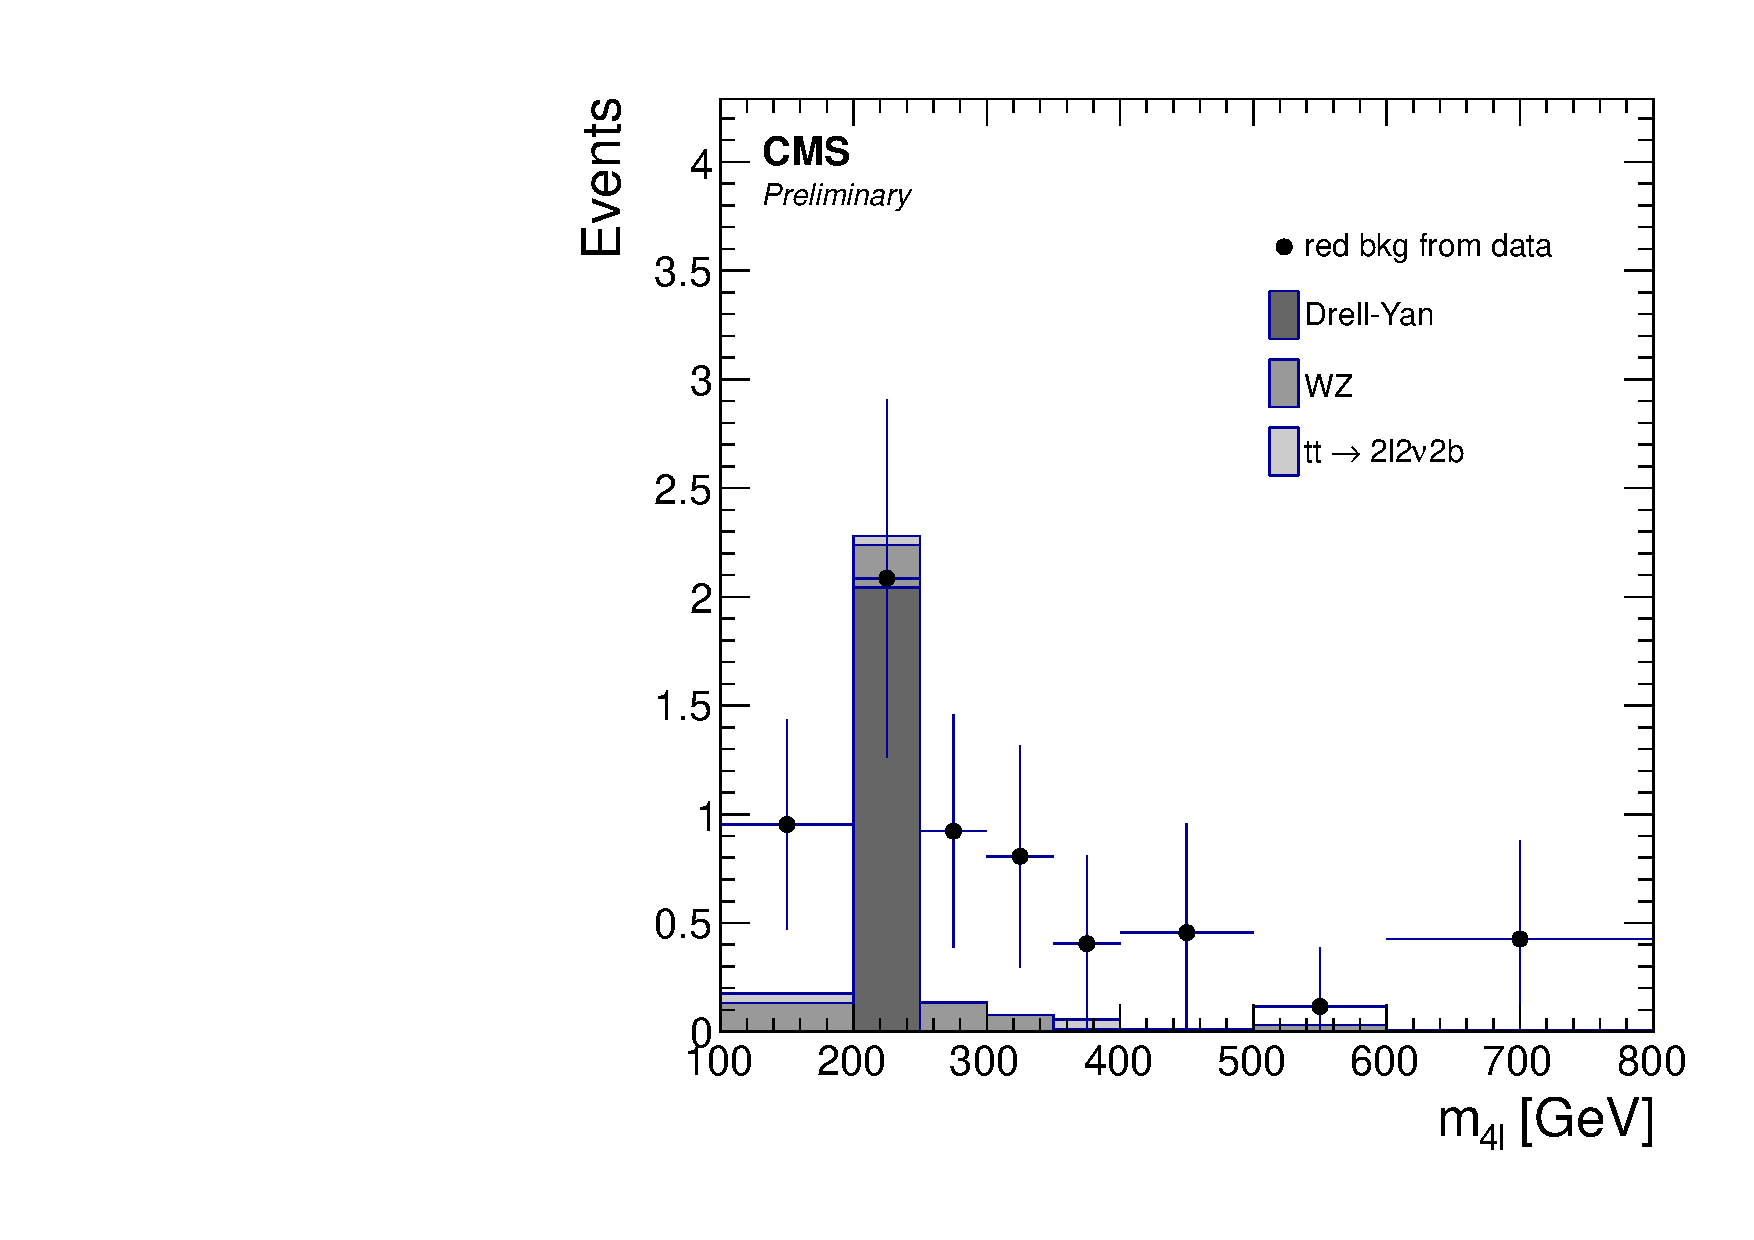
\includegraphics[width=\cmsFigWidth]{Figures/Mass_red}
    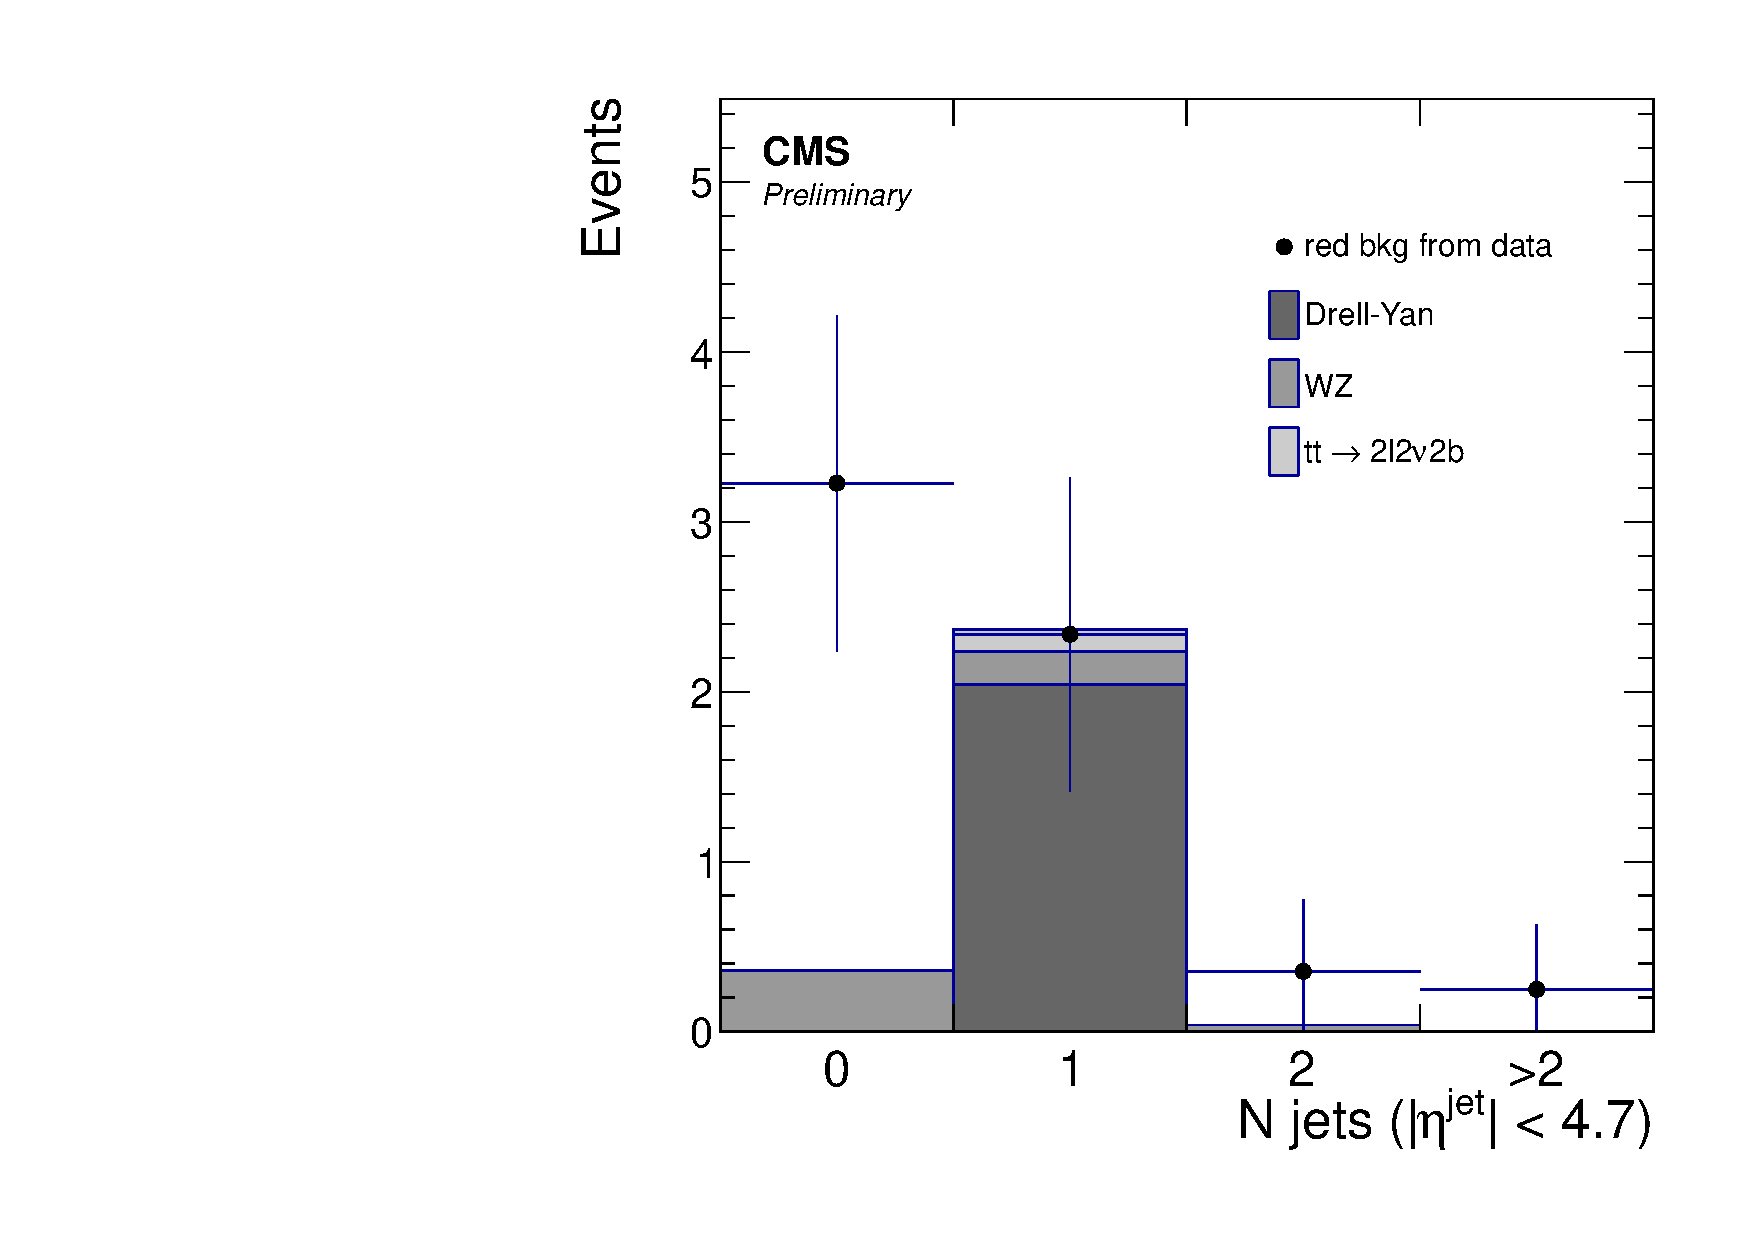
\includegraphics[width=\cmsFigWidth]{Figures/Jets_red}
     \caption{Reducible background component in the signal region as a function of the invariant mass of the 4 lepton system (\cmsLeft) and the reconstructed number of jets produced in the event (\cmsRight). Points represent the data-driven estimate, the stacked histogram represents the Monte Carlo predictions, characterized by a very poor statistics.}
    \label{fig:red_bkg}
  \end{center}
\end{figure}
%The reconstructed four-lepton invariant mass and the number of jets distributions are shown in Fig.~\ref{fig:sig_contr_Mad}.\\
%\begin{figure}[hbtp]
 % \begin{center}
  %  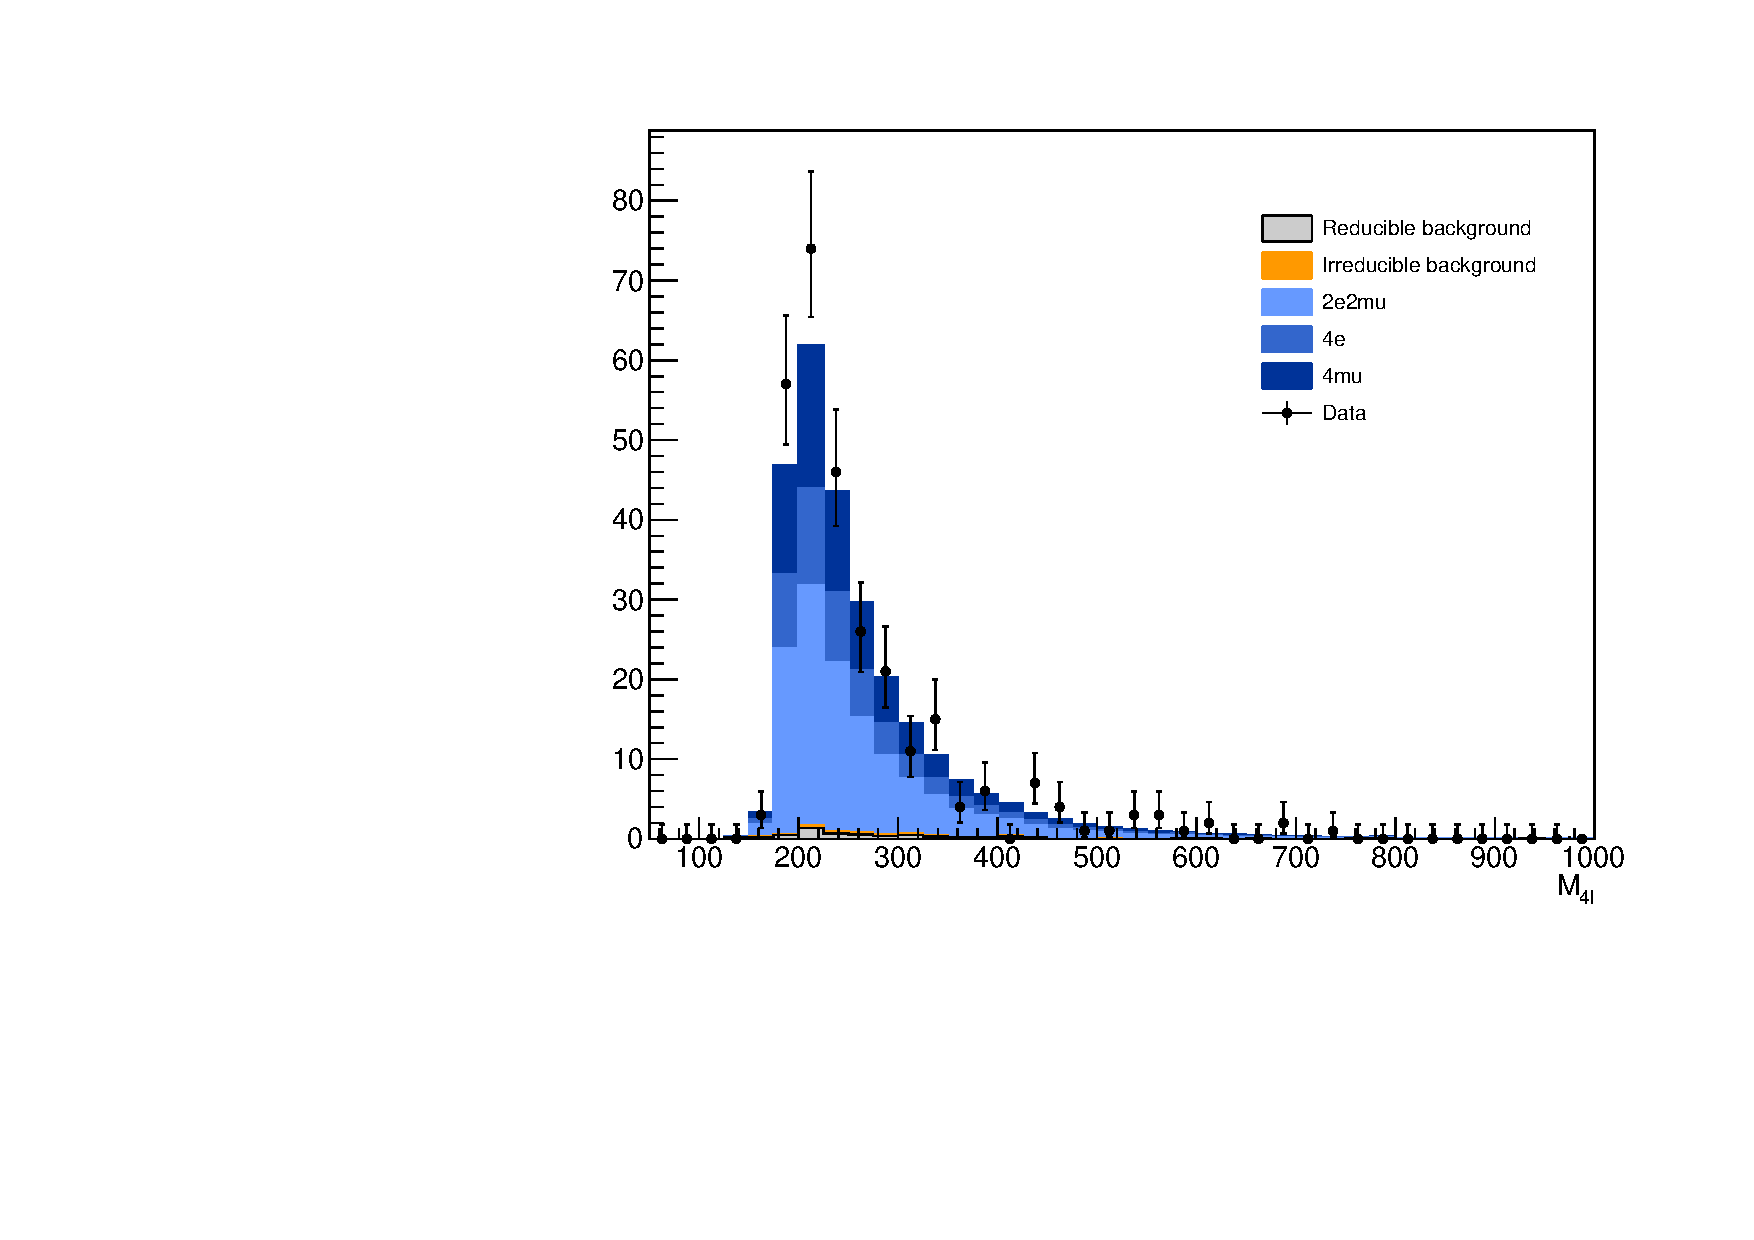
\includegraphics[width=\cmsFigWidth]{Figures/Mass_Final_State_MadGraphSet}
   % 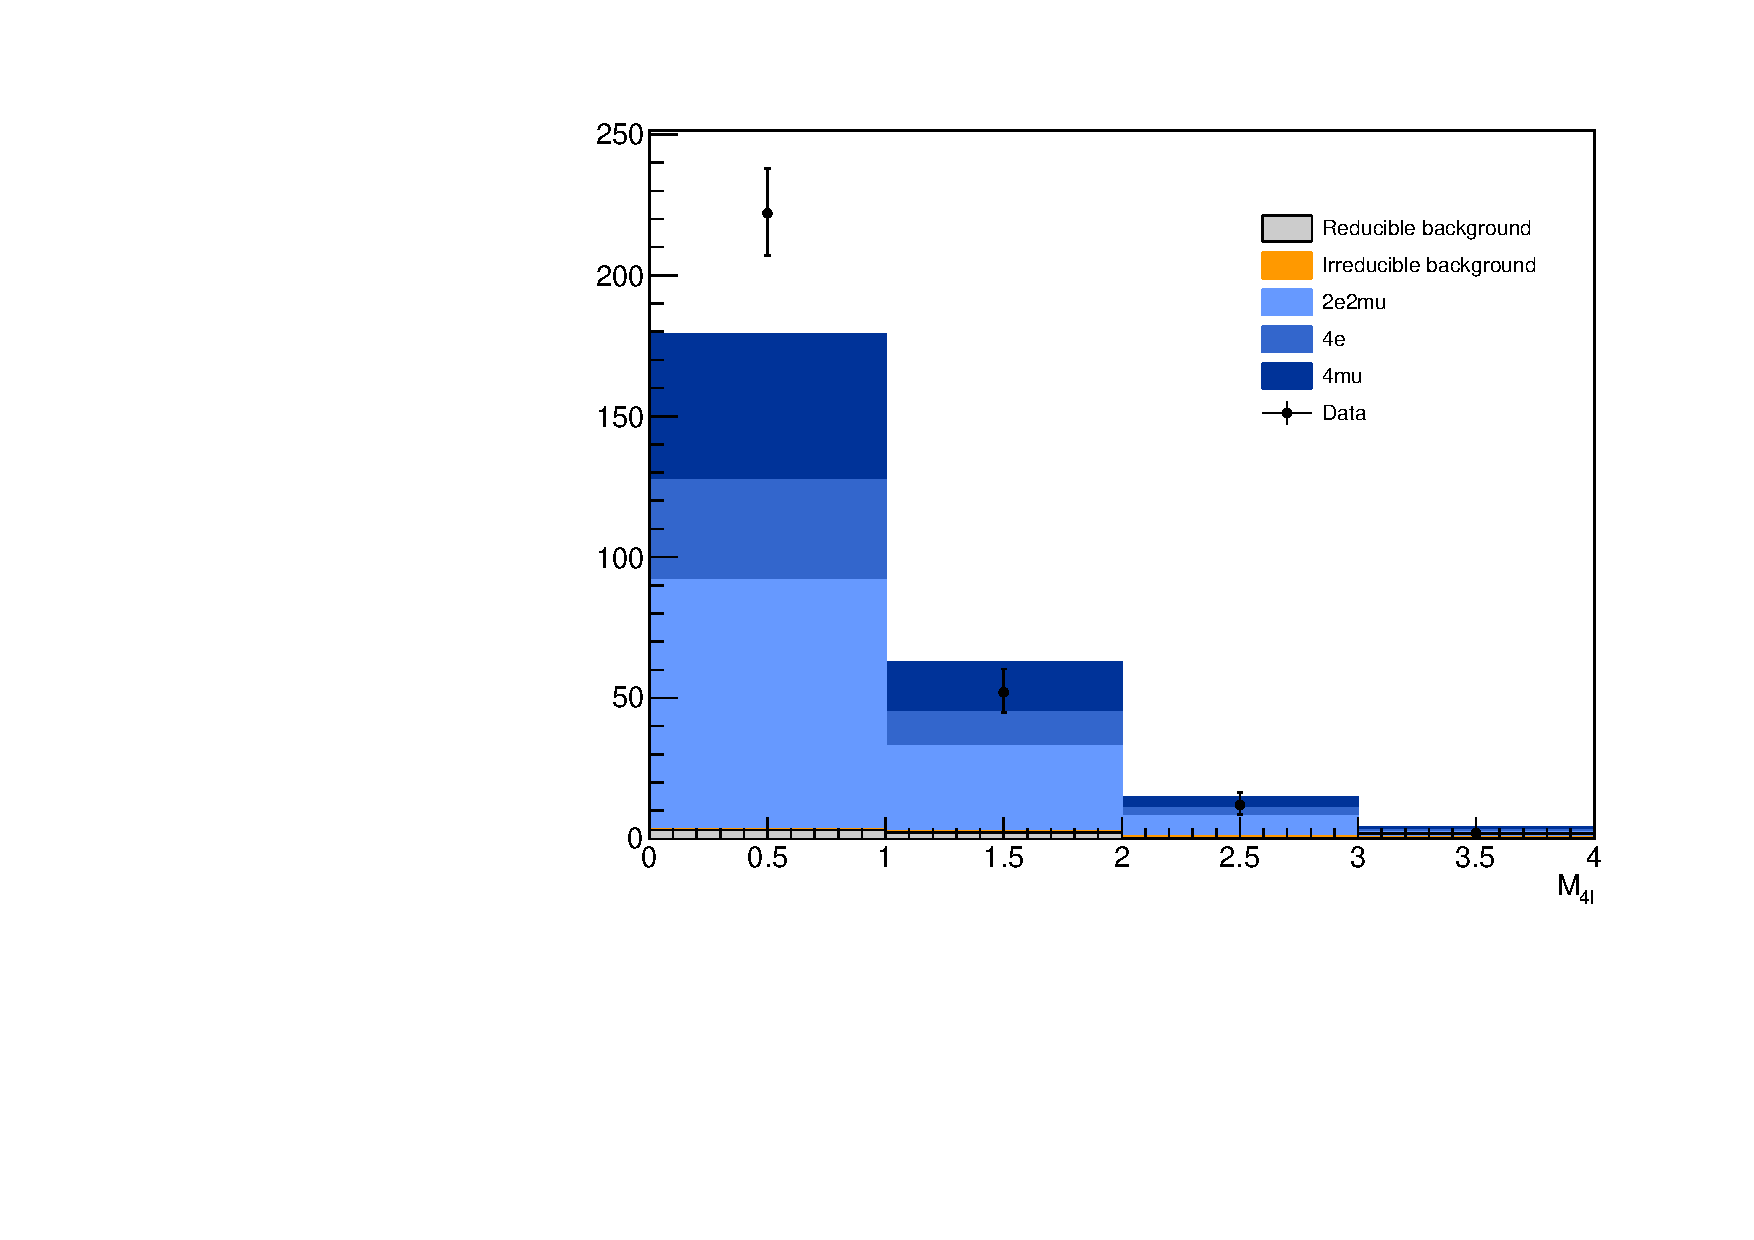
\includegraphics[width=\cmsFigWidth]{Figures/Jets_Final_State_MadGraphSet}
    % \caption{ Distribution of the reconstructed four-lepton mass (\cmsLeft). Distribution of the reconstructed number of jets produced in the event  (\cmsRight). Points represent the data, the stacked histogram represents the \texttt{MadGraph+MCFM+Phantom} predictions for $ZZ$ signal. The estimate of irreducible and reducible backgrounds is also reported.}
   % \label{fig:sig_contr_Mad}
 % \end{center}
%\end{figure}

%% --------------------------------------------------------- %%


%% --------------------------------------------------------- %%
\section{Systematic Uncertainties}
\label{sec:systunc}
%(The same as AN2013-134: check values!! FIXME)\\
\label{sec:systunc}
Systematic uncertainties for trigger efficiency (1.5\%) are evaluated from data~\cite{ZZXSPaper}. Uncertainties
arising from lepton identification, isolation, tracking and impact parameter are 1-5\% for muons and electrons~\cite{ZZXSPaper}. The uncertainty in the LHC integrated
luminosity of the data sample is 2.6\%~\cite{CMS-PAS-LUM-13-001}. Theoretical uncertainties in the $ZZ \to \ell\ell\ell'\ell'$ 
acceptance are evaluated using \texttt{MCFM} and by varying the renormalization and factorization scales, up and down, 
by a factor of two with respect to the default values $\mu_R = \mu_F = m_Z$. The variations in the acceptance are 0.1\% (NLO
$q\bar{q} \to ZZ$) and 0.4\% ($gg \to ZZ$), and can be neglected. Uncertainties related to the choice
of the PDF and the strong coupling constant are evaluated following the \texttt{PDF4LHC} ~\cite{PDF4LHCRec, PDF4LHCRep, CT10} prescription and 
using \texttt{CT10},  \texttt{MSTW08}, and  \texttt{NNPDF}~\cite{NNPDF} PDF sets. They are found to be 1.2\% in the wider fiducial region and 0.8\% in the tighter fiducial region (fiducial regions are defined in the next section).
%4\% (NLO $q\bar{q} \to ZZ$) and 5\% ($gg \to ZZ$)~\cite{ZZXSPaper}.

The reducible background uncertainties in $Z$ + jets, $WZ$ + jets and $t\bar{t}$ yields reflect the uncertainties in the measured values of the misidentification rates and the limited statistics of the control regions in the data, and vary between 30\% and 70\% on the background yield, which corresponds to a $\sim$1\% of uncertainty on the cross-section measurement. The irreducible background uncertainty is smaller and varies between 13\% and 26\% on the yield (less than 1\% on the cross-section estimate). Table~\ref{tab:syst} summarizes the sources  of systematic uncertainty and their values.

\begin{table*}[htbH]
\begin{center}
\topcaption{Estimated systematic uncertainties on the signal yield used to compute the inclusive cross section measurement\label{tab:syst}}
\begin{tabular}{lclc}
\hline Systematic source & Uncertainty value\\
\hline Trigger & 1.5\%  \\
Lepton ID, ISO and Tracking & 1-5\%\\
Luminosity & 2.6\%\\
Reducible background & $\sim$1\%\\
Irreducible background & $<$1\%\\
Acceptance for PDF & 0.8-1.2\%\\
\hline
\end{tabular}
\end{center}
\end{table*}

% The uncertainty in the unfolding procedure discussed in Section 7 arises from differences between
% SHERPA and POWHEG for the unfolding factors (2–3%), from scale and PDF uncertainties
% (4–5%), and from experimental uncertainties (4–5%).


%% --------------------------------------------------------- %%



%% --------------------------------------------------------- %%
\section{Results}
\label{sec:results}
\subsection{Inclusive ZZ cross section measurement}

The inclusive cross-section is determined as 
$$\sigma_{pp\to ZZ} = \frac{N_{data}-N_{bkg}}{\mathcal{L}\cdot A \cdot \epsilon \cdot \mathcal{B}(Z\to \ell^+\ell^-)\cdot\mathcal{B}(Z\to \ell'^+\ell'^-)},$$
where $N_{data}$ and $N_{bkg}$ are the total number of data and background events, $A$ is the geometrical acceptance, $\epsilon$ is the signal efficiency, $\mathcal{L} = 19.7$ fb$^{-1}$ is the integrated luminosity and $\mathcal{B}(Z\to \ell^+\ell^-) = 3.363 \pm 0.004$ ($3.366\pm 0.007$)\% is the branching fraction of a $Z$ boson decaying into an electron (muon) pair~\cite{PDG}.

The region in which the measurement is performed (called ``fiducial region'') is defined by requiring the invariant mass of each Z boson 
between 60 and 120 GeV. % and the invariant mass of the Z-boson pair ($m_{ZZ}$) above 100 GeV. 
The product of acceptance and efficiency ($A\cdot\epsilon$) is evaluated from simulation and defined as the ratio between the
number of events in the fiducial region that pass the analysis selection at reconstruction level and the number of events generated in that
fiducial region. 
%sum of $q\bar{q} \to ZZ$ and  $gg \to ZZ$ generated events, with $Z\to \ell^+\ell^-$, and the events accepted by the analysis
%selection at reconstructed level corrected for each individual lepton flavor in bins of pT and h using factors obtained with the ``tag-and-probe'' technique. 
The requirements on $p_T$ and $\eta$ for the particles in the final state reduce the full possible phase space of the $ZZ \to 4
\ell$ measurement by a factor within a range of 0.32-0.47 for the $4e$, $4\mu$ and $2e2\mu$ (depending on
the final state) with respect to all events generated in the mass window $60 < m_{Z_1} ,m_{Z_2} < 120$ GeV.
The $A\cdot\epsilon$ product estimated for each final state and for the different samples is listed in 
Tables~\ref{tab:Aeps_tot} and ~\ref{tab:Aeps_samples}.

%\begin{table*}[htbH]
%\begin{center}
%\caption{Selection efficiency and $A\cdot \epsilon$ product for the three final states used in the $pp\to ZZ$ cross-section measurement.
%%The values reported are a product of the detector geometrical acceptance and the object reconstruction and event identification efficiency.
%}
% \label{tab:Aeps_tot}
%\begin{tabular}{ccc}
%\hline Final State & $\epsilon$ & $A\cdot\epsilon$\\
%\hline $4\mu$ & 84\%& 47\%  \\
%$4e$ & 55\%& 32\%\\
%$2e2\mu$ &69\%& 40\%\\
%\hline
%\end{tabular}
%\end{center}
%\end{table*}

\begin{table*}[htbH]
\begin{center}
\topcaption{$A\cdot \epsilon$ for the three final states used in the $pp\to ZZ$ cross-section measurement.
The values reported are a product of the detector geometrical acceptance and
the object reconstruction and event identification efficiency. \label{tab:Aeps_tot}}
\begin{tabular}{cc}
\hline Final State & $A\cdot\epsilon$\\
\hline $4\mu$ & 47\%  \\
$4e$ & 32\%\\
$2e2\mu$ & 40\%\\
\hline
\end{tabular}
\end{center}
\end{table*}

\begin{table*}[htbH]
\begin{center}
\caption{Signal yield and efficiency for the signal samples.
The $A\cdot\epsilon$ values reported are a product of the detector geometrical acceptance and
the object reconstruction and event identification efficiency.}
 \label{tab:Aeps_samples}
\begin{tabular}{lcccccc}
\hline  \multicolumn{1}{c}{Process} & \multicolumn{3}{c}{Signal yield} & \multicolumn{3}{c}{$A\cdot\epsilon$}\\
\hline  & $2e2\mu$ & $4e$& $4\mu$ & $2e2\mu$ & $4e$ &$4\mu$\\ 
\hline $ZZ\to 4\ell$ (\texttt{MadGraph}) & 125.3& 51.7 &51.7 &0.39 & 0.32& 0.46  \\
 $q\bar{q}\to ZZ\to 4\mu$  (\texttt{Powheg})& - & - & 69.6 & - & - & 0.46\\
$q\bar{q}\to ZZ\to 4e$  (\texttt{Powheg}) & - & 48.0 & - & - & 0.32 & -\\
$q\bar{q} \to ZZ\to 2e2\mu$  (\texttt{Powheg}) & 117.6 & - & - & 0.39 & - & -\\
$gg\to ZZ\to 4\mu$  (\texttt{MCFM})& - & - & 5.04& - & - & 0.72\\
$gg\to ZZ\to 4e$  (\texttt{MCFM}) & - & 3.47 & - & - & 0.49 & -\\
$gg\to ZZ\to 2e2\mu$  (\texttt{MCFM})& 8.52 & - & - & 0.60 & - & -\\
$ZZ\to 4\mu +2jets$  (\texttt{Phantom})& - & - & 0.633 & - & - & 0.65\\
$ZZ\to 4e +2jets$  (\texttt{Phantom})& - & 0.440 & - & 0.45 &-\\
$ZZ\to 2e2\mu +2jets$  (\texttt{Phantom})& 1.08 & - & - & 0.56 & - & -\\
$ZZZ + jets$ (\texttt{MadGraph}) & 0.284 & 0.121 & 0.192 & 0.42 & 0.35 & 0.54\\
$WZZ + jets$ (\texttt{MadGraph}) & 0.328 & 0.138 & 0.239 & 0.44 & 0.33 & 0.49\\
$W + H$ (\texttt{MadGraph})& 0.015 & 0.0058 & 0.0092 & 0.40 & 0.35 & 0.53\\
$Z + H$( \texttt{MadGraph}) & 0.200 & 0.083 & 0.117 & 0.42 & 0.34 & 0.48\\
$t\bar{t}+H$ (\texttt{MadGraph})& 0.017 & 0.007 & 0.010 & 0.44 & 0.34 & 0.49\\
\hline
\textbf{Total MadGraph Set} & \textbf{135.78} &\textbf{55.93} &\textbf{80.64} & \textbf{0.40} & \textbf{0.32} & \textbf{0.47}\\
\textbf{Total Powheg Set} & \textbf{128.25} &\textbf{52.33} &\textbf{75.89} & \textbf{0.40} & \textbf{0.32} & \textbf{0.47}\\
 \hline
\end{tabular}
\end{center}
\end{table*}
%\begin{table*}[htbH]
%\begin{center}
%\topcaption{Signal yield and efficiency for the signal samples.
%The $A\cdot\epsilon$ values reported are a product of the detector geometrical acceptance and
%the object reconstruction and event identification efficiency. \label{tab:Aeps_samples}}
%\begin{tabular}{lcccccc}
%\hline  \multicolumn{1}{c}{Process} & \multicolumn{3}{c}{Signal yield} & \multicolumn{3}{c}{$A\cdot\epsilon$}\\
%\hline  & $2e2\mu$ & $4\mu$& $4e$ & $2e2\mu$ & $4\mu$ &$4e$\\ 
%\hline $ZZ\to 4\ell$ (\texttt{MadGraph}) & 125.338& 51.67054 &51.67054 &0.39 & 0.32& 0.46  \\
% $q\bar{q}\to ZZ\to 4\mu$  (\texttt{Powheg})& - & - & 69.577 & - & - & 0.46\\
%$q\bar{q}\to ZZ\to 4e$  (\texttt{Powheg}) & - & 48.012 & - & - & 0.32 & -\\
%$q\bar{q} \to ZZ\to 2e2\mu$  (\texttt{Powheg}) & 117.637 & - & - & 0.39 & - & -\\
%$gg\to ZZ\to 4\mu$  (\texttt{MCFM})& - & - & 5.03656466 & - & - & 0.72\\
%$gg\to ZZ\to 4e$  (\texttt{MCFM}) & - & 3.46719 & - & - & 0.49 & -\\
%$gg\to ZZ\to 2e2\mu$  (\texttt{MCFM})& 8.519 & - & - & 0.60 & - & -\\
%$ZZ\to 4\mu +2jets$  (\texttt{Phantom})& - & - & 0.632893 & - & - & 0.65\\
%$ZZ\to 4e +2jets$  (\texttt{Phantom})& - & 0.439676 & - & 0.45 &-\\
%$ZZ\to 2e2\mu +2jets$  (\texttt{Phantom})& 1.076 & - & - & 0.56 & - & -\\
%$ZZZ + jets$ (\texttt{MadGraph}) & 0.283865 & 0.120920 & 0.191878 & 0.42 & 0.35 & 0.54\\
%$WZZ + jets$ (\texttt{MadGraph}) & 0.328 & 0.13792 & 0.23904576 & 0.44 & 0.33 & 0.49\\
%$W + H$ (\texttt{MadGraph})& 0.015 & 0.0057715 & 0.0092137 & 0.40 & 0.35 & 0.53\\
%$Z + H$( \texttt{MadGraph}) & 0.200 & 0.08323 & 0.116719 & 0.42 & 0.34 & 0.48\\
%$t\bar{t}+H$ (\texttt{MadGraph})& 0.017 & 0.007473 & 0.009666 & 0.44 & 0.34 & 0.49\\
%\hline
%\textbf{Total MadGraph Set} & \textbf{135.775} &\textbf{55.933} &\textbf{80.640} & \textbf{0.40} & \textbf{0.32} & \textbf{0.47}\\
%\textbf{Total Powheg Set} & \textbf{128.25} &\textbf{52.33} &\textbf{75.89} & \textbf{0.40} & \textbf{0.32} & \textbf{0.47}\\
% \hline
%\end{tabular}
%\end{center}
%\end{table*}
The number of signal events used to evaluate the $ZZ$ cross-section measurement is computed subtracting the irreducible and 
reducible background estimates from the selected data samples. Values are reported in Table~\ref{tab:sig_yields}. 
In Fig.~\ref{fig:sig_recoMass},~\ref{fig:sig_recoJJ} and~\ref{fig:sig_recoPt} the distributions of the reconstructed four-lepton mass, the number of jets in the events, the invariant mass of the two most energetic jets ($m_{jj}$), the pseudorapidity between them ($\Delta\eta_{jj}$) and their $p_{T}$ and $\eta$ distributions 
are reported for both MC samples and data (for $m_{4\ell}$ the set of samples used is the one with \texttt{Powheg}, while for the other variables the one 
with \texttt{MadGraph}).\\  

\begin{figure}[hbtp]
  \begin{center}
    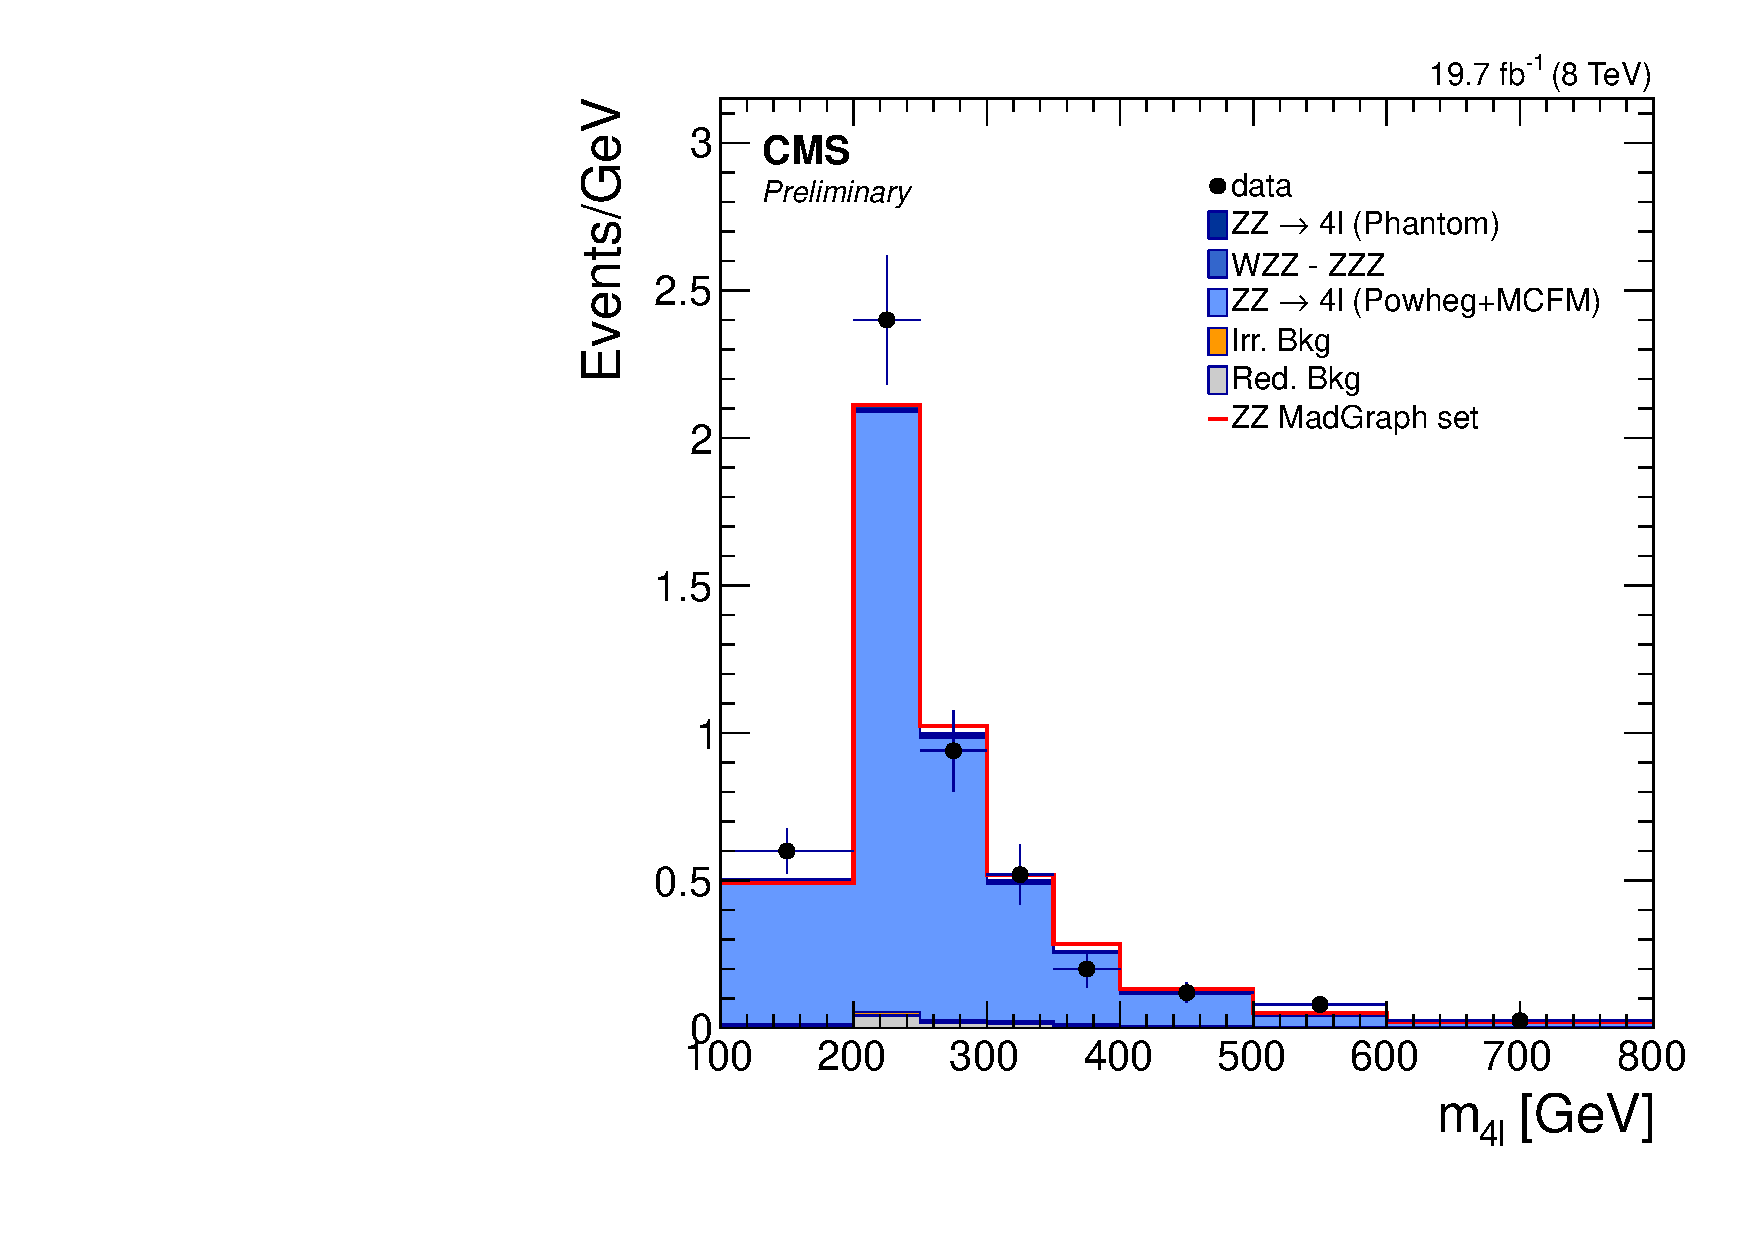
\includegraphics[width=\cmsFigWidth]{Figures/Mass_pow} 
    \caption{Different contributions to the distribution of the reconstructed four-lepton mass. Points represent the data, the stacked filled histogram represents the predictions for $ZZ$ signal and background contributions using \texttt{Powheg} samples to describe $q\bar{q}(qg)\to ZZ\to 4\ell$ processes (while for the stacked histogram outlined in red the \texttt{MadGraph} simulation is used).}
    \label{fig:sig_recoMass}
  \end{center}
\end{figure}
 
\begin{figure}[hbtp]
  \begin{center}
    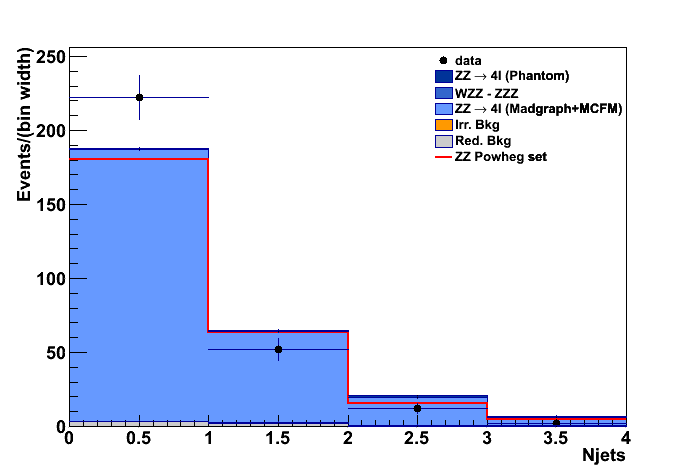
\includegraphics[width=\cmsFigWidth]{Figures/Jets_mad}
    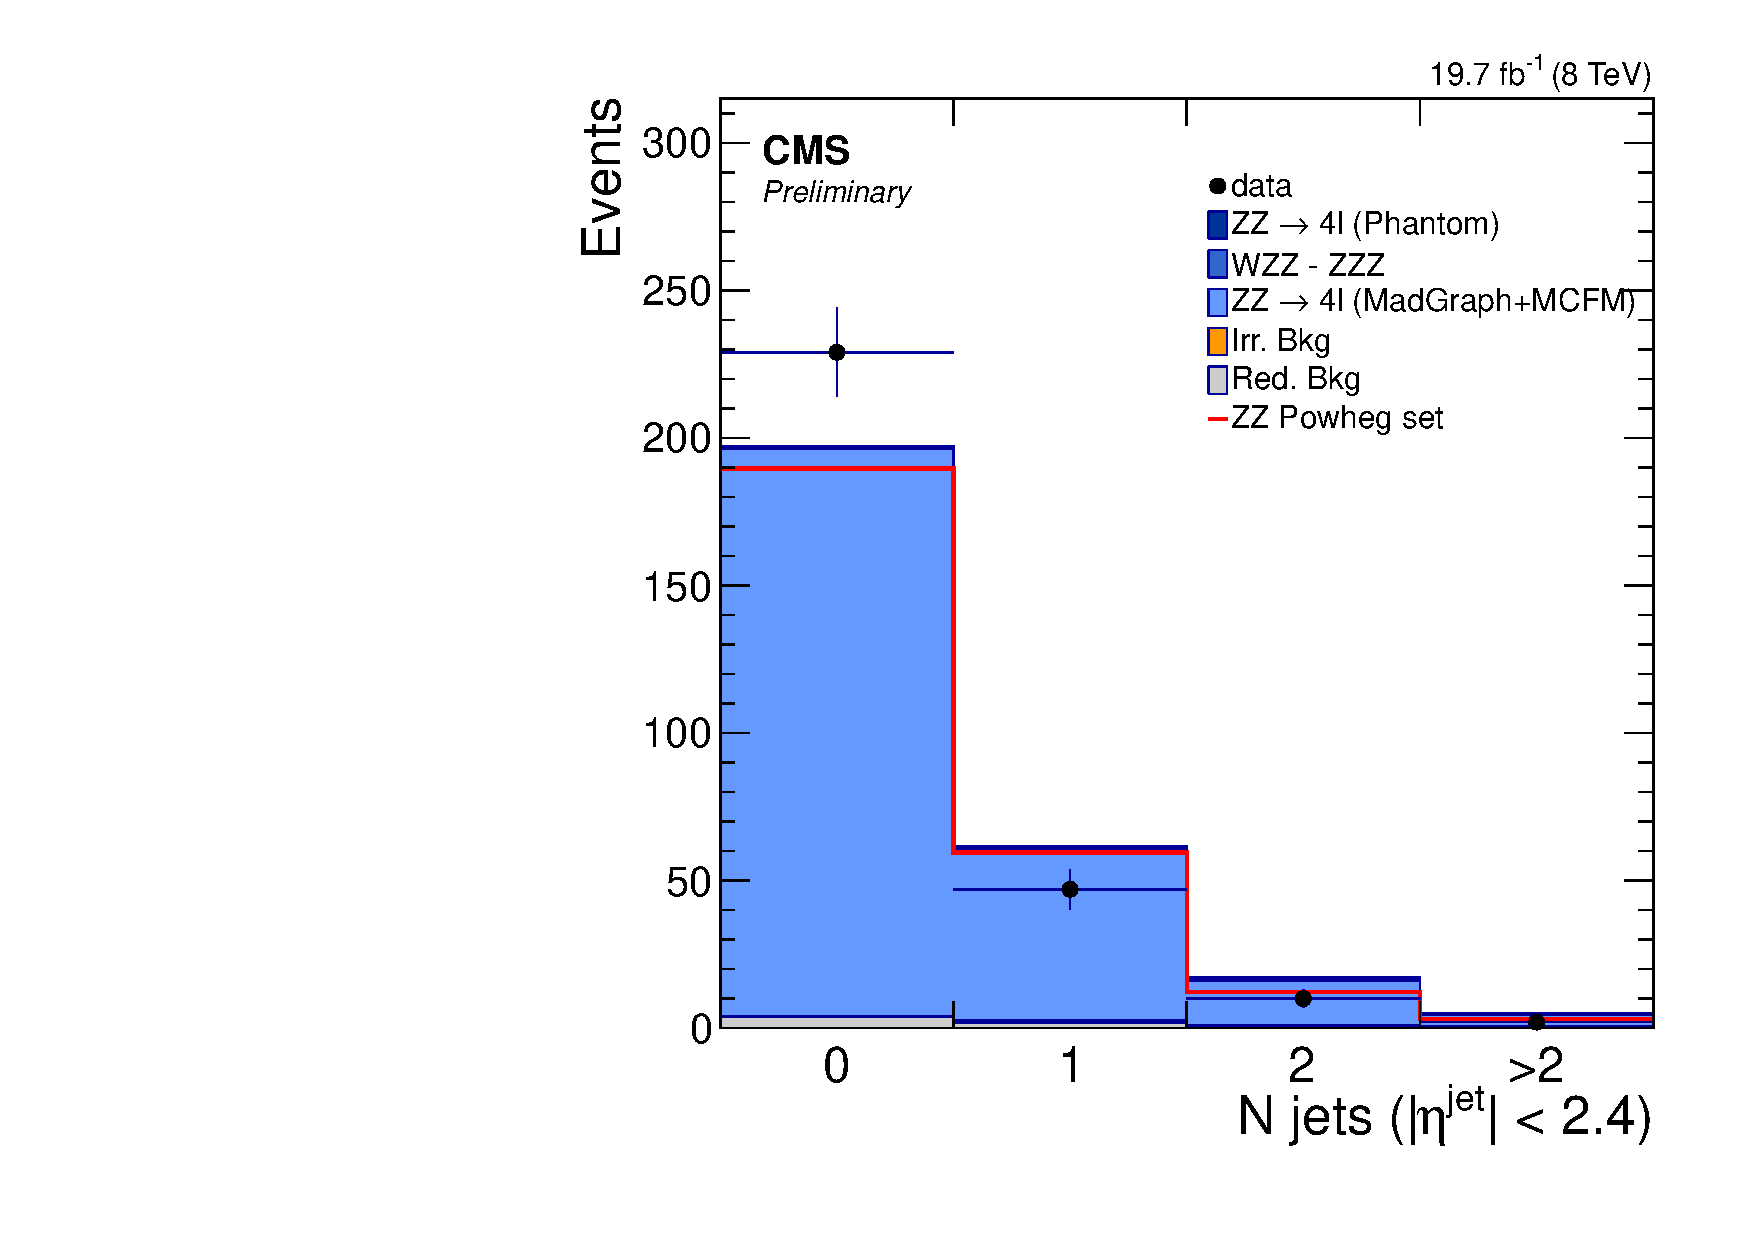
\includegraphics[width=\cmsFigWidth]{Figures/CentralJets_mad}
    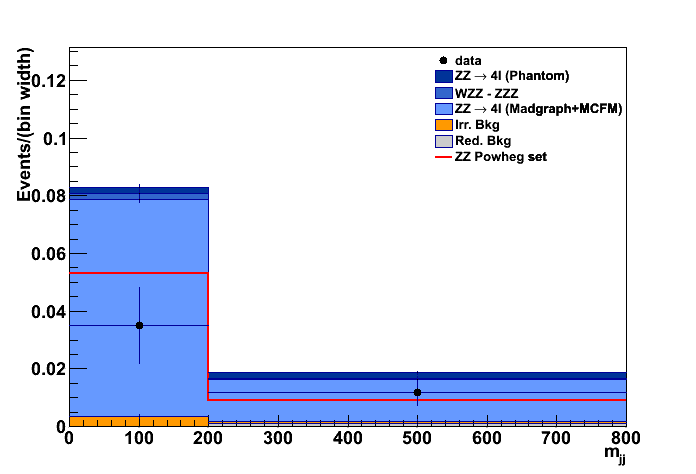
\includegraphics[width=\cmsFigWidth]{Figures/Mjj_mad}
    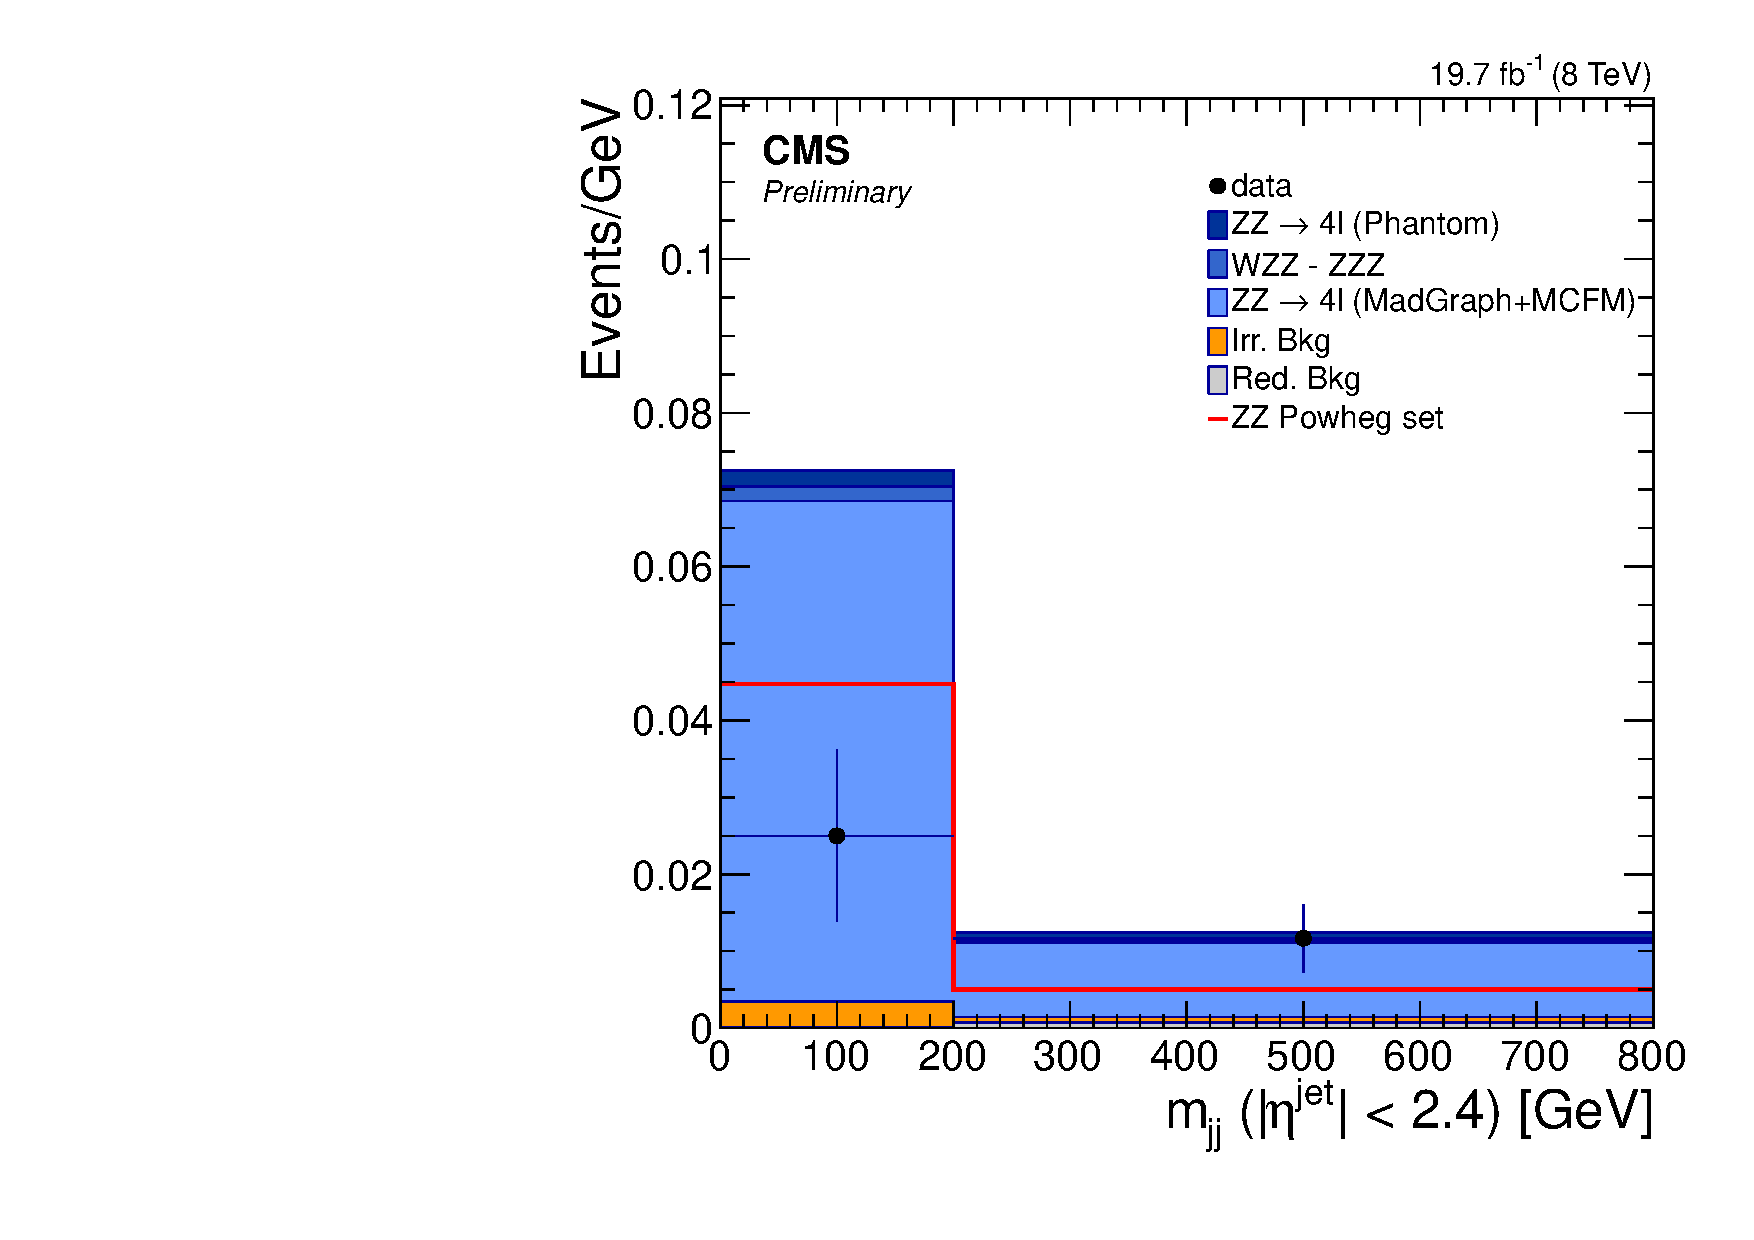
\includegraphics[width=\cmsFigWidth]{Figures/CentralMjj_mad} 
    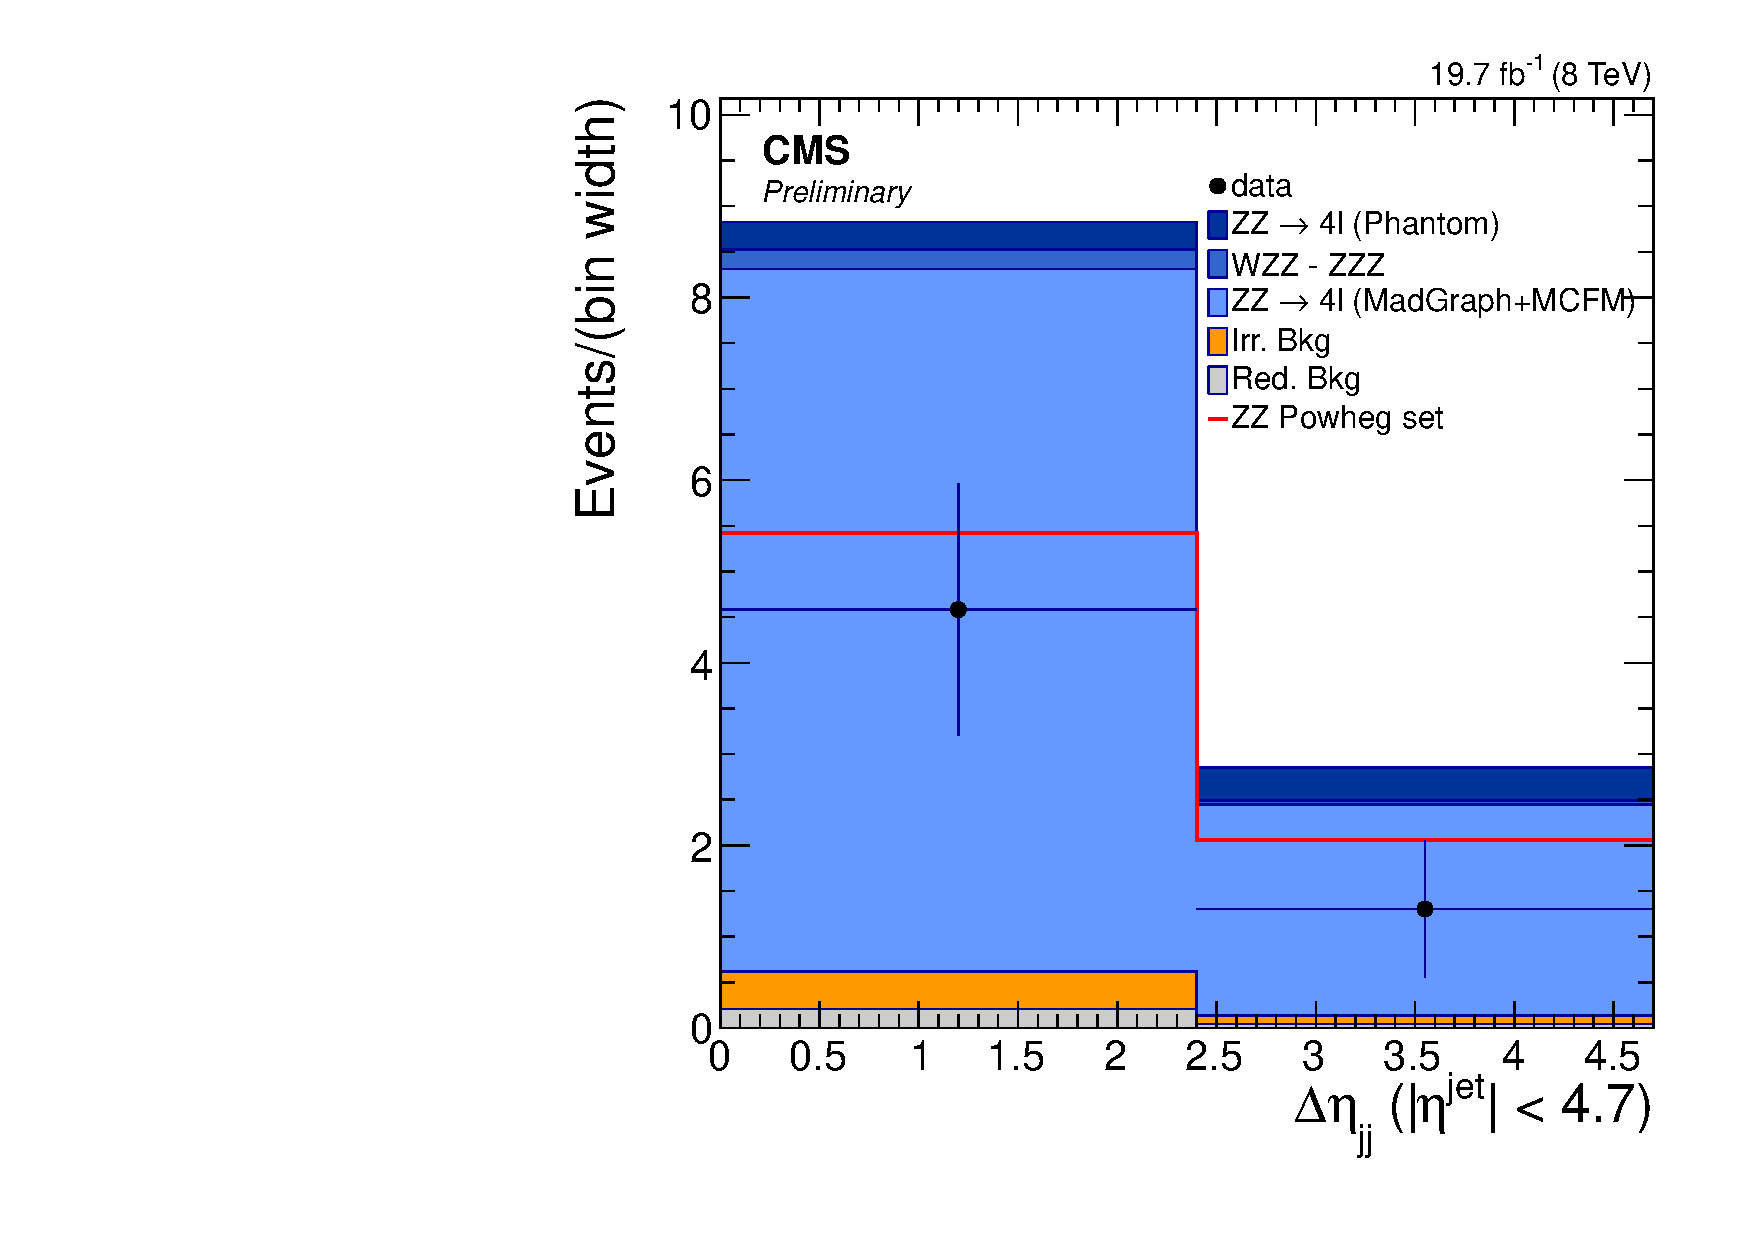
\includegraphics[width=\cmsFigWidth]{Figures/Deta_mad}  
    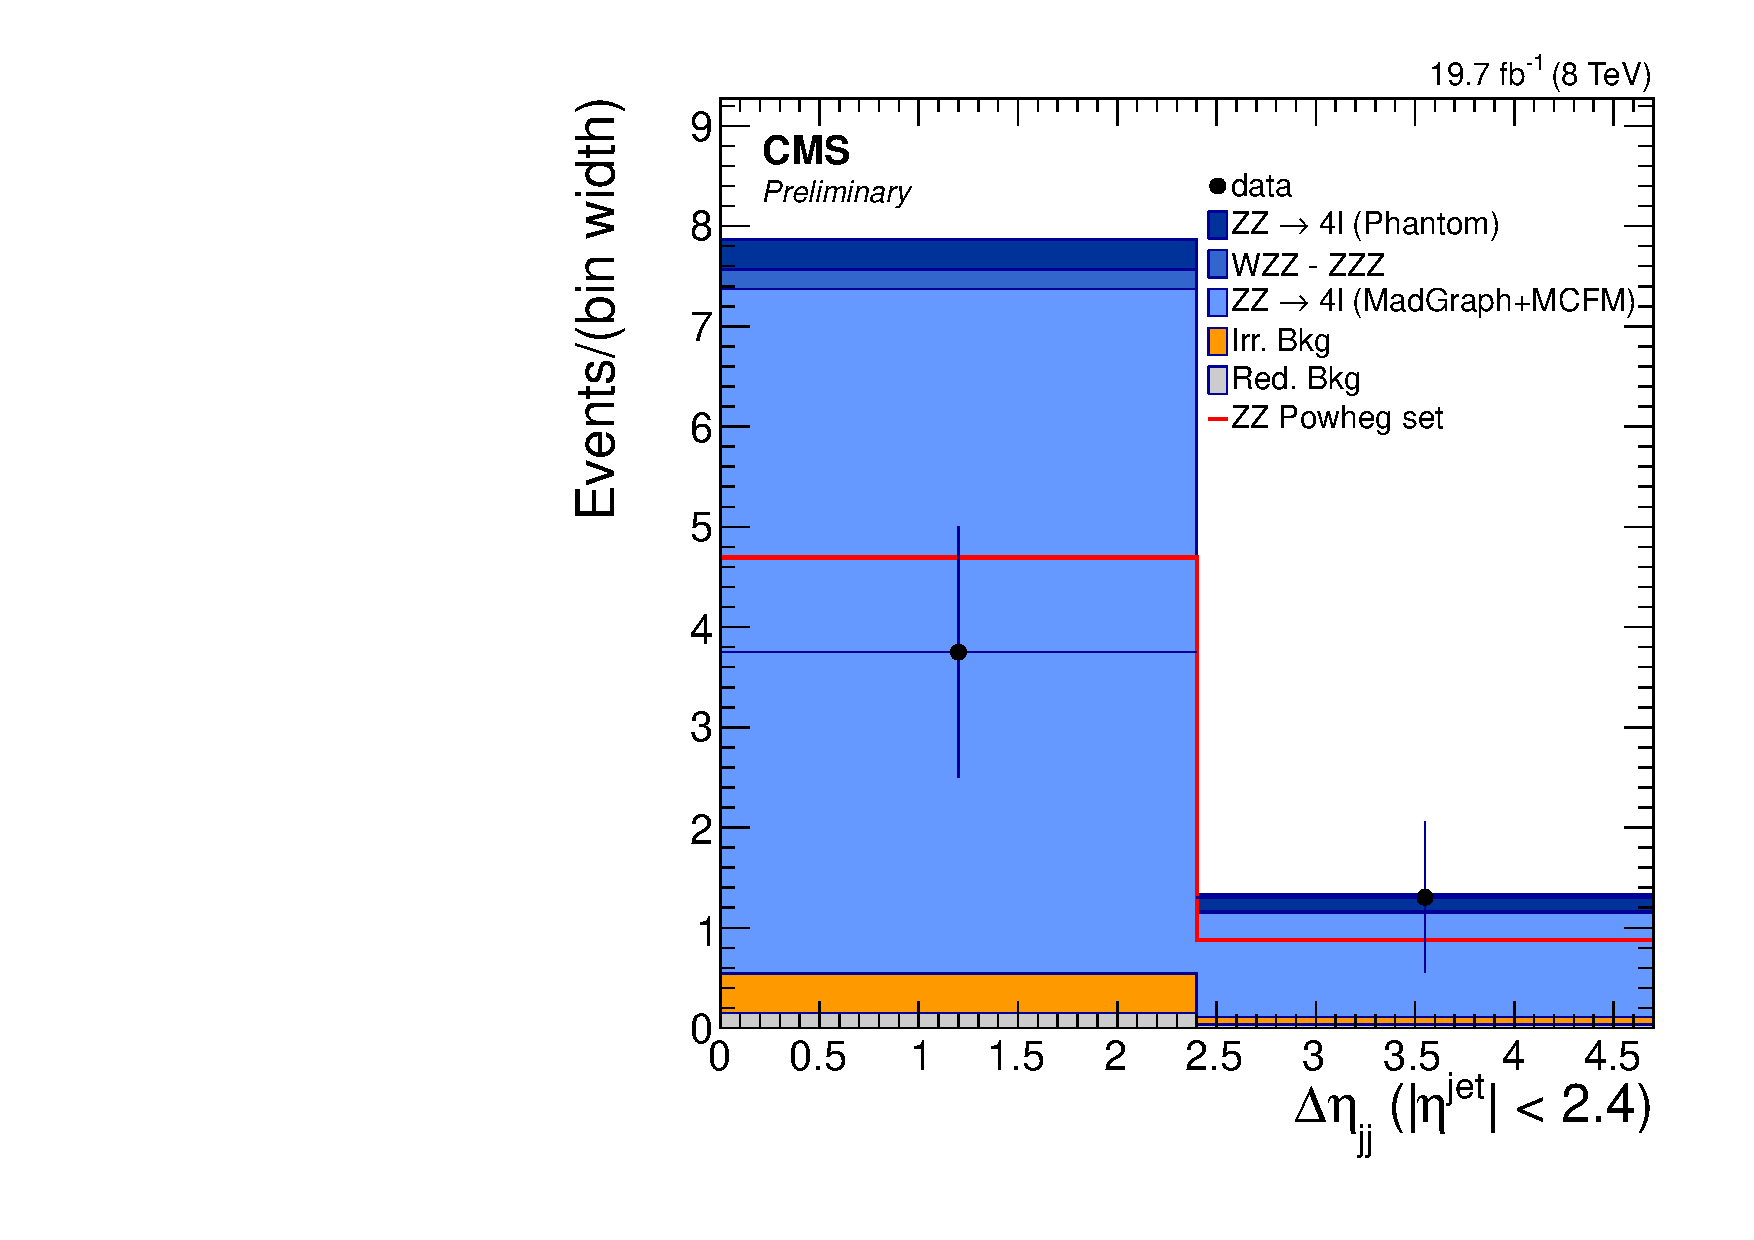
\includegraphics[width=\cmsFigWidth]{Figures/CentralDeta_mad}  
    \caption{Different contributions to the distribution of the reconstructed number of jets produced in the event (top), the invariant mass of the two most energetic jets (center) and the pseudorapidity interval between them (bottom), with $\eta^{jet} < 4.7$ on the left and $\eta^{jet} < 2.4$ on the right. Points represent the data, the stacked filled histogram represents the predictions for $ZZ$ signal and background contributions using \texttt{MadGraph} samples to describe $q\bar{q}(qg)\to ZZ\to 4\ell$ processes (while for the stacked histogram outlined in red the \texttt{Powheg} simulation is used).}
    \label{fig:sig_recoJJ}
  \end{center}
\end{figure}

\begin{figure}[hbtp]
  \begin{center} 
    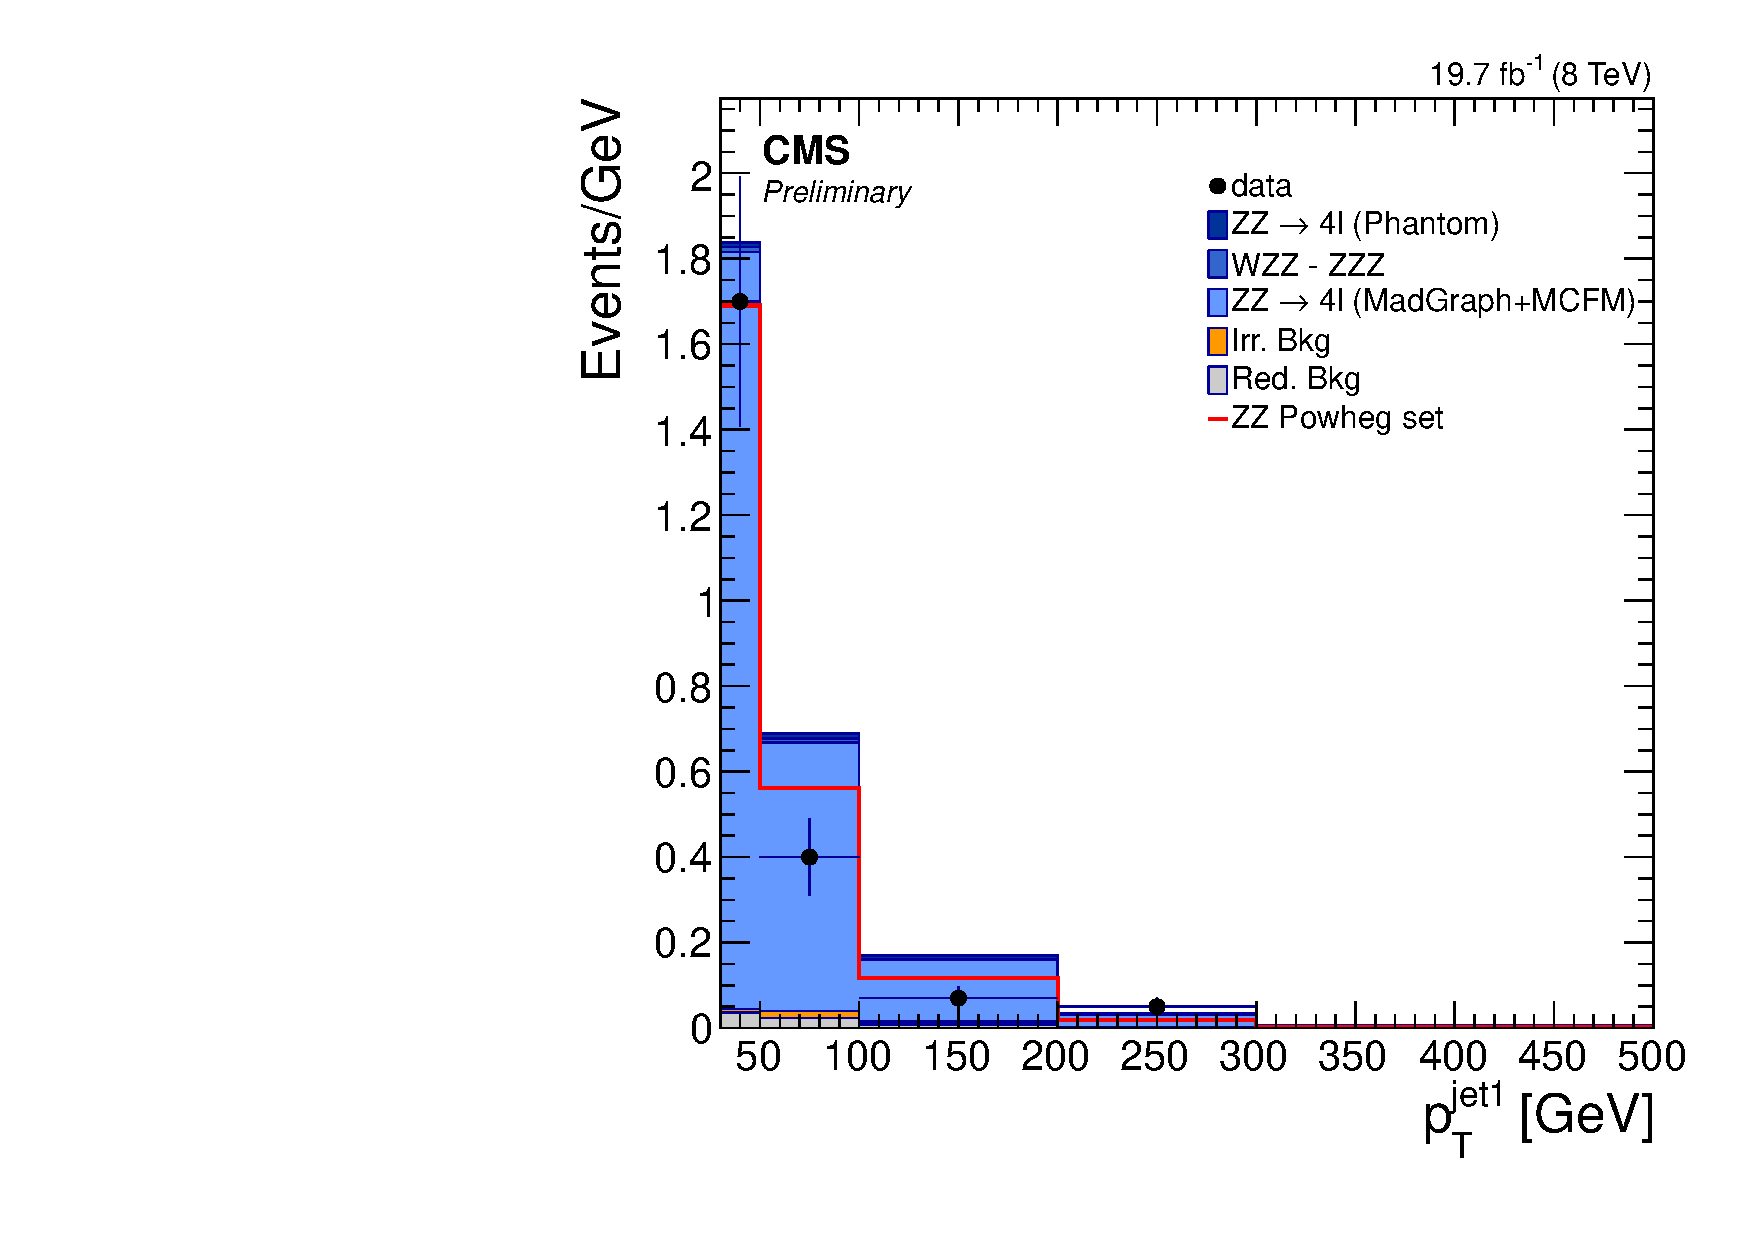
\includegraphics[width=\cmsFigWidth]{Figures/PtJet1_mad}
    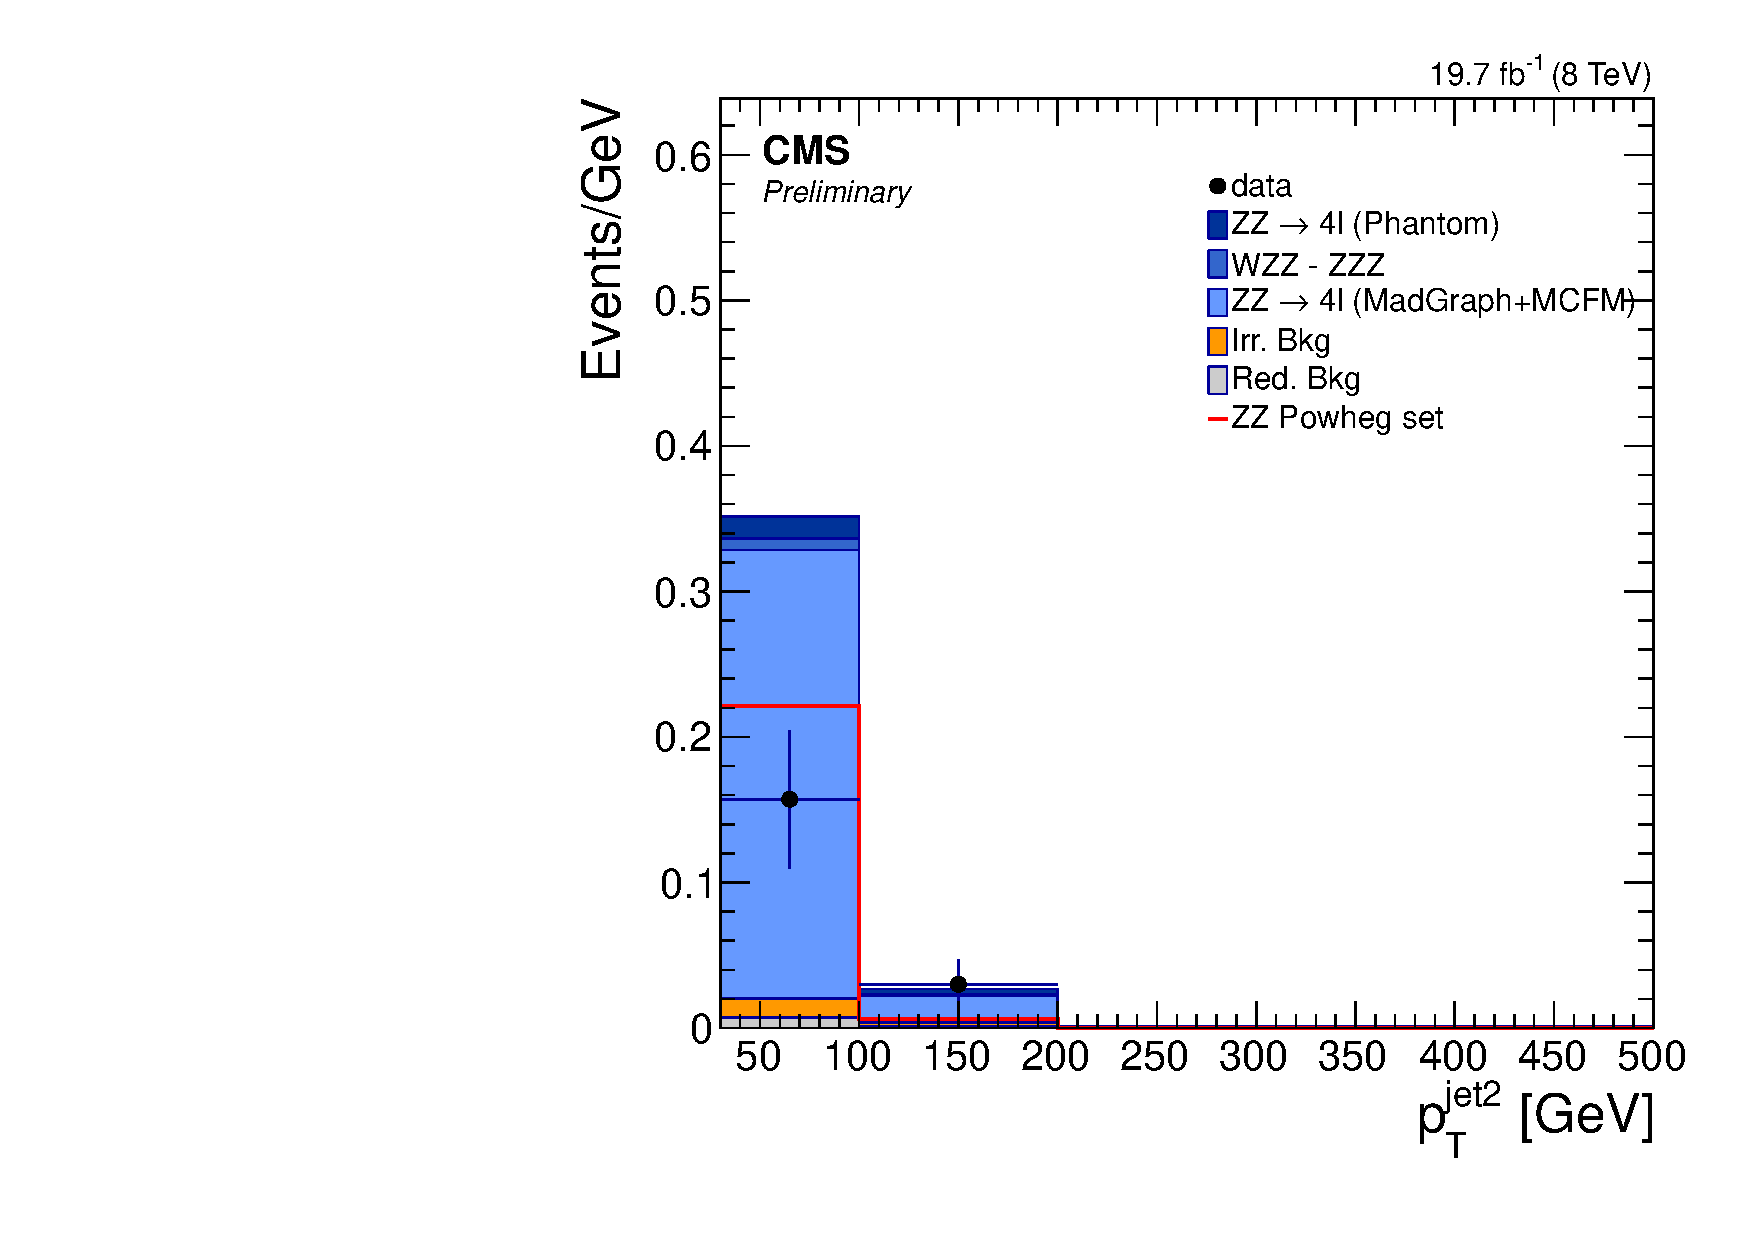
\includegraphics[width=\cmsFigWidth]{Figures/PtJet2_mad} 
    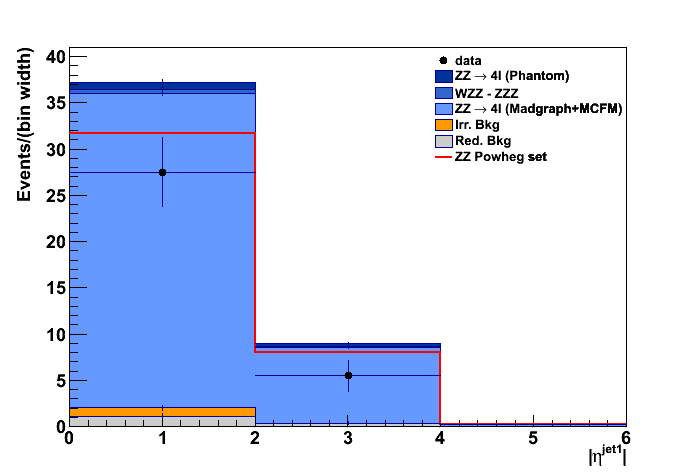
\includegraphics[width=\cmsFigWidth]{Figures/EtaJet1_mad}
    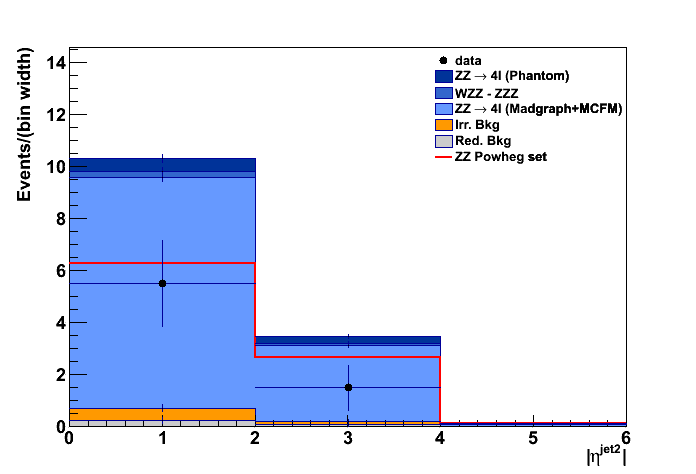
\includegraphics[width=\cmsFigWidth]{Figures/EtaJet2_mad}
    \caption{Different contributions to the distribution of the reconstructed transverse momentum (top) and pseudorapidity (bottom) of the leading (left) and  sub-leading jet (right). Points represent the data, the stacked filled histogram represents the predictions for $ZZ$ signal and background contributions using \texttt{MadGraph} samples to describe $q\bar{q}(qg)\to ZZ\to 4\ell$ processes (while for the stacked histogram outlined in red the \texttt{Powheg} simulation is used).}
    \label{fig:sig_recoPt}
  \end{center}
\end{figure}


\begin{figure}[hbtp]
  \begin{center}
   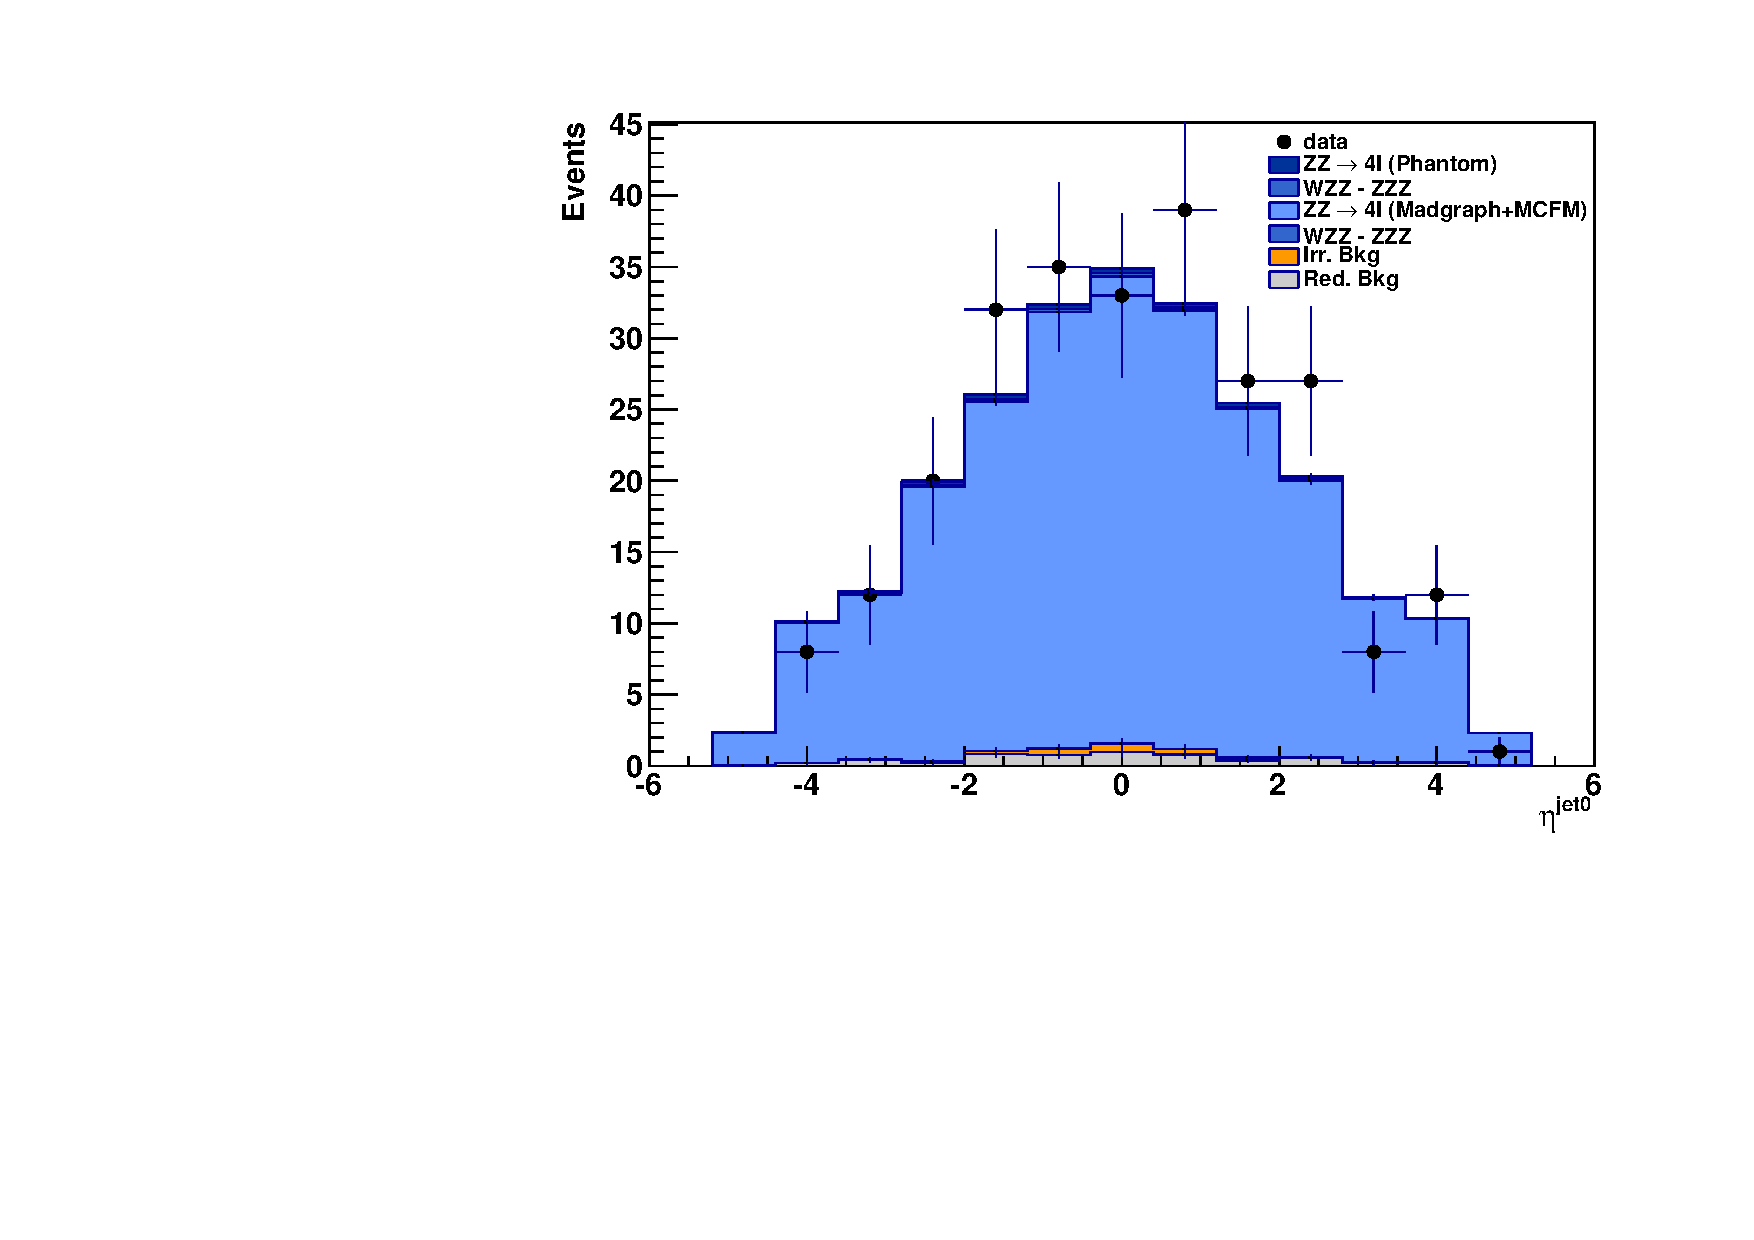
\includegraphics[width=0.8\cmsFigWidth]{Figures/Eta0_mad}    
   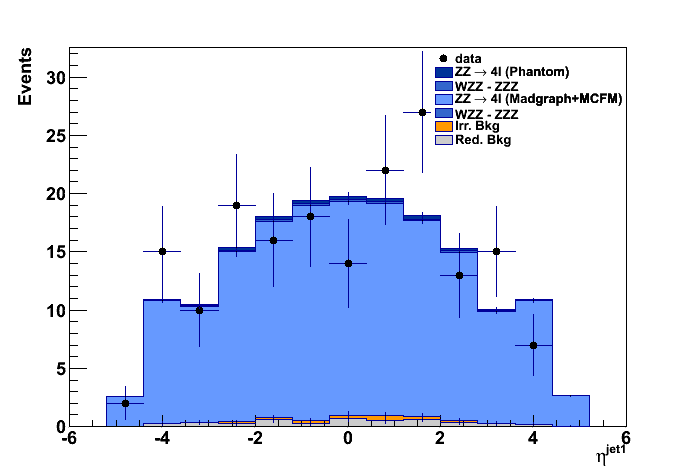
\includegraphics[width=0.8\cmsFigWidth]{Figures/Eta1_mad}
   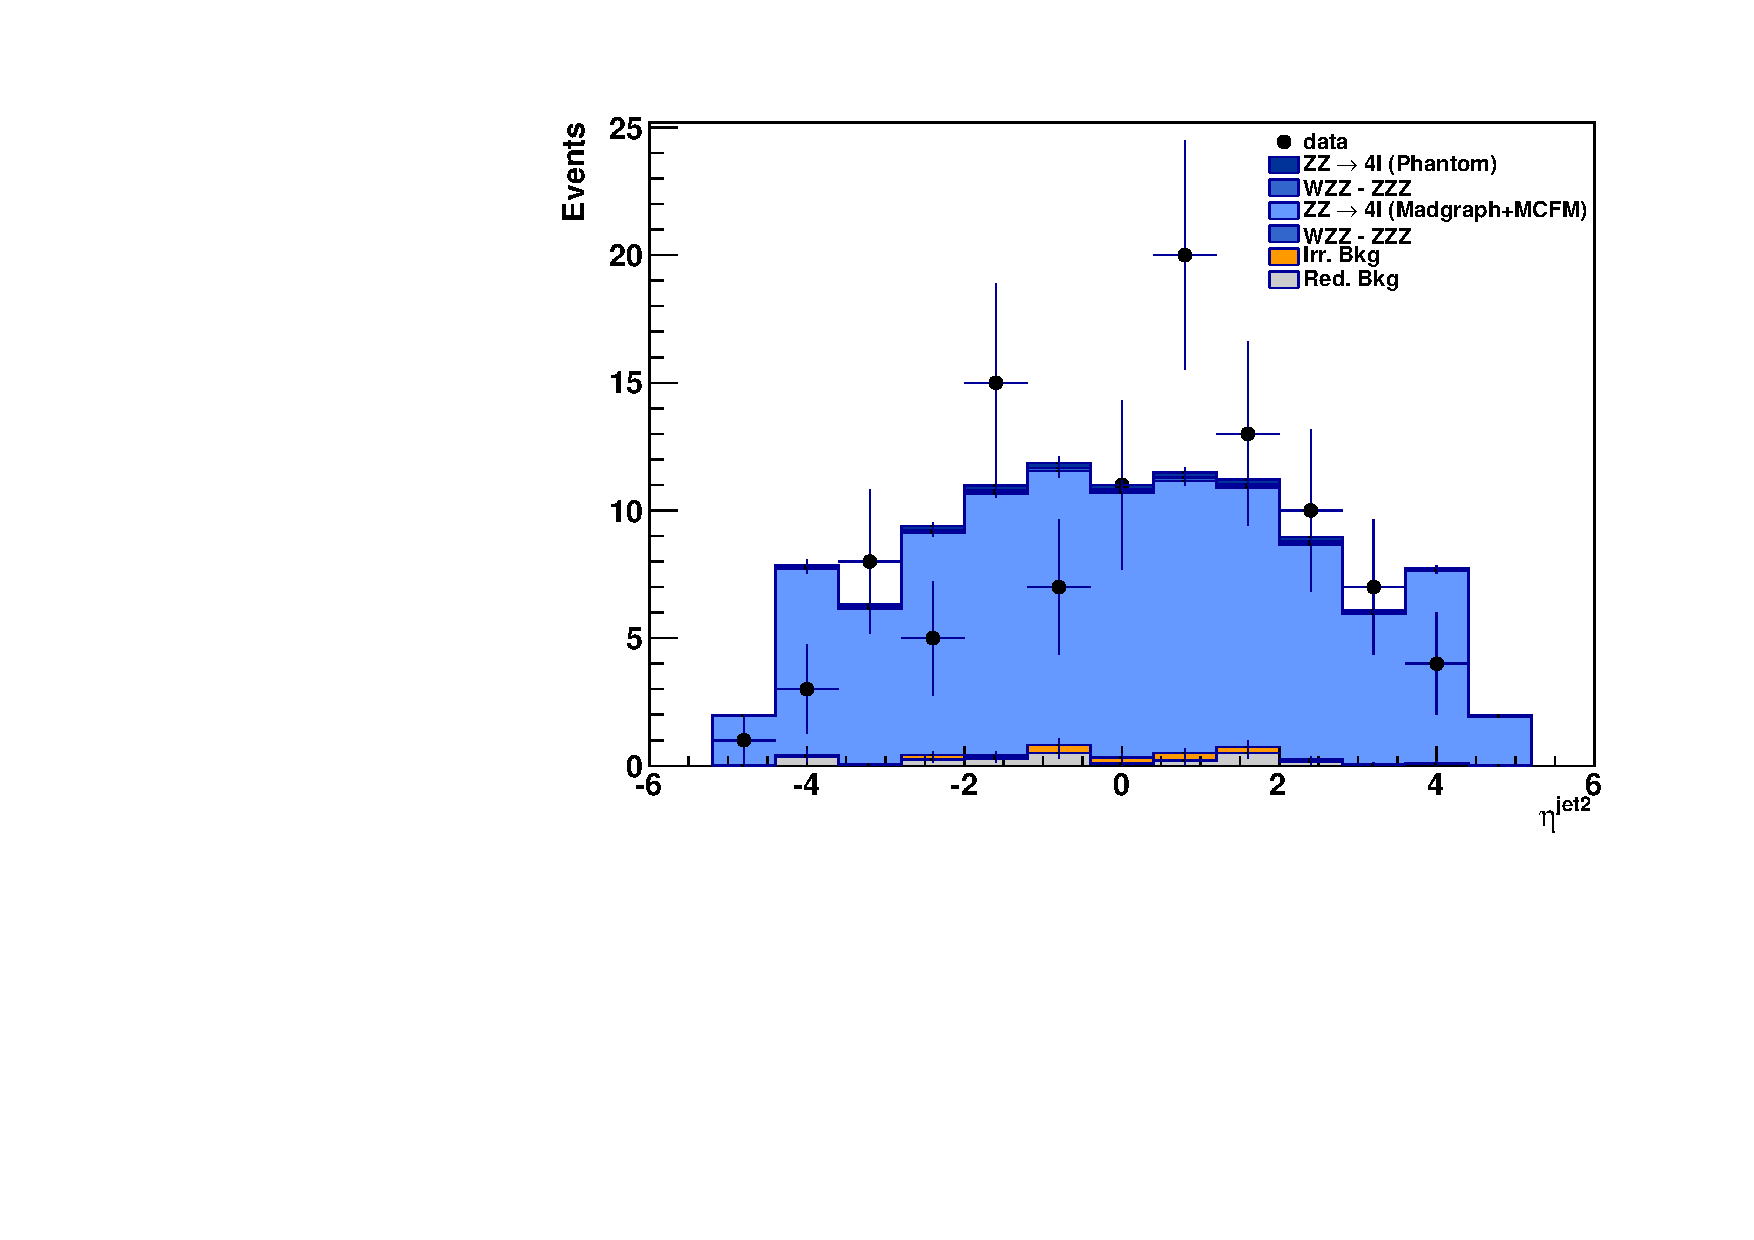
\includegraphics[width=0.8\cmsFigWidth]{Figures/Eta2_mad}
   \caption{Different contributions to the $\eta$-distribution of the most energetic (\cmsLeft), second most energetic (center) and third most energetic (\cmsRight) jet in the event, considering $p_T^{jet}> 10~\mathrm{GeV}$}
   \label{fig:eta_jets}
  \end{center}
\end{figure}
\begin{figure}[hbtp]
  \begin{center}
   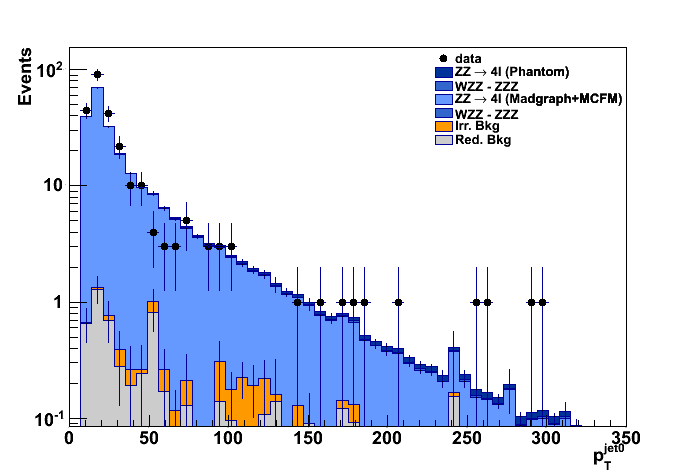
\includegraphics[width=0.8\cmsFigWidth]{Figures/Pt0_mad_log}    
   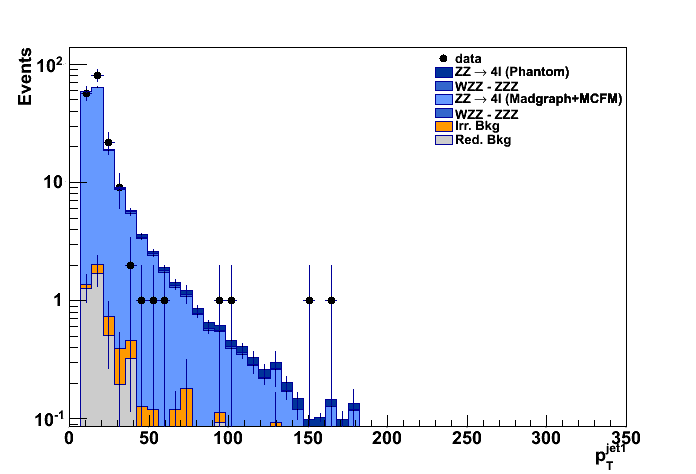
\includegraphics[width=0.8\cmsFigWidth]{Figures/Pt1_mad_log}
   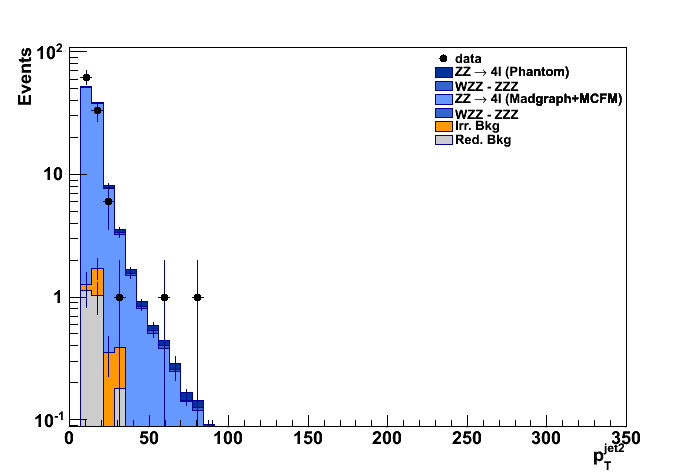
\includegraphics[width=0.8\cmsFigWidth]{Figures/Pt2_mad_log}
   \caption{Different contributions to the $p_{T}$-distribution of the most energetic (\cmsLeft), second most energetic (center) and third most energetic (\cmsRight) jet in the event, considering  $p_T^{jet}> 10~\mathrm{GeV}$.}
   \label{fig:pt_jets}
  \end{center}
\end{figure}
Table~\ref{tab:xs} lists the total cross-section obtained from each individual decay channel as well as the
total cross-section based on the combination of all channels. The measured cross-section agrees
with the theoretical value of $7.5\pm 0.5$ pb calculated with \texttt{MCFM 6.6}. In this calculation, the
contribution from $q\bar{q} \to ZZ$ is obtained at NLO, while the smaller contribution (approximately
6\%) from $ gg \to ZZ$ is obtained at LO.

\begin{table*}[htbH]
\begin{center}
\topcaption{The signal yield is obtained by subtracting from the observed yield the expected background events. Statistical uncertainties are reported.
\label{tab:sig_yields}}
\begin{tabular}{lcccc}
\hline Final state & Observed data& Irreducible background & Reducible background & Final yield\\
\hline $ZZ\to 4\mu $ & $ 80 \pm 8.9 $ & $ 0.52 \pm 0.10 $ & $ 0.92 \pm 0.61 $ & $ 78.6 \pm 8.9$ \\ 
$ZZ\to 4e $ & $56 \pm 7.5 $ & $ 0.21 \pm 0.06 $ & $ 1.93 \pm 0.72 $ & $ 54.0 \pm 7.5 $\\
$ZZ\to 2e2\mu$ & $ 152 \pm 12 $ & $ 1.16 \pm 0.15 $ & $ 3.3 \pm 1.1 $ & $ 148 \pm 12 $\\
\hline
\textbf{$ZZ\to 4\ell$} & $ 288 \pm 17 $ & $1.89 \pm 0.19 $ & $ 6.2 \pm 1.4 $ & $ 281 \pm17 $ \\ 
\hline 
\end{tabular}
\end{center}
\end{table*}

%\begin{table*}[htbH]
%\begin{center}
%\topcaption{The total $ZZ$ production cross-section as measured in each decay channel and for the
%combination of all channels.
%\label{tab:xs}}
%\begin{tabular}{lc}
%\hline Final state & Total cross-section [pb]\\
%\hline $ZZ\to 4\mu $ & $7.5\pm 0.9$ (stat.) $\pm 0.3$ (syst.)\\
%$ZZ\to 4e $ &  $7.4\pm 1.0$ (stat.) $\pm 0.3$ (syst.)\\
%$ZZ\to 2e2\mu$ & $8.3\pm 0.7$ (stat.) $\pm 0.4$ (syst.)\\
%\hline
%\textbf{$ZZ\to 4\ell$} &  $7.6\pm 0.5$ (stat.) $\pm 0.3$ (syst.)\\
%\hline \\
%\end{tabular}
%\end{center}
%\end{table*}
\begin{table*}[htbH]
\begin{center}
\caption{The total $ZZ$ production cross-section as measured in each decay channel and for the
combination of all channels in the fiducial region $60< m_{Z_{1}}, m_{Z_{}} < 120~\mathrm{GeV}$.}
\label{tab:xs}
%\scalebox{1.5\columnwidth}{!}{
%\doublespacing{
\begin{tabular}{lc}
\hline Process & Total cross-section [pb]\\
\hline $pp\to ZZ(4\mu) $ & $7.46\pm 0.86~\mathrm{(stat.)}^{+0.45}_{- 0.47}~\mathrm{(syst.)}$\\
$pp\to ZZ(4e) $ &  $7.32\pm 1.02~\mathrm{(stat.)}^{+0.59}_{- 0.62}~\mathrm{(syst.)}$\\
$pp\to ZZ(2e2\mu)$ & $8.22\pm 0.70~\mathrm{(stat.)}^{+0.59}_{- 0.61}~\mathrm{(syst.)}$\\
\hline
\textbf{$pp\to ZZ(4\ell)$} & $7.76 \pm 0.48~\mathrm{(stat.)}^{+0.47}_{- 0.47}~\mathrm{(syst.)}$ \\
\hline \\
\end{tabular}%}
\end{center}
\end{table*}
The fiducial region in which the cross-section is extracted, defined requiring two $Z$ bosons with mass between 60 and 120 GeV, is much wider with respect to the region in which events are really measured, limited by the active volume of the detector, as shown by the low values of $A\cdot \epsilon$. In order to obtain a measurement closer to what is effectively reconstructed by the detector, a \emph{tight fiducial region} is defined as follows:
\begin{itemize}
\item $60 < m_{Z_1},m_{Z_2} < 120~\mathrm{GeV}$;
%\item $m_{4\ell} > 100~\mathrm{GeV}$;
\item at least one lepton with $p_T > 20~\mathrm{GeV}$ and another one with $p_T > 10~\mathrm{GeV}$;
\item electrons must have $p_T^e > 7~\mathrm{GeV}$ and $|\eta^e|<2.5$;
\item muons must have $p_T^{\mu} > 5~\mathrm{GeV}$ and $|\eta^{\mu}|<2.4.$
\end{itemize}
The last three requirements correspond to the $\eta$ and $p_T$-acceptance of the detector and are the same selection criteria demanded when leptons are built, while the first requirement corresponds to the definition of the wider region applied for the previous inclusive measurement. The formula used in this case is
$$\sigma_{ZZ} = \frac{N_{data}-N_{bkg}}{\mathcal{L}\cdot A \cdot \epsilon},$$
where the branching-ratio factor is removed in order to obtain the cross-section of the $pp\to ZZ\to 4\ell$ process, and the new values of $ A \cdot \epsilon$ are reported in Table~\ref{tab:Aeps_tight}. The cross-section measurements obtained in this tight region are listed in Table~\ref{tab:tightxs}.
\begin{table*}[htbH]
\begin{center}
\topcaption{$A\cdot \epsilon$ for the three final states used in the $pp\to ZZ \to 4\ell$ cross-section measurement in the tight fiducial region.
The values reported are a product of the detector geometrical acceptance and
the object reconstruction and event identification efficiency. \label{tab:Aeps_tight}}
\begin{tabular}{cc}
\hline Final State & $A\cdot\epsilon$\\
\hline $4\mu$ & 84 \%  \\
$4e$ & 55\%\\
$2e2\mu$ & 69\%\\
\hline
\end{tabular}
\end{center}
\end{table*}
\begin{table*}[htbH]
\begin{center}
\topcaption{The total $ZZ$ production cross-section as measured in each decay channel and for the
combination of all channels in the tight fiducial region.
\label{tab:tightxs}}
\begin{tabular}{lc}
\hline Final state & Total cross-section [fb]\\
\hline $ZZ\to 4\mu $ & $4.74\pm 0.54$ (stat.) $^{+0.17}_{-0.18}$ (syst.)\\
$ZZ\to 4e $ &  $4.99\pm 0.69$ (stat.) $^{+0.32}_{-0.35}$ (syst.)\\
$ZZ\to 2e2\mu$ & $10.77\pm 0.90$ (stat.) $^{+0.55}_{-0.59}$ (syst.)\\
\hline
\textbf{$ZZ\to 4\ell$} &  $20.50\pm 1.26$ (stat.) $^{+0.82}_{-0.85}$ (syst.)\\
\hline \\
\end{tabular}
\end{center}
\end{table*}

\begin{figure}[hbtp]
  \begin{center}
    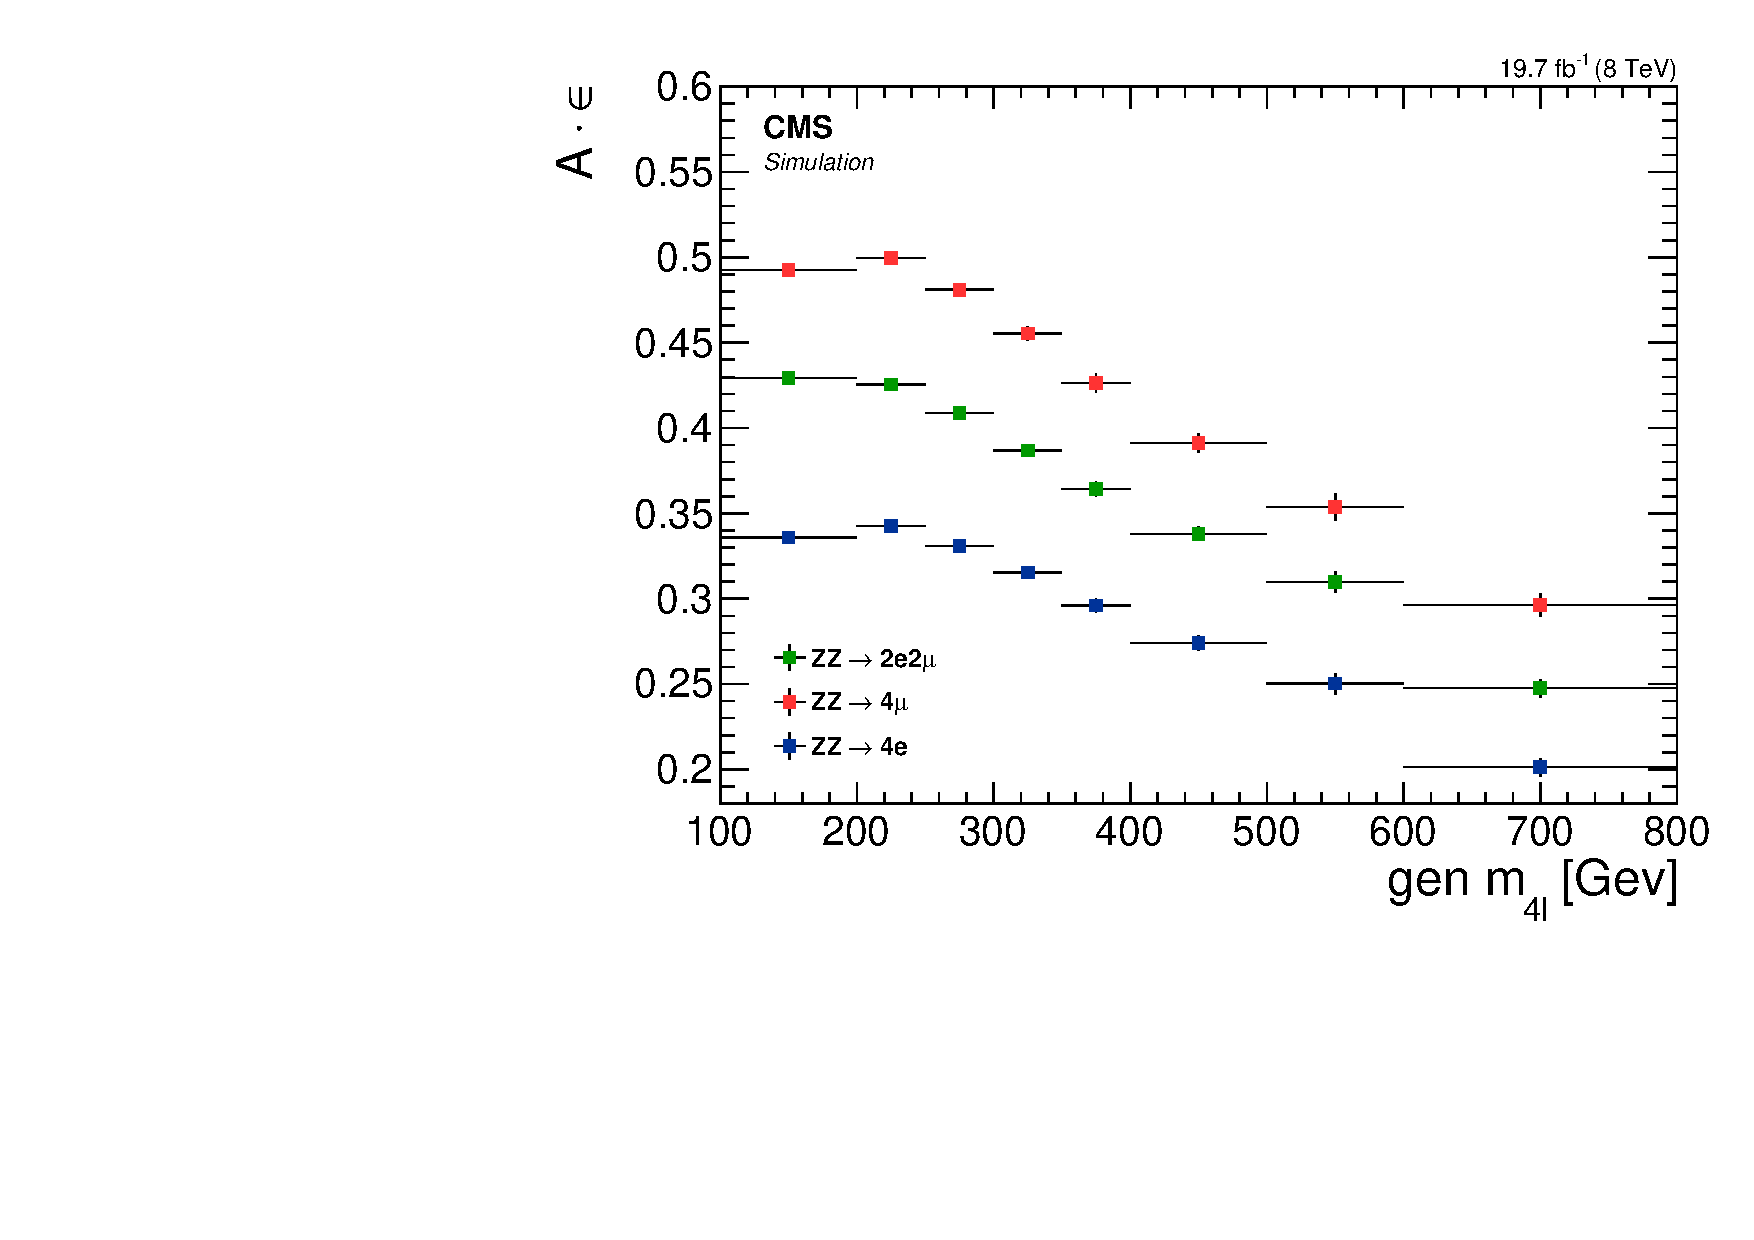
\includegraphics[width=\cmsFigWidth]{Figures/DiffAcceptance_Mass_Pow}
    
\includegraphics[width=\cmsFigWidth]{Figures/DiffAcceptance_Jets_Mad}
    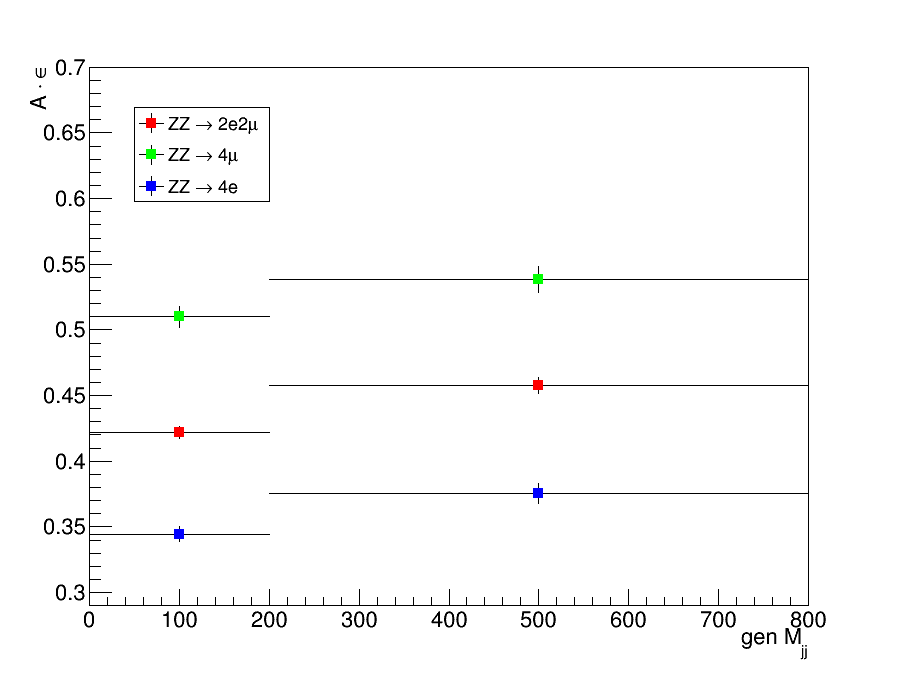
\includegraphics[width=\cmsFigWidth]{Figures/DiffAcceptance_Mjj_Mad}
    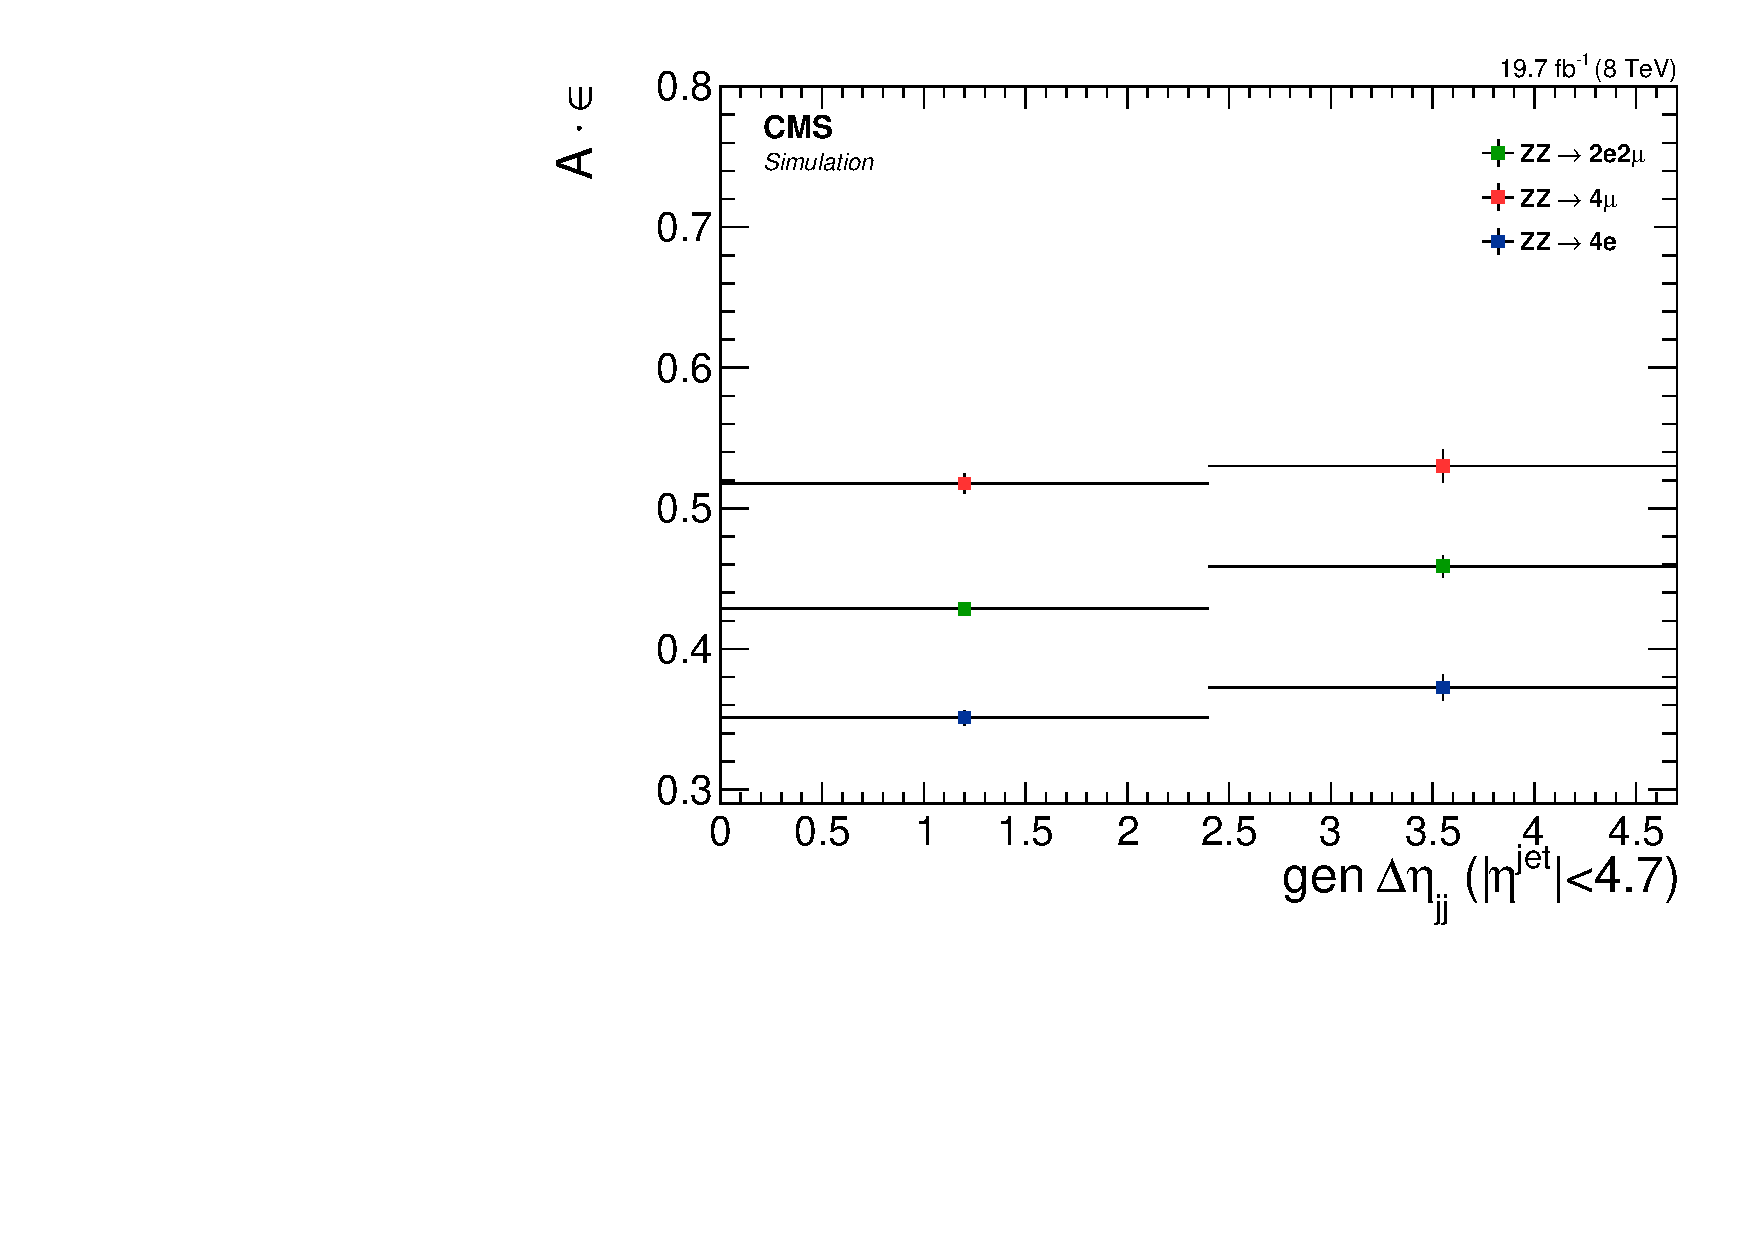
\includegraphics[width=\cmsFigWidth]{Figures/DiffAcceptance_Deta_Mad}
    %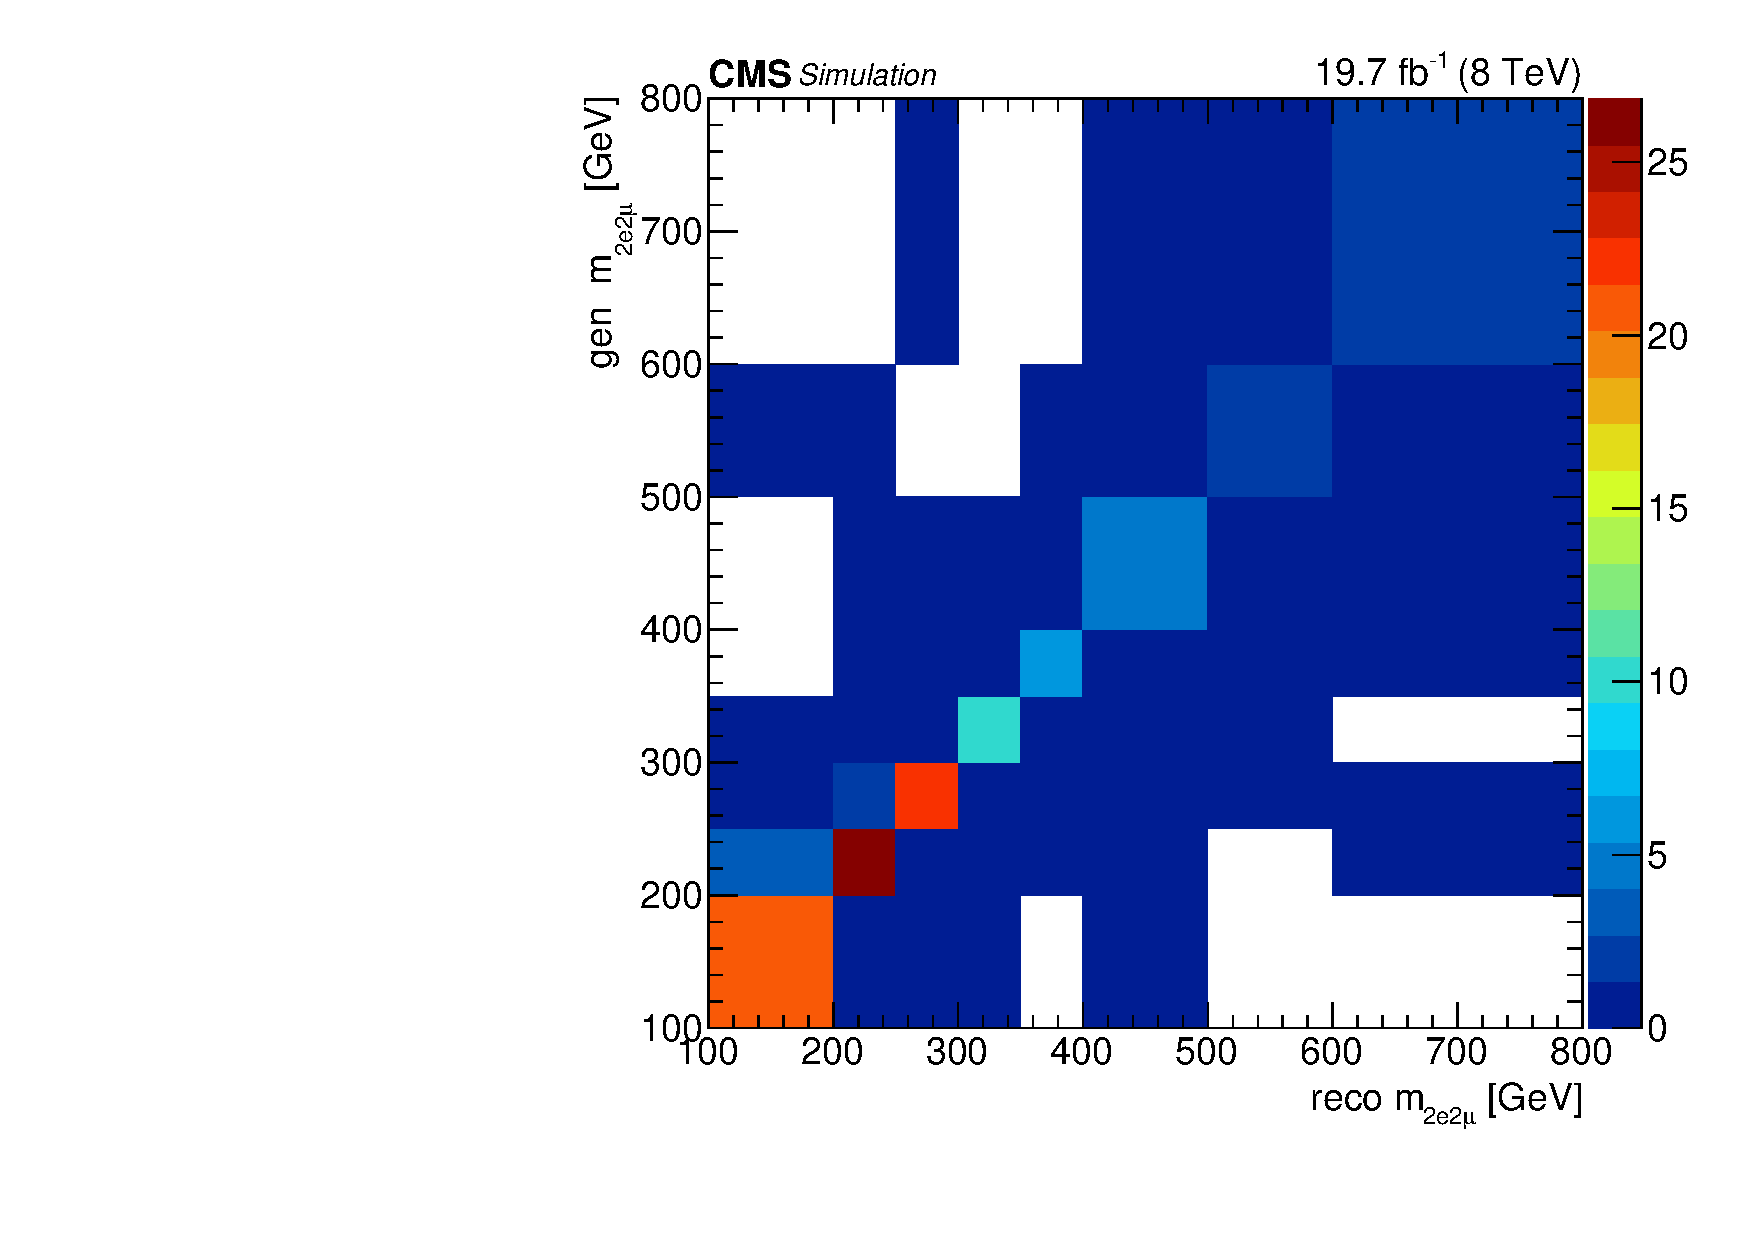
\includegraphics[width=\cmsFigWidth]{Figures/ResMat_qqggJJ_Mass_ZZTo2e2m_st_01_Pow}     
 %   to generate (a) and (b) labels under the figures, you can use subfloat, but this is not recommended: takes too much space
 %   \subfloat[]{
\includegraphics[width=0.2\textwidth]{CMS-bw-logo}}\subfloat[]{
\includegraphics[width=0.2\textwidth]{CMScol}}
    \caption{Acceptance ($A \cdot \epsilon$) computed in the wider fiducial region as a function of $m_{ZZ}$  (top left), $N\ jets$  (top right), $m_{jj}$ (bottom left) and $\Delta\eta_{jj}$
distributions, according to the final state: 
      $4\mu$ (green), $4e$ (blue), $2e2\mu$  (red). Distributions are obtained using the  \texttt{Powheg} set of samples for  $m_{ZZ}$ and 
     the  \texttt{MadGraph} set of samples for the other variables.} 
    \label{fig:A_diff}
  \end{center}
\end{figure}
\begin{figure}[hbtp]
  \begin{center}
    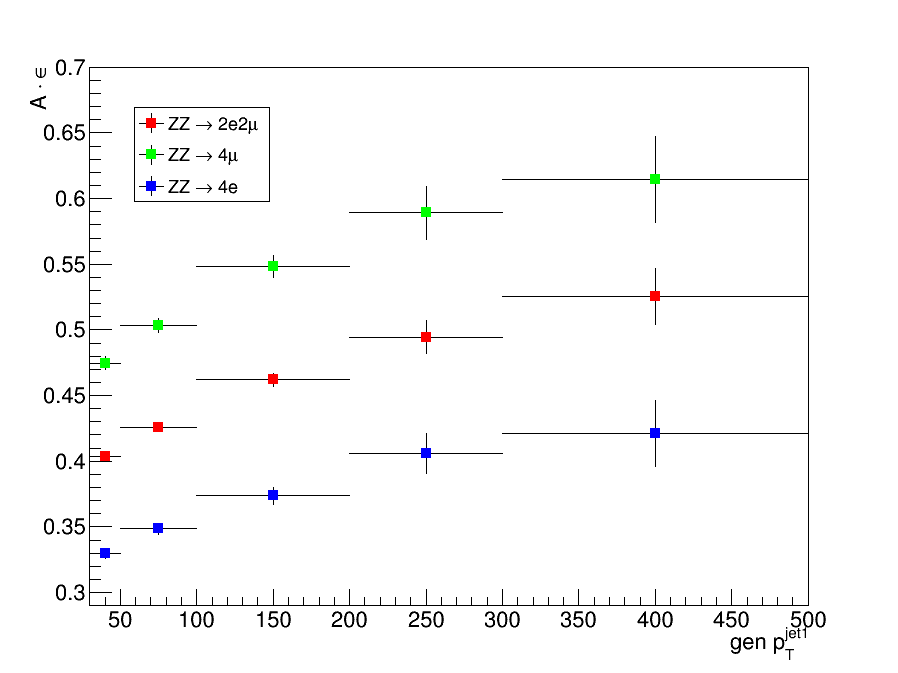
\includegraphics[width=\cmsFigWidth]{Figures/DiffAcceptance_PtJet1_Mad}
    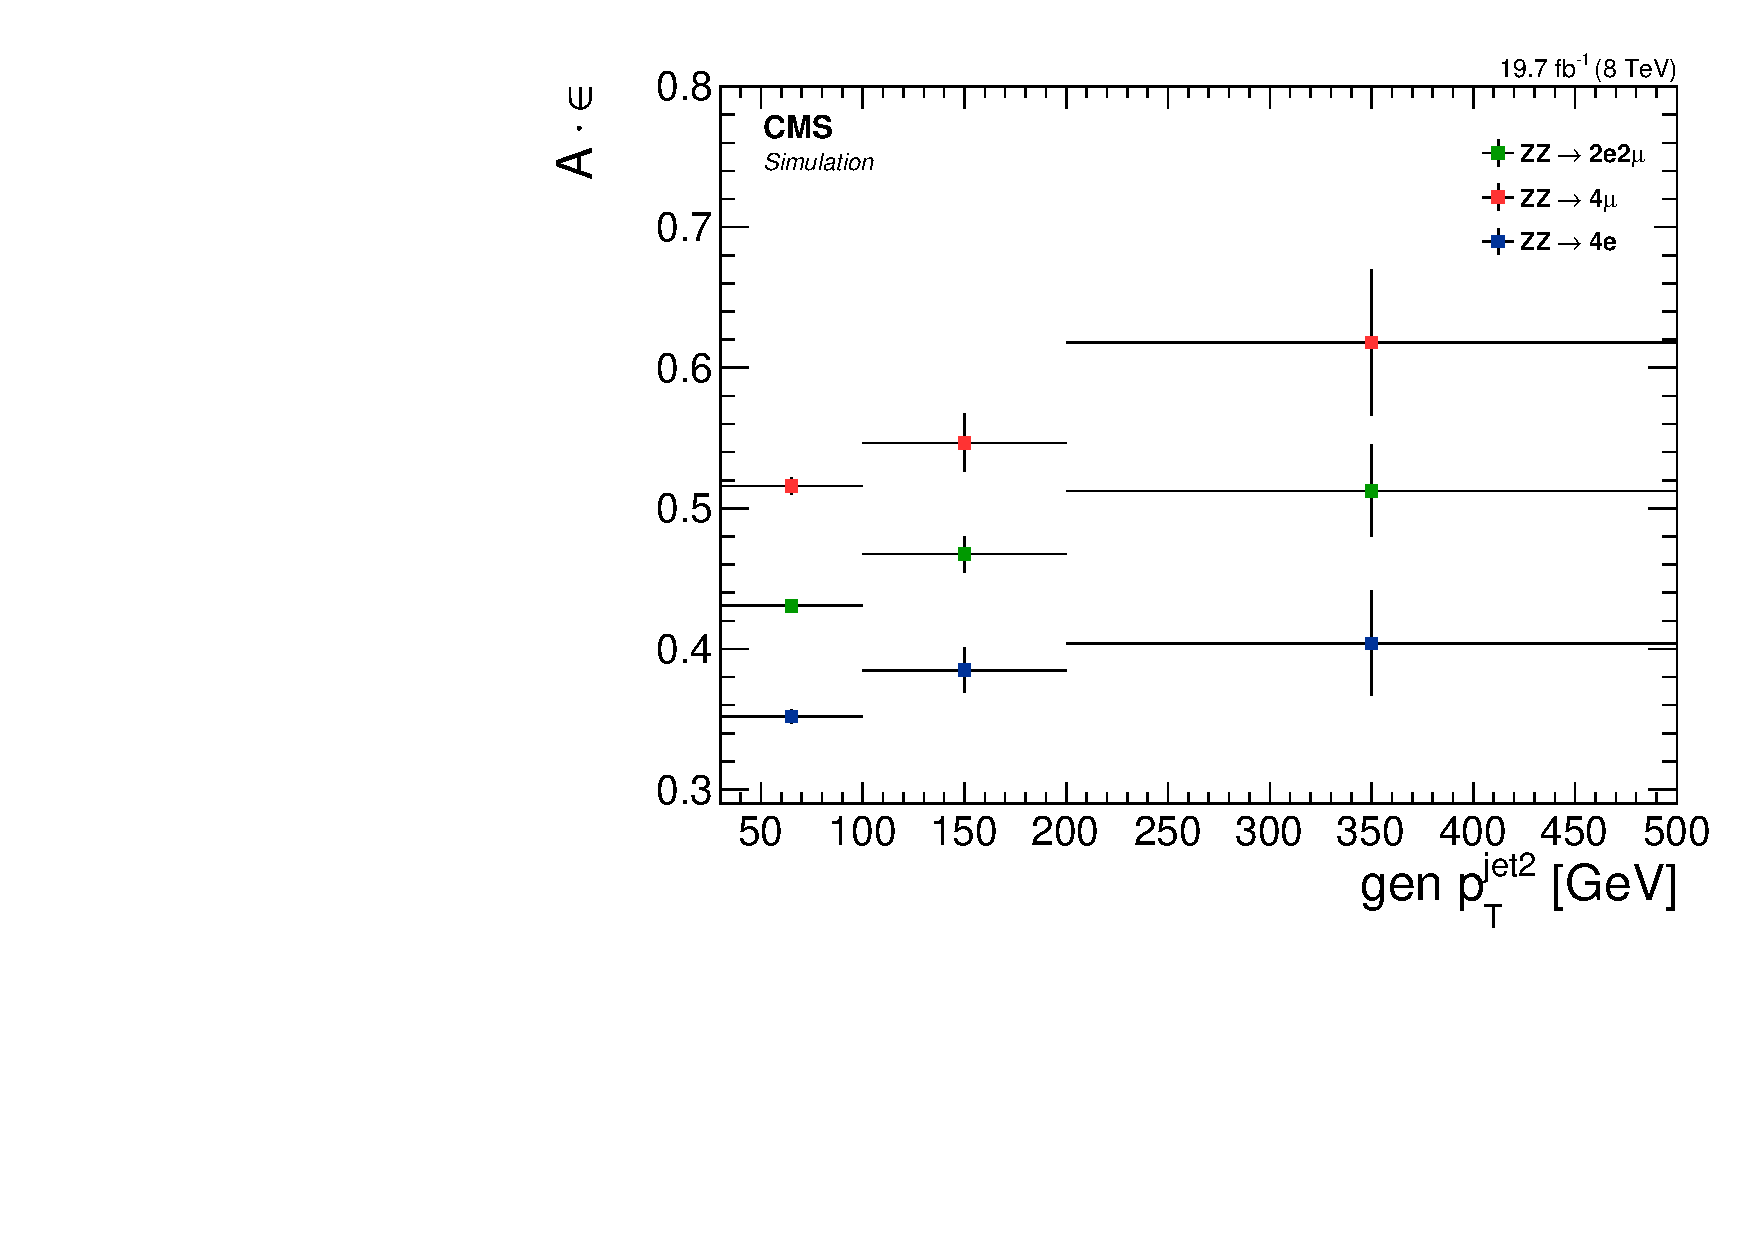
\includegraphics[width=\cmsFigWidth]{Figures/DiffAcceptance_PtJet2_Mad}
    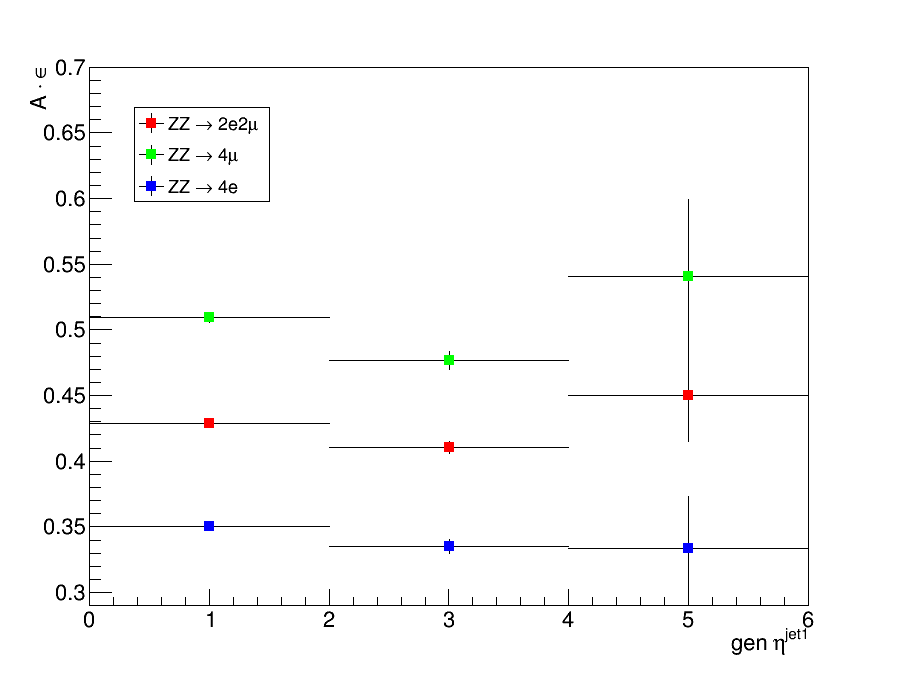
\includegraphics[width=\cmsFigWidth]{Figures/DiffAcceptance_EtaJet1_Mad}
    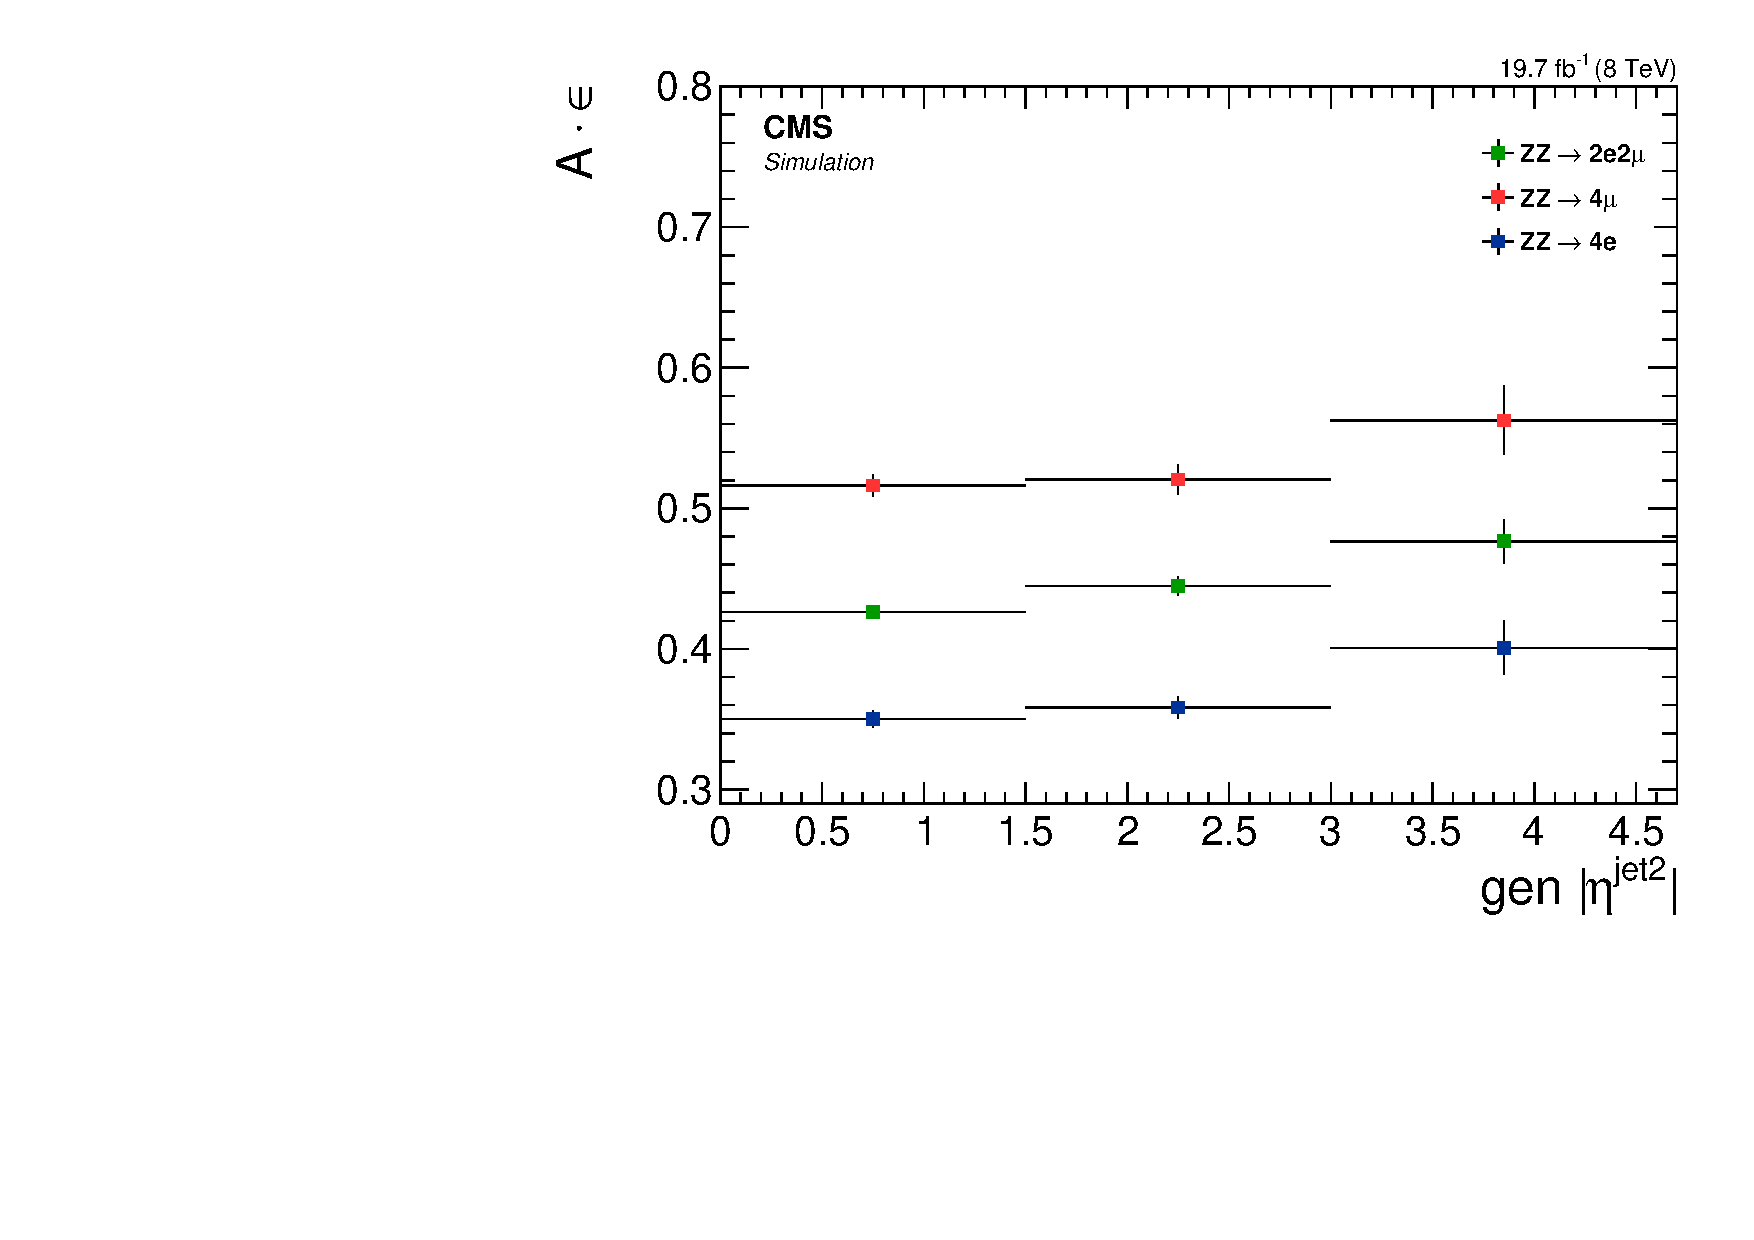
\includegraphics[width=\cmsFigWidth]{Figures/DiffAcceptance_EtaJet2_Mad}
    %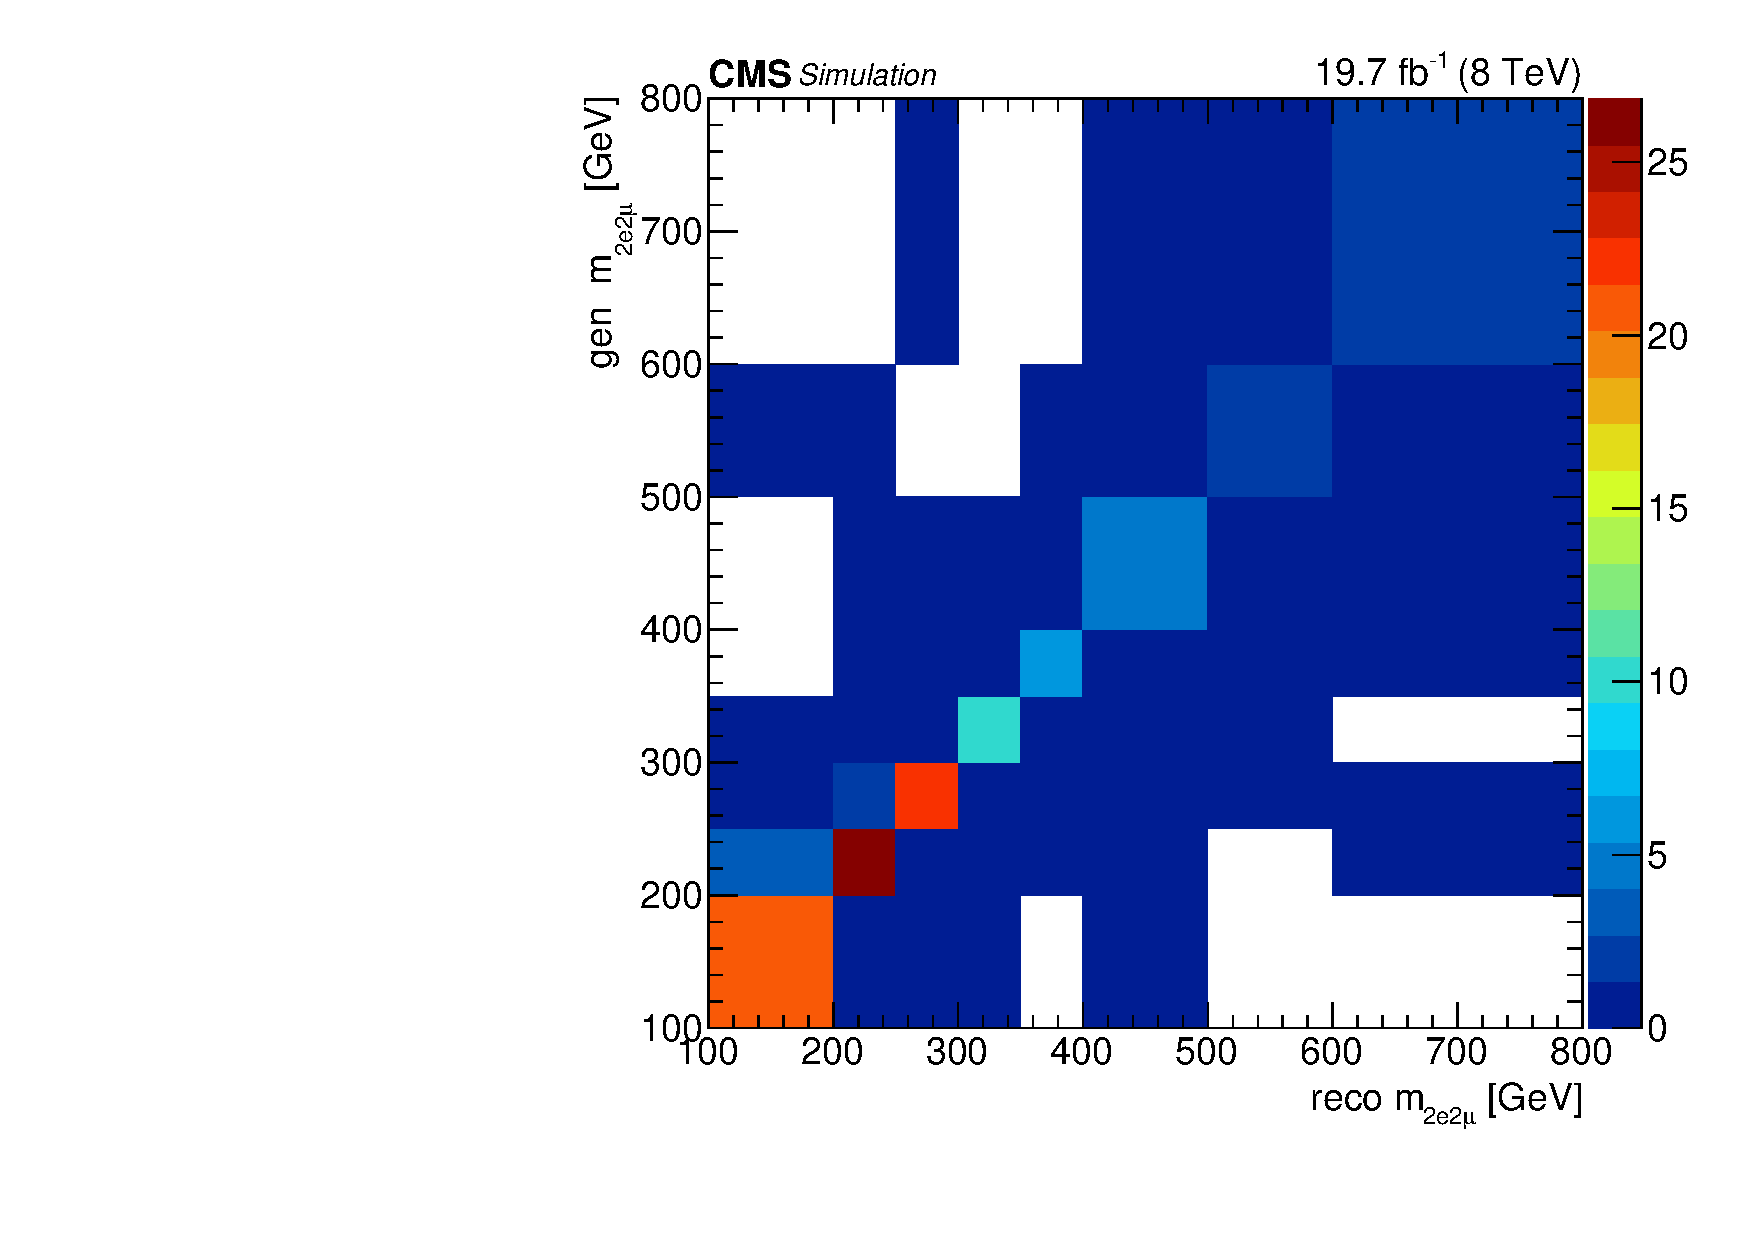
\includegraphics[width=\cmsFigWidth]{Figures/ResMat_qqggJJ_Mass_ZZTo2e2m_st_01_Pow}     
 %   to generate (a) and (b) labels under the figures, you can use subfloat, but this is not recommended: takes too much space
 %   \subfloat[]{
\includegraphics[width=0.2\textwidth]{CMS-bw-logo}}\subfloat[]{
\includegraphics[width=0.2\textwidth]{CMScol}}
    \caption{Acceptance ($A \cdot \epsilon$) computed in the wider fiducial region as a function of $p_T^{jet1}$  (top left), $p_T^{jet2}$  (top right), $\eta^{jet1}$ (bottom left) and $\eta^{jet2}$
distributions, according to the final state: 
      $4\mu$ (green), $4e$ (blue), $2e2\mu$  (red). Distributions are obtained using the  \texttt{Powheg} set of samples for  $m_{ZZ}$ and 
     the  \texttt{MadGraph} set of samples for the other variables.} 
    \label{fig:A_diff_jet}
  \end{center}
\end{figure}

\subsection{The differential ZZ cross-section measurements}
The study of vector boson pair production is important both as check of the SM and in search for new physics. 
Non-resonant $ZZ$ events are the dominant background in the $H \to ZZ \to 4\ell$ analysis and a good knowledge of 
these processes is  very useful for the study of the associated production of a $Z$ boson with the Higgs, especially at 13 TeV.
However, a lot of information
can still be extracted from data at 8 TeV, in particular as regards the associate production of a Z boson pair with jets. 
In addiction to the invariant mass of the four lepton system, the differential $ZZ$ cross-section is determined as
a function of the number of jets produced in the event, the invariant mass of the two most energetic jets ($m_{jj}$), the 
$\Delta\eta$ between them ($\Delta\eta_{jj}$), their transverse momentum and pseudorapidity (leading jet $p_{T}(\eta)^{jet1}$ and sub-leading jet $p_{T}(\eta)^{jet2}$). Both jets with  $\eta^{jet}<4.7$ and central jets with $\eta^{jet}<2.4$ are considered.\\
\\
The cross-section in each bin of each observable is determined from the event yields subtracting
the backgrounds. Each distribution is then corrected for event selection efficiencies
and for detector resolution effects in order to be compared with predictions from event generators.
The correction procedure is based on unfolding techniques, as implemented in the
\texttt{RooUnfold} toolkit~\cite{RooUnfold}, which provides both singular value decomposition (SVD)~\cite{SVD} and
the d'Agostini~\cite{DAgostini} methods. Both algorithms use a response matrix that correlates the observable
with and without detector effects. Regularization parameters can be tuned to obtain results that are robust against 
numerical instabilities and statistical fluctuations. The differential cross-section is then derived by dividing the
corrected number of events by the integrated luminosity, the branching ratio and the bin width.\\
\\
For each measured distribution, a response matrix is evaluated using two different sets of generators: the first one is composed of signal samples generated with \texttt{MadGraph} ($qq/qg/gg \to ZZ$), \texttt{MCFM} ($gg \to ZZ$) and \texttt{Phantom} ($qq \to ZZ+2jets$). The second one has the \texttt{Powheg} sample ($qq \to ZZ$) instead of
the \texttt{MadGraph} one. The \texttt{MadGraph} set is the reference set for the jet-related variables,
while the  \texttt{Powheg} one is used for check and comparison purposes. For the $m_{ZZ}$ distribution the role of the two sets of samples is switched.\\
As reported above, the signal definition of the generated events requires $60 < m_{Z_1}, m_{Z_2} < 120$  GeV. 
%  and $m_{ZZ} >$ 100 GeV. 
In order to minimize the model uncertainties due to unnecessary extrapolations of the measurement outside experimentally well-described phase space regions, cross-section distributions are also extracted in the tighter fiducial region, corresponding to the visible phase space defined by the kinematic and geometrical acceptance of leptons.\\ 
The same selection as in the inclusive cross-section measurement is applied to the reconstructed events.\\ 
Response matrices built using the reference set of samples and obtained in the tight fiducial region are 
reported in Figures~\ref{fig:Mass_matrices}-%,~\ref{fig:Jets_matrices},~\ref{fig:CentralJets_matrices},~\ref{fig:Mjj_matrices},~\ref{fig:Mjj_matrices},~\ref{fig:Deta_matrices},~\ref{fig:CentralDeta_matrices},~\ref{fig:PtJet1_matrices} and
\ref{fig:PtJet2_matrices} for each variable.\\
\begin{figure}[hbtp]
  \begin{center}
    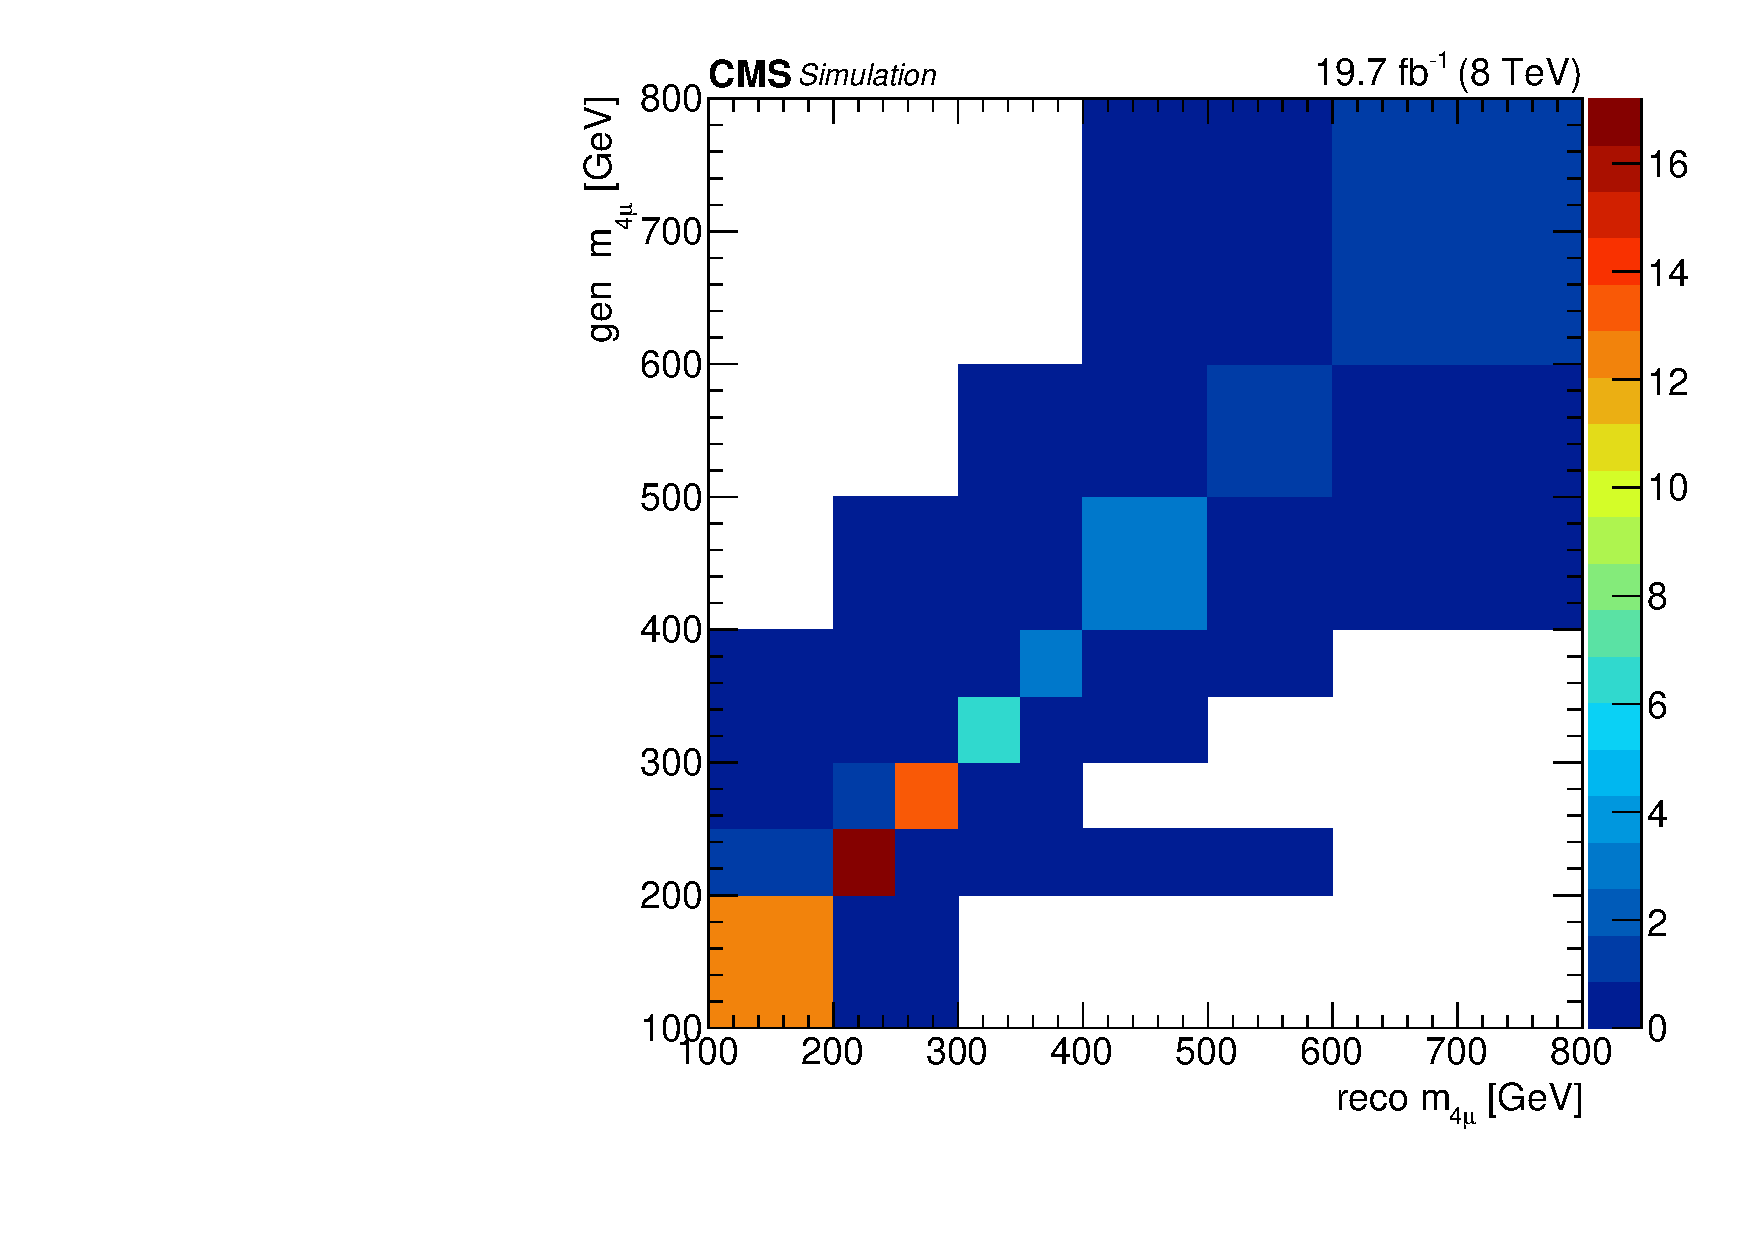
\includegraphics[width=\cmsFigWidth]{Figures/ResMat_qqggJJ_Mass_ZZTo4m_st_01_fr_Pow}
    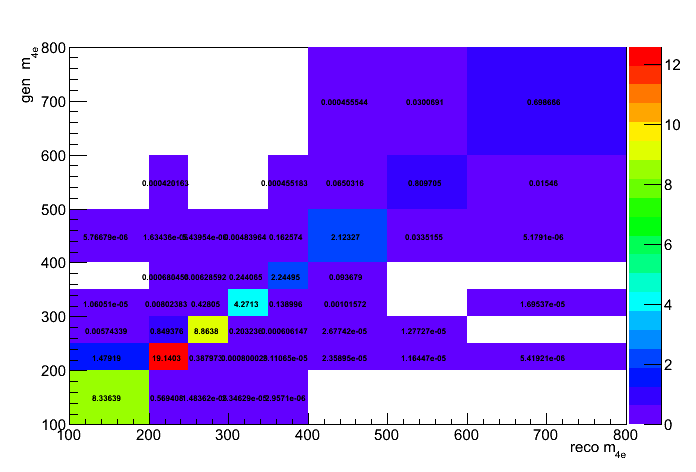
\includegraphics[width=\cmsFigWidth]{Figures/ResMat_qqggJJ_Mass_ZZTo4e_st_01_fr_Pow}
    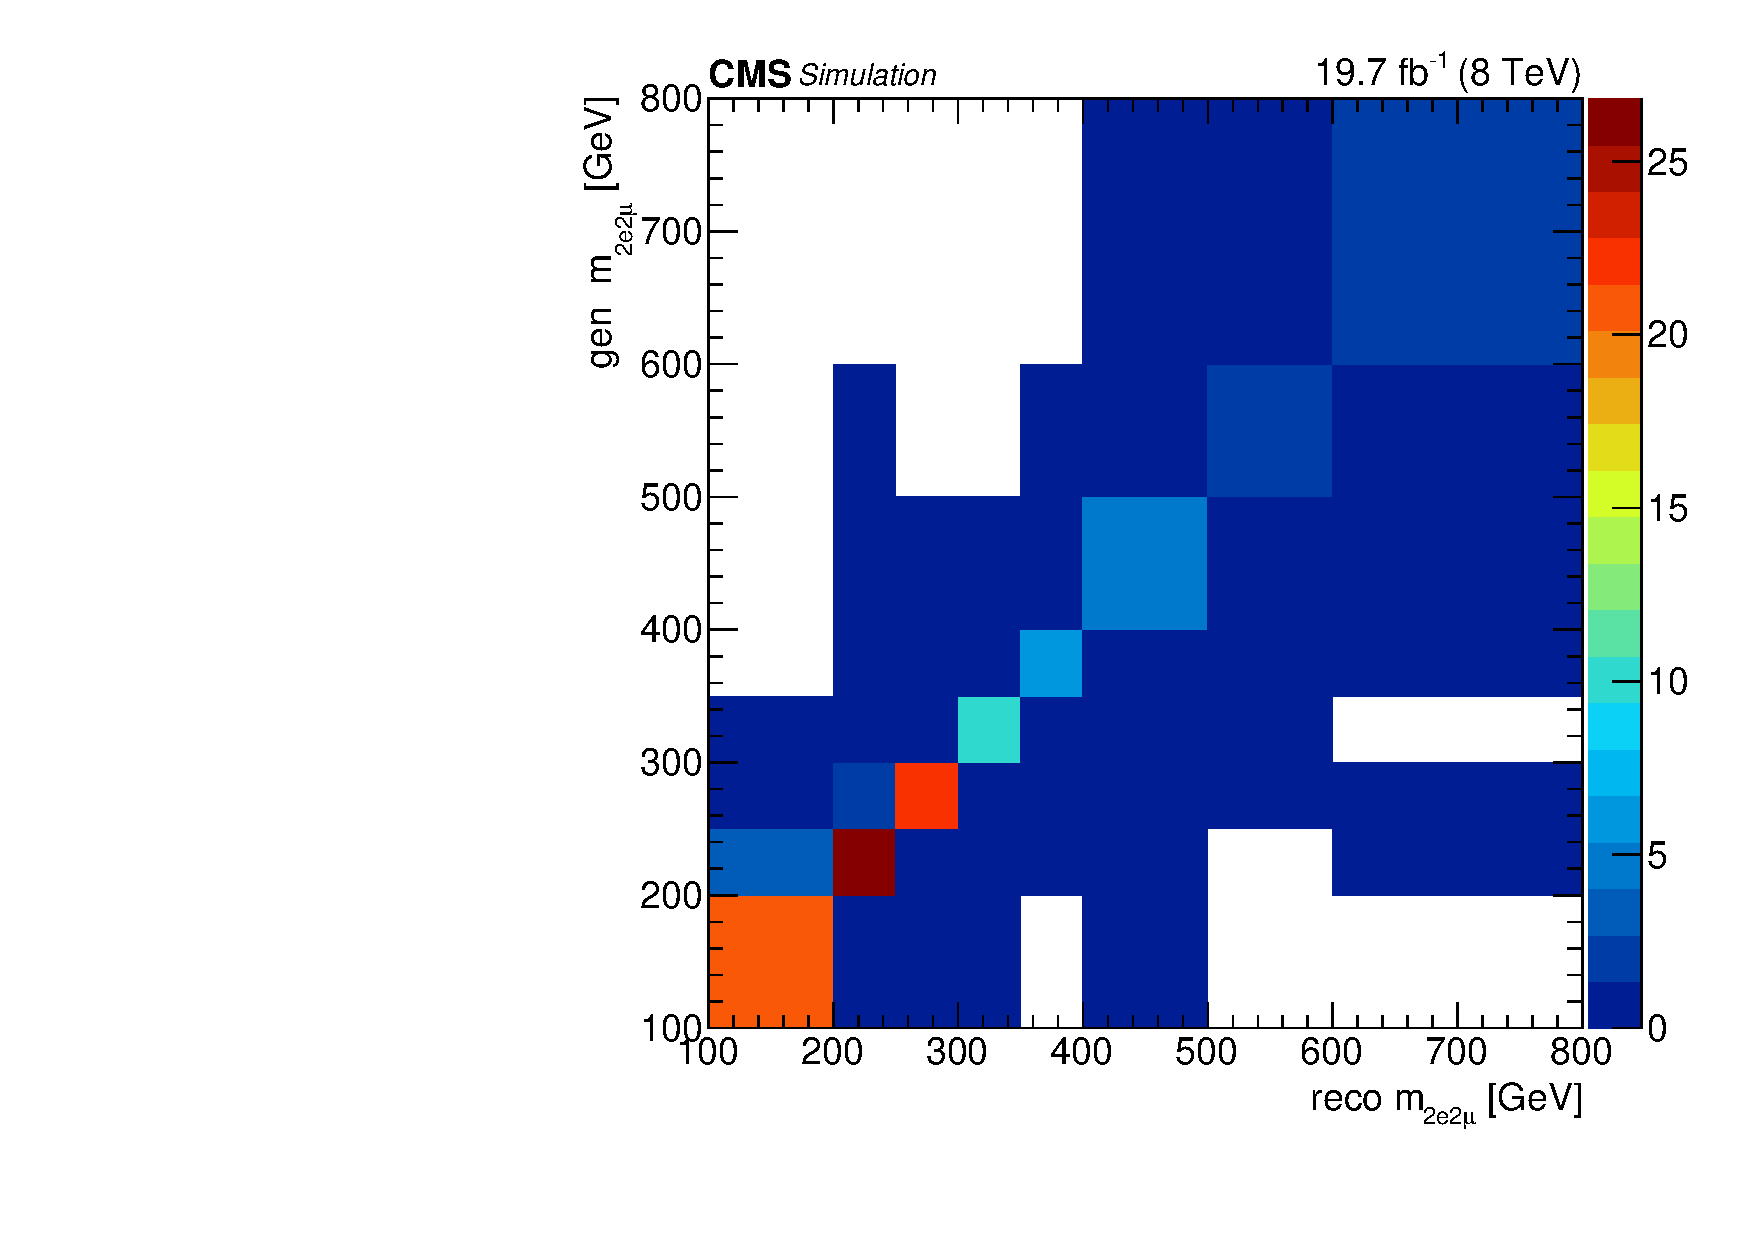
\includegraphics[width=\cmsFigWidth]{Figures/ResMat_qqggJJ_Mass_ZZTo2e2m_st_01_fr_Pow}     
 %   to generate (a) and (b) labels under the figures, you can use subfloat, but this is not recommended: takes too much space
 %   \subfloat[]{
\includegraphics[width=0.2\textwidth]{CMS-bw-logo}}\subfloat[]{
\includegraphics[width=0.2\textwidth]{CMScol}}
    \caption{Response matrices for the $m_{ZZ}$ distribution, according to the final state:  $4\mu$ (top left), $4e$ (top right), $2e2\mu$  (bottom). Matrices are obtained using the  \texttt{Powheg} set of samples. The tight fiducial region is considered.} 
    \label{fig:Mass_matrices}
  \end{center}
\end{figure}

\begin{figure}[hbtp]
  \begin{center}
    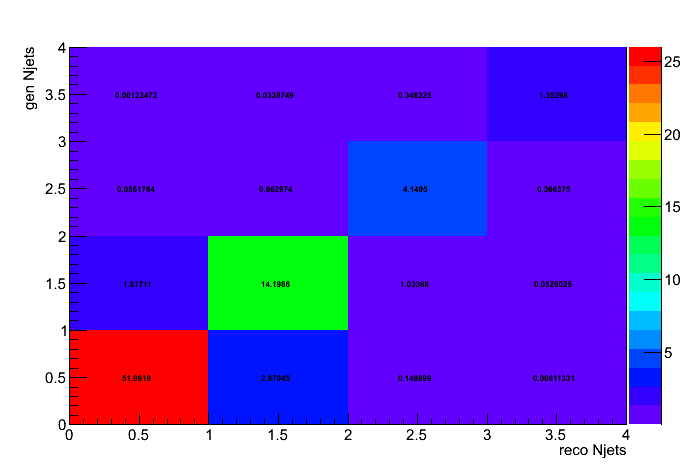
\includegraphics[width=\cmsFigWidth]{Figures/ResMat_qqggJJ_Jets_ZZTo4m_st_01_fr_Mad}
    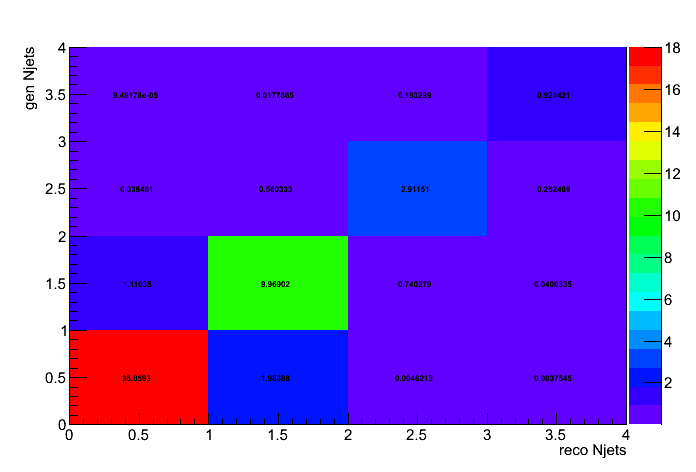
\includegraphics[width=\cmsFigWidth]{Figures/ResMat_qqggJJ_Jets_ZZTo4e_st_01_fr_Mad}
    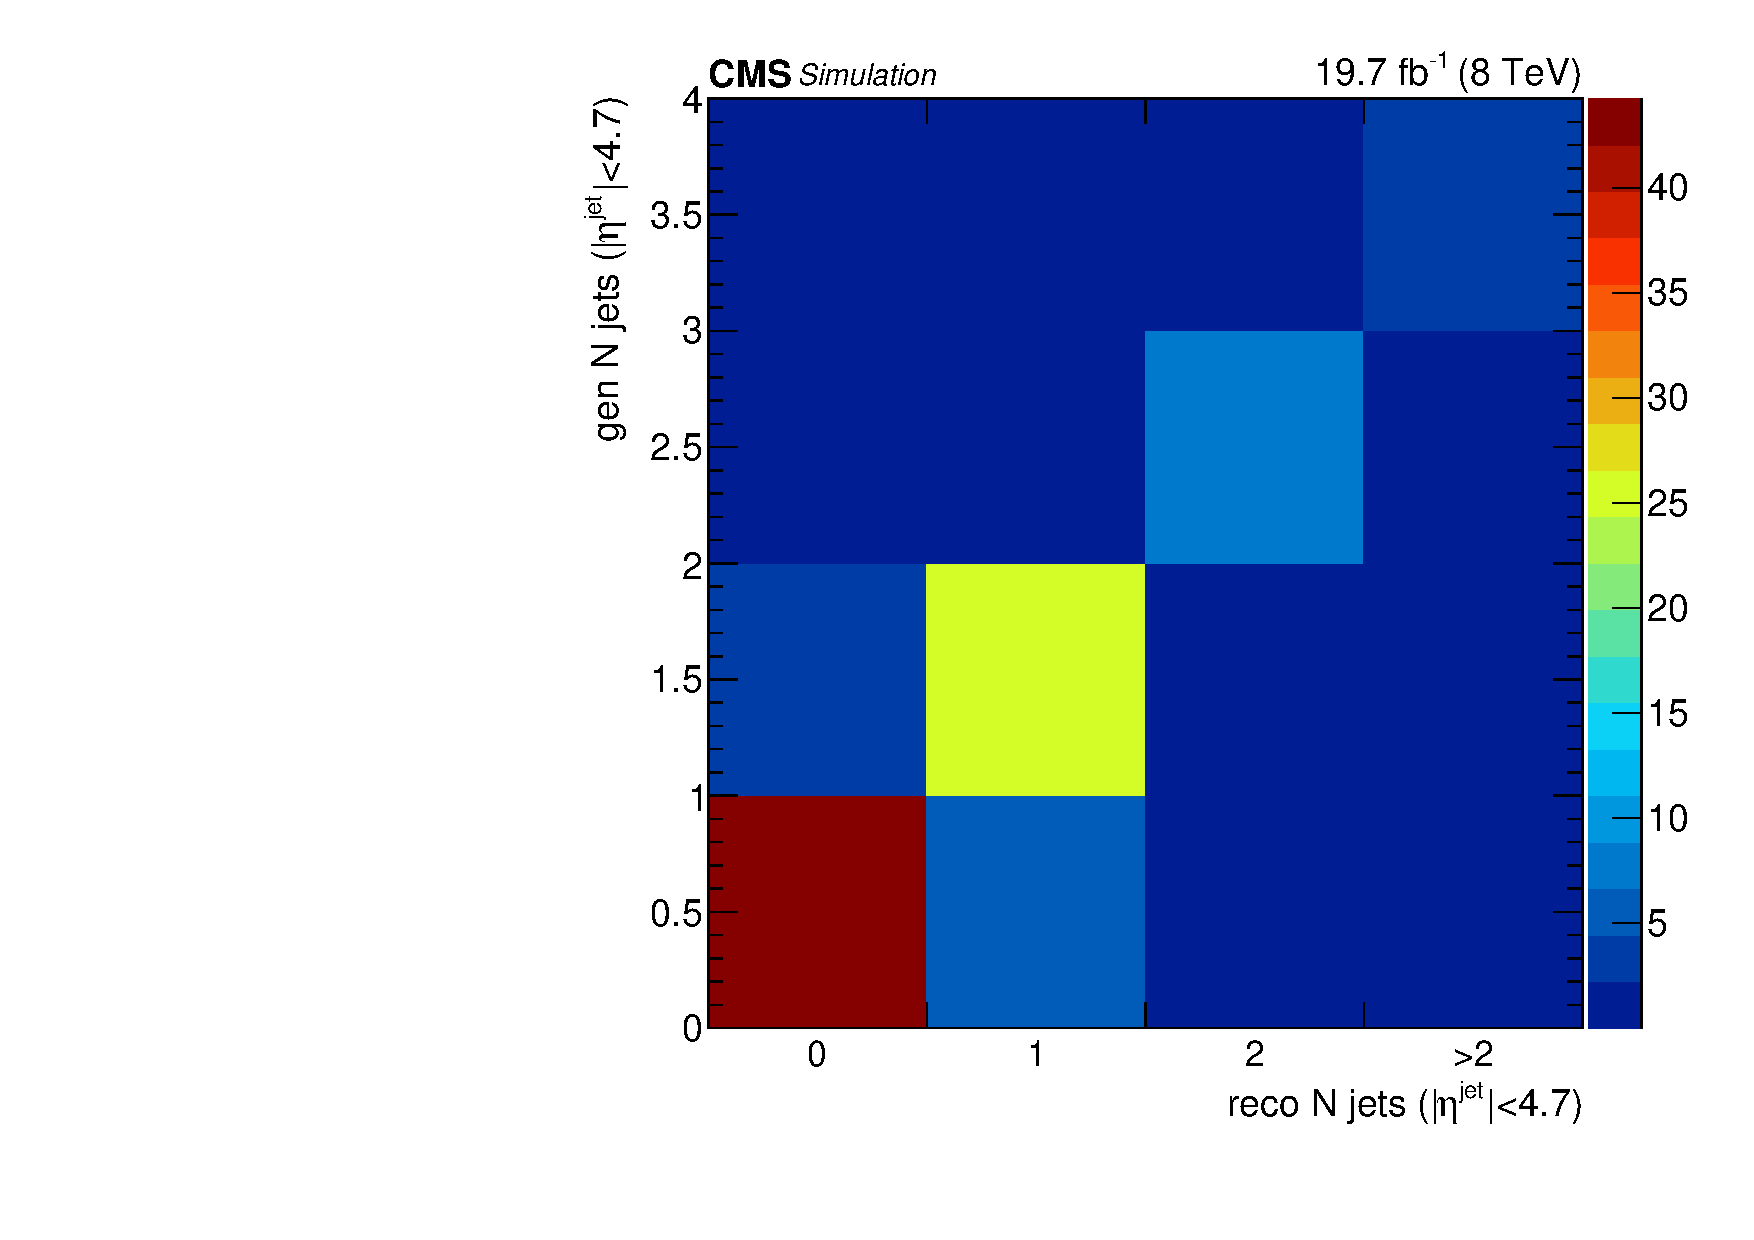
\includegraphics[width=\cmsFigWidth]{Figures/ResMat_qqggJJ_Jets_ZZTo2e2m_st_01_fr_Mad}     
 %   to generate (a) and (b) labels under the figures, you can use subfloat, but this is not recommended: takes too much space
 %   \subfloat[]{
\includegraphics[width=0.2\textwidth]{CMS-bw-logo}}\subfloat[]{\includegraphics[width=0.2\textwidth]{CMScol}}
    \caption{Response matrices for the $N\ jets$ distribution, according to the final state:  $4\mu$ (top left), $4e$ (top right), $2e2\mu$  (bottom). Matrices are obtained using the  \texttt{MadGraph} set of samples. The tight fiducial region is considered.} 
    \label{fig:Jets_matrices}
  \end{center}
\end{figure}
\begin{figure}[hbtp]
  \begin{center}
    \includegraphics[width=\cmsFigWidth]{Figures/ResMat_qqggJJ_CentralJets_ZZTo4m_st_01_fr_Mad}
    \includegraphics[width=\cmsFigWidth]{Figures/ResMat_qqggJJ_CentralJets_ZZTo4e_st_01_fr_Mad}
    \includegraphics[width=\cmsFigWidth]{Figures/ResMat_qqggJJ_CentralJets_ZZTo2e2m_st_01_fr_Mad}     
 %   to generate (a) and (b) labels under the figures, you can use subfloat, but this is not recommended: takes too much space
 %   \subfloat[]{\includegraphics[width=0.2\textwidth]{CMS-bw-logo}}\subfloat[]{\includegraphics[width=0.2\textwidth]{CMScol}}
    \caption{Response matrices for the $N\ central\ jets$ distribution (with $\eta^{jet}<2.4$) , according to the final state:  $4\mu$ (top left), $4e$ (top right), $2e2\mu$  (bottom). Matrices are obtained using the  \texttt{MadGraph} set of samples. The tight fiducial region is considered.} 
    \label{fig:CentralJets_matrices}
  \end{center}
\end{figure}
\begin{figure}[hbtp]
  \begin{center}
    \includegraphics[width=\cmsFigWidth]{Figures/ResMat_qqggJJ_Mjj_ZZTo4m_st_01_fr_Mad}
    \includegraphics[width=\cmsFigWidth]{Figures/ResMat_qqggJJ_Mjj_ZZTo4e_st_01_fr_Mad}
    \includegraphics[width=\cmsFigWidth]{Figures/ResMat_qqggJJ_Mjj_ZZTo2e2m_st_01_fr_Mad}     
 %   to generate (a) and (b) labels under the figures, you can use subfloat, but this is not recommended: takes too much space
 %   \subfloat[]{\includegraphics[width=0.2\textwidth]{CMS-bw-logo}}\subfloat[]{\includegraphics[width=0.2\textwidth]{CMScol}}
    \caption{Response matrices for the $m_{jj}$ distribution, according to the final state:  $4\mu$ (top left), $4e$ (top right), $2e2\mu$  (bottom). Matrices are obtained using the  \texttt{MadGraph} set of samples. The tight fiducial region is considered.} 
    \label{fig:Mjj_matrices}
  \end{center}
\end{figure}
\begin{figure}[hbtp]
  \begin{center}
    \includegraphics[width=\cmsFigWidth]{Figures/ResMat_qqggJJ_CentralMjj_ZZTo4m_st_01_fr_Mad}
    \includegraphics[width=\cmsFigWidth]{Figures/ResMat_qqggJJ_CentralMjj_ZZTo4e_st_01_fr_Mad}
    \includegraphics[width=\cmsFigWidth]{Figures/ResMat_qqggJJ_CentralMjj_ZZTo2e2m_st_01_fr_Mad}     
 %   to generate (a) and (b) labels under the figures, you can use subfloat, but this is not recommended: takes too much space
 %   \subfloat[]{\includegraphics[width=0.2\textwidth]{CMS-bw-logo}}\subfloat[]{\includegraphics[width=0.2\textwidth]{CMScol}}
    \caption{Response matrices for the $m_{jj}$ distribution (with $\eta^{jet}<2.4$), according to the final state:  $4\mu$ (top left), $4e$ (top right), $2e2\mu$  (bottom). Matrices are obtained using the  \texttt{MadGraph} set of samples. The tight fiducial region is considered.} 
    \label{fig:CentralMjj_matrices}
  \end{center}
\end{figure}
\begin{figure}[hbtp]
  \begin{center}
    \includegraphics[width=\cmsFigWidth]{Figures/ResMat_qqggJJ_Deta_ZZTo4m_st_01_fr_Mad}
    \includegraphics[width=\cmsFigWidth]{Figures/ResMat_qqggJJ_Deta_ZZTo4e_st_01_fr_Mad}
    \includegraphics[width=\cmsFigWidth]{Figures/ResMat_qqggJJ_Deta_ZZTo2e2m_st_01_fr_Mad}     
 %   to generate (a) and (b) labels under the figures, you can use subfloat, but this is not recommended: takes too much space
 %   \subfloat[]{\includegraphics[width=0.2\textwidth]{CMS-bw-logo}}\subfloat[]{\includegraphics[width=0.2\textwidth]{CMScol}}
    \caption{Response matrices for the $\Delta\eta_{jj}$ distribution, according to the final state:  $4\mu$ (top left), $4e$ (top right), $2e2\mu$  (bottom). Matrices are obtained using the  \texttt{MadGraph} set of samples. The tight fiducial region is considered.} 
    \label{fig:Deta_matrices}
  \end{center}
\end{figure}
\begin{figure}[hbtp]
  \begin{center}
    \includegraphics[width=\cmsFigWidth]{Figures/ResMat_qqggJJ_CentralDeta_ZZTo4m_st_01_fr_Mad}
    \includegraphics[width=\cmsFigWidth]{Figures/ResMat_qqggJJ_CentralDeta_ZZTo4e_st_01_fr_Mad}
    \includegraphics[width=\cmsFigWidth]{Figures/ResMat_qqggJJ_CentralDeta_ZZTo2e2m_st_01_fr_Mad}     
 %   to generate (a) and (b) labels under the figures, you can use subfloat, but this is not recommended: takes too much space
 %   \subfloat[]{\includegraphics[width=0.2\textwidth]{CMS-bw-logo}}\subfloat[]{\includegraphics[width=0.2\textwidth]{CMScol}}
    \caption{Response matrices for the $\Delta\eta_{jj}$ distribution (with $\eta^{jet}<2.4$), according to the final state:  $4\mu$ (top left), $4e$ (top right), $2e2\mu$  (bottom). Matrices are obtained using the  \texttt{MadGraph} set of samples. The tight fiducial region is considered.} 
    \label{fig:CentralDeta_matrices}
  \end{center}
\end{figure}
\begin{figure}[hbtp]
  \begin{center}
    \includegraphics[width=\cmsFigWidth]{Figures/ResMat_qqggJJ_PtJet1_ZZTo4m_st_01_fr_Mad}
    \includegraphics[width=\cmsFigWidth]{Figures/ResMat_qqggJJ_PtJet1_ZZTo4e_st_01_fr_Mad}
    \includegraphics[width=\cmsFigWidth]{Figures/ResMat_qqggJJ_PtJet1_ZZTo2e2m_st_01_fr_Mad}     
 %   to generate (a) and (b) labels under the figures, you can use subfloat, but this is not recommended: takes too much space
 %   \subfloat[]{\includegraphics[width=0.2\textwidth]{CMS-bw-logo}}\subfloat[]{\includegraphics[width=0.2\textwidth]{CMScol}}
    \caption{Response matrices for the $p_{T}$ distribution of the leading jet, according to the final state:  $4\mu$ (top left), $4e$ (top right), $2e2\mu$  (bottom). Matrices are obtained using the  \texttt{MadGraph} set of samples. The tight fiducial region is considered. } 
    \label{fig:PtJet1_matrices}
  \end{center}
\end{figure}
\begin{figure}[hbtp]
  \begin{center}
    \includegraphics[width=\cmsFigWidth]{Figures/ResMat_qqggJJ_PtJet2_ZZTo4m_st_01_fr_Mad}
    \includegraphics[width=\cmsFigWidth]{Figures/ResMat_qqggJJ_PtJet2_ZZTo4e_st_01_fr_Mad}
    \includegraphics[width=\cmsFigWidth]{Figures/ResMat_qqggJJ_PtJet2_ZZTo2e2m_st_01_fr_Mad}     
 %   to generate (a) and (b) labels under the figures, you can use subfloat, but this is not recommended: takes too much space
 %   \subfloat[]{\includegraphics[width=0.2\textwidth]{CMS-bw-logo}}\subfloat[]{\includegraphics[width=0.2\textwidth]{CMScol}}
    \caption{Response matrices for the $p_{T}$ distribution of the sub-leading jet, according to the final state:  $4\mu$ (top left), $4e$ (top right), $2e2\mu$  (bottom). Matrices are obtained using the  \texttt{MadGraph} set of samples. The tight fiducial region is considered.} 
    \label{fig:PtJet2_matrices}
  \end{center}
\end{figure}

\begin{figure}[hbtp]
  \begin{center}
    \includegraphics[width=\cmsFigWidth]{Figures/ResMat_qqggJJ_EtaJet1_ZZTo4m_st_01_fr_Mad}
    \includegraphics[width=\cmsFigWidth]{Figures/ResMat_qqggJJ_EtaJet1_ZZTo4e_st_01_fr_Mad}
    \includegraphics[width=\cmsFigWidth]{Figures/ResMat_qqggJJ_EtaJet1_ZZTo2e2m_st_01_fr_Mad}     
 %   to generate (a) and (b) labels under the figures, you can use subfloat, but this is not recommended: takes too much space
 %   \subfloat[]{\includegraphics[width=0.2\textwidth]{CMS-bw-logo}}\subfloat[]{\includegraphics[width=0.2\textwidth]{CMScol}}
    \caption{Response matrices for the $\eta$ distribution of the leading jet, according to the final state:  $4\mu$ (top left), $4e$ (top right), $2e2\mu$  (bottom). Matrices are obtained using the  \texttt{MadGraph} set of samples. The tight fiducial region is considered.} 
    \label{fig:EtaJet1_matrices}
  \end{center}
\end{figure}
\begin{figure}[hbtp]
  \begin{center}
    \includegraphics[width=\cmsFigWidth]{Figures/ResMat_qqggJJ_EtaJet2_ZZTo4m_st_01_fr_Mad}
    \includegraphics[width=\cmsFigWidth]{Figures/ResMat_qqggJJ_EtaJet2_ZZTo4e_st_01_fr_Mad}
    \includegraphics[width=\cmsFigWidth]{Figures/ResMat_qqggJJ_EtaJet2_ZZTo2e2m_st_01_fr_Mad}     
 %   to generate (a) and (b) labels under the figures, you can use subfloat, but this is not recommended: takes too much space
 %   \subfloat[]{\includegraphics[width=0.2\textwidth]{CMS-bw-logo}}\subfloat[]{\includegraphics[width=0.2\textwidth]{CMScol}}
    \caption{Response matrices for the $\eta$ distribution of the sub-leading jet, according to the final state:  $4\mu$ (top left), $4e$ (top right), $2e2\mu$  (bottom). Matrices are obtained using the  \texttt{MadGraph} set of samples. The tight fiducial region is considered.} 
    \label{fig:EtaJet2_matrices}
  \end{center}
\end{figure}
\clearpage

\begin{figure}[hbtp]
  \begin{center}
    \includegraphics[width=\cmsFigWidth]{Figures/Mass_ZZTo4m_Pow_fr_binwidth}
    \includegraphics[width=\cmsFigWidth]{Figures/Mass_ZZTo4e_Pow_fr_binwidth}
    \includegraphics[width=\cmsFigWidth]{Figures/Mass_ZZTo2e2m_Pow_fr_binwidth}  
    \includegraphics[width=\cmsFigWidth]{Figures/Mass_ZZTo4l_Pow_fr}    
 %   to generate (a) and (b) labels under the figures, you can use subfloat, but this is not recommended: takes too much space
 %   \subfloat[]{\includegraphics[width=0.2\textwidth]{CMS-bw-logo}}\subfloat[]{\includegraphics[width=0.2\textwidth]{CMScol}}
    \caption{\footnotesize{Data (red), unfolded data (blue), generated (dashed blue) and MC reconstructed (dashed red) $m_{ZZ}$ distributions, according to the final state: 
$4\mu$ (top left), $4e$ (top right), $2e2\mu$  (bottom left),  $4\ell$ (bottom right). The unfolded distributions are obtained  in the tight fiducial region using the SVD algorithm, with $k_{reg} = 4$, and compared to predictions from the \texttt{Powheg} set of samples.}} 
    \label{fig:Mass_unfolding}
  \end{center}
\end{figure}

\begin{figure}[hbtp]
  \begin{center}
    \includegraphics[width=\cmsFigWidth]{Figures/Jets_ZZTo4m_Mad_fr_binwidth}
    \includegraphics[width=\cmsFigWidth]{Figures/Jets_ZZTo4e_Mad_fr_binwidth}
    \includegraphics[width=\cmsFigWidth]{Figures/Jets_ZZTo2e2m_Mad_fr_binwidth}     
    \includegraphics[width=\cmsFigWidth]{Figures/Jets_ZZTo4l_Mad_fr}    
 %   to generate (a) and (b) labels under the figures, you can use subfloat, but this is not recommended: takes too much space
 %   \subfloat[]{\includegraphics[width=0.2\textwidth]{CMS-bw-logo}}\subfloat[]{\includegraphics[width=0.2\textwidth]{CMScol}}
    \caption{\footnotesize{Data (red), unfolded data (blue), generated (dashed blue) and MC reconstructed (dashed red) $N\ jets$ distributions, according to the final state: (top left) $4\mu$, (top right) $4e$, (bottom left) $2e2\mu$, (bottom right) $4\ell$. The unfolded distributions are obtained in the tight fiducial region using the D'Agostini algorithm, with 4 iterations, and compared to predictions from the \texttt{MadGraph} set of samples.}} 
    \label{fig:Jets_unfolding}
  \end{center}
\end{figure}

\begin{figure}[hbtp]
  \begin{center}
    \includegraphics[width=\cmsFigWidth]{Figures/CentralJets_ZZTo4m_Mad_fr_binwidth}
    \includegraphics[width=\cmsFigWidth]{Figures/CentralJets_ZZTo4e_Mad_fr_binwidth}
    \includegraphics[width=\cmsFigWidth]{Figures/CentralJets_ZZTo2e2m_Mad_fr_binwidth}     
    \includegraphics[width=\cmsFigWidth]{Figures/CentralJets_ZZTo4l_Mad_fr}    
 %   to generate (a) and (b) labels under the figures, you can use subfloat, but this is not recommended: takes too much space
 %   \subfloat[]{\includegraphics[width=0.2\textwidth]{CMS-bw-logo}}\subfloat[]{\includegraphics[width=0.2\textwidth]{CMScol}}
    \caption{\footnotesize{Data (red), unfolded data (blue), generated (dashed blue) and MC reconstructed (dashed red) $N\ central\ jets$ distributions, according to the final state: (top left) $4\mu$, (top right) $4e$, (bottom left) $2e2\mu$, (bottom right) $4\ell$. The unfolded distributions are obtained in the tight fiducial region using the D'Agostini algorithm, with 4 iterations, and compared to predictions from the \texttt{MadGraph} set of samples.}} 
    \label{fig:CentralJets_unfolding}
  \end{center}
\end{figure}
%\clearpage
\begin{figure}[hbtp]
  \begin{center}
    \includegraphics[width=\cmsFigWidth]{Figures/Mjj_ZZTo4m_Mad_fr_binwidth}
    \includegraphics[width=\cmsFigWidth]{Figures/Mjj_ZZTo4e_Mad_fr_binwidth}
    \includegraphics[width=\cmsFigWidth]{Figures/Mjj_ZZTo2e2m_Mad_fr_binwidth}   
    \includegraphics[width=\cmsFigWidth]{Figures/Mjj_ZZTo4l_Mad_fr}      
 %   to generate (a) and (b) labels under the figures, you can use subfloat, but this is not recommended: takes too much space
 %   \subfloat[]{\includegraphics[width=0.2\textwidth]{CMS-bw-logo}}\subfloat[]{\includegraphics[width=0.2\textwidth]{CMScol}}
    \caption{\footnotesize{Data (red), unfolded data (blue), generated (dashed blue) and MC reconstructed (dashed red) $m_{jj}$ distributions, according to the final state: (top left) $4\mu$, (top right) $4e$, (bottom left) $2e2\mu$, (bottom right) $4\ell$. The unfolded distributions are obtained in the tight fiducial region using the D'Agostini algorithm, with 4 iterations, and compared to predictions from the \texttt{MadGraph} set of samples.}} 
    \label{fig:Mjj_unfolding}
  \end{center}
\end{figure}
\begin{figure}[hbtp]
  \begin{center}
    \includegraphics[width=\cmsFigWidth]{Figures/CentralMjj_ZZTo4m_Mad_fr_binwidth}
    \includegraphics[width=\cmsFigWidth]{Figures/CentralMjj_ZZTo4e_Mad_fr_binwidth}
    \includegraphics[width=\cmsFigWidth]{Figures/CentralMjj_ZZTo2e2m_Mad_fr_binwidth}   
    \includegraphics[width=\cmsFigWidth]{Figures/CentralMjj_ZZTo4l_Mad_fr}      
 %   to generate (a) and (b) labels under the figures, you can use subfloat, but this is not recommended: takes too much space
 %   \subfloat[]{\includegraphics[width=0.2\textwidth]{CMS-bw-logo}}\subfloat[]{\includegraphics[width=0.2\textwidth]{CMScol}}
    \caption{\footnotesize{Data (red), unfolded data (blue), generated (dashed blue) and MC reconstructed (dashed red) $m_{jj}$ distributions (using central jets with $\eta^{jet}<2.4$), according to the final state: (top left) $4\mu$, (top right) $4e$, (bottom left) $2e2\mu$, (bottom right) $4\ell$. The unfolded distributions are obtained in the tight fiducial region using the D'Agostini algorithm, with 4 iterations, and compared to predictions from the \texttt{MadGraph} set of samples.}} 
    \label{fig:CentralMjj_unfolding}
  \end{center}
\end{figure}

\begin{figure}[hbtp]
  \begin{center}
    \includegraphics[width=\cmsFigWidth]{Figures/Deta_ZZTo4m_Mad_fr_binwidth}
    \includegraphics[width=\cmsFigWidth]{Figures/Deta_ZZTo4e_Mad_fr_binwidth}
    \includegraphics[width=\cmsFigWidth]{Figures/Deta_ZZTo2e2m_Mad_fr_binwidth}  
    \includegraphics[width=\cmsFigWidth]{Figures/Deta_ZZTo4l_Mad_fr}       
 %   to generate (a) and (b) labels under the figures, you can use subfloat, but this is not recommended: takes too much space
 %   \subfloat[]{\includegraphics[width=0.2\textwidth]{CMS-bw-logo}}\subfloat[]{\includegraphics[width=0.2\textwidth]{CMScol}}
    \caption{\footnotesize{Data (red), unfolded data (blue), generated (dashed blue) and MC reconstructed (dashed red) $\Delta\eta_{jj}$ distributions, according to the final state: (top left) $4\mu$, (top right) $4e$, (bottom left) $2e2\mu$, (bottom right) $4\ell$. The unfolded distributions are obtained in the tight fiducial region using the D'Agostini algorithm, with 4 iterations, and compared to predictions from the \texttt{MadGraph} set of samples.}} 
    \label{fig:Deta_unfolding}
  \end{center}
\end{figure}
\begin{figure}[hbtp]
  \begin{center}
    \includegraphics[width=\cmsFigWidth]{Figures/CentralDeta_ZZTo4m_Mad_fr_binwidth}
    \includegraphics[width=\cmsFigWidth]{Figures/CentralDeta_ZZTo4e_Mad_fr_binwidth}
    \includegraphics[width=\cmsFigWidth]{Figures/CentralDeta_ZZTo2e2m_Mad_fr_binwidth}  
    \includegraphics[width=\cmsFigWidth]{Figures/CentralDeta_ZZTo4l_Mad_fr}       
 %   to generate (a) and (b) labels under the figures, you can use subfloat, but this is not recommended: takes too much space
 %   \subfloat[]{\includegraphics[width=0.2\textwidth]{CMS-bw-logo}}\subfloat[]{\includegraphics[width=0.2\textwidth]{CMScol}}
    \caption{\footnotesize{Data (red), unfolded data (blue), generated (dashed blue) and MC reconstructed (dashed red) $\Delta\eta_{jj}$ distributions (using central jets with $\eta^{jet}<2.4$), according to the final state: (top left) $4\mu$, (top right) $4e$, (bottom left) $2e2\mu$, (bottom right) $4\ell$. The unfolded distributions are obtained in the tight fiducial region using the D'Agostini algorithm, with 4 iterations, and compared to predictions from the \texttt{MadGraph} set of samples.}} 
    \label{fig:CentralDeta_unfolding}
  \end{center}
\end{figure}

\begin{figure}[hbtp]
  \begin{center}
    \includegraphics[width=\cmsFigWidth]{Figures/PtJet1_ZZTo4m_Mad_fr_binwidth}
    \includegraphics[width=\cmsFigWidth]{Figures/PtJet1_ZZTo4e_Mad_fr_binwidth}
    \includegraphics[width=\cmsFigWidth]{Figures/PtJet1_ZZTo2e2m_Mad_fr_binwidth}  
    \includegraphics[width=\cmsFigWidth]{Figures/PtJet1_ZZTo4l_Mad_fr}       
 %   to generate (a) and (b) labels under the figures, you can use subfloat, but this is not recommended: takes too much space
 %   \subfloat[]{\includegraphics[width=0.2\textwidth]{CMS-bw-logo}}\subfloat[]{\includegraphics[width=0.2\textwidth]{CMScol}}
    \caption{\footnotesize{Data (red), unfolded data (blue), generated (dashed blue) and MC reconstructed (dashed red) $p_{T}^{jet1}$ distributions, according to the final state: (top left) $4\mu$, (top right) $4e$, (bottom left) $2e2\mu$, (bottom right) $4\ell$. The unfolded distributions are obtained in the tight fiducial region using the D'Agostini algorithm, with 4 iterations, and compared to predictions from the \texttt{MadGraph} set of samples.}} 
    \label{fig:PtJet1_unfolding}
  \end{center}
\end{figure}

\begin{figure}[hbtp]
  \begin{center}
    \includegraphics[width=\cmsFigWidth]{Figures/PtJet2_ZZTo4m_Mad_fr_binwidth}
    \includegraphics[width=\cmsFigWidth]{Figures/PtJet2_ZZTo4e_Mad_fr_binwidth}
    \includegraphics[width=\cmsFigWidth]{Figures/PtJet2_ZZTo2e2m_Mad_fr_binwidth}  
    \includegraphics[width=\cmsFigWidth]{Figures/PtJet2_ZZTo4l_Mad_fr}       
 %   to generate (a) and (b) labels under the figures, you can use subfloat, but this is not recommended: takes too much space
 %   \subfloat[]{\includegraphics[width=0.2\textwidth]{CMS-bw-logo}}\subfloat[]{\includegraphics[width=0.2\textwidth]{CMScol}}
    \caption{\footnotesize{Data (red), unfolded data (blue), generated (dashed blue) and MC reconstructed (dashed red) $p_{T}^{jet2}$ distributions, according to the final state: (top left) $4\mu$, (top right) $4e$, (bottom left) $2e2\mu$, (bottom right) $4\ell$. The unfolded distributions are obtained in the tight fiducial region using the D'Agostini algorithm, with 4 iterations, and compared to predictions from the \texttt{MadGraph} set of samples.}} 
    \label{fig:PtJet2_unfolding}
  \end{center}
\end{figure}


\begin{figure}[hbtp]
  \begin{center}
    \includegraphics[width=\cmsFigWidth]{Figures/EtaJet1_ZZTo4m_Mad_fr_binwidth}
    \includegraphics[width=\cmsFigWidth]{Figures/EtaJet1_ZZTo4e_Mad_fr_binwidth}
    \includegraphics[width=\cmsFigWidth]{Figures/EtaJet1_ZZTo2e2m_Mad_fr_binwidth}  
    \includegraphics[width=\cmsFigWidth]{Figures/EtaJet1_ZZTo4l_Mad_fr}       
 %   to generate (a) and (b) labels under the figures, you can use subfloat, but this is not recommended: takes too much space
 %   \subfloat[]{\includegraphics[width=0.2\textwidth]{CMS-bw-logo}}\subfloat[]{\includegraphics[width=0.2\textwidth]{CMScol}}
    \caption{\footnotesize{Data (red), unfolded data (blue), generated (dashed blue) and MC reconstructed (dashed red) $\eta^{jet1}$ distributions, according to the final state: (top left) $4\mu$, (top right) $4e$, (bottom left) $2e2\mu$, (bottom right) $4\ell$. The unfolded distributions are obtained in the tight fiducial region using the D'Agostini algorithm, with 4 iterations, and compared to predictions from the \texttt{MadGraph} set of samples.}} 
    \label{fig:EtaJet1_unfolding}
  \end{center}
\end{figure}

\begin{figure}[hbtp]
  \begin{center}
    \includegraphics[width=\cmsFigWidth]{Figures/EtaJet2_ZZTo4m_Mad_fr_binwidth}
    \includegraphics[width=\cmsFigWidth]{Figures/EtaJet2_ZZTo4e_Mad_fr_binwidth}
    \includegraphics[width=\cmsFigWidth]{Figures/EtaJet2_ZZTo2e2m_Mad_fr_binwidth}  
    \includegraphics[width=\cmsFigWidth]{Figures/EtaJet2_ZZTo4l_Mad_fr}       
 %   to generate (a) and (b) labels under the figures, you can use subfloat, but this is not recommended: takes too much space
 %   \subfloat[]{\includegraphics[width=0.2\textwidth]{CMS-bw-logo}}\subfloat[]{\includegraphics[width=0.2\textwidth]{CMScol}}
    \caption{\footnotesize{Data (red), unfolded data (blue), generated (dashed blue) and MC reconstructed (dashed red) $\eta^{jet2}$ distributions, according to the final state: (top left) $4\mu$, (top right) $4e$, (bottom left) $2e2\mu$, (bottom right) $4\ell$. The unfolded distributions are obtained in the tight fiducial region using the D'Agostini algorithm, with 4 iterations, and compared to predictions from the \texttt{MadGraph} set of samples.}} 
    \label{fig:EtaJet2_unfolding}
  \end{center}
\end{figure}
\clearpage
\begin{figure}[hbtp]
  \begin{center}
    \includegraphics[width=\cmsFigWidth]{Figures/DiffCrossSecZZTo4mMass_Unfolded_fr_Powheg_norm.png}     
    \includegraphics[width=\cmsFigWidth]{Figures/DiffCrossSecZZTo4eMass_Unfolded_fr_Powheg_norm.png}     
    \includegraphics[width=\cmsFigWidth]{Figures/DiffCrossSecZZTo2e2mMass_Unfolded_fr_Powheg_norm.png}       
    \includegraphics[width=\cmsFigWidth]{Figures/DiffCrossSecZZTo4lMass_Unfolded_fr_Powheg_norm.png}       
 %   to generate (a) and (b) labels under the figures, you can use subfloat, but this is not recommended: takes too much space
 %   \subfloat[]{\includegraphics[width=0.2\textwidth]{CMS-bw-logo}}\subfloat[]{\includegraphics[width=0.2\textwidth]{CMScol}}%
    \caption{\footnotesize{Normalized differential cross-sections as a function of the  invariant mass of the 4 lepton system, according to the final state: $4\mu$ (top left), $4e$ (top right), $2e2\mu$  (bottom left),  $4\ell$ (bottom right). Cross-sections are extracted in the tight fiducial region and compared to predictions from the \texttt{Powheg}, \texttt{MadGraph} and \texttt{MadGraph5\_aMCatNLO} sets of samples.}}
    \label{fig:diff_xs_mass}
  \end{center}
\end{figure}

\begin{figure}[hbtp]
  \begin{center}
    \includegraphics[width=\cmsFigWidth]{Figures/DiffCrossSecZZTo4mJets_Unfolded_fr_MadGraph_norm.png}     
    \includegraphics[width=\cmsFigWidth]{Figures/DiffCrossSecZZTo4eJets_Unfolded_fr_MadGraph_norm.png}     
    \includegraphics[width=\cmsFigWidth]{Figures/DiffCrossSecZZTo2e2mJets_Unfolded_fr_MadGraph_norm.png}       
    \includegraphics[width=\cmsFigWidth]{Figures/DiffCrossSecZZTo4lJets_Unfolded_fr_MadGraph_norm.png}       
 %   to generate (a) and (b) labels under the figures, you can use subfloat, but this is not recommended: takes too much space
 %   \subfloat[]{\includegraphics[width=0.2\textwidth]{CMS-bw-logo}}\subfloat[]{\includegraphics[width=0.2\textwidth]{CMScol}}
    \caption{\footnotesize{Normalized differential cross-sections as a function of the number of jets in the event, according to the final state: $4\mu$ (top left), $4e$ (top right), $2e2\mu$  (bottom left),  $4\ell$ (bottom right). Cross-sections are extracted in the tight fiducial region and compared to predictions from the \texttt{MadGraph}, \texttt{Powheg} and \texttt{MadGraph5\_aMCatNLO} sets of samples.}}
    \label{fig:diff_xs_jets}
  \end{center}
\end{figure}

\begin{figure}[hbtp]
  \begin{center}
    \includegraphics[width=\cmsFigWidth]{Figures/DiffCrossSecZZTo4mCentralJets_Unfolded_fr_MadGraph_norm.png}     
    \includegraphics[width=\cmsFigWidth]{Figures/DiffCrossSecZZTo4eCentralJets_Unfolded_fr_MadGraph_norm.png}     
    \includegraphics[width=\cmsFigWidth]{Figures/DiffCrossSecZZTo2e2mCentralJets_Unfolded_fr_MadGraph_norm.png}       
    \includegraphics[width=\cmsFigWidth]{Figures/DiffCrossSecZZTo4lCentralJets_Unfolded_fr_MadGraph_norm.png}       
 %   to generate (a) and (b) labels under the figures, you can use subfloat, but this is not recommended: takes too much space
 %   \subfloat[]{\includegraphics[width=0.2\textwidth]{CMS-bw-logo}}\subfloat[]{\includegraphics[width=0.2\textwidth]{CMScol}}
    \caption{\footnotesize{Normalized differential cross-sections as a function of the number of central jets in the event, according to the final state: $4\mu$ (top left), $4e$ (top right), $2e2\mu$  (bottom left),  $4\ell$ (bottom right). Cross-sections are extracted in the tight fiducial region and compared to predictions from the \texttt{MadGraph}, \texttt{Powheg}  and \texttt{MadGraph5\_aMCatNLO} sets of samples.}}
    \label{fig:diff_xs_centraljets}
  \end{center}
\end{figure}

\begin{figure}[hbtp]
  \begin{center}
    \includegraphics[width=\cmsFigWidth]{Figures/DiffCrossSecZZTo4mMjj_Unfolded_fr_MadGraph_norm.png}     
    \includegraphics[width=\cmsFigWidth]{Figures/DiffCrossSecZZTo4eMjj_Unfolded_fr_MadGraph_norm.png}     
    \includegraphics[width=\cmsFigWidth]{Figures/DiffCrossSecZZTo2e2mMjj_Unfolded_fr_MadGraph_norm.png}       
    \includegraphics[width=\cmsFigWidth]{Figures/DiffCrossSecZZTo4lMjj_Unfolded_fr_MadGraph_norm.png}       
 %   to generate (a) and (b) labels under the figures, you can use subfloat, but this is not recommended: takes too much space
 %   \subfloat[]{\includegraphics[width=0.2\textwidth]{CMS-bw-logo}}\subfloat[]{\includegraphics[width=0.2\textwidth]{CMScol}}
    \caption{\footnotesize{Normalized differential cross-sections as a function of the invariant mass of the most energetic jets in the event, according to the final state: $4\mu$ (top left), $4e$ (top right), $2e2\mu$  (bottom left),  $4\ell$ (bottom right). Cross-sections are extracted in the tight fiducial region and compared to predictions from the \texttt{MadGraph}, \texttt{Powheg} and \texttt{MadGraph5\_aMCatNLO} sets of samples.}}
    \label{fig:diff_xs_mjj}
  \end{center}
\end{figure}

\begin{figure}[hbtp]
  \begin{center}
    \includegraphics[width=\cmsFigWidth]{Figures/DiffCrossSecZZTo4mCentralMjj_Unfolded_fr_MadGraph_norm.png}     
    \includegraphics[width=\cmsFigWidth]{Figures/DiffCrossSecZZTo4eCentralMjj_Unfolded_fr_MadGraph_norm.png}     
    \includegraphics[width=\cmsFigWidth]{Figures/DiffCrossSecZZTo2e2mCentralMjj_Unfolded_fr_MadGraph_norm.png}       
    \includegraphics[width=\cmsFigWidth]{Figures/DiffCrossSecZZTo4lCentralMjj_Unfolded_fr_MadGraph_norm.png}       
 %   to generate (a) and (b) labels under the figures, you can use subfloat, but this is not recommended: takes too much space
 %   \subfloat[]{\includegraphics[width=0.2\textwidth]{CMS-bw-logo}}\subfloat[]{\includegraphics[width=0.2\textwidth]{CMScol}}
    \caption{\footnotesize{Normalized differential cross-sections as a function of the invariant mass of the most energetic central jets in the event, according to the final state: $4\mu$ (top left), $4e$ (top right), $2e2\mu$  (bottom left),  $4\ell$ (bottom right). Cross-sections are extracted in the tight fiducial region and compared to predictions from the \texttt{MadGraph}, \texttt{Powheg} and \texttt{MadGraph5\_aMCatNLO} sets of samples.}}
    \label{fig:diff_xs_centralmjj}
  \end{center}
\end{figure}

\begin{figure}[hbtp]
  \begin{center}
    \includegraphics[width=\cmsFigWidth]{Figures/DiffCrossSecZZTo4mDeta_Unfolded_fr_MadGraph_norm.png}     
    \includegraphics[width=\cmsFigWidth]{Figures/DiffCrossSecZZTo4eDeta_Unfolded_fr_MadGraph_norm.png}     
    \includegraphics[width=\cmsFigWidth]{Figures/DiffCrossSecZZTo2e2mDeta_Unfolded_fr_MadGraph_norm.png} 
    \includegraphics[width=\cmsFigWidth]{Figures/DiffCrossSecZZTo4lDeta_Unfolded_fr_MadGraph_norm.png}       
 %   to generate (a) and (b) labels under the figures, you can use subfloat, but this is not recommended: takes too much space
 %   \subfloat[]{\includegraphics[width=0.2\textwidth]{CMS-bw-logo}}\subfloat[]{\includegraphics[width=0.2\textwidth]{CMScol}}
    \caption{\footnotesize{Normalized differential cross-sections as a function of the pseudorapidity interval between the most energetic jets in the event, according to the final state: $4\mu$ (top left), $4e$ (top right), $2e2\mu$  (bottom left),  $4\ell$ (bottom right). Cross-sections are extracted in the tight fiducial region and compared to predictions from the \texttt{MadGraph}, \texttt{Powheg}  and \texttt{MadGraph5\_aMCatNLO} sets of samples.}}
    \label{fig:diff_xs_deta}
  \end{center}
\end{figure}

\begin{figure}[hbtp]
  \begin{center}
    \includegraphics[width=\cmsFigWidth]{Figures/DiffCrossSecZZTo4mCentralDeta_Unfolded_fr_MadGraph_norm.png}     
    \includegraphics[width=\cmsFigWidth]{Figures/DiffCrossSecZZTo4eCentralDeta_Unfolded_fr_MadGraph_norm.png}     
    \includegraphics[width=\cmsFigWidth]{Figures/DiffCrossSecZZTo2e2mCentralDeta_Unfolded_fr_MadGraph_norm.png}       
    \includegraphics[width=\cmsFigWidth]{Figures/DiffCrossSecZZTo4lCentralDeta_Unfolded_fr_MadGraph_norm.png}       
 %   to generate (a) and (b) labels under the figures, you can use subfloat, but this is not recommended: takes too much space
 %   \subfloat[]{\includegraphics[width=0.2\textwidth]{CMS-bw-logo}}\subfloat[]{\includegraphics[width=0.2\textwidth]{CMScol}}
    \caption{\footnotesize{Normalized differential cross-sections as a function of the pseudorapidity interval between the most energetic central jets in the event, according to the final state: $4\mu$ (top left), $4e$ (top right), $2e2\mu$  (bottom left),  $4\ell$ (bottom right). Cross-sections are extracted in the tight fiducial region and compared to predictions from the \texttt{MadGraph}, \texttt{Powheg}  and \texttt{MadGraph5\_aMCatNLO} sets of samples.}}
    \label{fig:diff_xs_centraldeta}
  \end{center}
\end{figure}

\begin{figure}[hbtp]
  \begin{center}
    \includegraphics[width=\cmsFigWidth]{Figures/DiffCrossSecZZTo4mPtJet1_Unfolded_fr_MadGraph_norm.png}     
    \includegraphics[width=\cmsFigWidth]{Figures/DiffCrossSecZZTo4ePtJet1_Unfolded_fr_MadGraph_norm.png}     
    \includegraphics[width=\cmsFigWidth]{Figures/DiffCrossSecZZTo2e2mPtJet1_Unfolded_fr_MadGraph_norm.png}       
    \includegraphics[width=\cmsFigWidth]{Figures/DiffCrossSecZZTo4lPtJet1_Unfolded_fr_MadGraph_norm.png}       
 %   to generate (a) and (b) labels under the figures, you can use subfloat, but this is not recommended: takes too much space
 %   \subfloat[]{\includegraphics[width=0.2\textwidth]{CMS-bw-logo}}\subfloat[]{\includegraphics[width=0.2\textwidth]{CMScol}}
    \caption{\footnotesize{Normalized differential cross-sections as a function of the leading jet transverse momentum in the event, according to the final state: $4\mu$ (top left), $4e$ (top right), $2e2\mu$  (bottom left),  $4\ell$ (bottom right). Cross-sections are extracted in the tight fiducial region and compared to predictions from the \texttt{MadGraph} and \texttt{Powheg} sets of samples.}}
    \label{fig:diff_xs_ptjet1}
  \end{center}
\end{figure}

\begin{figure}[hbtp]
  \begin{center}
    \includegraphics[width=\cmsFigWidth]{Figures/DiffCrossSecZZTo4mPtJet2_Unfolded_fr_MadGraph_norm.png}     
    \includegraphics[width=\cmsFigWidth]{Figures/DiffCrossSecZZTo4ePtJet2_Unfolded_fr_MadGraph_norm.png}     
    \includegraphics[width=\cmsFigWidth]{Figures/DiffCrossSecZZTo2e2mPtJet2_Unfolded_fr_MadGraph_norm.png}       
    \includegraphics[width=\cmsFigWidth]{Figures/DiffCrossSecZZTo4lPtJet2_Unfolded_fr_MadGraph_norm.png}       
 %   to generate (a) and (b) labels under the figures, you can use subfloat, but this is not recommended: takes too much space
 %   \subfloat[]{\includegraphics[width=0.2\textwidth]{CMS-bw-logo}}\subfloat[]{\includegraphics[width=0.2\textwidth]{CMScol}}
    \caption{\footnotesize{Normalized differential cross-sections as a function of the sub-leading jet transverse momentum in the event, according to the final state: $4\mu$ (top left), $4e$ (top right), $2e2\mu$  (bottom left),  $4\ell$ (bottom right). Cross-sections are extracted in the tight fiducial region and compared to predictions from the \texttt{MadGraph}, \texttt{Powheg}  and \texttt{MadGraph5\_aMCatNLO} sets of samples.}}
    \label{fig:diff_xs_ptjet2}
  \end{center}
\end{figure}
\begin{figure}[hbtp]
  \begin{center}
    \includegraphics[width=\cmsFigWidth]{Figures/DiffCrossSecZZTo4mEtaJet1_Unfolded_fr_MadGraph_norm.png}     
    \includegraphics[width=\cmsFigWidth]{Figures/DiffCrossSecZZTo4eEtaJet1_Unfolded_fr_MadGraph_norm.png}     
    \includegraphics[width=\cmsFigWidth]{Figures/DiffCrossSecZZTo2e2mEtaJet1_Unfolded_fr_MadGraph_norm.png}       
    \includegraphics[width=\cmsFigWidth]{Figures/DiffCrossSecZZTo4lEtaJet1_Unfolded_fr_MadGraph_norm.png}       
 %   to generate (a) and (b) labels under the figures, you can use subfloat, but this is not recommended: takes too much space
 %   \subfloat[]{\includegraphics[width=0.2\textwidth]{CMS-bw-logo}}\subfloat[]{\includegraphics[width=0.2\textwidth]{CMScol}}
    \caption{\footnotesize{Normalized differential cross-sections as a function of the leading jet pseudorapidity in the event, according to the final state: $4\mu$ (top left), $4e$ (top right), $2e2\mu$  (bottom left),  $4\ell$ (bottom right). Cross-sections are extracted in the tight fiducial region and compared to predictions from the \texttt{MadGraph}, \texttt{Powheg}  and \texttt{MadGraph5\_aMCatNLO} sets of samples.}}
    \label{fig:diff_xs_etajet1}
  \end{center}
\end{figure}

\begin{figure}[hbtp]
  \begin{center}
    \includegraphics[width=\cmsFigWidth]{Figures/DiffCrossSecZZTo4mEtaJet2_Unfolded_fr_MadGraph_norm.png}     
    \includegraphics[width=\cmsFigWidth]{Figures/DiffCrossSecZZTo4eEtaJet2_Unfolded_fr_MadGraph_norm.png}     
    \includegraphics[width=\cmsFigWidth]{Figures/DiffCrossSecZZTo2e2mEtaJet2_Unfolded_fr_MadGraph_norm.png}       
    \includegraphics[width=\cmsFigWidth]{Figures/DiffCrossSecZZTo4lEtaJet2_Unfolded_fr_MadGraph_norm.png}       
 %   to generate (a) and (b) labels under the figures, you can use subfloat, but this is not recommended: takes too much space
 %   \subfloat[]{\includegraphics[width=0.2\textwidth]{CMS-bw-logo}}\subfloat[]{\includegraphics[width=0.2\textwidth]{CMScol}}
    \caption{\footnotesize{Normalized differential cross-sections as a function of the sub-leading jet pseudorapidity in the event, according to the final state: $4\mu$ (top left), $4e$ (top right), $2e2\mu$  (bottom left),  $4\ell$ (bottom right). Cross-sections are extracted in the tight fiducial region and compared to predictions from the \texttt{MadGraph}, \texttt{Powheg}  and \texttt{MadGraph5\_aMCatNLO} sets of samples.}}  
    \label{fig:diff_xs_etajet2}
  \end{center}
\end{figure}
The systematic uncertainties in each bin are assessed from the variations of the nominal cross-section, by repeating the full analysis for every systematic variation. The difference with respect to the nominal value is taken as the systematic uncertainty for each bin and each measured observable. By using this method~\cite{SMP-14-016}, the possible correlations of the systematic uncertainties between bins are taken into account. Due to the normalization, those systematic uncertainties that are correlated across all bins of the measurement, and therefore mainly affect the normalization, cancel out at least partly. The errors also include the statistical error propagation through the unfolding method using the covariance matrix and the difference in the response matrix from \texttt{MadGraph} and \texttt{Powheg}.

For the $m_{ZZ}$ observable, the unfolded distributions are obtained with the SVD algorithm and the regularization
parameter $k_{reg}$ is chosen equal to 4. On the other hand, the other distributions are unfolded using the D'Agostini method, with 4 iterations. The unfolded distributions are presented from Figure~\ref{fig:Mass_unfolding} to Figure~\ref{fig:EtaJet2_unfolding}. The measurement is compared to the predictions from the \texttt{MadGraph} and \texttt{Powheg} sets of samples. The differential distributions normalized to the unity obtained in the tight fiducial region are presented 
%in Figures~\ref{fig:diff_xs_mass},~\ref{fig:diff_xs_jets},~\ref{fig:diff_xs_centraljets},~\ref{fig:diff_xs_mjj},~\ref{fig:diff_xs_centralmjj} and~\ref{fig:diff_xs_deta} 
from Figure~\ref{fig:diff_xs_mass} to Figure~\ref{fig:diff_xs_etajet2} for the $4\mu$, $4e$ and $2e2\mu$ decay channels 
and for their combination. The ratios between the measured distribution and the expected one from both the \texttt{MadGraph} and \texttt{Powheg} sets of samples are reported below each plot. Measurements are also compared with a set of samples in which \texttt{MadGraph5\_aMCatNLO} is used to generate $q\bar{q}\to ZZ$ signal processes. The  \texttt{Powheg} and \texttt{MadGraph5\_aMCatNLO} theoretical uncertainties due to the scale choice are estimated varying independently $\mu_R$ and $\mu_F$ by a factor from 0.5 to 2.\\ 
The total ZZ production cross-section as measured in each decay channel and for the combination of all channels in the wide and thight fiducial regions classified with respect to the number of jets and central jets is reported in Tables~\ref{tab:xs_njets},~\ref{tab:xs_ncentraljets},~\ref{tab:xs_njets_fr} and~\ref{tab:xs_ncentraljets_fr}.

\begin{table*}[htbH]
\begin{center}
\caption{\footnotesize{The total $ZZ$ production cross-section as measured in each decay channel and for the combination of all channels in the fiducial region $60< m_{Z_{1}}, m_{Z_{2}} < 120~\mathrm{GeV}$ classified with respect to the number of jets.}}
\label{tab:xs_njets}
%\scalebox{1.5\columnwidth}{!}{
%\doublespacing{
\begin{tabular}{lcc}
\hline Process & Number of jets ($|\eta^{jet}|<4.7$) &  Total cross-section [pb]\\
\hline $pp\to ZZ(4\mu) $ & $ 0 $ & $6.27\pm 0.82~\mathrm{(stat.)}\pm 0.39~\mathrm{(syst.)}$\\
$pp\to ZZ(4e) $ & $  0 $ & $5.84\pm 0.96~\mathrm{(stat.)}\pm 0.48~\mathrm{(syst.)}$\\
$pp\to ZZ(2e2\mu)$ & $ 0 $ &  $7.03\pm 0.67~\mathrm{(stat.)}\pm 0.56~\mathrm{(syst.)}$\\
\hline
\textbf{$pp\to ZZ(4\ell)$} & $0$ & $6.48 \pm 0.46~\mathrm{(stat.)}\pm 0.40~\mathrm{(syst.)}$ \\
\hline
$pp\to ZZ(4\mu) $ & $1$ & $1.03\pm 0.38~\mathrm{(stat.)}\pm 0.14~\mathrm{(syst.)}$\\
$pp\to ZZ(4e) $ &  $1$ & $1.02\pm 0.47~\mathrm{(stat.)}\pm 0.16~\mathrm{(syst.)}$\\
$pp\to ZZ(2e2\mu)$ & $1$ & $1.25\pm 0.32~\mathrm{(stat.)}\pm 0.26~\mathrm{(syst.)}$\\
\hline
\textbf{$pp\to ZZ(4\ell)$} & $1$ & $1.11 \pm 0.22~\mathrm{(stat.)}\pm 0.10~\mathrm{(syst.)}$ \\
\hline 
$pp\to ZZ(4\mu) $ & $2$ & $0.08\pm 0.11~\mathrm{(stat.)}\pm 0.06~\mathrm{(syst.)}$\\
$pp\to ZZ(4e) $ &  $2$ & $0.60\pm 0.33~\mathrm{(stat.)}\pm 0.07~\mathrm{(syst.)}$\\
$pp\to ZZ(2e2\mu)$ & $2$ & $0.16\pm 0.13~\mathrm{(stat.)}\pm 0.08~\mathrm{(syst.)}$\\
\hline
\textbf{$pp\to ZZ(4\ell)$} & $2$ & $0.15 \pm 0.08~\mathrm{(stat.)}\pm 0.03~\mathrm{(syst.)}$ \\
\hline 
$pp\to ZZ(4\mu) $ & $>2$ & $0.18\pm 0.14~\mathrm{(stat.)}\pm 0.06~\mathrm{(syst.)}$\\
$pp\to ZZ(4e) $ & $>2$ & $(0.32\pm 0.19~\mathrm{(stat.)}\pm 0.43~\mathrm{(syst.)}) \cdot 10^{-3}$\\
$pp\to ZZ(2e2\mu)$ & $>2$ & $(0.89 \pm 0.81~\mathrm{(stat.)}\pm 1.23~\mathrm{(syst.)})\cdot 10^{-4}$\\
\hline
\textbf{$pp\to ZZ(4\ell)$} & $>2$ & $(1.1\pm 0.7~\mathrm{(stat.)} \pm 1.2~\mathrm{(syst.)}) \cdot 10^{-4}$ \\
\hline \\
\end{tabular}%}
\end{center}
\end{table*}
\begin{table*}[htbH]
\begin{center}
\caption{\footnotesize{The total $ZZ$ production cross-section as measured in each decay channel and for the combination of all channels in the fiducial region $60< m_{Z_{1}}, m_{Z_{2}} < 120~\mathrm{GeV}$ classified with respect to the number of central jets.}}
\label{tab:xs_ncentraljets}
%\scalebox{1.5\columnwidth}{!}{
%\doublespacing{
\begin{tabular}{lcc}
\hline Process & Number of jets ($|\eta^{jet}|< 2.4$) & Total cross-section [pb]\\
\hline $pp\to ZZ(4\mu) $ & $ 0 $ & $6.27\pm 0.82~\mathrm{(stat.)}\pm 0.42~\mathrm{(syst.)}$\\
$pp\to ZZ(4e) $ & $  0 $ & $6.05\pm 0.97~\mathrm{(stat.)}\pm 0.52~\mathrm{(syst.)}$\\
$pp\to ZZ(2e2\mu)$ & $ 0 $ &  $7.15\pm 0.67~\mathrm{(stat.)}\pm 0.58~\mathrm{(syst.)}$\\
\hline
\textbf{$pp\to ZZ(4\ell)$} & $0$ & $6.58 \pm 0.46~\mathrm{(stat.)}\pm 0.42\mathrm{(syst.)}$ \\
\hline
$pp\to ZZ(4\mu) $ & $1$ & $0.98\pm 0.36~\mathrm{(stat.)}\pm 0.15~\mathrm{(syst.)}$\\
$pp\to ZZ(4e) $ &  $1$ & $0.92\pm 0.44~\mathrm{(stat.)}\pm 0.17~\mathrm{(syst.)}$\\
$pp\to ZZ(2e2\mu)$ & $1$ & $1.13\pm 0.30~\mathrm{(stat.)}\pm 0.23~\mathrm{(syst.)}$\\
\hline
\textbf{$pp\to ZZ(4\ell)$} & $1$ & $1.02 \pm 0.20~\mathrm{(stat.)}\pm 0.11~\mathrm{(syst.)}$ \\
\hline 
$pp\to ZZ(4\mu) $ & $2$ & $0.10\pm 0.13~\mathrm{(stat.)}\pm 0.08~\mathrm{(syst.)}$\\
$pp\to ZZ(4e) $ &  $2$ & $0.49\pm 0.30~\mathrm{(stat.)}\pm 0.07~\mathrm{(syst.)}$\\
$pp\to ZZ(2e2\mu)$ & $2$ & $0.15\pm 0.12~\mathrm{(stat.)}\pm 0.10~\mathrm{(syst.)}$\\
\hline
\textbf{$pp\to ZZ(4\ell)$} & $2$ & $0.16 \pm 0.08~\mathrm{(stat.)}\pm 0.04~\mathrm{(syst.)}$ \\
\hline 
$pp\to ZZ(4\mu) $ & $>2$ & $0.19\pm 0.14~\mathrm{(stat.)}\pm 0.06~\mathrm{(syst.)}$\\
$pp\to ZZ(4e) $ & $>2$ & $(0.17\pm 0.11~\mathrm{(stat.)}\pm 0.65~\mathrm{(syst.)}) \cdot 10^{-3}$\\
$pp\to ZZ(2e2\mu)$ & $>2$ & $(0.66 \pm 0.62~\mathrm{(stat.)}\pm 0.96~\mathrm{(syst.)})\cdot 10^{-4}$\\
\hline
\textbf{$pp\to ZZ(4\ell)$} & $>2$ & $(0.70\pm 0.55~\mathrm{(stat.)} \pm 0.93~\mathrm{(syst.)}) \cdot 10^{-4}$ \\
\hline \\
\end{tabular}%}
\end{center}
\end{table*}

 \begin{table*}[htbH]
\begin{center}
\caption{\footnotesize{The total $ZZ$ production cross-section as measured in each decay channel and for the combination of all channels in the tightr fiducial region classified with respect to the number of jets.}}
\label{tab:xs_njets_fr}
%\scalebox{1.5\columnwidth}{!}{
%\doublespacing{
\begin{tabular}{lcc}
\hline Process & Number of jets ($|\eta^{jet}|<4.7$) &  Total cross-section [fb]\\
\hline $pp\to ZZ(4\mu) $ & $ 0 $ & $3.78\pm 0.50~\mathrm{(stat.)}\pm 0.15~\mathrm{(syst.)}$\\
$pp\to ZZ(4e) $ & $  0 $ & $3.73\pm 0.61~\mathrm{(stat.)}\pm 0.25~\mathrm{(syst.)}$\\
$pp\to ZZ(2e2\mu)$ & $ 0 $ &  $8.81\pm 0.84~\mathrm{(stat.)}\pm 0.55~\mathrm{(syst.)}$\\
\hline
\textbf{$pp\to ZZ(4\ell)$} & $0$ & $16.3 \pm 1.2~\mathrm{(stat.)}\pm 0.8~\mathrm{(syst.)}$ \\
\hline
$pp\to ZZ(4\mu) $ & $1$ & $0.70\pm 0.26~\mathrm{(stat.)}\pm 0.08~\mathrm{(syst.)}$\\
$pp\to ZZ(4e) $ &  $1$ & $0.73\pm 0.34~\mathrm{(stat.)}\pm 0.10~\mathrm{(syst.)}$\\
$pp\to ZZ(2e2\mu)$ & $1$ & $1.75\pm 0.45~\mathrm{(stat.)}\pm 0.35~\mathrm{(syst.)}$\\
\hline
\textbf{$pp\to ZZ(4\ell)$} & $1$ & $3.17 \pm 0.62~\mathrm{(stat.)}\pm 0.39~\mathrm{(syst.)}$ \\
\hline 
$pp\to ZZ(4\mu) $ & $2$ & $0.06\pm 0.08~\mathrm{(stat.)}\pm 0.04~\mathrm{(syst.)}$\\
$pp\to ZZ(4e) $ &  $2$ & $0.45\pm 0.25~\mathrm{(stat.)}\pm 0.05~\mathrm{(syst.)}$\\
$pp\to ZZ(2e2\mu)$ & $2$ & $0.24\pm 0.18~\mathrm{(stat.)}\pm 0.12~\mathrm{(syst.)}$\\
\hline
\textbf{$pp\to ZZ(4\ell)$} & $2$ & $0.75 \pm 0.32~\mathrm{(stat.)}\pm 0.14~\mathrm{(syst.)}$ \\
\hline 
$pp\to ZZ(4\mu) $ & $>2$ & $0.13\pm 0.10~\mathrm{(stat.)}\pm 0.05~\mathrm{(syst.)}$\\
$pp\to ZZ(4e) $ & $>2$ & $(2.4\pm 1.5~\mathrm{(stat.)}\pm 3.3~\mathrm{(syst.)}) \cdot 10^{-4}$\\
$pp\to ZZ(2e2\mu)$ & $>2$ & $(1.3 \pm 1.2~\mathrm{(stat.)}\pm 1.9~\mathrm{(syst.)})\cdot 10^{-4}$\\
\hline
\textbf{$pp\to ZZ(4\ell)$} & $>2$ & $0.14\pm 0.10~\mathrm{(stat.)} \pm 0.5~\mathrm{(syst.)}$ \\
\hline \\
\end{tabular}%}
\end{center}
\end{table*}


 \begin{table*}[htbH]
\begin{center}
\caption{\footnotesize{The total $ZZ$ production cross-section as measured in each decay channel and for the combination of all channels in the tightr fiducial region classified with respect to the number of central jets.}}
\label{tab:xs_ncentraljets_fr}
%\scalebox{1.5\columnwidth}{!}{
%\doublespacing{
\begin{tabular}{lcc}
\hline Process & Number of jets ($|\eta^{jet}|<2.4$) &  Total cross-section [fb]\\
\hline $pp\to ZZ(4\mu) $ & $ 0 $ & $3.79\pm 0.49~\mathrm{(stat.)}\pm 0.17~\mathrm{(syst.)}$\\
$pp\to ZZ(4e) $ & $  0 $ & $3.88\pm 0.62~\mathrm{(stat.)}\pm 0.27~\mathrm{(syst.)}$\\
$pp\to ZZ(2e2\mu)$ & $ 0 $ &  $8.98\pm 0.84~\mathrm{(stat.)}\pm 0.55~\mathrm{(syst.)}$\\
\hline
\textbf{$pp\to ZZ(4\ell)$} & $0$ & $16.6 \pm 1.2~\mathrm{(stat.)}\pm 0.8~\mathrm{(syst.)}$ \\
\hline
$pp\to ZZ(4\mu) $ & $1$ & $0.68\pm 0.25~\mathrm{(stat.)}\pm 0.10~\mathrm{(syst.)}$\\
$pp\to ZZ(4e) $ &  $1$ & $0.66\pm 0.32~\mathrm{(stat.)}\pm 0.12~\mathrm{(syst.)}$\\
$pp\to ZZ(2e2\mu)$ & $1$ & $1.60\pm 0.42~\mathrm{(stat.)}\pm 0.32~\mathrm{(syst.)}$\\
\hline
\textbf{$pp\to ZZ(4\ell)$} & $1$ & $2.94 \pm 0.59~\mathrm{(stat.)}\pm 0.36~\mathrm{(syst.)}$ \\
\hline 
$pp\to ZZ(4\mu) $ & $2$ & $0.07\pm 0.09~\mathrm{(stat.)}\pm 0.05~\mathrm{(syst.)}$\\
$pp\to ZZ(4e) $ &  $2$ & $0.37\pm 0.22~\mathrm{(stat.)}\pm 0.05~\mathrm{(syst.)}$\\
$pp\to ZZ(2e2\mu)$ & $2$ & $0.21\pm 0.17~\mathrm{(stat.)}\pm 0.15~\mathrm{(syst.)}$\\
\hline
\textbf{$pp\to ZZ(4\ell)$} & $2$ & $0.65 \pm 0.30~\mathrm{(stat.)}\pm 0.17~\mathrm{(syst.)}$ \\
\hline 
$pp\to ZZ(4\mu) $ & $>2$ & $0.14\pm 0.10~\mathrm{(stat.)}\pm 0.04~\mathrm{(syst.)}$\\
$pp\to ZZ(4e) $ & $>2$ & $(1.3\pm 0.8~\mathrm{(stat.)}\pm 4.9~\mathrm{(syst.)}) \cdot 10^{-4}$\\
$pp\to ZZ(2e2\mu)$ & $>2$ & $(0.98 \pm 0.93~\mathrm{(stat.)}\pm 1.48~\mathrm{(syst.)})\cdot 10^{-4}$\\
\hline
\textbf{$pp\to ZZ(4\ell)$} & $>2$ & $0.14\pm 0.10~\mathrm{(stat.)} \pm 0.4~\mathrm{(syst.)}$ \\
\hline \\
\end{tabular}%}
\end{center}
\end{table*}
\clearpage


%% --------------------------------------------------------- %%

%% --------------------------------------------------------- %%
%\section{Enhanced EWK Region of ZZ + 2jets Events}
%\label{sec:EWKregion}
%The scattering of two massive vector bosons (VBS) $VV\to VV$, with $V=W$ or $Z$, is the key process to probe the nature of the electroweak symmetry breaking (EWSB). In the absence of a Standard Model (SM) Higgs boson, the longitudinally polarized VBS amplitude increases as a function of the center-of-mass energy $\sqrt{s}$ and violates unitarity at energies around 1 TeV. The recent discovery of a 125 GeV SM-like Higgs boson at LHC~\cite{AtlasHiggs, CMSHiggs} provides a plausible explanation for the mechanism that unitarizes this process. However, many physics scenarios predict enhancements in the VBS amplitude either from additional resonances, or if the observed SM-like Higgs boson is only partially responsible for the EWSB.\\
At hadron collider VBS can be represented by an interaction of gauge bosons radiated from initial state quarks yielding a final state with two bosons and two jets, in a purely electroweak process. Two classes of processes can generate a $VV + 2 jet$ final state: the first class, that includes also VBS processes, involves only electroweak interactions of order $\alpha_{EW}^{4}$ (\emph{electroweak production}), while the second class involves both strong and electroweak processes of order $\alpha_{S}^{2}\alpha_{EW}^{2}$ (\emph{strong production}). A fiducial region is defined in order to enhance the purity of electroweak $ZZ+2jets$ and remove most of the strong events, which are considered as background in this analysis. This region is a subset of the one we used to measure the inclusive cross section of ZZ processes (see section \ref{sec:results}), in which two $Z$ bosons have a mass between 60 and 120 GeV. In addition to that inclusive region, it requires: at least two jets with an invariant mass ($m_{jj}$) larger than 300 GeV and separated in pseudorapidity by $\Delta\eta_{jj} > 2.4$, the leading(sub-leading) jet with $p_T>100(70)~\mathrm{GeV}$ and the magnitude of the missing transverse energy $E_T < 60~\mathrm{GeV}$. Only one event passing all selection requirements is observed in the data, compared to a SM expectation of 0.14 signal events and 0.47 background events. Figure~\ref{fig:ewk_distr} (left) shows the expected and observed $m_{4\ell}$ distribution after all fiducial region selection criteria are applied, except $\Delta\eta > 2.4$. In this region 4 events are observed and their kinematics is reported in Table~\ref{tab:4ev}. Figure~\ref{fig:ewk_distr} (right) shows the $m_{jj}$ distribution after the whole selection. All three dilepton channels are summed in both plots.
\begin{figure}[hbtp]
  \begin{center}
    \includegraphics[width=\cmsFigWidth]{Figures/Mass_pt100pt70_met60_mjj200_mad.png}     
    \includegraphics[width=\cmsFigWidth]{Figures/Mjj_pt100pt70_met60_deta24_mad.png}     
       \caption{The $m_{4\ell}$ distribution (left) for events passing the region selections except for the $\Delta\eta_{jj} > 2.4$ selection. The $m_{jj}$ distribution (right) for events passing all the region selections. Points represent the data, the stacked filled histogram represents the predictions for $ZZ$ signal (from \texttt{Phantom}) and background contributions using \texttt{MadGraph} samples to describe $q\bar{q}(qg)\to ZZ\to 4\ell$ processes (while for the stacked histogram outlined in red the \texttt{Powheg} simulation is used).}
    \label{fig:ewk_distr}
  \end{center}
\end{figure}

\begin{table*}[htbH]
\begin{center}
\topcaption{Kinematic values of events observed in the fiducial region without requiring $\Delta\eta_{jj} > 2.4$. \label{tab:4ev}}
\begin{tabular}{lccccc}
\hline Event & $m_{4\ell}$ & $m_{jj}$  & $\Delta\eta_{jj}$ & $p_T^{jet1}$ & $p_T^{jet2}$\\
\hline 1 & 216.6 & 346.6 & 2.64 & 100.3 & 96.47 \\
\hline 2 & 277.7 & 495.2 & 1.20 & 289.5 & 164.2 \\
\hline 3 & 287.2 & 391.5 & 0.97 & 207.5 & 150.4 \\
\hline 4 & 442.5 & 421.9 & 1.59 & 252.3 & 102.9\\
\hline
\end{tabular}
\end{center}
\end{table*}


%% --------------------------------------------------------- %%


%% --------------------------------------------------------- %%
%\section{Conclusions}
%\label{sec:conclusions}
%The measurement of the $ZZ$ production total and differential cross-sections in pp collisions at $\sqrt{s}=8~\mathrm{TeV}$ 
has been presented in the leptonic decay channels  $pp \to ZZ\to \ell\ell\ell'\ell'$ with $\ell,\ell'=e,\mu$. The full 2012 dataset is used corresponding to an integrated luminosity of $19.7~\mathrm{fb}^{-1}$. Simple sequential sets of lepton reconstruction, identification and isolation cuts and a set of kinematic cuts are used following the selection introduced in the search for the Higgs boson decaying in 4 leptons (high mass selection). The main backgrounds are estimated using Monte Carlo samples and data-driven techniques and found to be very small for $60 < m_{Z_{1}} < 120$ and $60 < m_{Z_{2}} < 120$ GeV.\\
The measured combined cross section is $\sigma_{pp\to ZZ \to 4\ell} =20.50 \pm 1.26~\mathrm{(stat.)}^{+0.58}_{- 0.64}~\mathrm{(syst.)}\pm 0.53~\mathrm{(lumi.)}$,
 in agreement with the SM prediction of $20.21^{+3.3\%}_{-2.6\%}$ fb from~\cite{grazzini}. \\
Differential distributions for jet-related variables are presented and no significant discrepancy with respect to predictions is found.\\
A tighter fiducial region is defined in order to select electroweak $ZZ$ +2 jets events. The observation of one event in this region agrees with the SM expectation.

%% --------------------------------------------------------- %%

%\clearpage

%\appendix
%\section{Unfolding}
%\label{sec:unfolding}
%In high energy physics the measurement of physical observables is usually distorted by several effects, such as finite resolution and limited acceptance of the detector.
The observed spectrum of physics quantities is thus considered as a ``noisy distortion'' of the true one, i.e. the distribution one would observed under idealized 
conditions (ideal detector, no backgrounds...). An important task of the experimental method is therefore to extract the true distribution from the 
observed one, correcting for distortion and noise. This can be done by an unfolding procedure, that allows a direct comparison of the data obtained using different 
detectors with each other and with theoretical predictions.\\
\\
The measurement discussed here is based on the full data sample collected in proton-proton collisions during 2012 with the Compact Muon Solenoid Experiment (CMS) at the Large Hadron Collider (LHC), corresponding to the integrated luminosity of 19.7 fb$^{-1}$ at a center of mass energy of $\sqrt{s}$ = 8 TeV. The ZZ production cross section 
is measured differentially as a function of the invariant mass of the four-lepton system, the number of jets produced in the 
event, the invariant mass of the two most energetic jets ($m_{jj}$), the difference of pseudorapidity between them 
($\Delta\eta_{jj}$) and their transverse momentum and pseudorapidity. 
The measurements are performed in the leptonic decay modes ZZ $\to \ell\ell\ell'\ell'$ channel ($\ell,\ell' = e, \mu$). \\
\\
The unfolding procedure is based on the so-called ``response matrix'', derived using simulated Monte Carlo, which is a mapping between the true value (generated) 
of the observable and the reconstructed (measured) value, distorted by detector effects. Because of inevitable statistical uncertainties in the measured
distribution, the exact solution  that one would obtain inverting the response matrix (if it exists) can lead to unacceptable results, wildly oscillating and useless. 
In order to avoid this unstable behavior, a ``regularization condition'' can be imposed, requiring a smooth true distribution. The regularized unfolding methods 
investigated here, as implemented in the RooUnfold package~\cite{RooUnfold}, are the Singular Value Decomposition (SVD) method~\cite{SVD} and the iterative Bayesian unfolding~\cite{DAgostini}.

\subsection{Unfolding procedure}
The distribution of a measured observable be stored in a vector $N_{rec}$ of dimension $n$, where the $ith$ coordinate of the vector contains the number of entries in the corresponding bin of the histogram~\cite{SVD, SMP-14-016}. The measurement is affected by the finite experimental resolution and/or the limited acceptance of the detector, so that each event from the true distribution may find itself in a range of (not necessarily) adjacent bins, or nowhere at all.\\
\\
We generate the distribution $N_{gen}$ of dimension $m$ according to some idea of the physical process under study, and perform the detector simulation. At this stage, every event in a measured bin $i$ can be directly matched to the generated one $j$. A well defined system of linear equations is thus determined, describing the relations between the simulated true and measured distributions:
$$\sum_{j}A_{ij}N^{j}_{gen}=N^{i}_{rec}.$$
The $A_{ij}$ matrix is the response matrix that maps the binned generated distribution onto the measured one: each element $(i,j)$ is indeed related to the 
probability that the observable generated in the $jth$ bin would be measured in the $ith$ bin. The unfolding procedure applies the response matrix to the 
measured data distribution (in which background is subtracted), taking into account the measurement uncertainties due to statistical fluctuations 
in the finite measured sample through the covariance matrix:
$$\sum_{j}A_{ij}N^{j}_{gen}=N^{i}_{sig} := N_{data}^{i}-N^{i}_{bkg}.$$
The linear system of equations can be solved using the exact inverse of the response matrix on measured histogram and obtaining a data distribution 
``at particle level''. However a direct inversion of the matrix usually leads to completely unacceptable wildly oscillating results. In order to overcome this 
problem, different regularized algorithms can be used, such as the Singular Value Decomposition (SVD) and the iterative ``Baysian'' method, well described 
in~\cite{SVD} and~\cite{DAgostini}.\\
\\
%from WW
The response matrices used in the analysis are obtained from Monte Carlo samples that contain signal-only events with pile-up reweighting, lepton and trigger efficiency applied. Two sets of samples are employed, the \texttt{Madgraph} + \texttt{MCFM} + \texttt{Phantom} (as reference) and \texttt{Powheg} + \texttt{MCFM} + \texttt{Phantom} (as check) sets (for the $m_{ZZ}$ distribution the role of the two sets of samples is switched). Leptons are generated requiring  $m_{\ell^{+}\ell^{-}}> 4$ GeV in all samples but \texttt{MadGraph}, in which  $m_{\ell^{+}\ell^{-}} > 12$ GeV, and reconstructed  following the same steps of~\cite{HiggsLegacyPaper,ZZXSPaper}. Jets are generated with $p_{T} > 10$ GeV and reconstructed following the criteria recommended by Jet-MET group~\cite{JetID}. Both generated events not measured because of detection or selection inefficiency and reconstructed events not generated as signal are also taken into account in the unfolding procedure.\\
\\
In the following, first the choice of the binning of the distributions is discussed, in order to control migration from one bin to others. Then the performance of the unfolding is validated through studies on Monte Carlo samples and applied on data distribution. Finally the different sources of systematic errors are investigated and  uncertainties are evaluated.

\subsection{Bin-to-bin migration}
Because of the finite experimental resolution, events that are actually produced (generated) in one bin might be measured (reconstructed) in another bin, leading to migrations of events across bin boundaries. This bin-to-bin migration is studied in term of
purity and stability in each bin. As in~\cite{SMP-14-016}, the purity $p_i$ is defined as the number of events that are
generated and correctly reconstructed in a given bin $i$ divided by the number of events that are reconstructed in bin $i$, 
but generated anywhere. On the other hand, the stability is defined as the number of events that are
generated and correctly reconstructed in a given bin $i$ divided by the number of events that are generated in bin $i$, but 
reconstructed anywhere:
$$p_i=\frac{N^i_{gen\&reco}}{N_{reco}^i}; \ \ s_i=\frac{N^i_{gen\&reco}}{N_{gen}^i},$$

where $reco$ refers to reconstructed events fulfilling the full selection requirements described above and $gen$ refers to 
generated events satisfying the phase space requirements. 
Without migration effects, purity and stability would be equal to one. The purity
(stability) is sensitive to migrations into (out of) the bin. In order to keep bin-to-bin migrations
acceptably small, the bin widths for each observable are optimized such that for each bin purity
and stability are greater than about 70\%.  Figures~\ref{fig:ps_mass},~\ref{fig:ps_jets},~\ref{fig:ps_mjj},~\ref{fig:ps_deta},~\ref{fig:ps_jet1} and ~\ref{fig:ps_jet2} show the purity and stability for the final binning definition. The binning selection for each observable is define as:\\
\begin{itemize}
\item $m_{4\ell}$: $\{100,200,250,300,350,400,500,600,\ge 800\}$
\item $N\ jets$: $\{0,1,2, >2\}$
\item $m_{jj}$: $\{0,200,\ge 800\}$ 
\item $\Delta\eta_{jj}$: $\{0,2.4,\ge4.7\}$
\item $p_{T}^{jet1}$: $\{30,50,100,200,300,\ge 500)\}$
\item $p_{T}^{jet2}$: $\{30,100,200,\ge 500\}$
\item $\eta^{jet1}$,  $\eta^{jet2}$: $\{0,1.5,3,4.7\}$
\end{itemize}
\begin{figure}[hbtp]
  \begin{center}
    \includegraphics[width=0.8\cmsFigWidth]{Figures/Unfolding/BinMigration/PurityStability_4m_Mass_Pow}
    \includegraphics[width=0.8\cmsFigWidth]{Figures/Unfolding/BinMigration/PurityStability_4e_Mass_Pow}
    \includegraphics[width=0.8\cmsFigWidth]{Figures/Unfolding/BinMigration/PurityStability_2e2m_Mass_Pow}
    \caption{Purity and stability as a function of the 4-lepton invariant mass, for the $4\mu$ (left), $4e$ (center) and $2e2\mu$ (right) final states.}
    \label{fig:ps_mass}
  \end{center}
\end{figure}
\begin{figure}[hbtp]
  \begin{center}
    \includegraphics[width=0.8\cmsFigWidth]{Figures/Unfolding/BinMigration/PurityStability_4m_Jets_Mad}
    \includegraphics[width=0.8\cmsFigWidth]{Figures/Unfolding/BinMigration/PurityStability_4e_Jets_Mad}
    \includegraphics[width=0.8\cmsFigWidth]{Figures/Unfolding/BinMigration/PurityStability_2e2m_Jets_Mad}
    \includegraphics[width=0.8\cmsFigWidth]{Figures/Unfolding/BinMigration/PurityStability_4m_CentralJets_Mad}
    \includegraphics[width=0.8\cmsFigWidth]{Figures/Unfolding/BinMigration/PurityStability_4e_CentralJets_Mad}
    \includegraphics[width=0.8\cmsFigWidth]{Figures/Unfolding/BinMigration/PurityStability_2e2m_CentralJets_Mad}
 \caption{Purity and stability as a function of the number of jets (top) and central jets (bottom) in the event,  for the $4\mu$ (left), $4e$ (center) and $2e2\mu$ (right) final states.}
    \label{fig:ps_jets}
  \end{center}
\end{figure}
\begin{figure}[hbtp]
  \begin{center}
    \includegraphics[width=0.8\cmsFigWidth]{Figures/Unfolding/BinMigration/PurityStability_4m_Mjj_Mad}
    \includegraphics[width=0.8\cmsFigWidth]{Figures/Unfolding/BinMigration/PurityStability_4e_Mjj_Mad}
    \includegraphics[width=0.8\cmsFigWidth]{Figures/Unfolding/BinMigration/PurityStability_2e2m_Mjj_Mad}
    \includegraphics[width=0.8\cmsFigWidth]{Figures/Unfolding/BinMigration/PurityStability_4m_CentralMjj_Mad}
    \includegraphics[width=0.8\cmsFigWidth]{Figures/Unfolding/BinMigration/PurityStability_4e_CentralMjj_Mad}
    \includegraphics[width=0.8\cmsFigWidth]{Figures/Unfolding/BinMigration/PurityStability_2e2m_CentralMjj_Mad}
 \caption{Purity and stability as a function of the invariant mass of the two most energetic jets (top) and  central jets (bottom) in the event,  for the $4\mu$ (left), $4e$ (center) and $2e2\mu$ (right) final states.}
    \label{fig:ps_mjj}
  \end{center}
\end{figure}
\begin{figure}[hbtp]
  \begin{center}
    \includegraphics[width=0.8\cmsFigWidth]{Figures/Unfolding/BinMigration/PurityStability_4m_Deta_Mad}
    \includegraphics[width=0.8\cmsFigWidth]{Figures/Unfolding/BinMigration/PurityStability_4e_Deta_Mad}
    \includegraphics[width=0.8\cmsFigWidth]{Figures/Unfolding/BinMigration/PurityStability_2e2m_Deta_Mad}
    \includegraphics[width=0.8\cmsFigWidth]{Figures/Unfolding/BinMigration/PurityStability_4m_CentralDeta_Mad}
    \includegraphics[width=0.8\cmsFigWidth]{Figures/Unfolding/BinMigration/PurityStability_4e_CentralDeta_Mad}
    \includegraphics[width=0.8\cmsFigWidth]{Figures/Unfolding/BinMigration/PurityStability_2e2m_CentralDeta_Mad}
 \caption{Purity and stability as a function of the $\Delta\eta$ between the two most energetic jets (top) and  central jets (bottom) in the event,  for the $4\mu$ (left), $4e$ (center) and $2e2\mu$ (right) final states.}
    \label{fig:ps_deta}
  \end{center}
\end{figure}

\begin{figure}[hbtp]
  \begin{center}
    \includegraphics[width=0.8\cmsFigWidth]{Figures/Unfolding/BinMigration/PurityStability_4m_PtJet1_Mad}
    \includegraphics[width=0.8\cmsFigWidth]{Figures/Unfolding/BinMigration/PurityStability_4e_PtJet1_Mad}
    \includegraphics[width=0.8\cmsFigWidth]{Figures/Unfolding/BinMigration/PurityStability_2e2m_PtJet1_Mad}
    \includegraphics[width=0.8\cmsFigWidth]{Figures/Unfolding/BinMigration/PurityStability_4m_EtaJet1_Mad}
    \includegraphics[width=0.8\cmsFigWidth]{Figures/Unfolding/BinMigration/PurityStability_4e_EtaJet1_Mad}
    \includegraphics[width=0.8\cmsFigWidth]{Figures/Unfolding/BinMigration/PurityStability_2e2m_EtaJet1_Mad}
 \caption{Purity and stability as a function of the $p_T$ (top) and $\eta$ (bottom) of the most energetic jet in the event,  for the $4\mu$ (left), $4e$ (center) and $2e2\mu$ (right) final states.}
    \label{fig:ps_jet1}
  \end{center}
\end{figure}
\begin{figure}[hbtp]
  \begin{center}
    \includegraphics[width=0.8\cmsFigWidth]{Figures/Unfolding/BinMigration/PurityStability_4m_PtJet2_Mad}
    \includegraphics[width=0.8\cmsFigWidth]{Figures/Unfolding/BinMigration/PurityStability_4e_PtJet2_Mad}
    \includegraphics[width=0.8\cmsFigWidth]{Figures/Unfolding/BinMigration/PurityStability_2e2m_PtJet2_Mad}
    \includegraphics[width=0.8\cmsFigWidth]{Figures/Unfolding/BinMigration/PurityStability_4m_EtaJet2_Mad}
    \includegraphics[width=0.8\cmsFigWidth]{Figures/Unfolding/BinMigration/PurityStability_4e_EtaJet2_Mad}
    \includegraphics[width=0.8\cmsFigWidth]{Figures/Unfolding/BinMigration/PurityStability_2e2m_EtaJet2_Mad}
 \caption{Purity and stability as a function of the $p_T$ (top) and $\eta$ (bottom) of the second most energetic jet in the event,  for the $4\mu$ (left), $4e$ (center) and $2e2\mu$ (right) final states.}
    \label{fig:ps_jet2}
  \end{center}
\end{figure}

\clearpage
\subsection{Unfolding validation test on Monte Carlo}
Before looking at the data, it is recommended to test the unfolding procedure on MC events alone. 
As first step the consistency of the whole process is checked using the full \texttt{MadGraph} (or \texttt{Powheg}) set of samples,
both for the distribution to be unfolded and the response matrix. If everything is
correctly implemented the unfolded distribution and the generated one should be exactly the
same. Moreover, in order to get meaningful results, the distribution that has to be unfolded must be statistically independent 
from the 2-dimensional response histogram. The \texttt{MadGraph}(\texttt{Powheg}) set is thus split into two samples: one of them
is used to fill the response matrix, while the other one is used to build the distribution to unfold. Finally, in order to compare the effect of employing different signal samples and to be sure the procedure is
independent of the choice of a particular MC, the response matrix from the \texttt{MadGraph} set is applied on the distribution 
obtained using the \texttt{Powheg} set and vice versa. Tests are performed both in the standard and tight fiducial regions and results for the latter case are reported from Figure~\ref{fig:MCtest_Mass1} to Figure~\ref{fig:MCtest_EtaJet22} for the considered distributions, in the three different final states. In each plot the ratio of unfolded over generated
distribution is shown and, as expected, it is unity. \\
Closure tests show that the unfolding procedure doesn't introduce any additional bias and demonstrate its effectiveness. 

%% , as it is shown in figures~\ref{fig:FullMad_4e}, ~\ref{fig:FullMad_4m} and ~\ref{fig:FullMad_2e2m} (or in figures~\ref{fig:FullPow_4e}, ~\ref{fig:FullPow_4m} and ~\ref{fig:FullPow_2e2m} for \texttt{Powheg}) for the four considered distributions, in the three different final 
%% states. In each plot the ratio of unfolded over generated
%% distribution is shown and, as expected, it is unity.\\

%% Figures~\ref{fig:HalfMad_4e}, ~\ref{fig:HalfMad_4m} and ~\ref{fig:HalfMad_2e2m}(~\ref{fig:HalfPow_4e}, ~\ref{fig:HalfPow_4m} and ~\ref{fig:HalfPow_2e2m}) show the result of this closure test.\\
%%  Results are reported in figures~\ref{fig:MadMat_PowDist_4e} -~\ref{fig:MadMat_PowDist_4m} 
%% -~\ref{fig:MadMat_PowDist_2e2m} and~\ref{fig:PowMat_MadDist_4e} -~\ref{fig:PowMat_MadDist_4m} -~\ref{fig:PowMat_MadDist_2e2m}.\\


\begin{figure}[hbtp]
  \begin{center}
    \includegraphics[width=0.8\cmsFigWidth]{Figures/Unfolding/MCTests/Mass_ZZTo4e_MadMatrix_MadDistr_FullSample_fr}     
    \includegraphics[width=0.8\cmsFigWidth]{Figures/Unfolding/MCTests/Mass_ZZTo4m_MadMatrix_MadDistr_FullSample_fr}     
    \includegraphics[width=0.8\cmsFigWidth]{Figures/Unfolding/MCTests/Mass_ZZTo2e2m_MadMatrix_MadDistr_FullSample_fr}
     \includegraphics[width=0.8\cmsFigWidth]{Figures/Unfolding/MCTests/Mass_ZZTo4e_PowMatrix_PowDistr_FullSample_fr}     
    \includegraphics[width=0.8\cmsFigWidth]{Figures/Unfolding/MCTests/Mass_ZZTo4m_PowMatrix_PowDistr_FullSample_fr}     
    \includegraphics[width=0.8\cmsFigWidth]{Figures/Unfolding/MCTests/Mass_ZZTo2e2m_PowMatrix_PowDistr_FullSample_fr}      
    \includegraphics[width=0.8\cmsFigWidth]{Figures/Unfolding/MCTests/Mass_ZZTo4e_MadMatrix_MadDistr_HalfSample_fr}     
    \includegraphics[width=0.8\cmsFigWidth]{Figures/Unfolding/MCTests/Mass_ZZTo4m_MadMatrix_MadDistr_HalfSample_fr}     
    \includegraphics[width=0.8\cmsFigWidth]{Figures/Unfolding/MCTests/Mass_ZZTo2e2m_MadMatrix_MadDistr_HalfSample_fr}     
    \includegraphics[width=0.8\cmsFigWidth]{Figures/Unfolding/MCTests/Mass_ZZTo4e_PowMatrix_PowDistr_HalfSample_fr}     
    \includegraphics[width=0.8\cmsFigWidth]{Figures/Unfolding/MCTests/Mass_ZZTo4m_PowMatrix_PowDistr_HalfSample_fr}     
 \includegraphics[width=0.8\cmsFigWidth]{Figures/Unfolding/MCTests/Mass_ZZTo2e2m_PowMatrix_PowDistr_HalfSample_fr}        
      \caption{Unfolding tests. From top to bottom: \texttt{MadGraph} matrix applied on \texttt{MadGraph} distribution using the full set, \texttt{Powheg} matrix applied on \texttt{Powheg} distribution using the full set,  \texttt{MadGraph} matrix applied on \texttt{MadGraph} distribution using the two different halves of the total sample set, \texttt{Powheg} matrix applied on \texttt{Powheg} distribution using the two different halves of the total sample set. Results are reported as a function of the 4-lepton mass system for the $4e$ (left), $4\mu$ (center) and $2e2\mu$ (right) final states.}
    \label{fig:MCtest_Mass1}
  \end{center}
\end{figure}

\begin{figure}[hbtp]
  \begin{center}
    \includegraphics[width=0.8\cmsFigWidth]{Figures/Unfolding/MCTests/Mass_ZZTo4e_MadMatrix_PowDistr_FullSample_fr}     
    \includegraphics[width=0.8\cmsFigWidth]{Figures/Unfolding/MCTests/Mass_ZZTo4m_MadMatrix_PowDistr_FullSample_fr}     
    \includegraphics[width=0.8\cmsFigWidth]{Figures/Unfolding/MCTests/Mass_ZZTo2e2m_MadMatrix_PowDistr_FullSample_fr}
     \includegraphics[width=0.8\cmsFigWidth]{Figures/Unfolding/MCTests/Mass_ZZTo4e_PowMatrix_MadDistr_FullSample_fr}     
    \includegraphics[width=0.8\cmsFigWidth]{Figures/Unfolding/MCTests/Mass_ZZTo4m_PowMatrix_MadDistr_FullSample_fr}     
    \includegraphics[width=0.8\cmsFigWidth]{Figures/Unfolding/MCTests/Mass_ZZTo2e2m_PowMatrix_MadDistr_FullSample_fr}  
 \caption{Unfolding tests. \texttt{MadGraph} matrix applied on \texttt{Powheg} distribution using the full set (top), \texttt{Powheg} matrix applied on \texttt{MadGraph} distribution using the full set (bottom). Results are reported as a function of the 4-lepton mass system for the $4e$ (left), $4\mu$ (center) and $2e2\mu$ (right) final states.}
    \label{fig:MCtest_Mass2}
  \end{center}
\end{figure}
\clearpage
\begin{figure}[hbtp]
  \begin{center}
    \includegraphics[width=0.8\cmsFigWidth]{Figures/Unfolding/MCTests/Jets_ZZTo4e_MadMatrix_MadDistr_FullSample_fr}     
    \includegraphics[width=0.8\cmsFigWidth]{Figures/Unfolding/MCTests/Jets_ZZTo4m_MadMatrix_MadDistr_FullSample_fr}     
    \includegraphics[width=0.8\cmsFigWidth]{Figures/Unfolding/MCTests/Jets_ZZTo2e2m_MadMatrix_MadDistr_FullSample_fr}
     \includegraphics[width=0.8\cmsFigWidth]{Figures/Unfolding/MCTests/Jets_ZZTo4e_PowMatrix_PowDistr_FullSample_fr}     
    \includegraphics[width=0.8\cmsFigWidth]{Figures/Unfolding/MCTests/Jets_ZZTo4m_PowMatrix_PowDistr_FullSample_fr}     
    \includegraphics[width=0.8\cmsFigWidth]{Figures/Unfolding/MCTests/Jets_ZZTo2e2m_PowMatrix_PowDistr_FullSample_fr}      
    \includegraphics[width=0.8\cmsFigWidth]{Figures/Unfolding/MCTests/Jets_ZZTo4e_MadMatrix_MadDistr_HalfSample_fr}     
    \includegraphics[width=0.8\cmsFigWidth]{Figures/Unfolding/MCTests/Jets_ZZTo4m_MadMatrix_MadDistr_HalfSample_fr}     
    \includegraphics[width=0.8\cmsFigWidth]{Figures/Unfolding/MCTests/Jets_ZZTo2e2m_MadMatrix_MadDistr_HalfSample_fr}     
    \includegraphics[width=0.8\cmsFigWidth]{Figures/Unfolding/MCTests/Jets_ZZTo4e_PowMatrix_PowDistr_HalfSample_fr}     
    \includegraphics[width=0.8\cmsFigWidth]{Figures/Unfolding/MCTests/Jets_ZZTo4m_PowMatrix_PowDistr_HalfSample_fr}     
 \includegraphics[width=0.8\cmsFigWidth]{Figures/Unfolding/MCTests/Jets_ZZTo2e2m_PowMatrix_PowDistr_HalfSample_fr}        
      \caption{Unfolding tests. From top to bottom: \texttt{MadGraph} matrix applied on \texttt{MadGraph} distribution using the full set, \texttt{Powheg} matrix applied on \texttt{Powheg} distribution using the full set,  \texttt{MadGraph} matrix applied on \texttt{MadGraph} distribution using the two different halves of the total sample set, \texttt{Powheg} matrix applied on \texttt{Powheg} distribution using the two different halves of the total sample set. Results are reported as a function of the number of jets for the $4e$ (left), $4\mu$ (center) and $2e2\mu$ (right) final states.}
    \label{fig:MCtest_Jets1}
  \end{center}
\end{figure}

\begin{figure}[hbtp]
  \begin{center}
    \includegraphics[width=0.8\cmsFigWidth]{Figures/Unfolding/MCTests/Jets_ZZTo4e_MadMatrix_PowDistr_FullSample_fr}     
    \includegraphics[width=0.8\cmsFigWidth]{Figures/Unfolding/MCTests/Jets_ZZTo4m_MadMatrix_PowDistr_FullSample_fr}     
    \includegraphics[width=0.8\cmsFigWidth]{Figures/Unfolding/MCTests/Jets_ZZTo2e2m_MadMatrix_PowDistr_FullSample_fr}
     \includegraphics[width=0.8\cmsFigWidth]{Figures/Unfolding/MCTests/Jets_ZZTo4e_PowMatrix_MadDistr_FullSample_fr}     
    \includegraphics[width=0.8\cmsFigWidth]{Figures/Unfolding/MCTests/Jets_ZZTo4m_PowMatrix_MadDistr_FullSample_fr}     
    \includegraphics[width=0.8\cmsFigWidth]{Figures/Unfolding/MCTests/Jets_ZZTo2e2m_PowMatrix_MadDistr_FullSample_fr}  
 \caption{Unfolding tests. \texttt{MadGraph} matrix applied on \texttt{Powheg} distribution using the full set (top), \texttt{Powheg} matrix applied on \texttt{MadGraph} distribution using the full set (bottom). Results are reported as a function of the number of jets for the $4e$ (left), $4\mu$ (center) and $2e2\mu$ (right) final states.}
    \label{fig:MCtest_Jets2}
  \end{center}
\end{figure}
\clearpage
\begin{figure}[hbtp]
  \begin{center}
    \includegraphics[width=0.8\cmsFigWidth]{Figures/Unfolding/MCTests/CentralJets_ZZTo4e_MadMatrix_MadDistr_FullSample_fr}     
    \includegraphics[width=0.8\cmsFigWidth]{Figures/Unfolding/MCTests/CentralJets_ZZTo4m_MadMatrix_MadDistr_FullSample_fr}     
    \includegraphics[width=0.8\cmsFigWidth]{Figures/Unfolding/MCTests/CentralJets_ZZTo2e2m_MadMatrix_MadDistr_FullSample_fr}
     \includegraphics[width=0.8\cmsFigWidth]{Figures/Unfolding/MCTests/CentralJets_ZZTo4e_PowMatrix_PowDistr_FullSample_fr}     
    \includegraphics[width=0.8\cmsFigWidth]{Figures/Unfolding/MCTests/CentralJets_ZZTo4m_PowMatrix_PowDistr_FullSample_fr}     
    \includegraphics[width=0.8\cmsFigWidth]{Figures/Unfolding/MCTests/CentralJets_ZZTo2e2m_PowMatrix_PowDistr_FullSample_fr}      
    \includegraphics[width=0.8\cmsFigWidth]{Figures/Unfolding/MCTests/CentralJets_ZZTo4e_MadMatrix_MadDistr_HalfSample_fr}     
    \includegraphics[width=0.8\cmsFigWidth]{Figures/Unfolding/MCTests/CentralJets_ZZTo4m_MadMatrix_MadDistr_HalfSample_fr}     
    \includegraphics[width=0.8\cmsFigWidth]{Figures/Unfolding/MCTests/CentralJets_ZZTo2e2m_MadMatrix_MadDistr_HalfSample_fr}     
    \includegraphics[width=0.8\cmsFigWidth]{Figures/Unfolding/MCTests/CentralJets_ZZTo4e_PowMatrix_PowDistr_HalfSample_fr}     
    \includegraphics[width=0.8\cmsFigWidth]{Figures/Unfolding/MCTests/CentralJets_ZZTo4m_PowMatrix_PowDistr_HalfSample_fr}     
 \includegraphics[width=0.8\cmsFigWidth]{Figures/Unfolding/MCTests/CentralJets_ZZTo2e2m_PowMatrix_PowDistr_HalfSample_fr}        
      \caption{Unfolding tests. From top to bottom: \texttt{MadGraph} matrix applied on \texttt{MadGraph} distribution using the full set, \texttt{Powheg} matrix applied on \texttt{Powheg} distribution using the full set,  \texttt{MadGraph} matrix applied on \texttt{MadGraph} distribution using the two different halves of the total sample set, \texttt{Powheg} matrix applied on \texttt{Powheg} distribution using the two different halves of the total sample set. Results are reported as a function of the number of central jets for the $4e$ (left), $4\mu$ (center) and $2e2\mu$ (right) final states.}
    \label{fig:MCtest_CentralJets1}
  \end{center}
\end{figure}

\begin{figure}[hbtp]
  \begin{center}
    \includegraphics[width=0.8\cmsFigWidth]{Figures/Unfolding/MCTests/CentralJets_ZZTo4e_MadMatrix_PowDistr_FullSample_fr}     
    \includegraphics[width=0.8\cmsFigWidth]{Figures/Unfolding/MCTests/CentralJets_ZZTo4m_MadMatrix_PowDistr_FullSample_fr}     
    \includegraphics[width=0.8\cmsFigWidth]{Figures/Unfolding/MCTests/CentralJets_ZZTo2e2m_MadMatrix_PowDistr_FullSample_fr}
     \includegraphics[width=0.8\cmsFigWidth]{Figures/Unfolding/MCTests/CentralJets_ZZTo4e_PowMatrix_MadDistr_FullSample_fr}     
    \includegraphics[width=0.8\cmsFigWidth]{Figures/Unfolding/MCTests/CentralJets_ZZTo4m_PowMatrix_MadDistr_FullSample_fr}     
    \includegraphics[width=0.8\cmsFigWidth]{Figures/Unfolding/MCTests/CentralJets_ZZTo2e2m_PowMatrix_MadDistr_FullSample_fr}  
 \caption{Unfolding tests. \texttt{MadGraph} matrix applied on \texttt{Powheg} distribution using the full set (top), \texttt{Powheg} matrix applied on \texttt{MadGraph} distribution using the full set (bottom). Results are reported as a function of the number of central jets for the $4e$ (left), $4\mu$ (center) and $2e2\mu$ (right) final states.}
    \label{fig:MCtest_CentralJets2}
  \end{center}
\end{figure}
\clearpage 
\begin{figure}[hbtp]
  \begin{center}
    \includegraphics[width=0.8\cmsFigWidth]{Figures/Unfolding/MCTests/Mjj_ZZTo4e_MadMatrix_MadDistr_FullSample_fr}     
    \includegraphics[width=0.8\cmsFigWidth]{Figures/Unfolding/MCTests/Mjj_ZZTo4m_MadMatrix_MadDistr_FullSample_fr}     
    \includegraphics[width=0.8\cmsFigWidth]{Figures/Unfolding/MCTests/Mjj_ZZTo2e2m_MadMatrix_MadDistr_FullSample_fr}
     \includegraphics[width=0.8\cmsFigWidth]{Figures/Unfolding/MCTests/Mjj_ZZTo4e_PowMatrix_PowDistr_FullSample_fr}     
    \includegraphics[width=0.8\cmsFigWidth]{Figures/Unfolding/MCTests/Mjj_ZZTo4m_PowMatrix_PowDistr_FullSample_fr}     
    \includegraphics[width=0.8\cmsFigWidth]{Figures/Unfolding/MCTests/Mjj_ZZTo2e2m_PowMatrix_PowDistr_FullSample_fr}      
    \includegraphics[width=0.8\cmsFigWidth]{Figures/Unfolding/MCTests/Mjj_ZZTo4e_MadMatrix_MadDistr_HalfSample_fr}     
    \includegraphics[width=0.8\cmsFigWidth]{Figures/Unfolding/MCTests/Mjj_ZZTo4m_MadMatrix_MadDistr_HalfSample_fr}     
    \includegraphics[width=0.8\cmsFigWidth]{Figures/Unfolding/MCTests/Mjj_ZZTo2e2m_MadMatrix_MadDistr_HalfSample_fr}     
    \includegraphics[width=0.8\cmsFigWidth]{Figures/Unfolding/MCTests/Mjj_ZZTo4e_PowMatrix_PowDistr_HalfSample_fr}     
    \includegraphics[width=0.8\cmsFigWidth]{Figures/Unfolding/MCTests/Mjj_ZZTo4m_PowMatrix_PowDistr_HalfSample_fr}     
 \includegraphics[width=0.8\cmsFigWidth]{Figures/Unfolding/MCTests/Mjj_ZZTo2e2m_PowMatrix_PowDistr_HalfSample_fr}        
      \caption{Unfolding tests. From top to bottom: \texttt{MadGraph} matrix applied on \texttt{MadGraph} distribution using the full set, \texttt{Powheg} matrix applied on \texttt{Powheg} distribution using the full set,  \texttt{MadGraph} matrix applied on \texttt{MadGraph} distribution using the two different halves of the total sample set, \texttt{Powheg} matrix applied on \texttt{Powheg} distribution using the two different halves of the total sample set. Results are reported as a function of $m_{jj}$ for the $4e$ (left), $4\mu$ (center) and $2e2\mu$ (right) final states.}
    \label{fig:MCtest_Mjj1}
  \end{center}
\end{figure}

\begin{figure}[hbtp]
  \begin{center}
    \includegraphics[width=0.8\cmsFigWidth]{Figures/Unfolding/MCTests/Mjj_ZZTo4e_MadMatrix_PowDistr_FullSample_fr}     
    \includegraphics[width=0.8\cmsFigWidth]{Figures/Unfolding/MCTests/Mjj_ZZTo4m_MadMatrix_PowDistr_FullSample_fr}     
    \includegraphics[width=0.8\cmsFigWidth]{Figures/Unfolding/MCTests/Mjj_ZZTo2e2m_MadMatrix_PowDistr_FullSample_fr}
     \includegraphics[width=0.8\cmsFigWidth]{Figures/Unfolding/MCTests/Mjj_ZZTo4e_PowMatrix_MadDistr_FullSample_fr}     
    \includegraphics[width=0.8\cmsFigWidth]{Figures/Unfolding/MCTests/Mjj_ZZTo4m_PowMatrix_MadDistr_FullSample_fr}     
    \includegraphics[width=0.8\cmsFigWidth]{Figures/Unfolding/MCTests/Mjj_ZZTo2e2m_PowMatrix_MadDistr_FullSample_fr}  
 \caption{Unfolding tests. \texttt{MadGraph} matrix applied on \texttt{Powheg} distribution using the full set (top), \texttt{Powheg} matrix applied on \texttt{MadGraph} distribution using the full set (bottom). Results are reported as a function of $m_{jj}$ for the $4e$ (left), $4\mu$ (center) and $2e2\mu$ (right) final states.}
    \label{fig:MCtest_Mjj2}
  \end{center}
\end{figure}
\clearpage 
\begin{figure}[hbtp]
  \begin{center}
    \includegraphics[width=0.8\cmsFigWidth]{Figures/Unfolding/MCTests/CentralMjj_ZZTo4e_MadMatrix_MadDistr_FullSample_fr}     
    \includegraphics[width=0.8\cmsFigWidth]{Figures/Unfolding/MCTests/CentralMjj_ZZTo4m_MadMatrix_MadDistr_FullSample_fr}     
    \includegraphics[width=0.8\cmsFigWidth]{Figures/Unfolding/MCTests/CentralMjj_ZZTo2e2m_MadMatrix_MadDistr_FullSample_fr}
     \includegraphics[width=0.8\cmsFigWidth]{Figures/Unfolding/MCTests/CentralMjj_ZZTo4e_PowMatrix_PowDistr_FullSample_fr}     
    \includegraphics[width=0.8\cmsFigWidth]{Figures/Unfolding/MCTests/CentralMjj_ZZTo4m_PowMatrix_PowDistr_FullSample_fr}     
    \includegraphics[width=0.8\cmsFigWidth]{Figures/Unfolding/MCTests/CentralMjj_ZZTo2e2m_PowMatrix_PowDistr_FullSample_fr}      
    \includegraphics[width=0.8\cmsFigWidth]{Figures/Unfolding/MCTests/CentralMjj_ZZTo4e_MadMatrix_MadDistr_HalfSample_fr}     
    \includegraphics[width=0.8\cmsFigWidth]{Figures/Unfolding/MCTests/CentralMjj_ZZTo4m_MadMatrix_MadDistr_HalfSample_fr}     
    \includegraphics[width=0.8\cmsFigWidth]{Figures/Unfolding/MCTests/CentralMjj_ZZTo2e2m_MadMatrix_MadDistr_HalfSample_fr}     
    \includegraphics[width=0.8\cmsFigWidth]{Figures/Unfolding/MCTests/CentralMjj_ZZTo4e_PowMatrix_PowDistr_HalfSample_fr}     
    \includegraphics[width=0.8\cmsFigWidth]{Figures/Unfolding/MCTests/CentralMjj_ZZTo4m_PowMatrix_PowDistr_HalfSample_fr}     
 \includegraphics[width=0.8\cmsFigWidth]{Figures/Unfolding/MCTests/CentralMjj_ZZTo2e2m_PowMatrix_PowDistr_HalfSample_fr}        
      \caption{Unfolding tests. From top to bottom: \texttt{MadGraph} matrix applied on \texttt{MadGraph} distribution using the full set, \texttt{Powheg} matrix applied on \texttt{Powheg} distribution using the full set,  \texttt{MadGraph} matrix applied on \texttt{MadGraph} distribution using the two different halves of the total sample set, \texttt{Powheg} matrix applied on \texttt{Powheg} distribution using the two different halves of the total sample set. Results are reported as a function of $m_{jj}$ (with $|\eta^{jet}|<2.4$) for the $4e$ (left), $4\mu$ (center) and $2e2\mu$ (right) final states.}
    \label{fig:MCtest_CentralMjj1}
  \end{center}
\end{figure}

\begin{figure}[hbtp]
  \begin{center}
    \includegraphics[width=0.8\cmsFigWidth]{Figures/Unfolding/MCTests/CentralMjj_ZZTo4e_MadMatrix_PowDistr_FullSample_fr}     
    \includegraphics[width=0.8\cmsFigWidth]{Figures/Unfolding/MCTests/CentralMjj_ZZTo4m_MadMatrix_PowDistr_FullSample_fr}     
    \includegraphics[width=0.8\cmsFigWidth]{Figures/Unfolding/MCTests/CentralMjj_ZZTo2e2m_MadMatrix_PowDistr_FullSample_fr}
     \includegraphics[width=0.8\cmsFigWidth]{Figures/Unfolding/MCTests/CentralMjj_ZZTo4e_PowMatrix_MadDistr_FullSample_fr}     
    \includegraphics[width=0.8\cmsFigWidth]{Figures/Unfolding/MCTests/CentralMjj_ZZTo4m_PowMatrix_MadDistr_FullSample_fr}     
    \includegraphics[width=0.8\cmsFigWidth]{Figures/Unfolding/MCTests/CentralMjj_ZZTo2e2m_PowMatrix_MadDistr_FullSample_fr}  
 \caption{Unfolding tests. \texttt{MadGraph} matrix applied on \texttt{Powheg} distribution using the full set (top), \texttt{Powheg} matrix applied on \texttt{MadGraph} distribution using the full set (bottom). Results are reported as a function of $m_{jj}$ (with $|\eta^{jet}|<2.4$) for the $4e$ (left), $4\mu$ (center) and $2e2\mu$ (right) final states.}
    \label{fig:MCtest_CentralMjj2}
  \end{center}
\end{figure}
\clearpage 
\begin{figure}[hbtp]
  \begin{center}
    \includegraphics[width=0.8\cmsFigWidth]{Figures/Unfolding/MCTests/Deta_ZZTo4e_MadMatrix_MadDistr_FullSample_fr}     
    \includegraphics[width=0.8\cmsFigWidth]{Figures/Unfolding/MCTests/Deta_ZZTo4m_MadMatrix_MadDistr_FullSample_fr}     
    \includegraphics[width=0.8\cmsFigWidth]{Figures/Unfolding/MCTests/Deta_ZZTo2e2m_MadMatrix_MadDistr_FullSample_fr}
     \includegraphics[width=0.8\cmsFigWidth]{Figures/Unfolding/MCTests/Deta_ZZTo4e_PowMatrix_PowDistr_FullSample_fr}     
    \includegraphics[width=0.8\cmsFigWidth]{Figures/Unfolding/MCTests/Deta_ZZTo4m_PowMatrix_PowDistr_FullSample_fr}     
    \includegraphics[width=0.8\cmsFigWidth]{Figures/Unfolding/MCTests/Deta_ZZTo2e2m_PowMatrix_PowDistr_FullSample_fr}      
    \includegraphics[width=0.8\cmsFigWidth]{Figures/Unfolding/MCTests/Deta_ZZTo4e_MadMatrix_MadDistr_HalfSample_fr}     
    \includegraphics[width=0.8\cmsFigWidth]{Figures/Unfolding/MCTests/Deta_ZZTo4m_MadMatrix_MadDistr_HalfSample_fr}     
    \includegraphics[width=0.8\cmsFigWidth]{Figures/Unfolding/MCTests/Deta_ZZTo2e2m_MadMatrix_MadDistr_HalfSample_fr}     
    \includegraphics[width=0.8\cmsFigWidth]{Figures/Unfolding/MCTests/Deta_ZZTo4e_PowMatrix_PowDistr_HalfSample_fr}     
    \includegraphics[width=0.8\cmsFigWidth]{Figures/Unfolding/MCTests/Deta_ZZTo4m_PowMatrix_PowDistr_HalfSample_fr}     
 \includegraphics[width=0.8\cmsFigWidth]{Figures/Unfolding/MCTests/Deta_ZZTo2e2m_PowMatrix_PowDistr_HalfSample_fr}        
      \caption{Unfolding tests. From top to bottom: \texttt{MadGraph} matrix applied on \texttt{MadGraph} distribution using the full set, \texttt{Powheg} matrix applied on \texttt{Powheg} distribution using the full set,  \texttt{MadGraph} matrix applied on \texttt{MadGraph} distribution using the two different halves of the total sample set, \texttt{Powheg} matrix applied on \texttt{Powheg} distribution using the two different halves of the total sample set. Results are reported as a function of $\Delta\eta_{jj}$ for the $4e$ (left), $4\mu$ (center) and $2e2\mu$ (right) final states.}
    \label{fig:MCtest_Deta1}
  \end{center}
\end{figure}

\begin{figure}[hbtp]
  \begin{center}
    \includegraphics[width=0.8\cmsFigWidth]{Figures/Unfolding/MCTests/Deta_ZZTo4e_MadMatrix_PowDistr_FullSample_fr}     
    \includegraphics[width=0.8\cmsFigWidth]{Figures/Unfolding/MCTests/Deta_ZZTo4m_MadMatrix_PowDistr_FullSample_fr}     
    \includegraphics[width=0.8\cmsFigWidth]{Figures/Unfolding/MCTests/Deta_ZZTo2e2m_MadMatrix_PowDistr_FullSample_fr}
     \includegraphics[width=0.8\cmsFigWidth]{Figures/Unfolding/MCTests/Deta_ZZTo4e_PowMatrix_MadDistr_FullSample_fr}     
    \includegraphics[width=0.8\cmsFigWidth]{Figures/Unfolding/MCTests/Deta_ZZTo4m_PowMatrix_MadDistr_FullSample_fr}     
    \includegraphics[width=0.8\cmsFigWidth]{Figures/Unfolding/MCTests/Deta_ZZTo2e2m_PowMatrix_MadDistr_FullSample_fr}  
 \caption{Unfolding tests. \texttt{MadGraph} matrix applied on \texttt{Powheg} distribution using the full set (top), \texttt{Powheg} matrix applied on \texttt{MadGraph} distribution using the full set (bottom). Results are reported as a function of $\Delta\eta_{jj}$ for the $4e$ (left), $4\mu$ (center) and $2e2\mu$ (right) final states.}
    \label{fig:MCtest_Deta2}
  \end{center}
\end{figure}
\clearpage 
\begin{figure}[hbtp]
  \begin{center}
    \includegraphics[width=0.8\cmsFigWidth]{Figures/Unfolding/MCTests/CentralDeta_ZZTo4e_MadMatrix_MadDistr_FullSample_fr}     
    \includegraphics[width=0.8\cmsFigWidth]{Figures/Unfolding/MCTests/CentralDeta_ZZTo4m_MadMatrix_MadDistr_FullSample_fr}     
    \includegraphics[width=0.8\cmsFigWidth]{Figures/Unfolding/MCTests/CentralDeta_ZZTo2e2m_MadMatrix_MadDistr_FullSample_fr}
     \includegraphics[width=0.8\cmsFigWidth]{Figures/Unfolding/MCTests/CentralDeta_ZZTo4e_PowMatrix_PowDistr_FullSample_fr}     
    \includegraphics[width=0.8\cmsFigWidth]{Figures/Unfolding/MCTests/CentralDeta_ZZTo4m_PowMatrix_PowDistr_FullSample_fr}     
    \includegraphics[width=0.8\cmsFigWidth]{Figures/Unfolding/MCTests/CentralDeta_ZZTo2e2m_PowMatrix_PowDistr_FullSample_fr}      
    \includegraphics[width=0.8\cmsFigWidth]{Figures/Unfolding/MCTests/CentralDeta_ZZTo4e_MadMatrix_MadDistr_HalfSample_fr}     
    \includegraphics[width=0.8\cmsFigWidth]{Figures/Unfolding/MCTests/CentralDeta_ZZTo4m_MadMatrix_MadDistr_HalfSample_fr}     
    \includegraphics[width=0.8\cmsFigWidth]{Figures/Unfolding/MCTests/CentralDeta_ZZTo2e2m_MadMatrix_MadDistr_HalfSample_fr}     
    \includegraphics[width=0.8\cmsFigWidth]{Figures/Unfolding/MCTests/CentralDeta_ZZTo4e_PowMatrix_PowDistr_HalfSample_fr}     
    \includegraphics[width=0.8\cmsFigWidth]{Figures/Unfolding/MCTests/CentralDeta_ZZTo4m_PowMatrix_PowDistr_HalfSample_fr}     
 \includegraphics[width=0.8\cmsFigWidth]{Figures/Unfolding/MCTests/CentralDeta_ZZTo2e2m_PowMatrix_PowDistr_HalfSample_fr}        
      \caption{Unfolding tests. From top to bottom: \texttt{MadGraph} matrix applied on \texttt{MadGraph} distribution using the full set, \texttt{Powheg} matrix applied on \texttt{Powheg} distribution using the full set,  \texttt{MadGraph} matrix applied on \texttt{MadGraph} distribution using the two different halves of the total sample set, \texttt{Powheg} matrix applied on \texttt{Powheg} distribution using the two different halves of the total sample set. Results are reported as a function of $\Delta\eta_{jj}$ (with $|\eta^{jet}|<2.4$) for the $4e$ (left), $4\mu$ (center) and $2e2\mu$ (right) final states.}
    \label{fig:MCtest_CentralDeta1}
  \end{center}
\end{figure}

\begin{figure}[hbtp]
  \begin{center}
    \includegraphics[width=0.8\cmsFigWidth]{Figures/Unfolding/MCTests/CentralDeta_ZZTo4e_MadMatrix_PowDistr_FullSample_fr}     
    \includegraphics[width=0.8\cmsFigWidth]{Figures/Unfolding/MCTests/CentralDeta_ZZTo4m_MadMatrix_PowDistr_FullSample_fr}     
    \includegraphics[width=0.8\cmsFigWidth]{Figures/Unfolding/MCTests/CentralDeta_ZZTo2e2m_MadMatrix_PowDistr_FullSample_fr}
     \includegraphics[width=0.8\cmsFigWidth]{Figures/Unfolding/MCTests/CentralDeta_ZZTo4e_PowMatrix_MadDistr_FullSample_fr}     
    \includegraphics[width=0.8\cmsFigWidth]{Figures/Unfolding/MCTests/CentralDeta_ZZTo4m_PowMatrix_MadDistr_FullSample_fr}     
    \includegraphics[width=0.8\cmsFigWidth]{Figures/Unfolding/MCTests/CentralDeta_ZZTo2e2m_PowMatrix_MadDistr_FullSample_fr}  
 \caption{Unfolding tests. \texttt{MadGraph} matrix applied on \texttt{Powheg} distribution using the full set (top), \texttt{Powheg} matrix applied on \texttt{MadGraph} distribution using the full set (bottom). Results are reported as a function of $\Delta\eta_{jj}$ (with $|\eta^{jet}|<2.4$) for the $4e$ (left), $4\mu$ (center) and $2e2\mu$ (right) final states.}
    \label{fig:MCtest_CentralDeta2}
  \end{center}
\end{figure}
\clearpage 
\begin{figure}[hbtp]
  \begin{center}
    \includegraphics[width=0.8\cmsFigWidth]{Figures/Unfolding/MCTests/PtJet1_ZZTo4e_MadMatrix_MadDistr_FullSample_fr}     
    \includegraphics[width=0.8\cmsFigWidth]{Figures/Unfolding/MCTests/PtJet1_ZZTo4m_MadMatrix_MadDistr_FullSample_fr}     
    \includegraphics[width=0.8\cmsFigWidth]{Figures/Unfolding/MCTests/PtJet1_ZZTo2e2m_MadMatrix_MadDistr_FullSample_fr}
     \includegraphics[width=0.8\cmsFigWidth]{Figures/Unfolding/MCTests/PtJet1_ZZTo4e_PowMatrix_PowDistr_FullSample_fr}     
    \includegraphics[width=0.8\cmsFigWidth]{Figures/Unfolding/MCTests/PtJet1_ZZTo4m_PowMatrix_PowDistr_FullSample_fr}     
    \includegraphics[width=0.8\cmsFigWidth]{Figures/Unfolding/MCTests/PtJet1_ZZTo2e2m_PowMatrix_PowDistr_FullSample_fr}      
    \includegraphics[width=0.8\cmsFigWidth]{Figures/Unfolding/MCTests/PtJet1_ZZTo4e_MadMatrix_MadDistr_HalfSample_fr}     
    \includegraphics[width=0.8\cmsFigWidth]{Figures/Unfolding/MCTests/PtJet1_ZZTo4m_MadMatrix_MadDistr_HalfSample_fr}     
    \includegraphics[width=0.8\cmsFigWidth]{Figures/Unfolding/MCTests/PtJet1_ZZTo2e2m_MadMatrix_MadDistr_HalfSample_fr}     
    \includegraphics[width=0.8\cmsFigWidth]{Figures/Unfolding/MCTests/PtJet1_ZZTo4e_PowMatrix_PowDistr_HalfSample_fr}     
    \includegraphics[width=0.8\cmsFigWidth]{Figures/Unfolding/MCTests/PtJet1_ZZTo4m_PowMatrix_PowDistr_HalfSample_fr}     
 \includegraphics[width=0.8\cmsFigWidth]{Figures/Unfolding/MCTests/PtJet1_ZZTo2e2m_PowMatrix_PowDistr_HalfSample_fr}        
      \caption{Unfolding tests. From top to bottom: \texttt{MadGraph} matrix applied on \texttt{MadGraph} distribution using the full set, \texttt{Powheg} matrix applied on \texttt{Powheg} distribution using the full set,  \texttt{MadGraph} matrix applied on \texttt{MadGraph} distribution using the two different halves of the total sample set, \texttt{Powheg} matrix applied on \texttt{Powheg} distribution using the two different halves of the total sample set. Results are reported as a function of the $p_T$ of the leading jet, for the $4e$ (left), $4\mu$ (center) and $2e2\mu$ (right) final states.}
    \label{fig:MCtest_PtJet11}
  \end{center}
\end{figure}

\begin{figure}[hbtp]
  \begin{center}
    \includegraphics[width=0.8\cmsFigWidth]{Figures/Unfolding/MCTests/PtJet1_ZZTo4e_MadMatrix_PowDistr_FullSample_fr}     
    \includegraphics[width=0.8\cmsFigWidth]{Figures/Unfolding/MCTests/PtJet1_ZZTo4m_MadMatrix_PowDistr_FullSample_fr}     
    \includegraphics[width=0.8\cmsFigWidth]{Figures/Unfolding/MCTests/PtJet1_ZZTo2e2m_MadMatrix_PowDistr_FullSample_fr}
     \includegraphics[width=0.8\cmsFigWidth]{Figures/Unfolding/MCTests/PtJet1_ZZTo4e_PowMatrix_MadDistr_FullSample_fr}     
    \includegraphics[width=0.8\cmsFigWidth]{Figures/Unfolding/MCTests/PtJet1_ZZTo4m_PowMatrix_MadDistr_FullSample_fr}     
    \includegraphics[width=0.8\cmsFigWidth]{Figures/Unfolding/MCTests/PtJet1_ZZTo2e2m_PowMatrix_MadDistr_FullSample_fr}  
 \caption{Unfolding tests. \texttt{MadGraph} matrix applied on \texttt{Powheg} distribution using the full set (top), \texttt{Powheg} matrix applied on \texttt{MadGraph} distribution using the full set (bottom). Results are reported as a function of  the $p_T$ of the leading jet, for the $4e$ (left), $4\mu$ (center) and $2e2\mu$ (right) final states.}
    \label{fig:MCtest_PtJet12}
  \end{center}
\end{figure}
\clearpage
\begin{figure}[hbtp]
  \begin{center}
    \includegraphics[width=0.8\cmsFigWidth]{Figures/Unfolding/MCTests/PtJet2_ZZTo4e_MadMatrix_MadDistr_FullSample_fr}     
    \includegraphics[width=0.8\cmsFigWidth]{Figures/Unfolding/MCTests/PtJet2_ZZTo4m_MadMatrix_MadDistr_FullSample_fr}     
    \includegraphics[width=0.8\cmsFigWidth]{Figures/Unfolding/MCTests/PtJet2_ZZTo2e2m_MadMatrix_MadDistr_FullSample_fr}
     \includegraphics[width=0.8\cmsFigWidth]{Figures/Unfolding/MCTests/PtJet2_ZZTo4e_PowMatrix_PowDistr_FullSample_fr}     
    \includegraphics[width=0.8\cmsFigWidth]{Figures/Unfolding/MCTests/PtJet2_ZZTo4m_PowMatrix_PowDistr_FullSample_fr}     
    \includegraphics[width=0.8\cmsFigWidth]{Figures/Unfolding/MCTests/PtJet2_ZZTo2e2m_PowMatrix_PowDistr_FullSample_fr}      
    \includegraphics[width=0.8\cmsFigWidth]{Figures/Unfolding/MCTests/PtJet2_ZZTo4e_MadMatrix_MadDistr_HalfSample_fr}     
    \includegraphics[width=0.8\cmsFigWidth]{Figures/Unfolding/MCTests/PtJet2_ZZTo4m_MadMatrix_MadDistr_HalfSample_fr}     
    \includegraphics[width=0.8\cmsFigWidth]{Figures/Unfolding/MCTests/PtJet2_ZZTo2e2m_MadMatrix_MadDistr_HalfSample_fr}     
    \includegraphics[width=0.8\cmsFigWidth]{Figures/Unfolding/MCTests/PtJet2_ZZTo4e_PowMatrix_PowDistr_HalfSample_fr}     
    \includegraphics[width=0.8\cmsFigWidth]{Figures/Unfolding/MCTests/PtJet2_ZZTo4m_PowMatrix_PowDistr_HalfSample_fr}     
 \includegraphics[width=0.8\cmsFigWidth]{Figures/Unfolding/MCTests/PtJet2_ZZTo2e2m_PowMatrix_PowDistr_HalfSample_fr}        
      \caption{Unfolding tests. From top to bottom: \texttt{MadGraph} matrix applied on \texttt{MadGraph} distribution using the full set, \texttt{Powheg} matrix applied on \texttt{Powheg} distribution using the full set,  \texttt{MadGraph} matrix applied on \texttt{MadGraph} distribution using the two different halves of the total sample set, \texttt{Powheg} matrix applied on \texttt{Powheg} distribution using the two different halves of the total sample set. Results are reported as a function of the $p_T$ of the sub-leading jet, for the $4e$ (left), $4\mu$ (center) and $2e2\mu$ (right) final states.}
    \label{fig:MCtest_PtJet21}
  \end{center}
\end{figure}

\begin{figure}[hbtp]
  \begin{center}
    \includegraphics[width=0.8\cmsFigWidth]{Figures/Unfolding/MCTests/PtJet2_ZZTo4e_MadMatrix_PowDistr_FullSample_fr}     
    \includegraphics[width=0.8\cmsFigWidth]{Figures/Unfolding/MCTests/PtJet2_ZZTo4m_MadMatrix_PowDistr_FullSample_fr}     
    \includegraphics[width=0.8\cmsFigWidth]{Figures/Unfolding/MCTests/PtJet2_ZZTo2e2m_MadMatrix_PowDistr_FullSample_fr}
     \includegraphics[width=0.8\cmsFigWidth]{Figures/Unfolding/MCTests/PtJet2_ZZTo4e_PowMatrix_MadDistr_FullSample_fr}     
    \includegraphics[width=0.8\cmsFigWidth]{Figures/Unfolding/MCTests/PtJet2_ZZTo4m_PowMatrix_MadDistr_FullSample_fr}     
    \includegraphics[width=0.8\cmsFigWidth]{Figures/Unfolding/MCTests/PtJet2_ZZTo2e2m_PowMatrix_MadDistr_FullSample_fr}  
 \caption{Unfolding tests. \texttt{MadGraph} matrix applied on \texttt{Powheg} distribution using the full set (top), \texttt{Powheg} matrix applied on \texttt{MadGraph} distribution using the full set (bottom). Results are reported as a function of  the $p_T$ of the sub-leading jet, for the $4e$ (left), $4\mu$ (center) and $2e2\mu$ (right) final states.}
    \label{fig:MCtest_PtJet22}
  \end{center}
\end{figure}
\clearpage
\begin{figure}[hbtp]
  \begin{center}
    \includegraphics[width=0.8\cmsFigWidth]{Figures/Unfolding/MCTests/EtaJet1_ZZTo4e_MadMatrix_MadDistr_FullSample_fr}     
    \includegraphics[width=0.8\cmsFigWidth]{Figures/Unfolding/MCTests/EtaJet1_ZZTo4m_MadMatrix_MadDistr_FullSample_fr}     
    \includegraphics[width=0.8\cmsFigWidth]{Figures/Unfolding/MCTests/EtaJet1_ZZTo2e2m_MadMatrix_MadDistr_FullSample_fr}
     \includegraphics[width=0.8\cmsFigWidth]{Figures/Unfolding/MCTests/EtaJet1_ZZTo4e_PowMatrix_PowDistr_FullSample_fr}     
    \includegraphics[width=0.8\cmsFigWidth]{Figures/Unfolding/MCTests/EtaJet1_ZZTo4m_PowMatrix_PowDistr_FullSample_fr}     
    \includegraphics[width=0.8\cmsFigWidth]{Figures/Unfolding/MCTests/EtaJet1_ZZTo2e2m_PowMatrix_PowDistr_FullSample_fr}      
    \includegraphics[width=0.8\cmsFigWidth]{Figures/Unfolding/MCTests/EtaJet1_ZZTo4e_MadMatrix_MadDistr_HalfSample_fr}     
    \includegraphics[width=0.8\cmsFigWidth]{Figures/Unfolding/MCTests/EtaJet1_ZZTo4m_MadMatrix_MadDistr_HalfSample_fr}     
    \includegraphics[width=0.8\cmsFigWidth]{Figures/Unfolding/MCTests/EtaJet1_ZZTo2e2m_MadMatrix_MadDistr_HalfSample_fr}     
    \includegraphics[width=0.8\cmsFigWidth]{Figures/Unfolding/MCTests/EtaJet1_ZZTo4e_PowMatrix_PowDistr_HalfSample_fr}     
    \includegraphics[width=0.8\cmsFigWidth]{Figures/Unfolding/MCTests/EtaJet1_ZZTo4m_PowMatrix_PowDistr_HalfSample_fr}     
 \includegraphics[width=0.8\cmsFigWidth]{Figures/Unfolding/MCTests/EtaJet1_ZZTo2e2m_PowMatrix_PowDistr_HalfSample_fr}        
      \caption{Unfolding tests. From top to bottom: \texttt{MadGraph} matrix applied on \texttt{MadGraph} distribution using the full set, \texttt{Powheg} matrix applied on \texttt{Powheg} distribution using the full set,  \texttt{MadGraph} matrix applied on \texttt{MadGraph} distribution using the two different halves of the total sample set, \texttt{Powheg} matrix applied on \texttt{Powheg} distribution using the two different halves of the total sample set. Results are reported as a function of the $\eta$ of the leading jet, for the $4e$ (left), $4\mu$ (center) and $2e2\mu$ (right) final states.}
    \label{fig:MCtest_EtaJet11}
  \end{center}
\end{figure}

\begin{figure}[hbtp]
  \begin{center}
    \includegraphics[width=0.8\cmsFigWidth]{Figures/Unfolding/MCTests/EtaJet1_ZZTo4e_MadMatrix_PowDistr_FullSample_fr}     
    \includegraphics[width=0.8\cmsFigWidth]{Figures/Unfolding/MCTests/EtaJet1_ZZTo4m_MadMatrix_PowDistr_FullSample_fr}     
    \includegraphics[width=0.8\cmsFigWidth]{Figures/Unfolding/MCTests/EtaJet1_ZZTo2e2m_MadMatrix_PowDistr_FullSample_fr}
     \includegraphics[width=0.8\cmsFigWidth]{Figures/Unfolding/MCTests/EtaJet1_ZZTo4e_PowMatrix_MadDistr_FullSample_fr}     
    \includegraphics[width=0.8\cmsFigWidth]{Figures/Unfolding/MCTests/EtaJet1_ZZTo4m_PowMatrix_MadDistr_FullSample_fr}     
    \includegraphics[width=0.8\cmsFigWidth]{Figures/Unfolding/MCTests/EtaJet1_ZZTo2e2m_PowMatrix_MadDistr_FullSample_fr}  
 \caption{Unfolding tests. \texttt{MadGraph} matrix applied on \texttt{Powheg} distribution using the full set (top), \texttt{Powheg} matrix applied on \texttt{MadGraph} distribution using the full set (bottom). Results are reported as a function of  the $\eta$ of the leading jet, for the $4e$ (left), $4\mu$ (center) and $2e2\mu$ (right) final states.}
    \label{fig:MCtest_EtaJet12}
  \end{center}
\end{figure}
\clearpage
\begin{figure}[hbtp]
  \begin{center}
    \includegraphics[width=0.8\cmsFigWidth]{Figures/Unfolding/MCTests/EtaJet2_ZZTo4e_MadMatrix_MadDistr_FullSample_fr}     
    \includegraphics[width=0.8\cmsFigWidth]{Figures/Unfolding/MCTests/EtaJet2_ZZTo4m_MadMatrix_MadDistr_FullSample_fr}     
    \includegraphics[width=0.8\cmsFigWidth]{Figures/Unfolding/MCTests/EtaJet2_ZZTo2e2m_MadMatrix_MadDistr_FullSample_fr}
     \includegraphics[width=0.8\cmsFigWidth]{Figures/Unfolding/MCTests/EtaJet2_ZZTo4e_PowMatrix_PowDistr_FullSample_fr}     
    \includegraphics[width=0.8\cmsFigWidth]{Figures/Unfolding/MCTests/EtaJet2_ZZTo4m_PowMatrix_PowDistr_FullSample_fr}     
    \includegraphics[width=0.8\cmsFigWidth]{Figures/Unfolding/MCTests/EtaJet2_ZZTo2e2m_PowMatrix_PowDistr_FullSample_fr}      
    \includegraphics[width=0.8\cmsFigWidth]{Figures/Unfolding/MCTests/EtaJet2_ZZTo4e_MadMatrix_MadDistr_HalfSample_fr}     
    \includegraphics[width=0.8\cmsFigWidth]{Figures/Unfolding/MCTests/EtaJet2_ZZTo4m_MadMatrix_MadDistr_HalfSample_fr}     
    \includegraphics[width=0.8\cmsFigWidth]{Figures/Unfolding/MCTests/EtaJet2_ZZTo2e2m_MadMatrix_MadDistr_HalfSample_fr}     
    \includegraphics[width=0.8\cmsFigWidth]{Figures/Unfolding/MCTests/EtaJet2_ZZTo4e_PowMatrix_PowDistr_HalfSample_fr}     
    \includegraphics[width=0.8\cmsFigWidth]{Figures/Unfolding/MCTests/EtaJet2_ZZTo4m_PowMatrix_PowDistr_HalfSample_fr}     
 \includegraphics[width=0.8\cmsFigWidth]{Figures/Unfolding/MCTests/EtaJet2_ZZTo2e2m_PowMatrix_PowDistr_HalfSample_fr}        
      \caption{Unfolding tests. From top to bottom: \texttt{MadGraph} matrix applied on \texttt{MadGraph} distribution using the full set, \texttt{Powheg} matrix applied on \texttt{Powheg} distribution using the full set,  \texttt{MadGraph} matrix applied on \texttt{MadGraph} distribution using the two different halves of the total sample set, \texttt{Powheg} matrix applied on \texttt{Powheg} distribution using the two different halves of the total sample set. Results are reported as a function of the $\eta$ of the sub-leading jet, for the $4e$ (left), $4\mu$ (center) and $2e2\mu$ (right) final states.}
    \label{fig:MCtest_EtaJet21}
  \end{center}
\end{figure}

\begin{figure}[hbtp]
  \begin{center}
    \includegraphics[width=0.8\cmsFigWidth]{Figures/Unfolding/MCTests/EtaJet2_ZZTo4e_MadMatrix_PowDistr_FullSample_fr}     
    \includegraphics[width=0.8\cmsFigWidth]{Figures/Unfolding/MCTests/EtaJet2_ZZTo4m_MadMatrix_PowDistr_FullSample_fr}     
    \includegraphics[width=0.8\cmsFigWidth]{Figures/Unfolding/MCTests/EtaJet2_ZZTo2e2m_MadMatrix_PowDistr_FullSample_fr}
     \includegraphics[width=0.8\cmsFigWidth]{Figures/Unfolding/MCTests/EtaJet2_ZZTo4e_PowMatrix_MadDistr_FullSample_fr}     
    \includegraphics[width=0.8\cmsFigWidth]{Figures/Unfolding/MCTests/EtaJet2_ZZTo4m_PowMatrix_MadDistr_FullSample_fr}     
    \includegraphics[width=0.8\cmsFigWidth]{Figures/Unfolding/MCTests/EtaJet2_ZZTo2e2m_PowMatrix_MadDistr_FullSample_fr}  
 \caption{Unfolding tests. \texttt{MadGraph} matrix applied on \texttt{Powheg} distribution using the full set (top), \texttt{Powheg} matrix applied on \texttt{MadGraph} distribution using the full set (bottom). Results are reported as a function of  the $\eta$ of the sub-leading jet, for the $4e$ (left), $4\mu$ (center) and $2e2\mu$ (right) final states.}
    \label{fig:MCtest_EtaJet22}
  \end{center}
\end{figure}
\clearpage

%% %%%%%%%%%%%%%%%%%%%%%%%%%%%%%%%%%%%%%%%%%%%%%%%%%%%%FullMad%%%%%%%%%%%%%%%%%%%%%%%%%%%%%%%%%%%%%%%%%%%%%%%%
%% \begin{figure}[hbtp]
%%   \begin{center}
%%     \includegraphics[width=\cmsFigWidth]{Figures/Unfolding/MCTests/Mass_ZZTo4e_MadMatrix_MadDistr_FullSample}     
%%     \includegraphics[width=\cmsFigWidth]{Figures/Unfolding/MCTests/Deta_ZZTo4e_MadMatrix_MadDistr_FullSample}   
%%     \includegraphics[width=\cmsFigWidth]{Figures/Unfolding/MCTests/Jets_ZZTo4e_MadMatrix_MadDistr_FullSample}
%%     \includegraphics[width=\cmsFigWidth]{Figures/Unfolding/MCTests/CentralJets_ZZTo4e_MadMatrix_MadDistr_FullSample}
%%     \includegraphics[width=\cmsFigWidth]{Figures/Unfolding/MCTests/Mjj_ZZTo4e_MadMatrix_MadDistr_FullSample}
%%     \includegraphics[width=\cmsFigWidth]{Figures/Unfolding/MCTests/CentralMjj_ZZTo4e_MadMatrix_MadDistr_FullSample}
%%     \includegraphics[width=\cmsFigWidth]{Figures/Unfolding/MCTests/PtJet1_ZZTo4e_MadMatrix_MadDistr_FullSample}        
%%     \includegraphics[width=\cmsFigWidth]{Figures/Unfolding/MCTests/PtJet2_ZZTo4e_MadMatrix_MadDistr_FullSample}        
%%       \caption{Unfolding test: \texttt{MadGraph} matrix applied on \texttt{MadGraph} distribution, using the full set. Results are reported as a function of 
%% the 4-lepton system (top left), the $\Delta\eta$ between the two most energetic jets (top right), the number of jets (second line left) and central jets (second line right) in the event, the invariant mass of the two most energetic jets (third line left) and central jets (third line right), the transverse momentum of the leading (bottom left) and sub-leading (botton right) jets, for the $4e$ final state.}
%%     \label{fig:FullMad_4e}
%%   \end{center}
%% \end{figure}
%% \begin{figure}[hbtp]
%%   \begin{center}
%%     \includegraphics[width=\cmsFigWidth]{Figures/Unfolding/MCTests/Mass_ZZTo4m_MadMatrix_MadDistr_FullSample}     
%%     \includegraphics[width=\cmsFigWidth]{Figures/Unfolding/MCTests/Deta_ZZTo4m_MadMatrix_MadDistr_FullSample}   
%%     \includegraphics[width=\cmsFigWidth]{Figures/Unfolding/MCTests/Jets_ZZTo4m_MadMatrix_MadDistr_FullSample}
%%     \includegraphics[width=\cmsFigWidth]{Figures/Unfolding/MCTests/CentralJets_ZZTo4m_MadMatrix_MadDistr_FullSample}
%%     \includegraphics[width=\cmsFigWidth]{Figures/Unfolding/MCTests/Mjj_ZZTo4m_MadMatrix_MadDistr_FullSample}
%%     \includegraphics[width=\cmsFigWidth]{Figures/Unfolding/MCTests/CentralMjj_ZZTo4m_MadMatrix_MadDistr_FullSample}
%%     \includegraphics[width=\cmsFigWidth]{Figures/Unfolding/MCTests/PtJet1_ZZTo4m_MadMatrix_MadDistr_FullSample}
%%     \includegraphics[width=\cmsFigWidth]{Figures/Unfolding/MCTests/PtJet2_ZZTo4m_MadMatrix_MadDistr_FullSample}
%%       \caption{Unfolding test: \texttt{MadGraph} matrix applied on \texttt{MadGraph} distribution, using the full set. Results are reported as a function of 
%% the 4-lepton system (top left), the $\Delta\eta$ between the two most energetic jets (top right), the number of jets (second line left) and central jets (second line right) in the event, the invariant mass of the two most energetic jets (third line left) and central jets (third line right), the transverse momentum of the leading (bottom left) and sub-leading (botton right) jets, for the $4\mu$ final state.}
%%     \label{fig:FullMad_4m}
%%   \end{center}
%% \end{figure}
%% \begin{figure}[hbtp]
%%   \begin{center}
%%     \includegraphics[width=\cmsFigWidth]{Figures/Unfolding/MCTests/Mass_ZZTo2e2m_MadMatrix_MadDistr_FullSample}     
%%     \includegraphics[width=\cmsFigWidth]{Figures/Unfolding/MCTests/Deta_ZZTo2e2m_MadMatrix_MadDistr_FullSample}   
%%     \includegraphics[width=\cmsFigWidth]{Figures/Unfolding/MCTests/Jets_ZZTo2e2m_MadMatrix_MadDistr_FullSample}
%%     \includegraphics[width=\cmsFigWidth]{Figures/Unfolding/MCTests/CentralJets_ZZTo2e2m_MadMatrix_MadDistr_FullSample}
%%     \includegraphics[width=\cmsFigWidth]{Figures/Unfolding/MCTests/Mjj_ZZTo2e2m_MadMatrix_MadDistr_FullSample}
%%     \includegraphics[width=\cmsFigWidth]{Figures/Unfolding/MCTests/CentralMjj_ZZTo2e2m_MadMatrix_MadDistr_FullSample}
%%     \includegraphics[width=\cmsFigWidth]{Figures/Unfolding/MCTests/PtJet1_ZZTo2e2m_MadMatrix_MadDistr_FullSample}
%%     \includegraphics[width=\cmsFigWidth]{Figures/Unfolding/MCTests/PtJet2_ZZTo2e2m_MadMatrix_MadDistr_FullSample}
%%       \caption{Unfolding test: \texttt{MadGraph} matrix applied on \texttt{MadGraph} distribution, using the full set. Results are reported as a function of 
%% the 4-lepton system (top left), the $\Delta\eta$ between the two most energetic jets (top right), the number of jets (second line left) and central jets (second line right) in the event, the invariant mass of the two most energetic jets (third line left) and central jets (third line right), the transverse momentum of the leading (bottom left) and sub-leading (botton right) jets, for the $2e2\mu$ final state.}
%%     \label{fig:FullMad_2e2m}
%%   \end{center}
%% \end{figure}

%% %%%%%%%%%%%%%%%%%%%%%%%%%%%%%%%%%%%%%%%%%%%%%%%%%%%%FullPow%%%%%%%%%%%%%%%%%%%%%%%%%%%%%%%%%%%%%%%%%%%%%%%%
%% \begin{figure}[hbtp]
%%   \begin{center}
%%     \includegraphics[width=\cmsFigWidth]{Figures/Unfolding/MCTests/Mass_ZZTo4e_PowMatrix_PowDistr_FullSample}     
%%     \includegraphics[width=\cmsFigWidth]{Figures/Unfolding/MCTests/Deta_ZZTo4e_PowMatrix_PowDistr_FullSample}   
%%     \includegraphics[width=\cmsFigWidth]{Figures/Unfolding/MCTests/Jets_ZZTo4e_PowMatrix_PowDistr_FullSample}
%%     \includegraphics[width=\cmsFigWidth]{Figures/Unfolding/MCTests/CentralJets_ZZTo4e_PowMatrix_PowDistr_FullSample}
%%     \includegraphics[width=\cmsFigWidth]{Figures/Unfolding/MCTests/Mjj_ZZTo4e_PowMatrix_PowDistr_FullSample}
%%     \includegraphics[width=\cmsFigWidth]{Figures/Unfolding/MCTests/CentralMjj_ZZTo4e_PowMatrix_PowDistr_FullSample}
%%     \includegraphics[width=\cmsFigWidth]{Figures/Unfolding/MCTests/PtJet1_ZZTo4e_PowMatrix_PowDistr_FullSample}
%%     \includegraphics[width=\cmsFigWidth]{Figures/Unfolding/MCTests/PtJet2_ZZTo4e_PowMatrix_PowDistr_FullSample}
%%       \caption{Unfolding test: \texttt{Powheg} matrix applied on \texttt{Powheg} distribution, using the full set. Results are reported as a function of 
%% the 4-lepton system (top left), the $\Delta\eta$ between the two most energetic jets (top right), the number of jets (second line left) and central jets (second line right) in the event, the invariant mass of the two most energetic jets (third line left) and central jets (third line right), the transverse momentum of the leading (bottom left) and sub-leading (botton right) jets, for the $4e$ final state.}
%%     \label{fig:FullPow_4e}
%%   \end{center}
%% \end{figure}
%% \begin{figure}[hbtp]
%%   \begin{center}
%%     \includegraphics[width=\cmsFigWidth]{Figures/Unfolding/MCTests/Mass_ZZTo4m_PowMatrix_PowDistr_FullSample}     
%%     \includegraphics[width=\cmsFigWidth]{Figures/Unfolding/MCTests/Deta_ZZTo4m_PowMatrix_PowDistr_FullSample}   
%%     \includegraphics[width=\cmsFigWidth]{Figures/Unfolding/MCTests/Jets_ZZTo4m_PowMatrix_PowDistr_FullSample}
%%     \includegraphics[width=\cmsFigWidth]{Figures/Unfolding/MCTests/CentralJets_ZZTo4m_PowMatrix_PowDistr_FullSample}
%%     \includegraphics[width=\cmsFigWidth]{Figures/Unfolding/MCTests/Mjj_ZZTo4m_PowMatrix_PowDistr_FullSample}
%%     \includegraphics[width=\cmsFigWidth]{Figures/Unfolding/MCTests/CentralMjj_ZZTo4m_PowMatrix_PowDistr_FullSample}
%%     \includegraphics[width=\cmsFigWidth]{Figures/Unfolding/MCTests/PtJet1_ZZTo4m_PowMatrix_PowDistr_FullSample}
%%     \includegraphics[width=\cmsFigWidth]{Figures/Unfolding/MCTests/PtJet2_ZZTo4m_PowMatrix_PowDistr_FullSample}
%%       \caption{Unfolding test: \texttt{Powheg} matrix applied on \texttt{Powheg} distribution, using the full set. Results are reported as a function of 
%% the 4-lepton system (top left), the $\Delta\eta$ between the two most energetic jets (top right), the number of jets (second line left) and central jets (second line right) in the event, the invariant mass of the two most energetic jets (third line left) and  central jets (third line right), the transverse momentum of the leading (bottom left) and sub-leading (botton right) jets, for the $4\mu$ final state.}
%%     \label{fig:FullPow_4m}
%%   \end{center}
%% \end{figure}
%% \begin{figure}[hbtp]
%%   \begin{center}
%%     \includegraphics[width=\cmsFigWidth]{Figures/Unfolding/MCTests/Mass_ZZTo2e2m_PowMatrix_PowDistr_FullSample}     
%%     \includegraphics[width=\cmsFigWidth]{Figures/Unfolding/MCTests/Deta_ZZTo2e2m_PowMatrix_PowDistr_FullSample}   
%%     \includegraphics[width=\cmsFigWidth]{Figures/Unfolding/MCTests/Jets_ZZTo2e2m_PowMatrix_PowDistr_FullSample}
%%     \includegraphics[width=\cmsFigWidth]{Figures/Unfolding/MCTests/CentralJets_ZZTo2e2m_PowMatrix_PowDistr_FullSample}
%%     \includegraphics[width=\cmsFigWidth]{Figures/Unfolding/MCTests/Mjj_ZZTo2e2m_PowMatrix_PowDistr_FullSample}
%%     \includegraphics[width=\cmsFigWidth]{Figures/Unfolding/MCTests/CentralMjj_ZZTo2e2m_PowMatrix_PowDistr_FullSample}
%%     \includegraphics[width=\cmsFigWidth]{Figures/Unfolding/MCTests/PtJet1_ZZTo2e2m_PowMatrix_PowDistr_FullSample}
%%     \includegraphics[width=\cmsFigWidth]{Figures/Unfolding/MCTests/PtJet2_ZZTo2e2m_PowMatrix_PowDistr_FullSample}
%%       \caption{Unfolding test: \texttt{Powheg} matrix applied on \texttt{Powheg} distribution, using the full set. Results are reported as a function of 
%% the 4-lepton system (top left), the $\Delta\eta$ between the two most energetic jets (top right), the number of jets (second line left) and central jets (second line right) in the event, the invariant mass of the two most energetic jets (third line left) and  central jets (third line right), the transverse momentum of the leading (bottom left) and sub-leading (botton right) jets, for the $2e2\mu$ final state. }
%%     \label{fig:FullPow_2e2m}
%%   \end{center}
%% \end{figure}


%% %%%%%%%%%%%%%%%%%%%%%%%%%%%%%%%%%%%%%%%%%%%%%%%-HalfMad-%%%%%%%%%%%%%%%%%%%%%%%%%%%%%%%%%%%

%% \begin{figure}[hbtp]
%%   \begin{center}
%%     \includegraphics[width=\cmsFigWidth]{Figures/Unfolding/MCTests/Mass_ZZTo4e_MadMatrix_MadDistr_HalfSample}     
%%     \includegraphics[width=\cmsFigWidth]{Figures/Unfolding/MCTests/Deta_ZZTo4e_MadMatrix_MadDistr_HalfSample}   
%%     \includegraphics[width=\cmsFigWidth]{Figures/Unfolding/MCTests/Jets_ZZTo4e_MadMatrix_MadDistr_HalfSample}
%%     \includegraphics[width=\cmsFigWidth]{Figures/Unfolding/MCTests/CentralJets_ZZTo4e_MadMatrix_MadDistr_HalfSample}
%%     \includegraphics[width=\cmsFigWidth]{Figures/Unfolding/MCTests/Mjj_ZZTo4e_MadMatrix_MadDistr_HalfSample}
%%     \includegraphics[width=\cmsFigWidth]{Figures/Unfolding/MCTests/CentralMjj_ZZTo4e_MadMatrix_MadDistr_HalfSample}
%%     \includegraphics[width=\cmsFigWidth]{Figures/Unfolding/MCTests/PtJet1_ZZTo4e_MadMatrix_MadDistr_HalfSample}
%%     \includegraphics[width=\cmsFigWidth]{Figures/Unfolding/MCTests/PtJet2_ZZTo4e_MadMatrix_MadDistr_HalfSample}
%%       \caption{Unfolding test: \texttt{MadGraph} matrix applied on \texttt{MadGraph} distribution, using the two different halfs of the total sample.Results are reported as a function of 
%% the 4-lepton system (top left), the $\Delta\eta$ between the two most energetic jets (top right), the number of jets (second line left) and central jets (second line right) in the event, the invariant mass of the two most energetic jets (third line left) and  central jets (third line right), the transverse momentum of the leading (bottom left) and sub-leading (botton right) jets, for the $4e$ final state.}
%%     \label{fig:HalfMad_4e}
%%   \end{center}
%% \end{figure}
%% \begin{figure}[hbtp]
%%   \begin{center}
%%     \includegraphics[width=\cmsFigWidth]{Figures/Unfolding/MCTests/Mass_ZZTo4m_MadMatrix_MadDistr_HalfSample}     
%%     \includegraphics[width=\cmsFigWidth]{Figures/Unfolding/MCTests/Deta_ZZTo4m_MadMatrix_MadDistr_HalfSample}   
%%     \includegraphics[width=\cmsFigWidth]{Figures/Unfolding/MCTests/Jets_ZZTo4m_MadMatrix_MadDistr_HalfSample}
%%     \includegraphics[width=\cmsFigWidth]{Figures/Unfolding/MCTests/CentralJets_ZZTo4m_MadMatrix_MadDistr_HalfSample}
%%     \includegraphics[width=\cmsFigWidth]{Figures/Unfolding/MCTests/Mjj_ZZTo4m_MadMatrix_MadDistr_HalfSample}
%%     \includegraphics[width=\cmsFigWidth]{Figures/Unfolding/MCTests/CentralMjj_ZZTo4m_MadMatrix_MadDistr_HalfSample}
%%      \includegraphics[width=\cmsFigWidth]{Figures/Unfolding/MCTests/PtJet1_ZZTo4m_MadMatrix_MadDistr_HalfSample}
%%     \includegraphics[width=\cmsFigWidth]{Figures/Unfolding/MCTests/PtJet2_ZZTo4m_MadMatrix_MadDistr_HalfSample}
%%       \caption{Unfolding test: \texttt{MadGraph} matrix applied on \texttt{MadGraph} distribution, using the two different halves of the total sample. Results are reported as a function of 
%% the 4-lepton system (top left), the $\Delta\eta$ between the two most energetic jets (top right), the number of jets (second line left) and central jets (second line right) in the event, the invariant mass of the two most energetic jets (third line left) and  central jets (third line right), the transverse momentum of the leading (bottom left) and sub-leading (botton right) jets, for the $4\mu$ final state.}
%%     \label{fig:HalfMad_4m}
%%   \end{center}
%% \end{figure}
%% \begin{figure}[hbtp]
%%   \begin{center}
%%     \includegraphics[width=\cmsFigWidth]{Figures/Unfolding/MCTests/Mass_ZZTo2e2m_MadMatrix_MadDistr_HalfSample}     
%%     \includegraphics[width=\cmsFigWidth]{Figures/Unfolding/MCTests/Deta_ZZTo2e2m_MadMatrix_MadDistr_HalfSample}   
%%     \includegraphics[width=\cmsFigWidth]{Figures/Unfolding/MCTests/Jets_ZZTo2e2m_MadMatrix_MadDistr_HalfSample}
%%     \includegraphics[width=\cmsFigWidth]{Figures/Unfolding/MCTests/CentralJets_ZZTo2e2m_MadMatrix_MadDistr_HalfSample}
%%     \includegraphics[width=\cmsFigWidth]{Figures/Unfolding/MCTests/Mjj_ZZTo2e2m_MadMatrix_MadDistr_HalfSample}
%%     \includegraphics[width=\cmsFigWidth]{Figures/Unfolding/MCTests/CentralMjj_ZZTo2e2m_MadMatrix_MadDistr_HalfSample}
%%     \includegraphics[width=\cmsFigWidth]{Figures/Unfolding/MCTests/PtJet1_ZZTo2e2m_MadMatrix_MadDistr_HalfSample}
%%     \includegraphics[width=\cmsFigWidth]{Figures/Unfolding/MCTests/PtJet2_ZZTo2e2m_MadMatrix_MadDistr_HalfSample}
%%       \caption{Unfolding test: \texttt{MadGraph} matrix applied on \texttt{MadGraph} distribution, using the two different halves of the total sample. Results are reported as a function of 
%% the 4-lepton system (top left), the $\Delta\eta$ between the two most energetic jets (top right), the number of jets (second line left) and central jets (second line right) in the event, the invariant mass of the two most energetic jets (third line left) and  central jets (third line right), the transverse momentum of the leading (bottom left) and sub-leading (botton right) jets, for the $2e2\mu$ final state.}
%%     \label{fig:HalfMad_2e2m}
%%   \end{center}
%% \end{figure}


%%     %%%%%%%%%%%%%%%%%%%%%%%%%%%%%%%%%%%%%%%%%%%%%%%%%%%%%-HalfPow-%%%%%%%%%%%%%%%%%%%%%%%%%%%%%%%%%%%%%%%%%%%%%%%%%%%%%%%%%%%%%%%%%%%%%%%%%%%

%% \begin{figure}[hbtp]
%%   \begin{center}
%%     \includegraphics[width=\cmsFigWidth]{Figures/Unfolding/MCTests/Mass_ZZTo4e_PowMatrix_PowDistr_HalfSample}     
%%     \includegraphics[width=\cmsFigWidth]{Figures/Unfolding/MCTests/Deta_ZZTo4e_PowMatrix_PowDistr_HalfSample}   
%%     \includegraphics[width=\cmsFigWidth]{Figures/Unfolding/MCTests/Jets_ZZTo4e_PowMatrix_PowDistr_HalfSample}
%%     \includegraphics[width=\cmsFigWidth]{Figures/Unfolding/MCTests/CentralJets_ZZTo4e_PowMatrix_PowDistr_HalfSample}
%%     \includegraphics[width=\cmsFigWidth]{Figures/Unfolding/MCTests/Mjj_ZZTo4e_PowMatrix_PowDistr_HalfSample}
%%     \includegraphics[width=\cmsFigWidth]{Figures/Unfolding/MCTests/CentralMjj_ZZTo4e_PowMatrix_PowDistr_HalfSample}
%%     \includegraphics[width=\cmsFigWidth]{Figures/Unfolding/MCTests/PtJet1_ZZTo4e_PowMatrix_PowDistr_HalfSample}
%%     \includegraphics[width=\cmsFigWidth]{Figures/Unfolding/MCTests/PtJet2_ZZTo4e_PowMatrix_PowDistr_HalfSample}    
%%       \caption{Unfolding test: \texttt{Powheg} matrix applied on \texttt{Powheg} distribution, using the two different halves of the total sample. Results are reported as a function of 
%% the 4-lepton system (top left), the $\Delta\eta$ between the two most energetic jets (top right), the number of jets (second line left) and central jets (second line right) in the event, the invariant mass of the two most energetic jets (third line left) and  central jets (third line right), the transverse momentum of the leading (bottom left) and sub-leading (botton right) jets, for the $4e$ final state.}
%%     \label{fig:HalfPow_4e}
%%   \end{center}
%% \end{figure}
%% \begin{figure}[hbtp]
%%   \begin{center}
%%     \includegraphics[width=\cmsFigWidth]{Figures/Unfolding/MCTests/Mass_ZZTo4m_PowMatrix_PowDistr_HalfSample}     
%%     \includegraphics[width=\cmsFigWidth]{Figures/Unfolding/MCTests/Deta_ZZTo4m_PowMatrix_PowDistr_HalfSample}   
%%     \includegraphics[width=\cmsFigWidth]{Figures/Unfolding/MCTests/Jets_ZZTo4m_PowMatrix_PowDistr_HalfSample}
%%     \includegraphics[width=\cmsFigWidth]{Figures/Unfolding/MCTests/CentralJets_ZZTo4m_PowMatrix_PowDistr_HalfSample}
%%     \includegraphics[width=\cmsFigWidth]{Figures/Unfolding/MCTests/Mjj_ZZTo4m_PowMatrix_PowDistr_HalfSample}
%%     \includegraphics[width=\cmsFigWidth]{Figures/Unfolding/MCTests/CentralMjj_ZZTo4m_PowMatrix_PowDistr_HalfSample}
%%     \includegraphics[width=\cmsFigWidth]{Figures/Unfolding/MCTests/PtJet1_ZZTo4m_PowMatrix_PowDistr_HalfSample}
%%     \includegraphics[width=\cmsFigWidth]{Figures/Unfolding/MCTests/PtJet2_ZZTo4m_PowMatrix_PowDistr_HalfSample}
%%       \caption{Unfolding test: \texttt{Powheg} matrix applied on \texttt{Powheg} distribution, using the two different halves of the total sample. Results are reported as a function of 
%% the 4-lepton system (top left), the $\Delta\eta$ between the two most energetic jets (top right), the number of jets (second line left) and central jets (second line right) in the event, the invariant mass of the two most energetic jets (third line left) and  central jets (third line right), the transverse momentum of the leading (bottom left) and sub-leading (botton right) jets, for the $4\mu$ final state.}
%%     \label{fig:HalfPow_4m}
%%   \end{center}
%% \end{figure}
%% \begin{figure}[hbtp]
%%   \begin{center}
%%     \includegraphics[width=\cmsFigWidth]{Figures/Unfolding/MCTests/Mass_ZZTo2e2m_PowMatrix_PowDistr_HalfSample}     
%%     \includegraphics[width=\cmsFigWidth]{Figures/Unfolding/MCTests/Deta_ZZTo2e2m_PowMatrix_PowDistr_HalfSample}   
%%     \includegraphics[width=\cmsFigWidth]{Figures/Unfolding/MCTests/Jets_ZZTo2e2m_PowMatrix_PowDistr_HalfSample}
%%     \includegraphics[width=\cmsFigWidth]{Figures/Unfolding/MCTests/CentralJets_ZZTo2e2m_PowMatrix_PowDistr_HalfSample}
%%     \includegraphics[width=\cmsFigWidth]{Figures/Unfolding/MCTests/Mjj_ZZTo2e2m_PowMatrix_PowDistr_HalfSample}
%%     \includegraphics[width=\cmsFigWidth]{Figures/Unfolding/MCTests/CentralMjj_ZZTo2e2m_PowMatrix_PowDistr_HalfSample}
%%     \includegraphics[width=\cmsFigWidth]{Figures/Unfolding/MCTests/PtJet1_ZZTo2e2m_PowMatrix_PowDistr_HalfSample}
%%     \includegraphics[width=\cmsFigWidth]{Figures/Unfolding/MCTests/PtJet2_ZZTo2e2m_PowMatrix_PowDistr_HalfSample}
%%       \caption{Unfolding test: \texttt{Powheg} matrix applied on \texttt{Powheg} distribution, using the two different halves of the total sample.  Results are reported as a function of 
%% the 4-lepton system (top left), the $\Delta\eta$ between the two most energetic jets (top right), the number of jets (second line left) and central jets (second line right) in the event, the invariant mass of the two most energetic jets (third line left) and  central jets (third line right), the transverse momentum of the leading (bottom left) and sub-leading (botton right) jets, for the $2e2\mu$ final state.}
%%     \label{fig:HalfPow_2e2m}
%%   \end{center}
%% \end{figure}

%% %%%%%%%%%%%%%%%%%%%%%%%%%%%%%%%%%%%%%%%%%%%%%%%%%%%%%%%-MadOnPow-%%%%%%%%%%%%%%%%%%%%%%%%%%%%%%%%%%%%%%%%%%%%%%%%%%%%%%%%%%%%%%%%%%%%%%%%%%%%%%%%%
%% \begin{figure}[hbtp]
%%   \begin{center}
%%     \includegraphics[width=\cmsFigWidth]{Figures/Unfolding/MCTests/Mass_ZZTo4e_MadMatrix_PowDistr_FullSample}     
%%     \includegraphics[width=\cmsFigWidth]{Figures/Unfolding/MCTests/Deta_ZZTo4e_MadMatrix_PowDistr_FullSample}   
%%     \includegraphics[width=\cmsFigWidth]{Figures/Unfolding/MCTests/Jets_ZZTo4e_MadMatrix_PowDistr_FullSample}
%%     \includegraphics[width=\cmsFigWidth]{Figures/Unfolding/MCTests/CentralJets_ZZTo4e_MadMatrix_PowDistr_FullSample}
%%     \includegraphics[width=\cmsFigWidth]{Figures/Unfolding/MCTests/Mjj_ZZTo4e_MadMatrix_PowDistr_FullSample}
%%     \includegraphics[width=\cmsFigWidth]{Figures/Unfolding/MCTests/CentralMjj_ZZTo4e_MadMatrix_PowDistr_FullSample}
%%     \includegraphics[width=\cmsFigWidth]{Figures/Unfolding/MCTests/PtJet1_ZZTo4e_MadMatrix_PowDistr_FullSample}
%%     \includegraphics[width=\cmsFigWidth]{Figures/Unfolding/MCTests/PtJet2_ZZTo4e_MadMatrix_PowDistr_FullSample}    
%%   \caption{Unfolding test: \texttt{MadGraph} matrix applied on \texttt{Powheg} distribution, using the full set. Results are reported as a function of 
%% the 4-lepton system (top left), the $\Delta\eta$ between the two most energetic jets (top right), the number of jets (second line left) and central jets (second line right) in the event, the invariant mass of the two most energetic jets (third line left) and  central jets (third line right), the transverse momentum of the leading (bottom left) and sub-leading (botton right) jets, for the $4e$ final state.}
%%     \label{fig:MadMat_PowDist_4e}
%%   \end{center}
%% \end{figure}
%% \begin{figure}[hbtp]
%%   \begin{center}
%%     \includegraphics[width=\cmsFigWidth]{Figures/Unfolding/MCTests/Mass_ZZTo4m_MadMatrix_PowDistr_FullSample}     
%%     \includegraphics[width=\cmsFigWidth]{Figures/Unfolding/MCTests/Deta_ZZTo4m_MadMatrix_PowDistr_FullSample}   
%%     \includegraphics[width=\cmsFigWidth]{Figures/Unfolding/MCTests/Jets_ZZTo4m_MadMatrix_PowDistr_FullSample}
%%     \includegraphics[width=\cmsFigWidth]{Figures/Unfolding/MCTests/CentralJets_ZZTo4m_MadMatrix_PowDistr_FullSample}
%%     \includegraphics[width=\cmsFigWidth]{Figures/Unfolding/MCTests/Mjj_ZZTo4m_MadMatrix_PowDistr_FullSample}
%%     \includegraphics[width=\cmsFigWidth]{Figures/Unfolding/MCTests/CentralMjj_ZZTo4m_MadMatrix_PowDistr_FullSample}
%%     \includegraphics[width=\cmsFigWidth]{Figures/Unfolding/MCTests/PtJet1_ZZTo4m_MadMatrix_PowDistr_FullSample}
%%     \includegraphics[width=\cmsFigWidth]{Figures/Unfolding/MCTests/PtJet2_ZZTo4m_MadMatrix_PowDistr_FullSample}
%%       \caption{Unfolding test: \texttt{MadGraph} matrix applied on \texttt{Powheg} distribution, using the full set. Results are reported as a function of 
%% the 4-lepton system (top left), the $\Delta\eta$ between the two most energetic jets (top right), the number of jets (second line left) and central jets (second line right) in the event, the invariant mass of the two most energetic jets (third line left) and  central jets (third line right), the transverse momentum of the leading (bottom left) and sub-leading (botton right) jets, for the $4\mu$ final state.}
%%     \label{fig:MadMat_PowDist_4m}
%%   \end{center}
%% \end{figure}

%% \clearpage

%% \begin{figure}[hbtp]
%%   \begin{center}
%%     \includegraphics[width=\cmsFigWidth]{Figures/Unfolding/MCTests/Mass_ZZTo2e2m_MadMatrix_PowDistr_FullSample}     
%%     \includegraphics[width=\cmsFigWidth]{Figures/Unfolding/MCTests/Deta_ZZTo2e2m_MadMatrix_PowDistr_FullSample}   
%%     \includegraphics[width=\cmsFigWidth]{Figures/Unfolding/MCTests/Jets_ZZTo2e2m_MadMatrix_PowDistr_FullSample}
%%     \includegraphics[width=\cmsFigWidth]{Figures/Unfolding/MCTests/CentralJets_ZZTo2e2m_MadMatrix_PowDistr_FullSample}
%%     \includegraphics[width=\cmsFigWidth]{Figures/Unfolding/MCTests/Mjj_ZZTo2e2m_MadMatrix_PowDistr_FullSample}
%%     \includegraphics[width=\cmsFigWidth]{Figures/Unfolding/MCTests/CentralMjj_ZZTo2e2m_MadMatrix_PowDistr_FullSample}
%%     \includegraphics[width=\cmsFigWidth]{Figures/Unfolding/MCTests/PtJet1_ZZTo2e2m_MadMatrix_PowDistr_FullSample}
%%     \includegraphics[width=\cmsFigWidth]{Figures/Unfolding/MCTests/PtJet2_ZZTo2e2m_MadMatrix_PowDistr_FullSample}
%%       \caption{Unfolding test: \texttt{MadGraph} matrix applied on \texttt{Powheg} distribution, using the full set. Results are reported as a function of 
%% the 4-lepton system (top left), the $\Delta\eta$ between the two most energetic jets (top right), the number of jets (second line left) and central jets (second line right) in the event, the invariant mass of the two most energetic jets (third line left) and  central jets (third line right), the transverse momentum of the leading (bottom left) and sub-leading (botton right) jets, for the $2e2\mu$ final state.}
%%     \label{fig:MadMat_PowDist_2e2m}
%%   \end{center}
%% \end{figure}



%% %%%%%%%%%%%%%%%%%%%%%%%%%%%%%%%%%%%%%%%%%%%%-PowOnMad-%%%%%%%%%%%%%%%%%%%%%%%%%%%%%%%%%%%%%

%% \begin{figure}[hbtp]
%%   \begin{center}
%%     \includegraphics[width=\cmsFigWidth]{Figures/Unfolding/MCTests/Mass_ZZTo4e_PowMatrix_MadDistr_FullSample}     
%%     \includegraphics[width=\cmsFigWidth]{Figures/Unfolding/MCTests/Deta_ZZTo4e_PowMatrix_MadDistr_FullSample}   
%%     \includegraphics[width=\cmsFigWidth]{Figures/Unfolding/MCTests/Jets_ZZTo4e_PowMatrix_MadDistr_FullSample}
%%     \includegraphics[width=\cmsFigWidth]{Figures/Unfolding/MCTests/CentralJets_ZZTo4e_PowMatrix_MadDistr_FullSample}
%%     \includegraphics[width=\cmsFigWidth]{Figures/Unfolding/MCTests/Mjj_ZZTo4e_PowMatrix_MadDistr_FullSample}
%%     \includegraphics[width=\cmsFigWidth]{Figures/Unfolding/MCTests/CentralMjj_ZZTo4e_PowMatrix_MadDistr_FullSample}
%%     \includegraphics[width=\cmsFigWidth]{Figures/Unfolding/MCTests/PtJet1_ZZTo4e_PowMatrix_MadDistr_FullSample}
%%     \includegraphics[width=\cmsFigWidth]{Figures/Unfolding/MCTests/PtJet2_ZZTo4e_PowMatrix_MadDistr_FullSample}
%%       \caption{Unfolding test: \texttt{Powheg} matrix applied on \texttt{MadGraph} distribution, using the full set. Results are reported as a function of 
%% the 4-lepton system (top left), the $\Delta\eta$ between the two most energetic jets (top right), the number of jets (second line left) and central jets (second line right) in the event, the invariant mass of the two most energetic jets (third line left) and  central jets (third line right), the transverse momentum of the leading (bottom left) and sub-leading (botton right) jets, for the $4e$ final state.}
%%     \label{fig:PowMat_MadDist_4e}
%%   \end{center}
%% \end{figure}
%% \begin{figure}[hbtp]
%%   \begin{center}
%%     \includegraphics[width=\cmsFigWidth]{Figures/Unfolding/MCTests/Mass_ZZTo4m_PowMatrix_MadDistr_FullSample}     
%%     \includegraphics[width=\cmsFigWidth]{Figures/Unfolding/MCTests/Deta_ZZTo4m_PowMatrix_MadDistr_FullSample}   
%%     \includegraphics[width=\cmsFigWidth]{Figures/Unfolding/MCTests/Jets_ZZTo4m_PowMatrix_MadDistr_FullSample}
%%     \includegraphics[width=\cmsFigWidth]{Figures/Unfolding/MCTests/CentralJets_ZZTo4m_PowMatrix_MadDistr_FullSample}
%%     \includegraphics[width=\cmsFigWidth]{Figures/Unfolding/MCTests/Mjj_ZZTo4m_PowMatrix_MadDistr_FullSample}
%%     \includegraphics[width=\cmsFigWidth]{Figures/Unfolding/MCTests/CentralMjj_ZZTo4m_PowMatrix_MadDistr_FullSample}
%%     \includegraphics[width=\cmsFigWidth]{Figures/Unfolding/MCTests/PtJet1_ZZTo4m_PowMatrix_MadDistr_FullSample}
%%     \includegraphics[width=\cmsFigWidth]{Figures/Unfolding/MCTests/PtJet2_ZZTo4m_PowMatrix_MadDistr_FullSample}
%%       \caption{Unfolding test: \texttt{Powheg} matrix applied on \texttt{MadGraph} distribution, using the full set. Results are reported as a function of 
%% the 4-lepton system (top left), the $\Delta\eta$ between the two most energetic jets (top right), the number of jets (second line left) and central jets (second line right) in the event, the invariant mass of the two most energetic jets (third line left) and  central jets (third line right), the transverse momentum of the leading (bottom left) and sub-leading (botton right) jets, for the $4\mu$ final state.}
%%     \label{fig:PowMat_MadDist_4m}
%%   \end{center}
%% \end{figure}

%% %\clearpage

%% \begin{figure}[hbtp]
%%   \begin{center}
%%     \includegraphics[width=\cmsFigWidth]{Figures/Unfolding/MCTests/Mass_ZZTo2e2m_PowMatrix_MadDistr_FullSample}     
%%     \includegraphics[width=\cmsFigWidth]{Figures/Unfolding/MCTests/Deta_ZZTo2e2m_PowMatrix_MadDistr_FullSample}   
%%     \includegraphics[width=\cmsFigWidth]{Figures/Unfolding/MCTests/Jets_ZZTo2e2m_PowMatrix_MadDistr_FullSample}
%%     \includegraphics[width=\cmsFigWidth]{Figures/Unfolding/MCTests/CentralJets_ZZTo2e2m_PowMatrix_MadDistr_FullSample}
%%     \includegraphics[width=\cmsFigWidth]{Figures/Unfolding/MCTests/Mjj_ZZTo2e2m_PowMatrix_MadDistr_FullSample}
%%     \includegraphics[width=\cmsFigWidth]{Figures/Unfolding/MCTests/CentralMjj_ZZTo2e2m_PowMatrix_MadDistr_FullSample}
%%     \includegraphics[width=\cmsFigWidth]{Figures/Unfolding/MCTests/PtJet1_ZZTo2e2m_PowMatrix_MadDistr_FullSample}
%%     \includegraphics[width=\cmsFigWidth]{Figures/Unfolding/MCTests/PtJet2_ZZTo2e2m_PowMatrix_MadDistr_FullSample}
%%       \caption{Unfolding test: \texttt{Powheg} matrix applied on \texttt{MadGraph} distribution, using the full set. Results are reported as a function of 
%% the 4-lepton system (top left), the $\Delta\eta$ between the two most energetic jets (top right), the number of jets (second line left) and central jets (second line right) in the event, the invariant mass of the two most energetic jets (third line left) and  central jets (third line right), the transverse momentum of the leading (bottom left) and sub-leading (botton right) jets, for the $4\mu$ final state.}
%%     \label{fig:PowMat_MadDist_2e2m}
%%   \end{center}
%% \end{figure}


\subsubsection{Choice of the unfolding algorithm}
In order to choose the proper algorithm, results obtained using the SVD method and the so-called iterative ``Bayesian'' method are compared.\\
\\
The SVD method depends on the choice of the regularization parameter ($k_{reg}$), which is needed since matrix inversion is sensitive to the statistical fluctuations and is in the range $[1,N_{bin}]$. The optimal value of $k_{reg}$ is the one for which the errors associated to the unfolding procedure are small when compared to the statistical ones. This parameter can be seen as a cut-off for quickly oscillating terms corresponding to data statistical fluctuations,  as described in detail in~\cite{SVD}.\\  %da ampliare?? 
Choosing a too small regularization parameter gets ride of these spurious fluctuations but the result tends to be biased by the MC truth. On the other hand, a too large regularization parameter will decrease the MC dependence but give too large importance to data fluctuations which will be interpreted as real shape.\\    
\\
The Bayes method using an iterative approach requires a choice for the maximum number of iterations to be done that, as discussed in~\cite{DAgostini}, 
should not lead to different results. In this analysis, the iteration procedure is stopped as soon as the new unfolded distribution is compatible
with the one obtained from the previous step. This is quantified by computing the $\chi ^2/n.d.f.$ of the change in the unfolded distribution for every iteration step.
The number of iterations in the Bayes unfolding procedure is set as the one when the next iteration is compatible with the current one by computing:
\begin{itemize}
\item $\sum_{i = 1}^{N_{bin}} (b_n^i - b_{n+1}^i)^2$, the sum of the deviations
\item $\chi_{n}^2 = \sum_{i = 1}^{N_{bin}} \frac{(b_n^i - b_{n+1}^i)^2}{(db_n^i)^2}$
 \item $\chi_{n+1}^2 = \sum_{i = 1}^{N_{bin}} \frac{(b_n^i - b_{n+1}^i)^2}{(db_{n+1}^i)^2}$
\end{itemize}
where $b^i_n$ is the content of the $ith$-bin of the histogram obtained using $n$ iterations and $db_{n}^i$ is the systematic uncertainty associated to  $b^i_n$.\\
\\
The unfolded $m_{ZZ}$-distributions are obtained using the SVD algorithm. In this case the regularization parameter is chosen to be $k_{reg} = 4$, the default value
($N_{bin}/2$), since as shown in Figure~\ref{fig:Mass_biased} the distributions obtained using $k_{reg} = 2$ are clearly biased by the MC truth. On the other hand, all the other jet-related variables distributions are unfolded using the Bayesian algorithm, with four iterations. As shown in Figure~\ref{fig:Jets_biased}, this choice is not biased by the MC truth distribution.\\

\begin{figure}[hbtp]
 \begin{center}
   \includegraphics[width=0.8\cmsFigWidth]{Figures/Unfolding/MCTests/Biased_Distributions/Mass_ZZTo4e_Pow_fr_SVD_2}     
   \includegraphics[width=0.8\cmsFigWidth]{Figures/Unfolding/MCTests/Biased_Distributions/Mass_ZZTo4m_Pow_fr_SVD_2}     
   \includegraphics[width=0.8\cmsFigWidth]{Figures/Unfolding/MCTests/Biased_Distributions/Mass_ZZTo2e2m_Pow_fr_SVD_2}
   \includegraphics[width=0.8\cmsFigWidth]{Figures/Unfolding/MCTests/Biased_Distributions/Mass_ZZTo4e_Pow_fr_SVD_4}     
   \includegraphics[width=0.8\cmsFigWidth]{Figures/Unfolding/MCTests/Biased_Distributions/Mass_ZZTo4m_Pow_fr_SVD_4}     
   \includegraphics[width=0.8\cmsFigWidth]{Figures/Unfolding/MCTests/Biased_Distributions/Mass_ZZTo2e2m_Pow_fr_SVD_4}
   \includegraphics[width=0.8\cmsFigWidth]{Figures/Unfolding/MCTests/Biased_Distributions/Mass_ZZTo4e_Pow_fr_bayes_4}     
   \includegraphics[width=0.8\cmsFigWidth]{Figures/Unfolding/MCTests/Biased_Distributions/Mass_ZZTo4m_Pow_fr_bayes_4}     
   \includegraphics[width=0.8\cmsFigWidth]{Figures/Unfolding/MCTests/Biased_Distributions/Mass_ZZTo2e2m_Pow_fr_bayes_4}
    \caption{A flat distribution (in red) is unfolded using the SVD algorithm with $k_{reg} = 2$ (top) and $k_{reg} = 4$ (center) and using the D'Agostini method with 4 iterations (bottom). Results are reported as a function of the invariant mass of the 4-lepton system  and for the $4e$ (left), $4\mu$ (center) and $2e2\mu$ (right) final state.}
   \label{fig:Mass_biased}
 \end{center}
\end{figure}

\begin{figure}[hbtp]
  \begin{center}
    \includegraphics[width=0.8\cmsFigWidth]{Figures/Unfolding/MCTests/Biased_Distributions/Jets_ZZTo4e_Mad_fr_SVD_2}     
    \includegraphics[width=0.8\cmsFigWidth]{Figures/Unfolding/MCTests/Biased_Distributions/Jets_ZZTo4m_Mad_fr_SVD_2}     
    \includegraphics[width=0.8\cmsFigWidth]{Figures/Unfolding/MCTests/Biased_Distributions/Jets_ZZTo2e2m_Mad_fr_SVD_2}
    \includegraphics[width=0.8\cmsFigWidth]{Figures/Unfolding/MCTests/Biased_Distributions/Jets_ZZTo4e_Mad_fr_SVD_4}     
    \includegraphics[width=0.8\cmsFigWidth]{Figures/Unfolding/MCTests/Biased_Distributions/Jets_ZZTo4m_Mad_fr_SVD_4}     
    \includegraphics[width=0.8\cmsFigWidth]{Figures/Unfolding/MCTests/Biased_Distributions/Jets_ZZTo2e2m_Mad_fr_SVD_4}
    \includegraphics[width=0.8\cmsFigWidth]{Figures/Unfolding/MCTests/Biased_Distributions/Jets_ZZTo4e_Mad_fr_bayes_4}     
    \includegraphics[width=0.8\cmsFigWidth]{Figures/Unfolding/MCTests/Biased_Distributions/Jets_ZZTo4m_Mad_fr_bayes_4}     
    \includegraphics[width=0.8\cmsFigWidth]{Figures/Unfolding/MCTests/Biased_Distributions/Jets_ZZTo2e2m_Mad_fr_bayes_4}
     \caption{A flat distribution (in red) is unfolded using the SVD algorithm with $k_{reg} = 2$ (top) and $k_{reg} = 4$ (center) and using the D'Agostini method with 4 iterations (bottom). Results are reported as a function of the number of jets and for the $4e$ (left), $4\mu$ (center) and $2e2\mu$ (right) final state.}
    \label{fig:Jets_biased}
  \end{center}
\end{figure}
\clearpage

%\subsection{Unfolding data distributions} FIXME: qui non c'e' granche' da dire...

\subsection{Systematic Uncertainties}
To evaluate the effects of the different sources of systematic uncertainty on the unfolded distributions, the whole unfolding procedure
is repeated for every contribution. The following systematic uncertainties are considered for the result and their contributions
are individually reported in Figures from~\ref{fig:Mass_syst_4e} to~\ref{fig:EtaJet2syst2e2m}, for all variables and final states.   
%In Figures~\ref{fig:mass_bkg_shift} and~\ref{fig:jets_bkg_shift} the shifted distributions are reported, together with the nominal one, for the studied observables.
\subsubsection{Unfolding (measurement and response matrix uncertainties)}
Uncertainties due to the unfolded procedure are computed by the \texttt{RooUnfold} toolkit and consist of two types, the 
``measurement uncertainties'' and the ``response matrix uncertainties''. The former come from the propagation of the statistical 
errors of the distribution that has to be unfolded through the unfolding matrix, in particular bin-to-bin correlations, and must be considered 
as statistical uncertainties. The latter are uncertainties on the response matrix elements due to the limited MC statistics but can be neglected.% that in case of more than one iteration can not be neglected –iterations depend on the result of the previous step and thus they depend on the response matrix as well

\subsubsection{$\sigma_{qq}$ and $\sigma_{gg}$ ratio}
The response matrix is built adding the \texttt{MCFM} sample, which describes $gg\to ZZ\to 4\ell$ processes, to  the \texttt{MadGraph} (or \texttt{Powheg})
one, that contains $qq/qg\to ZZ \to 4\ell$ events. The cross-sections used to simulate these processes are estimated with \texttt{MCFM} and are affected
by an uncertainties ($d\sigma_{qq\to ZZ}= \pm 4.44\%$ and $d\sigma_{gg\to ZZ}= \pm 25.36\%$). This leads to a systematic effect that is evaluated building 
up new response matrices by varying the cross-sections by $\pm d\sigma_{qq/gg}$. The combinations returning the largest discrepancy are those in which 
the corrections of $\sigma_{qq}$ and $\sigma_{gg}$ have opposite sign, since in this case the difference of shapes is enhanced. The unfolded procedure 
is repeated using these new matrices and the systematic uncertainty is evaluated taking the difference between the largest and the smallest results 
for each bin. This contribution is found to be less than 1\%. 
\subsubsection{Choice of MC generator}
This systematic uncertainty is computed comparing unfolded data distributions obtained applying the \texttt{Madgraph+MCFM+Phantom} or the \texttt{Powheg+MCFM+Phantom}
response matrix and taking the difference between the two results. It varies between 1\% and 10\%.

\subsubsection{Irreducible and reducible backgrounds}
Uncertainties due to background estimate are evaluated by creating a new ``data-background'' distribution, in which the background is shifted up and down by
its uncertainties, that is unfolded using standard matrices. This procedure is done for both reducible (1-16\%) and irreducible (0.1 - 5.5\%) contributions. 

\subsubsection{Unfolded Data over MC Truth ratio}
This systematic uncertainty is evaluated building up a new response matrix whose elements are weighted for the ratio between the unfolded data and the generator level 
information. The difference between the unfolded results obtained by the application of this weighted response matrix and the standard one is considered as a 
systematic error~\cite{CMS_AN_13-165}. This uncertainty ranges from 1\% to 29\%, in the last bins where the statistics is very low, and it is thus one
of the largest contributions.

\subsubsection{Lepton Efficiency}
This uncertainty comes from the measurement of data/MC efficiency scale factors used to weight MC distributions for lepton reconstruction. It is evaluated shfting up and down the efficiency by its error and building up two new response matrices to be used in the unfolding procedure. The difference between the unfolded results obtained applying these two ``up-'' and ``down-''matrices is taken as the systematic uncertainty. Its contributions is found to ranges between 1\% and 6\%.


\subsubsection{Jet energy resolutions (JER)}
This correction has been estimated for data and MC in~\cite{JECandJER}. MC slightly overestimates the resolution compared to data. The effect is propagated accordingly by smearing the samples used to build the response matrices. This uncertainty is less than 3.5\%.%is found to range from 0.2\% up to $\sim$30\% in the last bins, where the statistics is very low. 

\subsubsection{Jet energy scale corrections (JES)}
This uncertainty is calculated by rescaling the jet $p_T$ spectrum up and down by one standard deviation of the measured jet energy correction. This is done separately in data~\cite{CMS_PAS_13-007} and in MC reconstructed distributions used for the response matrix. The distributions obtained using the standard corrections and its variations are then compared and their difference is taken as systematic uncertainty. When the jet transverse momenta of reconstructed MC distributions are shifted, this uncertainty ranges from 1.4\% to 6.9\%, while in the case of modified data distributions, it grows up to 66\% in the last bins and it is thus the largest contribution affecting
the measurement.% in data~\cite{CMS_PAS_13-007} and, separately, in MC reconstructed distributions. It is $p_T$ and $\eta$ dependent and, together with the unfolded-over-MC-truth ratio, gives the largest contribution.
% for the phase space of interest, are estimated to be from $\sim$1 up to $\sim$30\% in the last bins, where the statistics is very low.



\begin{figure}[hbtp]
 \begin{center}
    \includegraphics[width=0.8\cmsFigWidth]{Figures/Unfolding/Systematics/ZZTo4e_Mass_qqgg_Pow_fr}     
    \includegraphics[width=0.8\cmsFigWidth]{Figures/Unfolding/Systematics/ZZTo4e_Mass_MCgen_Pow_fr}     
    \includegraphics[width=0.8\cmsFigWidth]{Figures/Unfolding/Systematics/ZZTo4e_Mass_IrrBkg_Pow_fr}
    \includegraphics[width=0.8\cmsFigWidth]{Figures/Unfolding/Systematics/ZZTo4e_Mass_RedBkg_Pow_fr}     
    \includegraphics[width=0.8\cmsFigWidth]{Figures/Unfolding/Systematics/ZZTo4e_Mass_UnfDataOverGenMC_Pow_fr}
    \includegraphics[width=0.8\cmsFigWidth]{Figures/Unfolding/Systematics/ZZTo4e_Mass_SFSq_Pow_fr}          
    %\includegraphics[width=0.8\cmsFigWidth]{Figures/Unfolding/Systematics/ZZTo4e_Mass_JER_fr}
   % \includegraphics[width=0.8\cmsFigWidth]{Figures/Unfolding/Systematics/ZZTo4e_Mass_JES_ModData_fr}     
   % \includegraphics[width=0.8\cmsFigWidth]{Figures/Unfolding/Systematics/ZZTo4e_Mass_JES_ModMat_fr}
    \caption{Effects of the different sources of systematic uncertainty on the unfolded distributions of the $4\ell$ mass, for the     
    $4e$ final state. From left to right, from top to bottom: $\sigma_{qq}$ and $\sigma_{gg}$ ratio, MC generator, irreducible background,
reducible background, unfolded/truth ratio, lepton efficiency. The systematic effect is superimposed on the nominal unfolded distribution, togheter with MC predictions from \texttt{MadGraph} and \texttt{Pohweg} sets of samples.}
    \label{fig:Mass_syst_4e}
  \end{center}
\end{figure}

\begin{figure}[hbtp]
  \begin{center}
    \includegraphics[width=0.8\cmsFigWidth]{Figures/Unfolding/Systematics/ZZTo4m_Mass_qqgg_Pow_fr}     
    \includegraphics[width=0.8\cmsFigWidth]{Figures/Unfolding/Systematics/ZZTo4m_Mass_MCgen_Pow_fr}     
    \includegraphics[width=0.8\cmsFigWidth]{Figures/Unfolding/Systematics/ZZTo4m_Mass_IrrBkg_Pow_fr}
    \includegraphics[width=0.8\cmsFigWidth]{Figures/Unfolding/Systematics/ZZTo4m_Mass_RedBkg_Pow_fr}     
    \includegraphics[width=0.8\cmsFigWidth]{Figures/Unfolding/Systematics/ZZTo4m_Mass_UnfDataOverGenMC_Pow_fr}  
    \includegraphics[width=0.8\cmsFigWidth]{Figures/Unfolding/Systematics/ZZTo4m_Mass_SFSq_Pow_fr}                  
   % \includegraphics[width=0.8\cmsFigWidth]{Figures/Unfolding/Systematics/ZZTo4m_Mass_JER_Pow_fr}
    %\includegraphics[width=0.8\cmsFigWidth]{Figures/Unfolding/Systematics/ZZTo4m_Mass_JES_ModData_Pow_fr}     
   % \includegraphics[width=0.8\cmsFigWidth]{Figures/Unfolding/Systematics/ZZTo4m_Mass_JES_ModMat_Pow_fr}
    \caption{Effects of the different sources of systematic uncertainty on the unfolded distributions of the $4\ell$ mass, for the     
    $4\mu$ final state. From left to right, from top to bottom: $\sigma_{qq}$ and $\sigma_{gg}$ ratio, MC generator, irreducible background,
reducible background, unfolded/truth ratio, lepton efficiency. The systematic effect is superimposed on the nominal unfolded distribution, togheter with MC predictions from \texttt{MadGraph} and \texttt{Pohweg} sets of samples.}
    \label{fig:Mass_syst_4m}
  \end{center}
\end{figure}

\begin{figure}[hbtp]
  \begin{center}
    \includegraphics[width=0.8\cmsFigWidth]{Figures/Unfolding/Systematics/ZZTo2e2m_Mass_qqgg_Pow_fr}     
    \includegraphics[width=0.8\cmsFigWidth]{Figures/Unfolding/Systematics/ZZTo2e2m_Mass_MCgen_Pow_fr}     
    \includegraphics[width=0.8\cmsFigWidth]{Figures/Unfolding/Systematics/ZZTo2e2m_Mass_IrrBkg_Pow_fr}
    \includegraphics[width=0.8\cmsFigWidth]{Figures/Unfolding/Systematics/ZZTo2e2m_Mass_RedBkg_Pow_fr}     
    \includegraphics[width=0.8\cmsFigWidth]{Figures/Unfolding/Systematics/ZZTo2e2m_Mass_UnfDataOverGenMC_Pow_fr}  
     \includegraphics[width=0.8\cmsFigWidth]{Figures/Unfolding/Systematics/ZZTo2e2m_Mass_SFSq_Pow_fr}     
   % \includegraphics[width=0.8\cmsFigWidth]{Figures/Unfolding/Systematics/ZZTo2e2m_Mass_JER_Pow}
   % \includegraphics[width=0.8\cmsFigWidth]{Figures/Unfolding/Systematics/ZZTo2e2m_Mass_JES_ModData_Pow}     
  % \includegraphics[width=0.8\cmsFigWidth]{Figures/Unfolding/Systematics/ZZTo2e2m_Mass_JES_ModMat_Pow}
    \caption{Effects of the different sources of systematic uncertainty on the unfolded distributions of the $4\ell$ mass, for the     
    $2e2\mu$ final state. From left to right, from top to bottom: $\sigma_{qq}$ and $\sigma_{gg}$ ratio, MC generator, irreducible background,
reducible background, unfolded/truth ratio, lepton efficiency. The systematic effect is superimposed on the nominal unfolded distribution, togheter with MC predictions from \texttt{MadGraph} and \texttt{Pohweg} sets of samples.}
    \label{fig:Mass_syst_2e2m}
  \end{center}
\end{figure}
\clearpage
\begin{figure}[hbtp]
  \begin{center}
    \includegraphics[width=0.8\cmsFigWidth]{Figures/Unfolding/Systematics/ZZTo4e_Jets_qqgg_Mad_fr}     
    \includegraphics[width=0.8\cmsFigWidth]{Figures/Unfolding/Systematics/ZZTo4e_Jets_MCgen_Mad_fr}     
    \includegraphics[width=0.8\cmsFigWidth]{Figures/Unfolding/Systematics/ZZTo4e_Jets_IrrBkg_Mad_fr}
    \includegraphics[width=0.8\cmsFigWidth]{Figures/Unfolding/Systematics/ZZTo4e_Jets_RedBkg_Mad_fr}     
    \includegraphics[width=0.8\cmsFigWidth]{Figures/Unfolding/Systematics/ZZTo4e_Jets_UnfDataOverGenMC_Mad_fr}  
     \includegraphics[width=0.8\cmsFigWidth]{Figures/Unfolding/Systematics/ZZTo4e_Jets_SFSq_Mad_fr}       
     \includegraphics[width=0.8\cmsFigWidth]{Figures/Unfolding/Systematics/ZZTo4e_Jets_JER_Mad_fr}
    \includegraphics[width=0.8\cmsFigWidth]{Figures/Unfolding/Systematics/ZZTo4e_Jets_JES_ModData_Mad_fr}     
    \includegraphics[width=0.8\cmsFigWidth]{Figures/Unfolding/Systematics/ZZTo4e_Jets_JES_ModMat_Mad_fr}
       \caption{Effects of the different sources of systematic uncertainty on the unfolded distributions of the number of jets (with $|\eta^{jet}|<4.7$), for the     
    $4e$ final state. From left to right, from top to bottom: $\sigma_{qq}$ and $\sigma_{gg}$ ratio, MC generator, irreducible background,
reducible background, unfolded/truth ratio, lepton efficiency, JER, JES modifying data distribution, JES modifying the response matrix. The systematic effect is superimposed on the nominal unfolded distribution, togheter with MC predictions from \texttt{MadGraph} and \texttt{Pohweg} sets of samples.}
    \label{fig:Jets_syst_4e}
  \end{center}
\end{figure}

\begin{figure}[hbtp]
  \begin{center}
    \includegraphics[width=0.8\cmsFigWidth]{Figures/Unfolding/Systematics/ZZTo4m_Jets_qqgg_Mad_fr}     
    \includegraphics[width=0.8\cmsFigWidth]{Figures/Unfolding/Systematics/ZZTo4m_Jets_MCgen_Mad_fr}     
    \includegraphics[width=0.8\cmsFigWidth]{Figures/Unfolding/Systematics/ZZTo4m_Jets_IrrBkg_Mad_fr}
    \includegraphics[width=0.8\cmsFigWidth]{Figures/Unfolding/Systematics/ZZTo4m_Jets_RedBkg_Mad_fr}     
    \includegraphics[width=0.8\cmsFigWidth]{Figures/Unfolding/Systematics/ZZTo4m_Jets_UnfDataOverGenMC_Mad_fr}  
    \includegraphics[width=0.8\cmsFigWidth]{Figures/Unfolding/Systematics/ZZTo4m_Jets_SFSq_Mad_fr}                    
    \includegraphics[width=0.8\cmsFigWidth]{Figures/Unfolding/Systematics/ZZTo4m_Jets_JER_Mad_fr}
    \includegraphics[width=0.8\cmsFigWidth]{Figures/Unfolding/Systematics/ZZTo4m_Jets_JES_ModData_Mad_fr}     
    \includegraphics[width=0.8\cmsFigWidth]{Figures/Unfolding/Systematics/ZZTo4m_Jets_JES_ModMat_Mad_fr}
        \caption{Effects of the different sources of systematic uncertainty on the unfolded distributions of the number of jets (with $|\eta^{jet}|<4.7$), for the     
    $4\mu$ final state. From left to right, from top to bottom: $\sigma_{qq}$ and $\sigma_{gg}$ ratio, MC generator, irreducible background,
reducible background, unfolded/truth ratio, lepton efficiency, JER, JES modifying data distribution, JES modifying the response matrix. The systematic effect is superimposed on the nominal unfolded distribution, togheter with MC predictions from \texttt{MadGraph} and \texttt{Pohweg} sets of samples.}
    \label{fig:Jets_syst_4m}
  \end{center}
\end{figure}

\begin{figure}[hbtp]
  \begin{center}
    \includegraphics[width=0.8\cmsFigWidth]{Figures/Unfolding/Systematics/ZZTo2e2m_Jets_qqgg_Mad_fr}     
    \includegraphics[width=0.8\cmsFigWidth]{Figures/Unfolding/Systematics/ZZTo2e2m_Jets_MCgen_Mad_fr}     
    \includegraphics[width=0.8\cmsFigWidth]{Figures/Unfolding/Systematics/ZZTo2e2m_Jets_IrrBkg_Mad_fr}
    \includegraphics[width=0.8\cmsFigWidth]{Figures/Unfolding/Systematics/ZZTo2e2m_Jets_RedBkg_Mad_fr}     
    \includegraphics[width=0.8\cmsFigWidth]{Figures/Unfolding/Systematics/ZZTo2e2m_Jets_UnfDataOverGenMC_Mad_fr}  
    \includegraphics[width=0.8\cmsFigWidth]{Figures/Unfolding/Systematics/ZZTo2e2m_Jets_SFSq_Mad_fr}                       
    \includegraphics[width=0.8\cmsFigWidth]{Figures/Unfolding/Systematics/ZZTo2e2m_Jets_JER_Mad_fr}
    \includegraphics[width=0.8\cmsFigWidth]{Figures/Unfolding/Systematics/ZZTo2e2m_Jets_JES_ModData_Mad_fr}     
    \includegraphics[width=0.8\cmsFigWidth]{Figures/Unfolding/Systematics/ZZTo2e2m_Jets_JES_ModMat_Mad_fr}
    \caption{Effects of the different sources of systematic uncertainty on the unfolded distributions of the number of jets (with $|\eta^{jet}|<4.7$), for the     
    $2e2\mu$ final state. From left to right, from top to bottom: $\sigma_{qq}$ and $\sigma_{gg}$ ratio, MC generator, irreducible background,
reducible background, unfolded/truth ratio, lepton efficiency, JER, JES modifying data distribution, JES modifying the response matrix. The systematic effect is superimposed on the nominal unfolded distribution, togheter with MC predictions from \texttt{MadGraph} and \texttt{Pohweg} sets of samples.}
    \label{fig:Jets_syst_2e2m}
  \end{center}
\end{figure}

\clearpage
\begin{figure}[hbtp]
  \begin{center}
    \includegraphics[width=0.8\cmsFigWidth]{Figures/Unfolding/Systematics/ZZTo4e_CentralJets_qqgg_Mad_fr}     
    \includegraphics[width=0.8\cmsFigWidth]{Figures/Unfolding/Systematics/ZZTo4e_CentralJets_MCgen_Mad_fr}     
    \includegraphics[width=0.8\cmsFigWidth]{Figures/Unfolding/Systematics/ZZTo4e_CentralJets_IrrBkg_Mad_fr}
    \includegraphics[width=0.8\cmsFigWidth]{Figures/Unfolding/Systematics/ZZTo4e_CentralJets_RedBkg_Mad_fr}     
    \includegraphics[width=0.8\cmsFigWidth]{Figures/Unfolding/Systematics/ZZTo4e_CentralJets_UnfDataOverGenMC_Mad_fr}     
    \includegraphics[width=0.8\cmsFigWidth]{Figures/Unfolding/Systematics/ZZTo4e_CentralJets_SFSq_Mad_fr}
    \includegraphics[width=0.8\cmsFigWidth]{Figures/Unfolding/Systematics/ZZTo4e_CentralJets_JER_Mad_fr}   
    \includegraphics[width=0.8\cmsFigWidth]{Figures/Unfolding/Systematics/ZZTo4e_CentralJets_JES_ModData_Mad_fr}     
    \includegraphics[width=0.8\cmsFigWidth]{Figures/Unfolding/Systematics/ZZTo4e_CentralJets_JES_ModMat_Mad_fr}
    \caption{Effects of the different sources of systematic uncertainty on the unfolded distributions of the number of central jets (with $|\eta^{jet}|<2.4$), for the     
    $4e$ final state. From left to right, from top to bottom: $\sigma_{qq}$ and $\sigma_{gg}$ ratio, MC generator, irreducible background,
reducible background, unfolded/truth ratio, lepton efficiency, JER, JES modifying data distribution, JES modifying the response matrix. The systematic effect is superimposed on the nominal unfolded distribution, togheter with MC predictions from \texttt{MadGraph} and \texttt{Pohweg} sets of samples.}
    \label{fig:CentralJets_syst_4e}
  \end{center}
\end{figure}
\clearpage
\begin{figure}[hbtp]
  \begin{center}
    \includegraphics[width=0.8\cmsFigWidth]{Figures/Unfolding/Systematics/ZZTo4m_CentralJets_qqgg_Mad_fr}     
    \includegraphics[width=0.8\cmsFigWidth]{Figures/Unfolding/Systematics/ZZTo4m_CentralJets_MCgen_Mad_fr}     
    \includegraphics[width=0.8\cmsFigWidth]{Figures/Unfolding/Systematics/ZZTo4m_CentralJets_IrrBkg_Mad_fr}
    \includegraphics[width=0.8\cmsFigWidth]{Figures/Unfolding/Systematics/ZZTo4m_CentralJets_RedBkg_Mad_fr}     
    \includegraphics[width=0.8\cmsFigWidth]{Figures/Unfolding/Systematics/ZZTo4m_CentralJets_UnfDataOverGenMC_Mad_fr}     
    \includegraphics[width=0.8\cmsFigWidth]{Figures/Unfolding/Systematics/ZZTo4m_CentralJets_SFSq_Mad_fr}        
    \includegraphics[width=0.8\cmsFigWidth]{Figures/Unfolding/Systematics/ZZTo4m_CentralJets_JER_Mad_fr}
    \includegraphics[width=0.8\cmsFigWidth]{Figures/Unfolding/Systematics/ZZTo4m_CentralJets_JES_ModData_Mad_fr}     
    \includegraphics[width=0.8\cmsFigWidth]{Figures/Unfolding/Systematics/ZZTo4m_CentralJets_JES_ModMat_Mad_fr}
    \caption{Effects of the different sources of systematic uncertainty on the unfolded distributions of the number of central jets (with $|\eta^{jet}|<2.4$), for the     
    $4\mu$ final state. From left to right, from top to bottom: $\sigma_{qq}$ and $\sigma_{gg}$ ratio, MC generator, irreducible background,
reducible background, unfolded/truth ratio, lepton efficiency, JER, JES modifying data distribution, JES modifying the response matrix. The systematic effect is superimposed on the nominal unfolded distribution, togheter with MC predictions from \texttt{MadGraph} and \texttt{Pohweg} sets of samples.}
    \label{fig:CentralJets_syst_4m}
  \end{center}
\end{figure}

\begin{figure}[hbtp]
  \begin{center}
    \includegraphics[width=0.8\cmsFigWidth]{Figures/Unfolding/Systematics/ZZTo2e2m_CentralJets_qqgg_Mad_fr}     
    \includegraphics[width=0.8\cmsFigWidth]{Figures/Unfolding/Systematics/ZZTo2e2m_CentralJets_MCgen_Mad_fr}     
    \includegraphics[width=0.8\cmsFigWidth]{Figures/Unfolding/Systematics/ZZTo2e2m_CentralJets_IrrBkg_Mad_fr}
    \includegraphics[width=0.8\cmsFigWidth]{Figures/Unfolding/Systematics/ZZTo2e2m_CentralJets_RedBkg_Mad_fr}     
    \includegraphics[width=0.8\cmsFigWidth]{Figures/Unfolding/Systematics/ZZTo2e2m_CentralJets_UnfDataOverGenMC_Mad_fr}     
    \includegraphics[width=0.8\cmsFigWidth]{Figures/Unfolding/Systematics/ZZTo2e2m_CentralJets_SFSq_Mad_fr}
    \includegraphics[width=0.8\cmsFigWidth]{Figures/Unfolding/Systematics/ZZTo2e2m_CentralJets_JER_Mad_fr}
    \includegraphics[width=0.8\cmsFigWidth]{Figures/Unfolding/Systematics/ZZTo2e2m_CentralJets_JES_ModData_Mad_fr}     
    \includegraphics[width=0.8\cmsFigWidth]{Figures/Unfolding/Systematics/ZZTo2e2m_CentralJets_JES_ModMat_Mad_fr}
    \caption{Effects of the different sources of systematic uncertainty on the unfolded distributions of the number of central jets (with $|\eta^{jet}|<2.4$), for the     
    $2e2\mu$ final state. From left to right, from top to bottom: $\sigma_{qq}$ and $\sigma_{gg}$ ratio, MC generator, irreducible background,
reducible background, unfolded/truth ratio, lepton efficiency, JER, JES modifying data distribution, JES modifying the response matrix. The systematic effect is superimposed on the nominal unfolded distribution, togheter with MC predictions from \texttt{MadGraph} and \texttt{Pohweg} sets of samples.}
    \label{fig:CentralJets_syst_2e2m}
  \end{center}
\end{figure}
\clearpage
\begin{figure}[hbtp]
  \begin{center}
    \includegraphics[width=0.8\cmsFigWidth]{Figures/Unfolding/Systematics/ZZTo4e_Mjj_qqgg_Mad_fr}     
    \includegraphics[width=0.8\cmsFigWidth]{Figures/Unfolding/Systematics/ZZTo4e_Mjj_MCgen_Mad_fr}     
    \includegraphics[width=0.8\cmsFigWidth]{Figures/Unfolding/Systematics/ZZTo4e_Mjj_IrrBkg_Mad_fr}
    \includegraphics[width=0.8\cmsFigWidth]{Figures/Unfolding/Systematics/ZZTo4e_Mjj_RedBkg_Mad_fr}     
    \includegraphics[width=0.8\cmsFigWidth]{Figures/Unfolding/Systematics/ZZTo4e_Mjj_UnfDataOverGenMC_Mad_fr}     
    \includegraphics[width=0.8\cmsFigWidth]{Figures/Unfolding/Systematics/ZZTo4e_Mjj_SFSq_Mad_fr}
    \includegraphics[width=0.8\cmsFigWidth]{Figures/Unfolding/Systematics/ZZTo4e_Mjj_JER_Mad_fr}
    \includegraphics[width=0.8\cmsFigWidth]{Figures/Unfolding/Systematics/ZZTo4e_Mjj_JES_ModData_Mad_fr}     
    \includegraphics[width=0.8\cmsFigWidth]{Figures/Unfolding/Systematics/ZZTo4e_Mjj_JES_ModMat_Mad_fr}
    \caption{Effects of the different sources of systematic uncertainty on the unfolded distributions of $m_{jj}$ (with $|\eta^{jet}|<4.7$), for the $4e$ final state. From left to right, from top to bottom: $\sigma_{qq}$ and $\sigma_{gg}$ ratio, MC generator, irreducible background,
reducible background, unfolded/truth ratio, lepton efficiency, JER, JES modifying data distribution, JES modifying the response matrix. The systematic effect is superimposed on the nominal unfolded distribution, togheter with MC predictions from \texttt{MadGraph} and \texttt{Pohweg} sets of samples.}
    \label{fig:Mjj_syst_4e}
  \end{center}
\end{figure}

\begin{figure}[hbtp]
  \begin{center}
    \includegraphics[width=0.8\cmsFigWidth]{Figures/Unfolding/Systematics/ZZTo4m_Mjj_qqgg_Mad_fr}     
    \includegraphics[width=0.8\cmsFigWidth]{Figures/Unfolding/Systematics/ZZTo4m_Mjj_MCgen_Mad_fr}     
    \includegraphics[width=0.8\cmsFigWidth]{Figures/Unfolding/Systematics/ZZTo4m_Mjj_IrrBkg_Mad_fr}
    \includegraphics[width=0.8\cmsFigWidth]{Figures/Unfolding/Systematics/ZZTo4m_Mjj_RedBkg_Mad_fr}     
    \includegraphics[width=0.8\cmsFigWidth]{Figures/Unfolding/Systematics/ZZTo4m_Mjj_UnfDataOverGenMC_Mad_fr}     
    \includegraphics[width=0.8\cmsFigWidth]{Figures/Unfolding/Systematics/ZZTo4m_Mjj_SFSq_Mad_fr}
    \includegraphics[width=0.8\cmsFigWidth]{Figures/Unfolding/Systematics/ZZTo4m_Mjj_JER_Mad_fr}
    \includegraphics[width=0.8\cmsFigWidth]{Figures/Unfolding/Systematics/ZZTo4m_Mjj_JES_ModData_Mad_fr}     
    \includegraphics[width=0.8\cmsFigWidth]{Figures/Unfolding/Systematics/ZZTo4m_Mjj_JES_ModMat_Mad_fr}
    \caption{Effects of the different sources of systematic uncertainty on the unfolded distributions of $m_{jj}$ (with $|\eta^{jet}|<4.7$), for the $4\mu$ final state. From left to right, from top to bottom: $\sigma_{qq}$ and $\sigma_{gg}$ ratio, MC generator, irreducible background, reducible background, unfolded/truth ratio, lepton efficiency, JER, JES modifying data distribution, JES modifying the response matrix. The shifted distributions due to the systematic effects are reported, together with the nominal one and the MC truth.}
    \label{fig:Mjj_syst_4m}
  \end{center}
\end{figure}

\begin{figure}[hbtp]
  \begin{center}
    \includegraphics[width=0.8\cmsFigWidth]{Figures/Unfolding/Systematics/ZZTo2e2m_Mjj_qqgg_Mad_fr}     
    \includegraphics[width=0.8\cmsFigWidth]{Figures/Unfolding/Systematics/ZZTo2e2m_Mjj_MCgen_Mad_fr}     
    \includegraphics[width=0.8\cmsFigWidth]{Figures/Unfolding/Systematics/ZZTo2e2m_Mjj_IrrBkg_Mad_fr}
    \includegraphics[width=0.8\cmsFigWidth]{Figures/Unfolding/Systematics/ZZTo2e2m_Mjj_RedBkg_Mad_fr}     
    \includegraphics[width=0.8\cmsFigWidth]{Figures/Unfolding/Systematics/ZZTo2e2m_Mjj_UnfDataOverGenMC_Mad_fr}     
    \includegraphics[width=0.8\cmsFigWidth]{Figures/Unfolding/Systematics/ZZTo2e2m_Mjj_SFSq_Mad_fr}
    \includegraphics[width=0.8\cmsFigWidth]{Figures/Unfolding/Systematics/ZZTo2e2m_Mjj_JER_Mad_fr}
    \includegraphics[width=0.8\cmsFigWidth]{Figures/Unfolding/Systematics/ZZTo2e2m_Mjj_JES_ModData_Mad_fr}     
    \includegraphics[width=0.8\cmsFigWidth]{Figures/Unfolding/Systematics/ZZTo2e2m_Mjj_JES_ModMat_Mad_fr}
    \caption{Effects of the different sources of systematic uncertainty on the unfolded distributions of $m_{jj}$ (with $|\eta^{jet}|<4.7$), for the $2e2\mu$ final state. From left to right, from top to bottom: $\sigma_{qq}$ and $\sigma_{gg}$ ratio, MC generator, irreducible background, reducible background, unfolded/truth ratio, lepton efficiency, JER, JES modifying data distribution, JES modifying the response matrix. The shifted distributions due to the systematic effects are reported, together with the nominal one and the MC truth.}
   \label{fig:Mjj_syst_2e2m}
  \end{center}
\end{figure}
\clearpage
\begin{figure}[hbtp]
  \begin{center}
    \includegraphics[width=0.8\cmsFigWidth]{Figures/Unfolding/Systematics/ZZTo4e_CentralMjj_qqgg_Mad_fr}     
    \includegraphics[width=0.8\cmsFigWidth]{Figures/Unfolding/Systematics/ZZTo4e_CentralMjj_MCgen_Mad_fr}     
    \includegraphics[width=0.8\cmsFigWidth]{Figures/Unfolding/Systematics/ZZTo4e_CentralMjj_IrrBkg_Mad_fr}
    \includegraphics[width=0.8\cmsFigWidth]{Figures/Unfolding/Systematics/ZZTo4e_CentralMjj_RedBkg_Mad_fr}     
    \includegraphics[width=0.8\cmsFigWidth]{Figures/Unfolding/Systematics/ZZTo4e_CentralMjj_UnfDataOverGenMC_Mad_fr}     
    \includegraphics[width=0.8\cmsFigWidth]{Figures/Unfolding/Systematics/ZZTo4e_CentralMjj_SFSq_Mad_fr}
    \includegraphics[width=0.8\cmsFigWidth]{Figures/Unfolding/Systematics/ZZTo4e_CentralMjj_JER_Mad_fr}
    \includegraphics[width=0.8\cmsFigWidth]{Figures/Unfolding/Systematics/ZZTo4e_CentralMjj_JES_ModData_Mad_fr}     
    \includegraphics[width=0.8\cmsFigWidth]{Figures/Unfolding/Systematics/ZZTo4e_CentralMjj_JES_ModMat_Mad_fr}
    \caption{Effects of the different sources of systematic uncertainty on the unfolded distributions of $m_{jj}$ (with $|\eta^{jet}|<2.4$), for the $4e$ final state. From left to right, from top to bottom: $\sigma_{qq}$ and $\sigma_{gg}$ ratio, MC generator, irreducible background, reducible background, unfolded/truth ratio, lepton efficiency, JER, JES modifying data distribution, JES modifying the response matrix. The systematic effect is superimposed on the nominal unfolded distribution, togheter with MC predictions from \texttt{MadGraph} and \texttt{Pohweg} sets of samples.}
    \label{fig:CentralMjj_syst_4e}
  \end{center}
\end{figure}

\begin{figure}[hbtp]
  \begin{center}
    \includegraphics[width=0.8\cmsFigWidth]{Figures/Unfolding/Systematics/ZZTo4m_CentralMjj_qqgg_Mad_fr}     
    \includegraphics[width=0.8\cmsFigWidth]{Figures/Unfolding/Systematics/ZZTo4m_CentralMjj_MCgen_Mad_fr}     
    \includegraphics[width=0.8\cmsFigWidth]{Figures/Unfolding/Systematics/ZZTo4m_CentralMjj_IrrBkg_Mad_fr}
    \includegraphics[width=0.8\cmsFigWidth]{Figures/Unfolding/Systematics/ZZTo4m_CentralMjj_RedBkg_Mad_fr}     
    \includegraphics[width=0.8\cmsFigWidth]{Figures/Unfolding/Systematics/ZZTo4m_CentralMjj_UnfDataOverGenMC_Mad_fr}     
    \includegraphics[width=0.8\cmsFigWidth]{Figures/Unfolding/Systematics/ZZTo4m_CentralMjj_SFSq_Mad_fr}
    \includegraphics[width=0.8\cmsFigWidth]{Figures/Unfolding/Systematics/ZZTo4m_CentralMjj_JER_Mad_fr}
    \includegraphics[width=0.8\cmsFigWidth]{Figures/Unfolding/Systematics/ZZTo4m_CentralMjj_JES_ModData_Mad_fr}     
    \includegraphics[width=0.8\cmsFigWidth]{Figures/Unfolding/Systematics/ZZTo4m_CentralMjj_JES_ModMat_Mad_fr}
    \caption{Effects of the different sources of systematic uncertainty on the unfolded distributions of $m_{jj}$ (with $|\eta^{jet}|<2.4$), for the $4\mu$ final state. From left to right, from top to bottom: $\sigma_{qq}$ and $\sigma_{gg}$ ratio, MC generator, irreducible background, reducible background, unfolded/truth ratio, lepton efficiency, JER, JES modifying data distribution, JES modifying the response matrix. The shifted distributions due to the systematic effects are reported, together with the nominal one and the MC truth.}
    \label{fig:CentralMjj_syst_4m}
  \end{center}
\end{figure}

\begin{figure}[hbtp]
  \begin{center}
    \includegraphics[width=0.8\cmsFigWidth]{Figures/Unfolding/Systematics/ZZTo2e2m_CentralMjj_qqgg_Mad_fr}     
    \includegraphics[width=0.8\cmsFigWidth]{Figures/Unfolding/Systematics/ZZTo2e2m_CentralMjj_MCgen_Mad_fr}     
    \includegraphics[width=0.8\cmsFigWidth]{Figures/Unfolding/Systematics/ZZTo2e2m_CentralMjj_IrrBkg_Mad_fr}
    \includegraphics[width=0.8\cmsFigWidth]{Figures/Unfolding/Systematics/ZZTo2e2m_CentralMjj_RedBkg_Mad_fr}     
    \includegraphics[width=0.8\cmsFigWidth]{Figures/Unfolding/Systematics/ZZTo2e2m_CentralMjj_UnfDataOverGenMC_Mad_fr}     
    \includegraphics[width=0.8\cmsFigWidth]{Figures/Unfolding/Systematics/ZZTo2e2m_CentralMjj_SFSq_Mad_fr}
    \includegraphics[width=0.8\cmsFigWidth]{Figures/Unfolding/Systematics/ZZTo2e2m_CentralMjj_JER_Mad_fr}
    \includegraphics[width=0.8\cmsFigWidth]{Figures/Unfolding/Systematics/ZZTo2e2m_CentralMjj_JES_ModData_Mad_fr}     
    \includegraphics[width=0.8\cmsFigWidth]{Figures/Unfolding/Systematics/ZZTo2e2m_CentralMjj_JES_ModMat_Mad_fr}
    \caption{Effects of the different sources of systematic uncertainty on the unfolded distributions of $m_{jj}$ (with $|\eta^{jet}|<2.4$), for the $2e2\mu$ final state. From left to right, from top to bottom: $\sigma_{qq}$ and $\sigma_{gg}$ ratio, MC generator, irreducible background, reducible background, unfolded/truth ratio, lepton efficiency, JER, JES modifying data distribution, JES modifying the response matrix. The shifted distributions due to the systematic effects are reported, together with the nominal one and the MC truth.}
   \label{fig:CentralMjj_syst_2e2m}
  \end{center}
\end{figure}


\clearpage
\begin{figure}[hbtp]
 \begin{center}
   \includegraphics[width=0.8\cmsFigWidth]{Figures/Unfolding/Systematics/ZZTo4e_Deta_qqgg_Mad_fr}     
   \includegraphics[width=0.8\cmsFigWidth]{Figures/Unfolding/Systematics/ZZTo4e_Deta_MCgen_Mad_fr}     
   \includegraphics[width=0.8\cmsFigWidth]{Figures/Unfolding/Systematics/ZZTo4e_Deta_IrrBkg_Mad_fr}
   \includegraphics[width=0.8\cmsFigWidth]{Figures/Unfolding/Systematics/ZZTo4e_Deta_RedBkg_Mad_fr}     
   \includegraphics[width=0.8\cmsFigWidth]{Figures/Unfolding/Systematics/ZZTo4e_Deta_UnfDataOverGenMC_Mad_fr}     
   \includegraphics[width=0.8\cmsFigWidth]{Figures/Unfolding/Systematics/ZZTo4e_Deta_SFSq_Mad_fr}
   \includegraphics[width=0.8\cmsFigWidth]{Figures/Unfolding/Systematics/ZZTo4e_Deta_JER_Mad_fr}
   \includegraphics[width=0.8\cmsFigWidth]{Figures/Unfolding/Systematics/ZZTo4e_Deta_JES_ModData_Mad_fr}     
   \includegraphics[width=0.8\cmsFigWidth]{Figures/Unfolding/Systematics/ZZTo4e_Deta_JES_ModMat_Mad_fr}
   \caption{Effects of the different sources of systematic uncertainty on the unfolded distributions of $\Delta\eta_{jj}$ (with $|\eta^{jet}|<4.7$), for the $4e$ final state. From left to right, from top to bottom: $\sigma_{qq}$ and $\sigma_{gg}$ ratio, MC generator, irreducible background, reducible background, unfolded/truth ratio, lepton efficiency, JER, JES modifying data distribution, JES modifying the response matrix. The systematic effect is superimposed on the nominal unfolded distribution, togheter with MC predictions from \texttt{MadGraph} and \texttt{Pohweg} sets of samples.}
   \label{fig:Deta_syst_4e}
 \end{center}
\end{figure}

\begin{figure}[hbtp]
 \begin{center}
   \includegraphics[width=0.8\cmsFigWidth]{Figures/Unfolding/Systematics/ZZTo4m_Deta_qqgg_Mad_fr}     
   \includegraphics[width=0.8\cmsFigWidth]{Figures/Unfolding/Systematics/ZZTo4m_Deta_MCgen_Mad_fr}     
   \includegraphics[width=0.8\cmsFigWidth]{Figures/Unfolding/Systematics/ZZTo4m_Deta_IrrBkg_Mad_fr}
   \includegraphics[width=0.8\cmsFigWidth]{Figures/Unfolding/Systematics/ZZTo4m_Deta_RedBkg_Mad_fr}     
   \includegraphics[width=0.8\cmsFigWidth]{Figures/Unfolding/Systematics/ZZTo4m_Deta_UnfDataOverGenMC_Mad_fr}     
   \includegraphics[width=0.8\cmsFigWidth]{Figures/Unfolding/Systematics/ZZTo4m_Deta_SFSq_Mad_fr}
   \includegraphics[width=0.8\cmsFigWidth]{Figures/Unfolding/Systematics/ZZTo4m_Deta_JER_Mad_fr}
   \includegraphics[width=0.8\cmsFigWidth]{Figures/Unfolding/Systematics/ZZTo4m_Deta_JES_ModData_Mad_fr}     
   \includegraphics[width=0.8\cmsFigWidth]{Figures/Unfolding/Systematics/ZZTo4m_Deta_JES_ModMat_Mad_fr}
   \caption{Effects of the different sources of systematic uncertainty on the unfolded distributions of $\Delta\eta_{jj}$ (with $|\eta^{jet}|<4.7$), for the $4\mu$ final state. From left to right, from top to bottom: $\sigma_{qq}$ and $\sigma_{gg}$ ratio, MC generator, irreducible background, reducible background, unfolded/truth ratio, lepton efficiency, JER, JES modifying data distribution, JES modifying the response matrix. The systematic effect is superimposed on the nominal unfolded distribution, togheter with MC predictions from \texttt{MadGraph} and \texttt{Pohweg} sets of samples.}
   \label{fig:Deta_syst_4m}
 \end{center}
\end{figure}

\begin{figure}[hbtp]
 \begin{center}
   \includegraphics[width=0.8\cmsFigWidth]{Figures/Unfolding/Systematics/ZZTo2e2m_Deta_qqgg_Mad_fr}     
   \includegraphics[width=0.8\cmsFigWidth]{Figures/Unfolding/Systematics/ZZTo2e2m_Deta_MCgen_Mad_fr}     
   \includegraphics[width=0.8\cmsFigWidth]{Figures/Unfolding/Systematics/ZZTo2e2m_Deta_IrrBkg_Mad_fr}
   \includegraphics[width=0.8\cmsFigWidth]{Figures/Unfolding/Systematics/ZZTo2e2m_Deta_RedBkg_Mad_fr}     
   \includegraphics[width=0.8\cmsFigWidth]{Figures/Unfolding/Systematics/ZZTo2e2m_Deta_UnfDataOverGenMC_Mad_fr}     
   \includegraphics[width=0.8\cmsFigWidth]{Figures/Unfolding/Systematics/ZZTo2e2m_Deta_SFSq_Mad_fr}
   \includegraphics[width=0.8\cmsFigWidth]{Figures/Unfolding/Systematics/ZZTo2e2m_Deta_JER_Mad_fr}
   \includegraphics[width=0.8\cmsFigWidth]{Figures/Unfolding/Systematics/ZZTo2e2m_Deta_JES_ModData_Mad_fr}     
   \includegraphics[width=0.8\cmsFigWidth]{Figures/Unfolding/Systematics/ZZTo2e2m_Deta_JES_ModMat_Mad_fr}
   \caption{Effects of the different sources of systematic uncertainty on the unfolded distributions of $\Delta\eta_{jj}$ (with $|\eta^{jet}|<4.7$), for the $2e2\mu$ final state. From left to right, from top to bottom: $\sigma_{qq}$ and $\sigma_{gg}$ ratio, MC generator, irreducible background, reducible background, unfolded/truth ratio, lepton efficiency, JER, JES modifying data distribution, JES modifying the response matrix. The systematic effect is superimposed on the nominal unfolded distribution, togheter with MC predictions from \texttt{MadGraph} and \texttt{Pohweg} sets of samples.}
   \label{fig:Detasyst2e2m}
 \end{center}
\end{figure}
\clearpage
\begin{figure}[hbtp]
 \begin{center}
   \includegraphics[width=0.8\cmsFigWidth]{Figures/Unfolding/Systematics/ZZTo4e_CentralDeta_qqgg_Mad_fr}     
   \includegraphics[width=0.8\cmsFigWidth]{Figures/Unfolding/Systematics/ZZTo4e_CentralDeta_MCgen_Mad_fr}     
   \includegraphics[width=0.8\cmsFigWidth]{Figures/Unfolding/Systematics/ZZTo4e_CentralDeta_IrrBkg_Mad_fr}
   \includegraphics[width=0.8\cmsFigWidth]{Figures/Unfolding/Systematics/ZZTo4e_CentralDeta_RedBkg_Mad_fr}     
   \includegraphics[width=0.8\cmsFigWidth]{Figures/Unfolding/Systematics/ZZTo4e_CentralDeta_UnfDataOverGenMC_Mad_fr}     
   \includegraphics[width=0.8\cmsFigWidth]{Figures/Unfolding/Systematics/ZZTo4e_CentralDeta_SFSq_Mad_fr}
   \includegraphics[width=0.8\cmsFigWidth]{Figures/Unfolding/Systematics/ZZTo4e_CentralDeta_JER_Mad_fr}
   \includegraphics[width=0.8\cmsFigWidth]{Figures/Unfolding/Systematics/ZZTo4e_CentralDeta_JES_ModData_Mad_fr}     
   \includegraphics[width=0.8\cmsFigWidth]{Figures/Unfolding/Systematics/ZZTo4e_CentralDeta_JES_ModMat_Mad_fr}
   \caption{Effects of the different sources of systematic uncertainty on the unfolded distributions of $\Delta\eta_{jj}$ (with $|\eta^{jet}|<2.4$), for the $4e$ final state. From left to right, from top to bottom: $\sigma_{qq}$ and $\sigma_{gg}$ ratio, MC generator, irreducible background, reducible background, unfolded/truth ratio, lepton efficiency, JER, JES modifying data distribution, JES modifying the response matrix. The systematic effect is superimposed on the nominal unfolded distribution, togheter with MC predictions from \texttt{MadGraph} and \texttt{Pohweg} sets of samples.}
   \label{fig:CentralDeta_syst_4e}
 \end{center}
\end{figure}

\begin{figure}[hbtp]
 \begin{center}
   \includegraphics[width=0.8\cmsFigWidth]{Figures/Unfolding/Systematics/ZZTo4m_CentralDeta_qqgg_Mad_fr}     
   \includegraphics[width=0.8\cmsFigWidth]{Figures/Unfolding/Systematics/ZZTo4m_CentralDeta_MCgen_Mad_fr}     
   \includegraphics[width=0.8\cmsFigWidth]{Figures/Unfolding/Systematics/ZZTo4m_CentralDeta_IrrBkg_Mad_fr}
   \includegraphics[width=0.8\cmsFigWidth]{Figures/Unfolding/Systematics/ZZTo4m_CentralDeta_RedBkg_Mad_fr}     
   \includegraphics[width=0.8\cmsFigWidth]{Figures/Unfolding/Systematics/ZZTo4m_CentralDeta_UnfDataOverGenMC_Mad_fr}     
   \includegraphics[width=0.8\cmsFigWidth]{Figures/Unfolding/Systematics/ZZTo4m_CentralDeta_SFSq_Mad_fr}
   \includegraphics[width=0.8\cmsFigWidth]{Figures/Unfolding/Systematics/ZZTo4m_CentralDeta_JER_Mad_fr}
   \includegraphics[width=0.8\cmsFigWidth]{Figures/Unfolding/Systematics/ZZTo4m_CentralDeta_JES_ModData_Mad_fr}     
   \includegraphics[width=0.8\cmsFigWidth]{Figures/Unfolding/Systematics/ZZTo4m_CentralDeta_JES_ModMat_Mad_fr}
   \caption{Effects of the different sources of systematic uncertainty on the unfolded distributions of $\Delta\eta_{jj}$ (with $|\eta^{jet}|<2.4$), for the $4\mu$ final state. From left to right, from top to bottom: $\sigma_{qq}$ and $\sigma_{gg}$ ratio, MC generator, irreducible background, reducible background, unfolded/truth ratio, lepton efficiency, JER, JES modifying data distribution, JES modifying the response matrix. The systematic effect is superimposed on the nominal unfolded distribution, togheter with MC predictions from \texttt{MadGraph} and \texttt{Pohweg} sets of samples.}
   \label{fig:CentralDeta_syst_4m}
 \end{center}
\end{figure}

\begin{figure}[hbtp]
 \begin{center}
   \includegraphics[width=0.8\cmsFigWidth]{Figures/Unfolding/Systematics/ZZTo2e2m_CentralDeta_qqgg_Mad_fr}     
   \includegraphics[width=0.8\cmsFigWidth]{Figures/Unfolding/Systematics/ZZTo2e2m_CentralDeta_MCgen_Mad_fr}     
   \includegraphics[width=0.8\cmsFigWidth]{Figures/Unfolding/Systematics/ZZTo2e2m_CentralDeta_IrrBkg_Mad_fr}
   \includegraphics[width=0.8\cmsFigWidth]{Figures/Unfolding/Systematics/ZZTo2e2m_CentralDeta_RedBkg_Mad_fr}     
   \includegraphics[width=0.8\cmsFigWidth]{Figures/Unfolding/Systematics/ZZTo2e2m_CentralDeta_UnfDataOverGenMC_Mad_fr}     
   \includegraphics[width=0.8\cmsFigWidth]{Figures/Unfolding/Systematics/ZZTo2e2m_CentralDeta_SFSq_Mad_fr}
   \includegraphics[width=0.8\cmsFigWidth]{Figures/Unfolding/Systematics/ZZTo2e2m_CentralDeta_JER_Mad_fr}
   \includegraphics[width=0.8\cmsFigWidth]{Figures/Unfolding/Systematics/ZZTo2e2m_CentralDeta_JES_ModData_Mad_fr}     
   \includegraphics[width=0.8\cmsFigWidth]{Figures/Unfolding/Systematics/ZZTo2e2m_CentralDeta_JES_ModMat_Mad_fr}
   \caption{Effects of the different sources of systematic uncertainty on the unfolded distributions of $\Delta\eta_{jj}$ (with $|\eta^{jet}|<2.4$), for the $2e2\mu$ final state. From left to right, from top to bottom: $\sigma_{qq}$ and $\sigma_{gg}$ ratio, MC generator, irreducible background, reducible background, unfolded/truth ratio, lepton efficiency, JER, JES modifying data distribution, JES modifying the response matrix. The systematic effect is superimposed on the nominal unfolded distribution, togheter with MC predictions from \texttt{MadGraph} and \texttt{Pohweg} sets of samples.}
   \label{fig:CentralDetasyst2e2m}
 \end{center}
\end{figure}
\clearpage
\begin{figure}[hbtp]
 \begin{center}
   \includegraphics[width=0.8\cmsFigWidth]{Figures/Unfolding/Systematics/ZZTo4e_PtJet1_qqgg_Mad_fr}     
   \includegraphics[width=0.8\cmsFigWidth]{Figures/Unfolding/Systematics/ZZTo4e_PtJet1_MCgen_Mad_fr}     
   \includegraphics[width=0.8\cmsFigWidth]{Figures/Unfolding/Systematics/ZZTo4e_PtJet1_IrrBkg_Mad_fr}
   \includegraphics[width=0.8\cmsFigWidth]{Figures/Unfolding/Systematics/ZZTo4e_PtJet1_RedBkg_Mad_fr}     
  \includegraphics[width=0.8\cmsFigWidth]{Figures/Unfolding/Systematics/ZZTo4e_PtJet1_UnfDataOverGenMC_Mad_fr}     
   \includegraphics[width=0.8\cmsFigWidth]{Figures/Unfolding/Systematics/ZZTo4e_PtJet1_SFSq_Mad_fr}
   \includegraphics[width=0.8\cmsFigWidth]{Figures/Unfolding/Systematics/ZZTo4e_PtJet1_JER_Mad_fr}
   \includegraphics[width=0.8\cmsFigWidth]{Figures/Unfolding/Systematics/ZZTo4e_PtJet1_JES_ModData_Mad_fr}     
   \includegraphics[width=0.8\cmsFigWidth]{Figures/Unfolding/Systematics/ZZTo4e_PtJet1_JES_ModMat_Mad_fr}
   \caption{Effects of the different sources of systematic uncertainty on the unfolded distributions of  $p_{T}^{jet1}$, for the     
   $4e$ final state. From left to right, from top to bottom: $\sigma_{qq}$ and $\sigma_{gg}$ ratio, MC generator, irreducible background, reducible background, unfolded/truth ratio, lepton efficiency, JER, JES modifying data distribution, JES modifying the response matrix. The systematic effect is superimposed on the nominal unfolded distribution, togheter with MC predictions from \texttt{MadGraph} and \texttt{Pohweg} sets of samples.}
   \label{fig:PtJet1_syst_4e}
 \end{center}
\end{figure}

\begin{figure}[hbtp]
 \begin{center}
   \includegraphics[width=0.8\cmsFigWidth]{Figures/Unfolding/Systematics/ZZTo4m_PtJet1_qqgg_Mad_fr}     
   \includegraphics[width=0.8\cmsFigWidth]{Figures/Unfolding/Systematics/ZZTo4m_PtJet1_MCgen_Mad_fr}     
   \includegraphics[width=0.8\cmsFigWidth]{Figures/Unfolding/Systematics/ZZTo4m_PtJet1_IrrBkg_Mad_fr}
   \includegraphics[width=0.8\cmsFigWidth]{Figures/Unfolding/Systematics/ZZTo4m_PtJet1_RedBkg_Mad_fr}     
  \includegraphics[width=0.8\cmsFigWidth]{Figures/Unfolding/Systematics/ZZTo4m_PtJet1_UnfDataOverGenMC_Mad_fr}     
   \includegraphics[width=0.8\cmsFigWidth]{Figures/Unfolding/Systematics/ZZTo4m_PtJet1_SFSq_Mad_fr}
   \includegraphics[width=0.8\cmsFigWidth]{Figures/Unfolding/Systematics/ZZTo4m_PtJet1_JER_Mad_fr}
   \includegraphics[width=0.8\cmsFigWidth]{Figures/Unfolding/Systematics/ZZTo4m_PtJet1_JES_ModData_Mad_fr}     
   \includegraphics[width=0.8\cmsFigWidth]{Figures/Unfolding/Systematics/ZZTo4m_PtJet1_JES_ModMat_Mad_fr}
   \caption{Effects of the different sources of systematic uncertainty on the unfolded distributions of  $p_{T}^{jet1}$, for the     
   $4\mu$ final state. From left to right, from top to bottom: $\sigma_{qq}$ and $\sigma_{gg}$ ratio, MC generator, irreducible background, reducible background, unfolded/truth ratio, lepton efficiency, JER, JES modifying data distribution, JES modifying the response matrix. The systematic effect is superimposed on the nominal unfolded distribution, togheter with MC predictions from \texttt{MadGraph} and \texttt{Pohweg} sets of samples.}
   \label{fig:PtJet1_syst_4m}
 \end{center}
\end{figure}

\begin{figure}[hbtp]
 \begin{center}
   \includegraphics[width=0.8\cmsFigWidth]{Figures/Unfolding/Systematics/ZZTo2e2m_PtJet1_qqgg_Mad_fr}     
   \includegraphics[width=0.8\cmsFigWidth]{Figures/Unfolding/Systematics/ZZTo2e2m_PtJet1_MCgen_Mad_fr}     
   \includegraphics[width=0.8\cmsFigWidth]{Figures/Unfolding/Systematics/ZZTo2e2m_PtJet1_IrrBkg_Mad_fr}
   \includegraphics[width=0.8\cmsFigWidth]{Figures/Unfolding/Systematics/ZZTo2e2m_PtJet1_RedBkg_Mad_fr}     
   \includegraphics[width=0.8\cmsFigWidth]{Figures/Unfolding/Systematics/ZZTo2e2m_PtJet1_UnfDataOverGenMC_Mad_fr}     
   \includegraphics[width=0.8\cmsFigWidth]{Figures/Unfolding/Systematics/ZZTo2e2m_PtJet1_SFSq_Mad_fr}
   \includegraphics[width=0.8\cmsFigWidth]{Figures/Unfolding/Systematics/ZZTo2e2m_PtJet1_JER_Mad_fr}
   \includegraphics[width=0.8\cmsFigWidth]{Figures/Unfolding/Systematics/ZZTo2e2m_PtJet1_JES_ModData_Mad_fr}     
   \includegraphics[width=0.8\cmsFigWidth]{Figures/Unfolding/Systematics/ZZTo2e2m_PtJet1_JES_ModMat_Mad_fr}
   \caption{Effects of the different sources of systematic uncertainty on the unfolded distributions of $p_{T}^{jet1}$, for the     
   $2e2\mu$ final state. From left to right, from top to bottom: $\sigma_{qq}$ and $\sigma_{gg}$ ratio, MC generator, irreducible background, reducible background, unfolded/truth ratio, lepton efficiency, JER, JES modifying data distribution, JES modifying the response matrix. The systematic effect is superimposed on the nominal unfolded distribution, togheter with MC predictions from \texttt{MadGraph} and \texttt{Pohweg} sets of samples.}
   \label{fig:PtJet1syst2e2m}
 \end{center}
\end{figure}

\begin{figure}[hbtp]
 \begin{center}
   \includegraphics[width=0.8\cmsFigWidth]{Figures/Unfolding/Systematics/ZZTo4e_PtJet2_qqgg_Mad_fr}     
   \includegraphics[width=0.8\cmsFigWidth]{Figures/Unfolding/Systematics/ZZTo4e_PtJet2_MCgen_Mad_fr}     
   \includegraphics[width=0.8\cmsFigWidth]{Figures/Unfolding/Systematics/ZZTo4e_PtJet2_IrrBkg_Mad_fr}
   \includegraphics[width=0.8\cmsFigWidth]{Figures/Unfolding/Systematics/ZZTo4e_PtJet2_RedBkg_Mad_fr}     
  \includegraphics[width=0.8\cmsFigWidth]{Figures/Unfolding/Systematics/ZZTo4e_PtJet2_UnfDataOverGenMC_Mad_fr}     
   \includegraphics[width=0.8\cmsFigWidth]{Figures/Unfolding/Systematics/ZZTo4e_PtJet2_SFSq_Mad_fr}
   \includegraphics[width=0.8\cmsFigWidth]{Figures/Unfolding/Systematics/ZZTo4e_PtJet2_JER_Mad_fr}
   \includegraphics[width=0.8\cmsFigWidth]{Figures/Unfolding/Systematics/ZZTo4e_PtJet2_JES_ModData_Mad_fr}     
   \includegraphics[width=0.8\cmsFigWidth]{Figures/Unfolding/Systematics/ZZTo4e_PtJet2_JES_ModMat_Mad_fr}
   \caption{Effects of the different sources of systematic uncertainty on the unfolded distributions of  $p_{T}^{jet2}$, for the     
   $4e$ final state. From left to right, from top to bottom: $\sigma_{qq}$ and $\sigma_{gg}$ ratio, MC generator, irreducible background, reducible background, unfolded/truth ratio, lepton efficiency, JER, JES modifying data distribution, JES modifying the response matrix. The systematic effect is superimposed on the nominal unfolded distribution, togheter with MC predictions from \texttt{MadGraph} and \texttt{Pohweg} sets of samples.}
   \label{fig:PtJet2_syst_4e}
 \end{center}
\end{figure}

\begin{figure}[hbtp]
 \begin{center}
   \includegraphics[width=0.8\cmsFigWidth]{Figures/Unfolding/Systematics/ZZTo4m_PtJet2_qqgg_Mad_fr}     
   \includegraphics[width=0.8\cmsFigWidth]{Figures/Unfolding/Systematics/ZZTo4m_PtJet2_MCgen_Mad_fr}     
   \includegraphics[width=0.8\cmsFigWidth]{Figures/Unfolding/Systematics/ZZTo4m_PtJet2_IrrBkg_Mad_fr}
   \includegraphics[width=0.8\cmsFigWidth]{Figures/Unfolding/Systematics/ZZTo4m_PtJet2_RedBkg_Mad_fr}     
  \includegraphics[width=0.8\cmsFigWidth]{Figures/Unfolding/Systematics/ZZTo4m_PtJet2_UnfDataOverGenMC_Mad_fr}     
   \includegraphics[width=0.8\cmsFigWidth]{Figures/Unfolding/Systematics/ZZTo4m_PtJet2_SFSq_Mad_fr}
   \includegraphics[width=0.8\cmsFigWidth]{Figures/Unfolding/Systematics/ZZTo4m_PtJet2_JER_Mad_fr}
   \includegraphics[width=0.8\cmsFigWidth]{Figures/Unfolding/Systematics/ZZTo4m_PtJet2_JES_ModData_Mad_fr}     
   \includegraphics[width=0.8\cmsFigWidth]{Figures/Unfolding/Systematics/ZZTo4m_PtJet2_JES_ModMat_Mad_fr}
   \caption{Effects of the different sources of systematic uncertainty on the unfolded distributions of  $p_{T}^{jet2}$, for the     
   $4\mu$ final state. From left to right, from top to bottom: $\sigma_{qq}$ and $\sigma_{gg}$ ratio, MC generator, irreducible background, reducible background, unfolded/truth ratio, lepton efficiency, JER, JES modifying data distribution, JES modifying the response matrix. The systematic effect is superimposed on the nominal unfolded distribution, togheter with MC predictions from \texttt{MadGraph} and \texttt{Pohweg} sets of samples.}
   \label{fig:PtJet2_syst_4m}
 \end{center}
\end{figure}

\begin{figure}[hbtp]
 \begin{center}
   \includegraphics[width=0.8\cmsFigWidth]{Figures/Unfolding/Systematics/ZZTo2e2m_PtJet2_qqgg_Mad_fr}     
   \includegraphics[width=0.8\cmsFigWidth]{Figures/Unfolding/Systematics/ZZTo2e2m_PtJet2_MCgen_Mad_fr}     
   \includegraphics[width=0.8\cmsFigWidth]{Figures/Unfolding/Systematics/ZZTo2e2m_PtJet2_IrrBkg_Mad_fr}
   \includegraphics[width=0.8\cmsFigWidth]{Figures/Unfolding/Systematics/ZZTo2e2m_PtJet2_RedBkg_Mad_fr}     
   \includegraphics[width=0.8\cmsFigWidth]{Figures/Unfolding/Systematics/ZZTo2e2m_PtJet2_UnfDataOverGenMC_Mad_fr}     
   \includegraphics[width=0.8\cmsFigWidth]{Figures/Unfolding/Systematics/ZZTo2e2m_PtJet2_SFSq_Mad_fr}
   \includegraphics[width=0.8\cmsFigWidth]{Figures/Unfolding/Systematics/ZZTo2e2m_PtJet2_JER_Mad_fr}
   \includegraphics[width=0.8\cmsFigWidth]{Figures/Unfolding/Systematics/ZZTo2e2m_PtJet2_JES_ModData_Mad_fr}     
   \includegraphics[width=0.8\cmsFigWidth]{Figures/Unfolding/Systematics/ZZTo2e2m_PtJet2_JES_ModMat_Mad_fr}
   \caption{Effects of the different sources of systematic uncertainty on the unfolded distributions of $p_{T}^{jet2}$, for the     
   $2e2\mu$ final state. From left to right, from top to bottom: $\sigma_{qq}$ and $\sigma_{gg}$ ratio, MC generator, irreducible background, reducible background, unfolded/truth ratio, lepton efficiency, JER, JES modifying data distribution, JES modifying the response matrix. The systematic effect is superimposed on the nominal unfolded distribution, togheter with MC predictions from \texttt{MadGraph} and \texttt{Pohweg} sets of samples.}
   \label{fig:PtJet2syst2e2m}
 \end{center}
\end{figure}
\begin{figure}[hbtp]
 \begin{center}
   \includegraphics[width=0.8\cmsFigWidth]{Figures/Unfolding/Systematics/ZZTo4e_EtaJet1_qqgg_Mad_fr}     
   \includegraphics[width=0.8\cmsFigWidth]{Figures/Unfolding/Systematics/ZZTo4e_EtaJet1_MCgen_Mad_fr}     
   \includegraphics[width=0.8\cmsFigWidth]{Figures/Unfolding/Systematics/ZZTo4e_EtaJet1_IrrBkg_Mad_fr}
   \includegraphics[width=0.8\cmsFigWidth]{Figures/Unfolding/Systematics/ZZTo4e_EtaJet1_RedBkg_Mad_fr}     
  \includegraphics[width=0.8\cmsFigWidth]{Figures/Unfolding/Systematics/ZZTo4e_EtaJet1_UnfDataOverGenMC_Mad_fr}     
   \includegraphics[width=0.8\cmsFigWidth]{Figures/Unfolding/Systematics/ZZTo4e_EtaJet1_SFSq_Mad_fr}
   \includegraphics[width=0.8\cmsFigWidth]{Figures/Unfolding/Systematics/ZZTo4e_EtaJet1_JER_Mad_fr}
   \includegraphics[width=0.8\cmsFigWidth]{Figures/Unfolding/Systematics/ZZTo4e_EtaJet1_JES_ModData_Mad_fr}     
   \includegraphics[width=0.8\cmsFigWidth]{Figures/Unfolding/Systematics/ZZTo4e_EtaJet1_JES_ModMat_Mad_fr}
   \caption{Effects of the different sources of systematic uncertainty on the unfolded distributions of  $\eta^{jet1}$, for the     
   $4e$ final state. From left to right, from top to bottom: $\sigma_{qq}$ and $\sigma_{gg}$ ratio, MC generator, irreducible background, reducible background, unfolded/truth ratio, lepton efficiency, JER, JES modifying data distribution, JES modifying the response matrix. The systematic effect is superimposed on the nominal unfolded distribution, togheter with MC predictions from \texttt{MadGraph} and \texttt{Pohweg} sets of samples.}
   \label{fig:EtaJet1_syst_4e}
 \end{center}
\end{figure}
\clearpage
\begin{figure}[hbtp]
 \begin{center}
   \includegraphics[width=0.8\cmsFigWidth]{Figures/Unfolding/Systematics/ZZTo4m_EtaJet1_qqgg_Mad_fr}     
   \includegraphics[width=0.8\cmsFigWidth]{Figures/Unfolding/Systematics/ZZTo4m_EtaJet1_MCgen_Mad_fr}     
   \includegraphics[width=0.8\cmsFigWidth]{Figures/Unfolding/Systematics/ZZTo4m_EtaJet1_IrrBkg_Mad_fr}
   \includegraphics[width=0.8\cmsFigWidth]{Figures/Unfolding/Systematics/ZZTo4m_EtaJet1_RedBkg_Mad_fr}     
  \includegraphics[width=0.8\cmsFigWidth]{Figures/Unfolding/Systematics/ZZTo4m_EtaJet1_UnfDataOverGenMC_Mad_fr}     
   \includegraphics[width=0.8\cmsFigWidth]{Figures/Unfolding/Systematics/ZZTo4m_EtaJet1_SFSq_Mad_fr}
   \includegraphics[width=0.8\cmsFigWidth]{Figures/Unfolding/Systematics/ZZTo4m_EtaJet1_JER_Mad_fr}
   \includegraphics[width=0.8\cmsFigWidth]{Figures/Unfolding/Systematics/ZZTo4m_EtaJet1_JES_ModData_Mad_fr}     
   \includegraphics[width=0.8\cmsFigWidth]{Figures/Unfolding/Systematics/ZZTo4m_EtaJet1_JES_ModMat_Mad_fr}
   \caption{Effects of the different sources of systematic uncertainty on the unfolded distributions of  $\eta^{jet1}$, for the     
   $4\mu$ final state. From left to right, from top to bottom: $\sigma_{qq}$ and $\sigma_{gg}$ ratio, MC generator, irreducible background, reducible background, unfolded/truth ratio, lepton efficiency, JER, JES modifying data distribution, JES modifying the response matrix. The systematic effect is superimposed on the nominal unfolded distribution, togheter with MC predictions from \texttt{MadGraph} and \texttt{Pohweg} sets of samples.}
   \label{fig:EtaJet1_syst_4m}
 \end{center}
\end{figure}

\begin{figure}[hbtp]
 \begin{center}
   \includegraphics[width=0.8\cmsFigWidth]{Figures/Unfolding/Systematics/ZZTo2e2m_EtaJet1_qqgg_Mad_fr}     
   \includegraphics[width=0.8\cmsFigWidth]{Figures/Unfolding/Systematics/ZZTo2e2m_EtaJet1_MCgen_Mad_fr}     
   \includegraphics[width=0.8\cmsFigWidth]{Figures/Unfolding/Systematics/ZZTo2e2m_EtaJet1_IrrBkg_Mad_fr}
   \includegraphics[width=0.8\cmsFigWidth]{Figures/Unfolding/Systematics/ZZTo2e2m_EtaJet1_RedBkg_Mad_fr}     
   \includegraphics[width=0.8\cmsFigWidth]{Figures/Unfolding/Systematics/ZZTo2e2m_EtaJet1_UnfDataOverGenMC_Mad_fr}     
   \includegraphics[width=0.8\cmsFigWidth]{Figures/Unfolding/Systematics/ZZTo2e2m_EtaJet1_SFSq_Mad_fr}
   \includegraphics[width=0.8\cmsFigWidth]{Figures/Unfolding/Systematics/ZZTo2e2m_EtaJet1_JER_Mad_fr}
   \includegraphics[width=0.8\cmsFigWidth]{Figures/Unfolding/Systematics/ZZTo2e2m_EtaJet1_JES_ModData_Mad_fr}     
   \includegraphics[width=0.8\cmsFigWidth]{Figures/Unfolding/Systematics/ZZTo2e2m_EtaJet1_JES_ModMat_Mad_fr}
   \caption{Effects of the different sources of systematic uncertainty on the unfolded distributions of $\eta^{jet1}$, for the     
   $2e2\mu$ final state. From left to right, from top to bottom: $\sigma_{qq}$ and $\sigma_{gg}$ ratio, MC generator, irreducible background, reducible background, unfolded/truth ratio, lepton efficiency, JER, JES modifying data distribution, JES modifying the response matrix. The systematic effect is superimposed on the nominal unfolded distribution, togheter with MC predictions from \texttt{MadGraph} and \texttt{Pohweg} sets of samples.}
   \label{fig:EtaJet1syst2e2m}
 \end{center}
\end{figure}

\begin{figure}[hbtp]
 \begin{center}
   \includegraphics[width=0.8\cmsFigWidth]{Figures/Unfolding/Systematics/ZZTo4e_EtaJet2_qqgg_Mad_fr}     
   \includegraphics[width=0.8\cmsFigWidth]{Figures/Unfolding/Systematics/ZZTo4e_EtaJet2_MCgen_Mad_fr}     
   \includegraphics[width=0.8\cmsFigWidth]{Figures/Unfolding/Systematics/ZZTo4e_EtaJet2_IrrBkg_Mad_fr}
   \includegraphics[width=0.8\cmsFigWidth]{Figures/Unfolding/Systematics/ZZTo4e_EtaJet2_RedBkg_Mad_fr}     
  \includegraphics[width=0.8\cmsFigWidth]{Figures/Unfolding/Systematics/ZZTo4e_EtaJet2_UnfDataOverGenMC_Mad_fr}     
   \includegraphics[width=0.8\cmsFigWidth]{Figures/Unfolding/Systematics/ZZTo4e_EtaJet2_SFSq_Mad_fr}
   \includegraphics[width=0.8\cmsFigWidth]{Figures/Unfolding/Systematics/ZZTo4e_EtaJet2_JER_Mad_fr}
   \includegraphics[width=0.8\cmsFigWidth]{Figures/Unfolding/Systematics/ZZTo4e_EtaJet2_JES_ModData_Mad_fr}     
   \includegraphics[width=0.8\cmsFigWidth]{Figures/Unfolding/Systematics/ZZTo4e_EtaJet2_JES_ModMat_Mad_fr}
   \caption{Effects of the different sources of systematic uncertainty on the unfolded distributions of  $\eta^{jet2}$, for the     
   $4e$ final state. From left to right, from top to bottom: $\sigma_{qq}$ and $\sigma_{gg}$ ratio, MC generator, irreducible background, reducible background, unfolded/truth ratio, lepton efficiency, JER, JES modifying data distribution, JES modifying the response matrix. The systematic effect is superimposed on the nominal unfolded distribution, togheter with MC predictions from \texttt{MadGraph} and \texttt{Pohweg} sets of samples.}
   \label{fig:EtaJet2_syst_4e}
 \end{center}
\end{figure}

\begin{figure}[hbtp]
 \begin{center}
   \includegraphics[width=0.8\cmsFigWidth]{Figures/Unfolding/Systematics/ZZTo4m_EtaJet2_qqgg_Mad_fr}     
   \includegraphics[width=0.8\cmsFigWidth]{Figures/Unfolding/Systematics/ZZTo4m_EtaJet2_MCgen_Mad_fr}     
   \includegraphics[width=0.8\cmsFigWidth]{Figures/Unfolding/Systematics/ZZTo4m_EtaJet2_IrrBkg_Mad_fr}
   \includegraphics[width=0.8\cmsFigWidth]{Figures/Unfolding/Systematics/ZZTo4m_EtaJet2_RedBkg_Mad_fr}     
   \includegraphics[width=0.8\cmsFigWidth]{Figures/Unfolding/Systematics/ZZTo4m_EtaJet2_UnfDataOverGenMC_Mad_fr}     
   \includegraphics[width=0.8\cmsFigWidth]{Figures/Unfolding/Systematics/ZZTo4m_EtaJet2_SFSq_Mad_fr}
   \includegraphics[width=0.8\cmsFigWidth]{Figures/Unfolding/Systematics/ZZTo4m_EtaJet2_JER_Mad_fr}
   \includegraphics[width=0.8\cmsFigWidth]{Figures/Unfolding/Systematics/ZZTo4m_EtaJet2_JES_ModData_Mad_fr}     
   \includegraphics[width=0.8\cmsFigWidth]{Figures/Unfolding/Systematics/ZZTo4m_EtaJet2_JES_ModMat_Mad_fr}
   \caption{Effects of the different sources of systematic uncertainty on the unfolded distributions of  $\eta^{jet2}$, for the     
   $4\mu$ final state. From left to right, from top to bottom: $\sigma_{qq}$ and $\sigma_{gg}$ ratio, MC generator, irreducible background, reducible background, unfolded/truth ratio, lepton efficiency, JER, JES modifying data distribution, JES modifying the response matrix. The systematic effect is superimposed on the nominal unfolded distribution, togheter with MC predictions from \texttt{MadGraph} and \texttt{Pohweg} sets of samples.}
   \label{fig:EtaJet2_syst_4m}
 \end{center}
\end{figure}

\begin{figure}[hbtp]
 \begin{center}
   \includegraphics[width=0.8\cmsFigWidth]{Figures/Unfolding/Systematics/ZZTo2e2m_EtaJet2_qqgg_Mad_fr}     
   \includegraphics[width=0.8\cmsFigWidth]{Figures/Unfolding/Systematics/ZZTo2e2m_EtaJet2_MCgen_Mad_fr}     
   \includegraphics[width=0.8\cmsFigWidth]{Figures/Unfolding/Systematics/ZZTo2e2m_EtaJet2_IrrBkg_Mad_fr}
   \includegraphics[width=0.8\cmsFigWidth]{Figures/Unfolding/Systematics/ZZTo2e2m_EtaJet2_RedBkg_Mad_fr}     
   \includegraphics[width=0.8\cmsFigWidth]{Figures/Unfolding/Systematics/ZZTo2e2m_EtaJet2_UnfDataOverGenMC_Mad_fr}     
   \includegraphics[width=0.8\cmsFigWidth]{Figures/Unfolding/Systematics/ZZTo2e2m_EtaJet2_SFSq_Mad_fr}
   \includegraphics[width=0.8\cmsFigWidth]{Figures/Unfolding/Systematics/ZZTo2e2m_EtaJet2_JER_Mad_fr}
   \includegraphics[width=0.8\cmsFigWidth]{Figures/Unfolding/Systematics/ZZTo2e2m_EtaJet2_JES_ModData_Mad_fr}     
   \includegraphics[width=0.8\cmsFigWidth]{Figures/Unfolding/Systematics/ZZTo2e2m_EtaJet2_JES_ModMat_Mad_fr}
   \caption{Effects of the different sources of systematic uncertainty on the unfolded distributions of $\eta^{jet2}$, for the     
   $2e2\mu$ final state. From left to right, from top to bottom: $\sigma_{qq}$ and $\sigma_{gg}$ ratio, MC generator, irreducible background, reducible background, unfolded/truth ratio, lepton efficiency, JER, JES modifying data distribution, JES modifying the response matrix. The systematic effect is superimposed on the nominal unfolded distribution, togheter with MC predictions from \texttt{MadGraph} and \texttt{Pohweg} sets of samples.}
   \label{fig:EtaJet2syst2e2m}
 \end{center}
\end{figure}


% >> acknowledgements (for journal papers)
% Please include the latest version from https://twiki.cern.ch/twiki/bin/viewauth/CMS/Internal/PubAcknow.
%\section*{Acknowledgements}
% ack-text

%% **DO NOT REMOVE BIBLIOGRAPHY**
\bibliography{auto_generated}   % will be created by the tdr script.

%% examples of appendices. **DO NOT PUT \end{document} at the end
%\clearpage

%%% DO NOT ADD \end{document}!

